\documentclass[twoside,11pt]{article}

% Official JMLR style (https://github.com/JmlrOrg/jmlr-style-file, commit f413f63).
% It loads epsfig, amssymb, natbib (plainnat), graphicx and hyperref, and defines the
% theorem-like environments. The [preprint] option removes the journal heading and the
% editor line; drop it and fill \jmlrheading/\editor for the camera-ready version.
\usepackage[preprint]{jmlr2e}

\usepackage[T1]{fontenc}
\usepackage[utf8]{inputenc}
\usepackage{lmodern}
\usepackage{microtype}
\usepackage{amsmath}
\usepackage{booktabs,longtable,array}
\usepackage[dvipsnames]{xcolor}
\usepackage{tikz}
\usetikzlibrary{arrows.meta,positioning,fit,calc}
\usepackage{algorithm}
\usepackage{algpseudocode}
\usepackage{lastpage}
\usepackage[section]{placeins}% floats never drift past the next section
\setcounter{topnumber}{3}
\setcounter{bottomnumber}{2}
\setcounter{totalnumber}{5}
\renewcommand{\bottomfraction}{0.7}
\renewcommand{\floatpagefraction}{0.75}

\providecommand{\qed}{\hfill\BlackBox}
\newcommand{\todo}[1]{\textcolor{red}{#1}}

\newcommand{\AeffNfour}{0.98}
\newcommand{\AmapNfour}{1.99}
\newcommand{\BaseHFour}{0}
\newcommand{\BaseHOne}{0}
\newcommand{\BaseHThree}{0}
\newcommand{\BaseHTwo}{0}
\newcommand{\CalibSecNsixtyfour}{3.7}
\newcommand{\ConfirmHours}{3.8}
\newcommand{\ConfirmRuns}{172,620}
\newcommand{\CovEigmg}{0.75}
\newcommand{\CovEntmg}{0.83}
\newcommand{\CovMfipi}{0.60}
\newcommand{\CovNaive}{0.90}
\newcommand{\CovRandmg}{0.88}
\newcommand{\CrossListNeight}{SWE-bench V. (500 items) after 30; CRUXEval-O (800 items) after 50; LiveCodeBench (1,055 items) after 50; ARC-C (1,172 items) after 70; HellaSwag (2,000 items) after 90}
\newcommand{\CrossNNoneNeight}{3}
\newcommand{\CrossNeverList}{WinoGrande (1,267 items), GSM8K (1,319 items) and MMLU (2,000 items)}
\newcommand{\CrossNoneNeight}{WinoGrande, GSM8K and MMLU}
\newcommand{\CrossPoints}{36}
\newcommand{\CrossRho}{0.73}
\newcommand{\CrossShareLarge}{15}
\newcommand{\CrossShareSmall}{94}
\newcommand{\DecHFour}{supported}
\newcommand{\DecHOne}{not supported}
\newcommand{\DecHThree}{supported}
\newcommand{\DecHTwo}{supported}
\newcommand{\DeviationText}{No deviation affected a confirmatory computation. For completeness: (i) the confirmatory and sensitivity runs were executed as Docker containers running exactly the frozen-plan gate and the commands of \texttt{./run confirm} and \texttt{./run sensitivity}; (ii) infrastructure restarts interrupted the confirmatory run twice while HellaSwag was in progress; completed banks were kept unchanged, and the remaining banks and the sensitivity analyses were run with a checkpointing wrapper (\texttt{scripts/run\_benchmark\_resumable.py}) that calls the same frozen functions with the same seeds but saves each finished target, so that a restart only loses the targets in flight; on a test bank this wrapper reproduced the frozen runner's output exactly (maximum absolute difference 0); (iii) in the one-parameter sensitivity analysis on HellaSwag, one target produced expected response probabilities exceeding 1 by floating-point rounding, which made the frozen score-targeted (EVR) computation overflow and stop the run; the sensitivity runs from that bank on were executed with a guard in the wrapper that clips these probabilities to $[0,1]$ inside the EVR criterion, without modifying any frozen file; the guard is an exact no-op whenever the probabilities are valid, and it reproduced stored confirmatory and sensitivity outputs exactly (maximum absolute difference 0); the confirmatory runs had completed without it; (iv) unit tests for Propositions~\ref{prop:cap} and~\ref{prop:evr} and Corollary~\ref{cor:jensen}, the figure and table generator, the exploratory ranking analysis (Section~\ref{sec:ranking}) and the automatic check of the manuscript's qualitative claims (\texttt{scripts/check\_claims.py}) were written after the freeze; (v) the planned one-parameter sensitivity analysis turned out to be uninformative because its joint posterior mode is degenerate (Section~\ref{sec:sensitivity}); it is reported but not interpreted, and a variant with an informative prior on the common discrimination was added post hoc and is labelled as such; (vi) the late-test comparisons of Section~\ref{sec:curves} (plug-in levelling off, entropy crossover) and the mechanism analysis of Figure~\ref{fig:mechanism} were not in the frozen plan and are labelled exploratory; (vii) two post hoc experiments were added after all planned runs---strong baselines (Section~\ref{sec:strong}) and a regularization path of the discrimination prior (Section~\ref{sec:strong})---with decision rules recorded in the project's research log before running; they use the confirmatory targets, holdouts and panels, reproduce the recomputed confirmatory rows exactly, and do not enter the confirmatory decision rule; an exploratory decomposition of interval coverage into width and score error (Table~\ref{tab:covdecomp}) analyses the stored strong-baseline runs without new runs, with its interpretation rule also recorded before computing; (viii) the hash check of every frozen file was repeated after all runs (\texttt{PREREG\_GATE=PASS}); (ix) after an external review, every study-1 contrast was re-analysed with families as units (post hoc; Table~\ref{tab:clusters}), and a cost analysis and checks of the empirical-Bayes hyperprior were added (post hoc); (x) study~2 is a new study with its own frozen plan (\texttt{configs/study2\_plan.md}), not a modification of study~1; its interval-recalibration rule was chosen on development banks by a rule written before that development run (Section~\ref{sec:devhist}); (xi) because no external time stamp was available, the paper uses ``frozen analysis plan'' instead of ``preregistration'' for both studies; (xii) the prospective live protocol could not be executed (no access to model weights in the execution environment) and was replaced by a temporal split of SWE-bench Verified submissions, specified in the study-2 plan. (xiii) While study~2 was running, and before any of its results was inspected, an independent review of its code found two problems and three points of wording, and the handling below was recorded in the research log before the results were looked at; the frozen run was completed unchanged and every frozen decision is reported as computed. First, with eight calibrators the items have at most $2^8$ distinct response patterns, so tinyBenchmarks' K-Means can return fewer anchors than its budget, and the frozen code did not record how many it used; the number was recomputed post hoc with the same seeds (the recomputed errors reproduce the frozen ones exactly), and C8 is also reported on full-budget cells and matched on the number of items actually used (Section~\ref{sec:s2red}). Second, the burn-in of the fully Bayesian sampler (10 sweeps) was too short on some banks: the translation move is restricted to shifts that keep every sampled difficulty on the grid, so it rarely acts when many difficulties sit near the edge of the grid, and the overall location then drifted during the retained sweeps; both fully Bayesian arms were re-run post hoc with a burn-in of 60 sweeps at $N=8$ and $N=4$ (same targets, panels, holdouts and chains; with the frozen burn-in the re-run reproduces the frozen rows exactly), C3 is reported for both versions, and a joint fully Bayesian model was added as an exploratory arm. Third, the recalibration window is $[t/1.5,1.5t]$ (the plan says ``$\pm50\%$''), the translation move is exact only within its bounds, and the direction of a significant contrast is taken from the sign of the mean difference although the test is rank-based (as in study~1); \SignsDisc\ of the \SignsSig\ Holm-significant contrasts of the two studies have a mean difference and a rank-biserial correlation of opposite signs. (xiv) After a second external review, three robustness follow-ups were planned in the research log before they were run (Section~\ref{sec:s2follow}): panels drawn under cluster rules that do not use the target's responses and under other residual thresholds (RF1; the recomputed frozen clusters reproduce every frozen row exactly), longer multi-chain runs of the Bayesian CATs with convergence diagnostics (RF2; on a subset of 48 panels), and a random-effects meta-analysis across benchmarks (RF3); none changes a frozen decision, and the frozen arm called the fully Bayesian CAT in the plan is called the posterior-draw marginal Bayesian CAT in the paper.}
\newcommand{\EarlyPluginBetter}{7}
\newcommand{\EffItemsMaxNeight}{70}
\newcommand{\EffItemsMaxNmax}{80}
\newcommand{\EffItemsMedianNeight}{22.5}
\newcommand{\EffItemsMedianNmax}{8}
\newcommand{\EffItemsMinNeight}{8}
\newcommand{\EffItemsMinNmax}{3}
\newcommand{\EffRatioMaxNeight}{12.5}
\newcommand{\EffRatioMaxNmax}{33.3}
\newcommand{\EffRatioMedianNeight}{4.5}
\newcommand{\EffRatioMedianNmax}{13.3}
\newcommand{\EffRatioMinNeight}{1.4}
\newcommand{\EffRatioMinNmax}{1.2}
\newcommand{\EigVsEntMgPos}{8}
\newcommand{\EigVsEntPiPos}{7}
\newcommand{\EntLateBest}{5}
\newcommand{\EntLateBestList}{SWE-bench V., CRUXEval-O, LiveCodeBench, ARC-C and HellaSwag}
\newcommand{\EntLateBestMaxItems}{2,000}
\newcommand{\EntLateBestMinItems}{500}
\newcommand{\EntLateNot}{3}
\newcommand{\EntLateNotMaxItems}{2,000}
\newcommand{\EntLateNotMinItems}{1,267}
\newcommand{\EntVsInfoLL}{2.1}
\newcommand{\EvrBelowEigEntBest}{4}
\newcommand{\EvrBelowEigEntNot}{0}
\newcommand{\FactEigMgIAE}{+7.5}
\newcommand{\FactEigMgLL}{+5.2}
\newcommand{\FactEigPiLL}{+0.0}
\newcommand{\FactEntMgIAE}{$-$9.2}
\newcommand{\FactEntMgLL}{+4.4}
\newcommand{\FactEntPiLL}{$-$1.8}
\newcommand{\FavHFour}{7}
\newcommand{\FavHFourNfour}{7}
\newcommand{\FavHFourNsixtyfour}{1}
\newcommand{\FavHOne}{4}
\newcommand{\FavHOneNfour}{7}
\newcommand{\FavHOneNsixtyfour}{5}
\newcommand{\FavHThree}{7}
\newcommand{\FavHThreeNfour}{7}
\newcommand{\FavHThreeNsixtyfour}{6}
\newcommand{\FavHTwo}{7}
\newcommand{\FavHTwoNfour}{8}
\newcommand{\FavHTwoNsixtyfour}{0}
\newcommand{\FinalEigBelowMfi}{8}
\newcommand{\FracAgtFourNfour}{0}
\newcommand{\FracAgtFourNsixtyfour}{10}
\newcommand{\FracExtremeNfour}{56}
\newcommand{\FracExtremeNsixtyfour}{15}
\newcommand{\GsmFloorFrac}{15}
\newcommand{\GsmFracExtremeNeight}{21}
\newcommand{\HeadStartGsm}{81}
\newcommand{\HeadStartOtherMax}{60}
\newcommand{\HeadStartOtherMin}{17}
\newcommand{\IAEeigmgNeight}{0.0309}
\newcommand{\IAEmfipiNeight}{0.0341}
\newcommand{\IAEnaiveNeight}{0.0647}
\newcommand{\IAErandmgNeight}{0.0432}
\newcommand{\IAEredNaive}{52}
\newcommand{\IAEredRandmg}{28}
\newcommand{\InfoSpreadIAE}{3}
\newcommand{\InfoSpreadLL}{0.1}
\newcommand{\MaxImpHFour}{59.0}
\newcommand{\MaxImpHOne}{5.5}
\newcommand{\MaxImpHThree}{68.4}
\newcommand{\MaxImpHTwo}{9.6}
\newcommand{\MechRho}{0.85}
\newcommand{\MechSlope}{0.13}
\newcommand{\MedImpHFour}{44.2}
\newcommand{\MedImpHFourNfour}{56.4}
\newcommand{\MedImpHFourNsixtyfour}{10.3}
\newcommand{\MedImpHOne}{1.9}
\newcommand{\MedImpHOneNfour}{2.5}
\newcommand{\MedImpHOneNsixtyfour}{1.8}
\newcommand{\MedImpHThree}{54.4}
\newcommand{\MedImpHThreeNfour}{45.9}
\newcommand{\MedImpHThreeNsixtyfour}{62.1}
\newcommand{\MedImpHTwo}{5.2}
\newcommand{\MedImpHTwoNfour}{7.1}
\newcommand{\MedImpHTwoNsixtyfour}{1.1}
\newcommand{\MinImpHFour}{11.6}
\newcommand{\MinImpHOne}{0.4}
\newcommand{\MinImpHThree}{16.8}
\newcommand{\MinImpHTwo}{2.4}
\newcommand{\NBHFour}{8}
\newcommand{\NBHFourNfour}{8}
\newcommand{\NBHFourNsixtyfour}{6}
\newcommand{\NBHOne}{8}
\newcommand{\NBHOneNfour}{8}
\newcommand{\NBHOneNsixtyfour}{6}
\newcommand{\NBHThree}{8}
\newcommand{\NBHThreeNfour}{8}
\newcommand{\NBHThreeNsixtyfour}{6}
\newcommand{\NBHTwo}{8}
\newcommand{\NBHTwoNfour}{8}
\newcommand{\NBHTwoNsixtyfour}{6}
\newcommand{\NConfBanks}{8}
\newcommand{\NCurveBanks}{8}
\newcommand{\NItemsConf}{10,113}
\newcommand{\NSystemsTotal}{629}
\newcommand{\NeffRatioNeight}{0.41}
\newcommand{\OneplMaxA}{$2.3\times10^{7}$}
\newcommand{\OneplMedianA}{$1.5\times10^{4}$}
\newcommand{\OneplregMaxA}{4.3}
\newcommand{\OneplregMedianA}{2.5}
\newcommand{\OtherFracExtremeNeight}{39}
\newcommand{\PhCovEfi}{0.76}
\newcommand{\PhCovEigeap}{0.53}
\newcommand{\PhCovEigmg}{0.75}
\newcommand{\PhCovEigoneprmg}{0.83}
\newcommand{\PhCovMfieap}{0.54}
\newcommand{\PhCovMfionepr}{0.81}
\newcommand{\PhCovMfipi}{0.60}
\newcommand{\PhEfiCovNeight}{$-$3.0}
\newcommand{\PhEfiCovNeightAbs}{3.0}
\newcommand{\PhEfiCovNeightB}{8}
\newcommand{\PhEfiCovNeightBase}{0}
\newcommand{\PhEfiCovNeightFav}{0}
\newcommand{\PhEfiCovNeightPos}{3}
\newcommand{\PhEfiCovNfour}{$-$1.8}
\newcommand{\PhEfiCovNfourAbs}{1.8}
\newcommand{\PhEfiCovNfourB}{8}
\newcommand{\PhEfiCovNfourBase}{0}
\newcommand{\PhEfiCovNfourFav}{0}
\newcommand{\PhEfiCovNfourPos}{4}
\newcommand{\PhEfiCovNsixteen}{+2.0}
\newcommand{\PhEfiCovNsixteenAbs}{2.0}
\newcommand{\PhEfiCovNsixteenB}{8}
\newcommand{\PhEfiCovNsixteenBase}{0}
\newcommand{\PhEfiCovNsixteenFav}{0}
\newcommand{\PhEfiCovNsixteenPos}{5}
\newcommand{\PhEfiIAENeight}{+0.9}
\newcommand{\PhEfiIAENeightAbs}{0.9}
\newcommand{\PhEfiIAENeightB}{8}
\newcommand{\PhEfiIAENeightBase}{0}
\newcommand{\PhEfiIAENeightFav}{0}
\newcommand{\PhEfiIAENeightPos}{5}
\newcommand{\PhEfiIAENfour}{$-$0.8}
\newcommand{\PhEfiIAENfourAbs}{0.8}
\newcommand{\PhEfiIAENfourB}{8}
\newcommand{\PhEfiIAENfourBase}{0}
\newcommand{\PhEfiIAENfourFav}{0}
\newcommand{\PhEfiIAENfourPos}{4}
\newcommand{\PhEfiIAENsixteen}{$-$0.1}
\newcommand{\PhEfiIAENsixteenAbs}{0.1}
\newcommand{\PhEfiIAENsixteenB}{8}
\newcommand{\PhEfiIAENsixteenBase}{0}
\newcommand{\PhEfiIAENsixteenFav}{0}
\newcommand{\PhEfiIAENsixteenPos}{4}
\newcommand{\PhEfiLLNeight}{+0.0}
\newcommand{\PhEfiLLNeightAbs}{0.0}
\newcommand{\PhEfiLLNeightB}{8}
\newcommand{\PhEfiLLNeightBase}{0}
\newcommand{\PhEfiLLNeightFav}{0}
\newcommand{\PhEfiLLNeightPos}{4}
\newcommand{\PhEfiLLNfour}{+0.0}
\newcommand{\PhEfiLLNfourAbs}{0.0}
\newcommand{\PhEfiLLNfourB}{8}
\newcommand{\PhEfiLLNfourBase}{0}
\newcommand{\PhEfiLLNfourFav}{0}
\newcommand{\PhEfiLLNfourPos}{4}
\newcommand{\PhEfiLLNsixteen}{$-$0.0}
\newcommand{\PhEfiLLNsixteenAbs}{0.0}
\newcommand{\PhEfiLLNsixteenB}{8}
\newcommand{\PhEfiLLNsixteenBase}{0}
\newcommand{\PhEfiLLNsixteenFav}{0}
\newcommand{\PhEfiLLNsixteenPos}{4}
\newcommand{\PhEigeapCovNeight}{+53.7}
\newcommand{\PhEigeapCovNeightAbs}{53.7}
\newcommand{\PhEigeapCovNeightB}{8}
\newcommand{\PhEigeapCovNeightBase}{0}
\newcommand{\PhEigeapCovNeightFav}{6}
\newcommand{\PhEigeapCovNeightPos}{8}
\newcommand{\PhEigeapCovNfour}{+65.9}
\newcommand{\PhEigeapCovNfourAbs}{65.9}
\newcommand{\PhEigeapCovNfourB}{8}
\newcommand{\PhEigeapCovNfourBase}{0}
\newcommand{\PhEigeapCovNfourFav}{7}
\newcommand{\PhEigeapCovNfourPos}{8}
\newcommand{\PhEigeapCovNsixteen}{+44.2}
\newcommand{\PhEigeapCovNsixteenAbs}{44.2}
\newcommand{\PhEigeapCovNsixteenB}{8}
\newcommand{\PhEigeapCovNsixteenBase}{0}
\newcommand{\PhEigeapCovNsixteenFav}{5}
\newcommand{\PhEigeapCovNsixteenPos}{8}
\newcommand{\PhEigeapIAENeight}{+7.7}
\newcommand{\PhEigeapIAENeightAbs}{7.7}
\newcommand{\PhEigeapIAENeightB}{8}
\newcommand{\PhEigeapIAENeightBase}{0}
\newcommand{\PhEigeapIAENeightFav}{2}
\newcommand{\PhEigeapIAENeightPos}{7}
\newcommand{\PhEigeapIAENfour}{+15.5}
\newcommand{\PhEigeapIAENfourAbs}{15.5}
\newcommand{\PhEigeapIAENfourB}{8}
\newcommand{\PhEigeapIAENfourBase}{0}
\newcommand{\PhEigeapIAENfourFav}{4}
\newcommand{\PhEigeapIAENfourPos}{7}
\newcommand{\PhEigeapIAENsixteen}{+5.4}
\newcommand{\PhEigeapIAENsixteenAbs}{5.4}
\newcommand{\PhEigeapIAENsixteenB}{8}
\newcommand{\PhEigeapIAENsixteenBase}{0}
\newcommand{\PhEigeapIAENsixteenFav}{2}
\newcommand{\PhEigeapIAENsixteenPos}{7}
\newcommand{\PhEigeapLLNeight}{+14.7}
\newcommand{\PhEigeapLLNeightAbs}{14.7}
\newcommand{\PhEigeapLLNeightB}{8}
\newcommand{\PhEigeapLLNeightBase}{0}
\newcommand{\PhEigeapLLNeightFav}{7}
\newcommand{\PhEigeapLLNeightPos}{8}
\newcommand{\PhEigeapLLNfour}{+21.2}
\newcommand{\PhEigeapLLNfourAbs}{21.2}
\newcommand{\PhEigeapLLNfourB}{8}
\newcommand{\PhEigeapLLNfourBase}{0}
\newcommand{\PhEigeapLLNfourFav}{8}
\newcommand{\PhEigeapLLNfourPos}{8}
\newcommand{\PhEigeapLLNsixteen}{+9.8}
\newcommand{\PhEigeapLLNsixteenAbs}{9.8}
\newcommand{\PhEigeapLLNsixteenB}{8}
\newcommand{\PhEigeapLLNsixteenBase}{0}
\newcommand{\PhEigeapLLNsixteenFav}{7}
\newcommand{\PhEigeapLLNsixteenPos}{8}
\newcommand{\PhEigoneprmgCovNeight}{$-$54.0}
\newcommand{\PhEigoneprmgCovNeightAbs}{54.0}
\newcommand{\PhEigoneprmgCovNeightB}{8}
\newcommand{\PhEigoneprmgCovNeightBase}{1}
\newcommand{\PhEigoneprmgCovNeightFav}{0}
\newcommand{\PhEigoneprmgCovNeightPos}{1}
\newcommand{\PhEigoneprmgCovNfour}{$-$41.6}
\newcommand{\PhEigoneprmgCovNfourAbs}{41.6}
\newcommand{\PhEigoneprmgCovNfourB}{8}
\newcommand{\PhEigoneprmgCovNfourBase}{1}
\newcommand{\PhEigoneprmgCovNfourFav}{0}
\newcommand{\PhEigoneprmgCovNfourPos}{0}
\newcommand{\PhEigoneprmgCovNsixteen}{$-$82.5}
\newcommand{\PhEigoneprmgCovNsixteenAbs}{82.5}
\newcommand{\PhEigoneprmgCovNsixteenB}{8}
\newcommand{\PhEigoneprmgCovNsixteenBase}{3}
\newcommand{\PhEigoneprmgCovNsixteenFav}{0}
\newcommand{\PhEigoneprmgCovNsixteenPos}{0}
\newcommand{\PhEigoneprmgIAENeight}{+6.7}
\newcommand{\PhEigoneprmgIAENeightAbs}{6.7}
\newcommand{\PhEigoneprmgIAENeightB}{8}
\newcommand{\PhEigoneprmgIAENeightBase}{0}
\newcommand{\PhEigoneprmgIAENeightFav}{2}
\newcommand{\PhEigoneprmgIAENeightPos}{7}
\newcommand{\PhEigoneprmgIAENfour}{+0.8}
\newcommand{\PhEigoneprmgIAENfourAbs}{0.8}
\newcommand{\PhEigoneprmgIAENfourB}{8}
\newcommand{\PhEigoneprmgIAENfourBase}{0}
\newcommand{\PhEigoneprmgIAENfourFav}{1}
\newcommand{\PhEigoneprmgIAENfourPos}{5}
\newcommand{\PhEigoneprmgIAENsixteen}{+14.9}
\newcommand{\PhEigoneprmgIAENsixteenAbs}{14.9}
\newcommand{\PhEigoneprmgIAENsixteenB}{8}
\newcommand{\PhEigoneprmgIAENsixteenBase}{0}
\newcommand{\PhEigoneprmgIAENsixteenFav}{3}
\newcommand{\PhEigoneprmgIAENsixteenPos}{8}
\newcommand{\PhEigoneprmgLLNeight}{+1.8}
\newcommand{\PhEigoneprmgLLNeightAbs}{1.8}
\newcommand{\PhEigoneprmgLLNeightB}{8}
\newcommand{\PhEigoneprmgLLNeightBase}{0}
\newcommand{\PhEigoneprmgLLNeightFav}{5}
\newcommand{\PhEigoneprmgLLNeightPos}{8}
\newcommand{\PhEigoneprmgLLNfour}{+1.0}
\newcommand{\PhEigoneprmgLLNfourAbs}{1.0}
\newcommand{\PhEigoneprmgLLNfourB}{8}
\newcommand{\PhEigoneprmgLLNfourBase}{0}
\newcommand{\PhEigoneprmgLLNfourFav}{3}
\newcommand{\PhEigoneprmgLLNfourPos}{7}
\newcommand{\PhEigoneprmgLLNsixteen}{+2.8}
\newcommand{\PhEigoneprmgLLNsixteenAbs}{2.8}
\newcommand{\PhEigoneprmgLLNsixteenB}{8}
\newcommand{\PhEigoneprmgLLNsixteenBase}{0}
\newcommand{\PhEigoneprmgLLNsixteenFav}{4}
\newcommand{\PhEigoneprmgLLNsixteenPos}{8}
\newcommand{\PhMfieapCovNeight}{+52.5}
\newcommand{\PhMfieapCovNeightAbs}{52.5}
\newcommand{\PhMfieapCovNeightB}{8}
\newcommand{\PhMfieapCovNeightBase}{0}
\newcommand{\PhMfieapCovNeightFav}{6}
\newcommand{\PhMfieapCovNeightPos}{8}
\newcommand{\PhMfieapCovNfour}{+66.3}
\newcommand{\PhMfieapCovNfourAbs}{66.3}
\newcommand{\PhMfieapCovNfourB}{8}
\newcommand{\PhMfieapCovNfourBase}{0}
\newcommand{\PhMfieapCovNfourFav}{7}
\newcommand{\PhMfieapCovNfourPos}{8}
\newcommand{\PhMfieapCovNsixteen}{+43.8}
\newcommand{\PhMfieapCovNsixteenAbs}{43.8}
\newcommand{\PhMfieapCovNsixteenB}{8}
\newcommand{\PhMfieapCovNsixteenBase}{0}
\newcommand{\PhMfieapCovNsixteenFav}{6}
\newcommand{\PhMfieapCovNsixteenPos}{8}
\newcommand{\PhMfieapIAENeight}{+7.3}
\newcommand{\PhMfieapIAENeightAbs}{7.3}
\newcommand{\PhMfieapIAENeightB}{8}
\newcommand{\PhMfieapIAENeightBase}{0}
\newcommand{\PhMfieapIAENeightFav}{2}
\newcommand{\PhMfieapIAENeightPos}{6}
\newcommand{\PhMfieapIAENfour}{+13.5}
\newcommand{\PhMfieapIAENfourAbs}{13.5}
\newcommand{\PhMfieapIAENfourB}{8}
\newcommand{\PhMfieapIAENfourBase}{0}
\newcommand{\PhMfieapIAENfourFav}{2}
\newcommand{\PhMfieapIAENfourPos}{7}
\newcommand{\PhMfieapIAENsixteen}{+5.5}
\newcommand{\PhMfieapIAENsixteenAbs}{5.5}
\newcommand{\PhMfieapIAENsixteenB}{8}
\newcommand{\PhMfieapIAENsixteenBase}{0}
\newcommand{\PhMfieapIAENsixteenFav}{2}
\newcommand{\PhMfieapIAENsixteenPos}{8}
\newcommand{\PhMfieapLLNeight}{+15.5}
\newcommand{\PhMfieapLLNeightAbs}{15.5}
\newcommand{\PhMfieapLLNeightB}{8}
\newcommand{\PhMfieapLLNeightBase}{0}
\newcommand{\PhMfieapLLNeightFav}{7}
\newcommand{\PhMfieapLLNeightPos}{8}
\newcommand{\PhMfieapLLNfour}{+20.4}
\newcommand{\PhMfieapLLNfourAbs}{20.4}
\newcommand{\PhMfieapLLNfourB}{8}
\newcommand{\PhMfieapLLNfourBase}{0}
\newcommand{\PhMfieapLLNfourFav}{8}
\newcommand{\PhMfieapLLNfourPos}{8}
\newcommand{\PhMfieapLLNsixteen}{+10.0}
\newcommand{\PhMfieapLLNsixteenAbs}{10.0}
\newcommand{\PhMfieapLLNsixteenB}{8}
\newcommand{\PhMfieapLLNsixteenBase}{0}
\newcommand{\PhMfieapLLNsixteenFav}{7}
\newcommand{\PhMfieapLLNsixteenPos}{8}
\newcommand{\PhMfioneprCovNeight}{$-$25.9}
\newcommand{\PhMfioneprCovNeightAbs}{25.9}
\newcommand{\PhMfioneprCovNeightB}{8}
\newcommand{\PhMfioneprCovNeightBase}{0}
\newcommand{\PhMfioneprCovNeightFav}{0}
\newcommand{\PhMfioneprCovNeightPos}{1}
\newcommand{\PhMfioneprCovNfour}{+3.0}
\newcommand{\PhMfioneprCovNfourAbs}{3.0}
\newcommand{\PhMfioneprCovNfourB}{8}
\newcommand{\PhMfioneprCovNfourBase}{0}
\newcommand{\PhMfioneprCovNfourFav}{0}
\newcommand{\PhMfioneprCovNfourPos}{4}
\newcommand{\PhMfioneprCovNsixteen}{$-$69.1}
\newcommand{\PhMfioneprCovNsixteenAbs}{69.1}
\newcommand{\PhMfioneprCovNsixteenB}{8}
\newcommand{\PhMfioneprCovNsixteenBase}{2}
\newcommand{\PhMfioneprCovNsixteenFav}{0}
\newcommand{\PhMfioneprCovNsixteenPos}{0}
\newcommand{\PhMfioneprIAENeight}{+2.9}
\newcommand{\PhMfioneprIAENeightAbs}{2.9}
\newcommand{\PhMfioneprIAENeightB}{8}
\newcommand{\PhMfioneprIAENeightBase}{0}
\newcommand{\PhMfioneprIAENeightFav}{2}
\newcommand{\PhMfioneprIAENeightPos}{5}
\newcommand{\PhMfioneprIAENfour}{+3.5}
\newcommand{\PhMfioneprIAENfourAbs}{3.5}
\newcommand{\PhMfioneprIAENfourB}{8}
\newcommand{\PhMfioneprIAENfourBase}{0}
\newcommand{\PhMfioneprIAENfourFav}{2}
\newcommand{\PhMfioneprIAENfourPos}{5}
\newcommand{\PhMfioneprIAENsixteen}{+15.3}
\newcommand{\PhMfioneprIAENsixteenAbs}{15.3}
\newcommand{\PhMfioneprIAENsixteenB}{8}
\newcommand{\PhMfioneprIAENsixteenBase}{0}
\newcommand{\PhMfioneprIAENsixteenFav}{3}
\newcommand{\PhMfioneprIAENsixteenPos}{7}
\newcommand{\PhMfioneprLLNeight}{+2.1}
\newcommand{\PhMfioneprLLNeightAbs}{2.1}
\newcommand{\PhMfioneprLLNeightB}{8}
\newcommand{\PhMfioneprLLNeightBase}{0}
\newcommand{\PhMfioneprLLNeightFav}{4}
\newcommand{\PhMfioneprLLNeightPos}{8}
\newcommand{\PhMfioneprLLNfour}{+2.9}
\newcommand{\PhMfioneprLLNfourAbs}{2.9}
\newcommand{\PhMfioneprLLNfourB}{8}
\newcommand{\PhMfioneprLLNfourBase}{0}
\newcommand{\PhMfioneprLLNfourFav}{4}
\newcommand{\PhMfioneprLLNfourPos}{8}
\newcommand{\PhMfioneprLLNsixteen}{+3.3}
\newcommand{\PhMfioneprLLNsixteenAbs}{3.3}
\newcommand{\PhMfioneprLLNsixteenB}{8}
\newcommand{\PhMfioneprLLNsixteenBase}{0}
\newcommand{\PhMfioneprLLNsixteenFav}{5}
\newcommand{\PhMfioneprLLNsixteenPos}{8}
\newcommand{\PhMfipiCovNeight}{+44.2}
\newcommand{\PhMfipiCovNeightAbs}{44.2}
\newcommand{\PhMfipiCovNeightB}{8}
\newcommand{\PhMfipiCovNeightBase}{0}
\newcommand{\PhMfipiCovNeightFav}{5}
\newcommand{\PhMfipiCovNeightPos}{8}
\newcommand{\PhMfipiCovNfour}{+56.4}
\newcommand{\PhMfipiCovNfourAbs}{56.4}
\newcommand{\PhMfipiCovNfourB}{8}
\newcommand{\PhMfipiCovNfourBase}{0}
\newcommand{\PhMfipiCovNfourFav}{6}
\newcommand{\PhMfipiCovNfourPos}{8}
\newcommand{\PhMfipiCovNsixteen}{+29.4}
\newcommand{\PhMfipiCovNsixteenAbs}{29.4}
\newcommand{\PhMfipiCovNsixteenB}{8}
\newcommand{\PhMfipiCovNsixteenBase}{0}
\newcommand{\PhMfipiCovNsixteenFav}{4}
\newcommand{\PhMfipiCovNsixteenPos}{8}
\newcommand{\PhMfipiIAENeight}{+7.5}
\newcommand{\PhMfipiIAENeightAbs}{7.5}
\newcommand{\PhMfipiIAENeightB}{8}
\newcommand{\PhMfipiIAENeightBase}{0}
\newcommand{\PhMfipiIAENeightFav}{1}
\newcommand{\PhMfipiIAENeightPos}{7}
\newcommand{\PhMfipiIAENfour}{+11.7}
\newcommand{\PhMfipiIAENfourAbs}{11.7}
\newcommand{\PhMfipiIAENfourB}{8}
\newcommand{\PhMfipiIAENfourBase}{0}
\newcommand{\PhMfipiIAENfourFav}{1}
\newcommand{\PhMfipiIAENfourPos}{8}
\newcommand{\PhMfipiIAENsixteen}{+5.9}
\newcommand{\PhMfipiIAENsixteenAbs}{5.9}
\newcommand{\PhMfipiIAENsixteenB}{8}
\newcommand{\PhMfipiIAENsixteenBase}{0}
\newcommand{\PhMfipiIAENsixteenFav}{1}
\newcommand{\PhMfipiIAENsixteenPos}{7}
\newcommand{\PhMfipiLLNeight}{+5.2}
\newcommand{\PhMfipiLLNeightAbs}{5.2}
\newcommand{\PhMfipiLLNeightB}{8}
\newcommand{\PhMfipiLLNeightBase}{0}
\newcommand{\PhMfipiLLNeightFav}{5}
\newcommand{\PhMfipiLLNeightPos}{8}
\newcommand{\PhMfipiLLNfour}{+7.1}
\newcommand{\PhMfipiLLNfourAbs}{7.1}
\newcommand{\PhMfipiLLNfourB}{8}
\newcommand{\PhMfipiLLNfourBase}{0}
\newcommand{\PhMfipiLLNfourFav}{8}
\newcommand{\PhMfipiLLNfourPos}{8}
\newcommand{\PhMfipiLLNsixteen}{+3.6}
\newcommand{\PhMfipiLLNsixteenAbs}{3.6}
\newcommand{\PhMfipiLLNsixteenB}{8}
\newcommand{\PhMfipiLLNsixteenBase}{0}
\newcommand{\PhMfipiLLNsixteenFav}{2}
\newcommand{\PhMfipiLLNsixteenPos}{8}
\newcommand{\PhReproRows}{12,570}
\newcommand{\PhThreeCells}{32}
\newcommand{\PhThreeCovHigher}{7}
\newcommand{\PhThreeGauss}{4.12}
\newcommand{\PhThreeIaeEost}{3.1}
\newcommand{\PhThreeIaeNotLower}{4}
\newcommand{\PhThreeIaeOnePrMg}{3.6}
\newcommand{\PhThreeIaePi}{3.4}
\newcommand{\PhThreeIaeRasch}{3.5}
\newcommand{\PhThreeMaxRatio}{3.97}
\newcommand{\PhThreeRatioEost}{3.02}
\newcommand{\PhThreeRatioOnePrMg}{3.59}
\newcommand{\PhThreeRatioPi}{2.19}
\newcommand{\PhThreeRatioRasch}{3.48}
\newcommand{\PhThreeRho}{0.98}
\newcommand{\PhThreeWiderBanks}{8}
\newcommand{\PhThreeWiderSig}{8}
\newcommand{\PhThreeWidthEost}{9.4}
\newcommand{\PhThreeWidthOnePrMg}{12.8}
\newcommand{\PhThreeWidthPct}{29}
\newcommand{\PhThreeWidthPi}{7.5}
\newcommand{\PhThreeWidthRasch}{12.2}
\newcommand{\PlateauMg}{41}
\newcommand{\PlateauPi}{27}
\newcommand{\PosHFour}{8}
\newcommand{\PosHOne}{8}
\newcommand{\PosHThree}{8}
\newcommand{\PosHTwo}{8}
\newcommand{\RandIaeFav}{7}
\newcommand{\RandIaeMed}{25.5}
\newcommand{\RandIaeNB}{8}
\newcommand{\SensCovDedupNeight}{0.73}
\newcommand{\SensCovDedupNsixtyfour}{0.64}
\newcommand{\SensCovFixedpriorNeight}{0.70}
\newcommand{\SensCovFixedpriorNsixtyfour}{0.63}
\newcommand{\SensCovMainNeight}{0.75}
\newcommand{\SensCovMainNsixtyfour}{0.64}
\newcommand{\SensCovOneplNeight}{0.15}
\newcommand{\SensCovOneplNsixtyfour}{0.20}
\newcommand{\SensCovOneplregNeight}{0.84}
\newcommand{\SensCovOneplregNsixtyfour}{0.81}
\newcommand{\SensDedupHFourNeight}{+46.2}
\newcommand{\SensDedupHFourNeightB}{5}
\newcommand{\SensDedupHFourNeightPos}{4}
\newcommand{\SensDedupHFourNsixtyfour}{+6.9}
\newcommand{\SensDedupHFourNsixtyfourB}{5}
\newcommand{\SensDedupHFourNsixtyfourPos}{3}
\newcommand{\SensDedupHOneNeight}{+2.0}
\newcommand{\SensDedupHOneNeightB}{5}
\newcommand{\SensDedupHOneNeightPos}{5}
\newcommand{\SensDedupHOneNsixtyfour}{+2.2}
\newcommand{\SensDedupHOneNsixtyfourB}{5}
\newcommand{\SensDedupHOneNsixtyfourPos}{5}
\newcommand{\SensDedupHOnePiNeight}{+1.8}
\newcommand{\SensDedupHThreeNeight}{+49.1}
\newcommand{\SensDedupHThreeNeightB}{5}
\newcommand{\SensDedupHThreeNeightPos}{5}
\newcommand{\SensDedupHThreeNsixtyfour}{+66.4}
\newcommand{\SensDedupHThreeNsixtyfourB}{5}
\newcommand{\SensDedupHThreeNsixtyfourPos}{5}
\newcommand{\SensDedupHTwoNeight}{+6.1}
\newcommand{\SensDedupHTwoNeightB}{5}
\newcommand{\SensDedupHTwoNeightPos}{5}
\newcommand{\SensDedupHTwoNsixtyfour}{+1.0}
\newcommand{\SensDedupHTwoNsixtyfourB}{5}
\newcommand{\SensDedupHTwoNsixtyfourPos}{5}
\newcommand{\SensDedupNBanks}{5}
\newcommand{\SensFixedpriorHFourNeight}{+35.8}
\newcommand{\SensFixedpriorHFourNeightB}{8}
\newcommand{\SensFixedpriorHFourNeightPos}{5}
\newcommand{\SensFixedpriorHFourNsixtyfour}{+9.1}
\newcommand{\SensFixedpriorHFourNsixtyfourB}{6}
\newcommand{\SensFixedpriorHFourNsixtyfourPos}{5}
\newcommand{\SensFixedpriorHOneNeight}{+2.3}
\newcommand{\SensFixedpriorHOneNeightB}{8}
\newcommand{\SensFixedpriorHOneNeightPos}{8}
\newcommand{\SensFixedpriorHOneNsixtyfour}{+2.2}
\newcommand{\SensFixedpriorHOneNsixtyfourB}{6}
\newcommand{\SensFixedpriorHOneNsixtyfourPos}{6}
\newcommand{\SensFixedpriorHOnePiNeight}{+2.3}
\newcommand{\SensFixedpriorHThreeNeight}{+46.4}
\newcommand{\SensFixedpriorHThreeNeightB}{8}
\newcommand{\SensFixedpriorHThreeNeightPos}{8}
\newcommand{\SensFixedpriorHThreeNsixtyfour}{+63.2}
\newcommand{\SensFixedpriorHThreeNsixtyfourB}{6}
\newcommand{\SensFixedpriorHThreeNsixtyfourPos}{6}
\newcommand{\SensFixedpriorHTwoNeight}{+2.8}
\newcommand{\SensFixedpriorHTwoNeightB}{8}
\newcommand{\SensFixedpriorHTwoNeightPos}{5}
\newcommand{\SensFixedpriorHTwoNsixtyfour}{+0.7}
\newcommand{\SensFixedpriorHTwoNsixtyfourB}{6}
\newcommand{\SensFixedpriorHTwoNsixtyfourPos}{4}
\newcommand{\SensMainDedupBanksHTwoNeight}{+4.9}
\newcommand{\SensMainHFourNeight}{+44.2}
\newcommand{\SensMainHFourNeightB}{8}
\newcommand{\SensMainHFourNeightPos}{8}
\newcommand{\SensMainHFourNsixtyfour}{+10.3}
\newcommand{\SensMainHFourNsixtyfourB}{6}
\newcommand{\SensMainHFourNsixtyfourPos}{6}
\newcommand{\SensMainHOneNeight}{+1.9}
\newcommand{\SensMainHOneNeightB}{8}
\newcommand{\SensMainHOneNeightPos}{8}
\newcommand{\SensMainHOneNsixtyfour}{+1.8}
\newcommand{\SensMainHOneNsixtyfourB}{6}
\newcommand{\SensMainHOneNsixtyfourPos}{6}
\newcommand{\SensMainHOnePiNeight}{+1.6}
\newcommand{\SensMainHThreeNeight}{+54.4}
\newcommand{\SensMainHThreeNeightB}{8}
\newcommand{\SensMainHThreeNeightPos}{8}
\newcommand{\SensMainHThreeNsixtyfour}{+62.1}
\newcommand{\SensMainHThreeNsixtyfourB}{6}
\newcommand{\SensMainHThreeNsixtyfourPos}{6}
\newcommand{\SensMainHTwoNeight}{+5.2}
\newcommand{\SensMainHTwoNeightB}{8}
\newcommand{\SensMainHTwoNeightPos}{8}
\newcommand{\SensMainHTwoNsixtyfour}{+1.1}
\newcommand{\SensMainHTwoNsixtyfourB}{6}
\newcommand{\SensMainHTwoNsixtyfourPos}{6}
\newcommand{\SensOneplHFourNeight}{$-$3.8}
\newcommand{\SensOneplHFourNeightB}{8}
\newcommand{\SensOneplHFourNeightPos}{3}
\newcommand{\SensOneplHFourNsixtyfour}{+0.9}
\newcommand{\SensOneplHFourNsixtyfourB}{6}
\newcommand{\SensOneplHFourNsixtyfourPos}{4}
\newcommand{\SensOneplHOneNeight}{$-$0.5}
\newcommand{\SensOneplHOneNeightB}{8}
\newcommand{\SensOneplHOneNeightPos}{4}
\newcommand{\SensOneplHOneNsixtyfour}{$-$0.4}
\newcommand{\SensOneplHOneNsixtyfourB}{6}
\newcommand{\SensOneplHOneNsixtyfourPos}{3}
\newcommand{\SensOneplHOnePiNeight}{+0.7}
\newcommand{\SensOneplHThreeNeight}{$-$95.6}
\newcommand{\SensOneplHThreeNeightB}{8}
\newcommand{\SensOneplHThreeNeightPos}{1}
\newcommand{\SensOneplHThreeNsixtyfour}{$-$140.1}
\newcommand{\SensOneplHThreeNsixtyfourB}{6}
\newcommand{\SensOneplHThreeNsixtyfourPos}{1}
\newcommand{\SensOneplHTwoNeight}{+38.9}
\newcommand{\SensOneplHTwoNeightB}{8}
\newcommand{\SensOneplHTwoNeightPos}{8}
\newcommand{\SensOneplHTwoNsixtyfour}{+45.0}
\newcommand{\SensOneplHTwoNsixtyfourB}{6}
\newcommand{\SensOneplHTwoNsixtyfourPos}{4}
\newcommand{\SensOneplregHFourNeight}{+14.3}
\newcommand{\SensOneplregHFourNeightB}{8}
\newcommand{\SensOneplregHFourNeightPos}{8}
\newcommand{\SensOneplregHFourNsixtyfour}{$-$3.3}
\newcommand{\SensOneplregHFourNsixtyfourB}{6}
\newcommand{\SensOneplregHFourNsixtyfourPos}{3}
\newcommand{\SensOneplregHOneNeight}{+0.4}
\newcommand{\SensOneplregHOneNeightB}{8}
\newcommand{\SensOneplregHOneNeightPos}{7}
\newcommand{\SensOneplregHOneNsixtyfour}{$-$0.2}
\newcommand{\SensOneplregHOneNsixtyfourB}{6}
\newcommand{\SensOneplregHOneNsixtyfourPos}{2}
\newcommand{\SensOneplregHOnePiNeight}{$-$0.4}
\newcommand{\SensOneplregHThreeNeight}{+51.8}
\newcommand{\SensOneplregHThreeNeightB}{8}
\newcommand{\SensOneplregHThreeNeightPos}{8}
\newcommand{\SensOneplregHThreeNsixtyfour}{+44.8}
\newcommand{\SensOneplregHThreeNsixtyfourB}{6}
\newcommand{\SensOneplregHThreeNsixtyfourPos}{6}
\newcommand{\SensOneplregHTwoNeight}{+0.7}
\newcommand{\SensOneplregHTwoNeightB}{8}
\newcommand{\SensOneplregHTwoNeightPos}{7}
\newcommand{\SensOneplregHTwoNsixtyfour}{+0.0}
\newcommand{\SensOneplregHTwoNsixtyfourB}{6}
\newcommand{\SensOneplregHTwoNsixtyfourPos}{3}
\newcommand{\ShrEostCov}{0.75}
\newcommand{\ShrMgACov}{0.74}
\newcommand{\ShrMgAIAE}{+13.9}
\newcommand{\ShrMgALL}{+2.4}
\newcommand{\ShrMgBCov}{0.74}
\newcommand{\ShrMgBIAE}{+14.3}
\newcommand{\ShrMgBLL}{+2.2}
\newcommand{\ShrMgCCov}{0.74}
\newcommand{\ShrMgCIAE}{+12.7}
\newcommand{\ShrMgCLL}{+1.4}
\newcommand{\ShrMgCovMax}{0.76}
\newcommand{\ShrMgCovMin}{0.74}
\newcommand{\ShrMgDCov}{0.76}
\newcommand{\ShrMgDIAE}{+1.3}
\newcommand{\ShrMgDLL}{+0.2}
\newcommand{\ShrMgIAEMax}{14}
\newcommand{\ShrMgLLMax}{2.4}
\newcommand{\ShrMgLLMin}{0.2}
\newcommand{\ShrPiACov}{0.73}
\newcommand{\ShrPiAIAE}{+7.5}
\newcommand{\ShrPiALL}{+3.7}
\newcommand{\ShrPiBCov}{0.71}
\newcommand{\ShrPiBIAE}{+11.6}
\newcommand{\ShrPiBLL}{+3.4}
\newcommand{\ShrPiCCov}{0.69}
\newcommand{\ShrPiCIAE}{+10.8}
\newcommand{\ShrPiCLL}{+3.5}
\newcommand{\ShrPiDCov}{0.65}
\newcommand{\ShrPiDIAE}{+9.6}
\newcommand{\ShrPiDLL}{+3.6}
\newcommand{\ShrPromisingN}{0}
\newcommand{\SynEigMgCovNeight}{0.86}
\newcommand{\SynEigMgCovNfour}{0.85}
\newcommand{\SynEigMgCovNsixtyfour}{0.88}
\newcommand{\SynEigMgErrNeight}{0.368}
\newcommand{\SynEigMgErrNfour}{0.411}
\newcommand{\SynEigMgErrNsixtyfour}{0.344}
\newcommand{\SynEigMgThCovNeight}{0.71}
\newcommand{\SynEigMgThCovNfour}{0.75}
\newcommand{\SynEigMgThCovNsixtyfour}{0.49}
\newcommand{\SynEigPiCovNeight}{0.80}
\newcommand{\SynEigPiCovNfour}{0.76}
\newcommand{\SynEigPiCovNsixtyfour}{0.86}
\newcommand{\SynEigPiErrNeight}{0.379}
\newcommand{\SynEigPiErrNfour}{0.420}
\newcommand{\SynEigPiErrNsixtyfour}{0.363}
\newcommand{\SynEigPiThCovNeight}{0.60}
\newcommand{\SynEigPiThCovNfour}{0.62}
\newcommand{\SynEigPiThCovNsixtyfour}{0.42}
\newcommand{\SynEntMgCovNeight}{0.89}
\newcommand{\SynEntMgCovNfour}{0.89}
\newcommand{\SynEntMgCovNsixtyfour}{0.90}
\newcommand{\SynEntMgErrNeight}{0.409}
\newcommand{\SynEntMgErrNfour}{0.440}
\newcommand{\SynEntMgErrNsixtyfour}{0.406}
\newcommand{\SynEntMgThCovNeight}{0.78}
\newcommand{\SynEntMgThCovNfour}{0.82}
\newcommand{\SynEntMgThCovNsixtyfour}{0.60}
\newcommand{\SynGuessEigMgCovNeight}{0.88}
\newcommand{\SynGuessEigMgCovNfour}{0.88}
\newcommand{\SynGuessEigMgCovNsixtyfour}{0.91}
\newcommand{\SynGuessEigMgErrNeight}{0.391}
\newcommand{\SynGuessEigMgErrNfour}{0.424}
\newcommand{\SynGuessEigMgErrNsixtyfour}{0.326}
\newcommand{\SynGuessEigMgThCovNeight}{0.67}
\newcommand{\SynGuessEigMgThCovNfour}{0.75}
\newcommand{\SynGuessEigMgThCovNsixtyfour}{0.49}
\newcommand{\SynGuessEigPiCovNeight}{0.81}
\newcommand{\SynGuessEigPiCovNfour}{0.77}
\newcommand{\SynGuessEigPiCovNsixtyfour}{0.89}
\newcommand{\SynGuessEigPiErrNeight}{0.414}
\newcommand{\SynGuessEigPiErrNfour}{0.451}
\newcommand{\SynGuessEigPiErrNsixtyfour}{0.346}
\newcommand{\SynGuessEigPiThCovNeight}{0.52}
\newcommand{\SynGuessEigPiThCovNfour}{0.60}
\newcommand{\SynGuessEigPiThCovNsixtyfour}{0.42}
\newcommand{\SynGuessEntMgCovNeight}{0.89}
\newcommand{\SynGuessEntMgCovNfour}{0.88}
\newcommand{\SynGuessEntMgCovNsixtyfour}{0.91}
\newcommand{\SynGuessEntMgErrNeight}{0.399}
\newcommand{\SynGuessEntMgErrNfour}{0.402}
\newcommand{\SynGuessEntMgErrNsixtyfour}{0.397}
\newcommand{\SynGuessEntMgThCovNeight}{0.81}
\newcommand{\SynGuessEntMgThCovNfour}{0.87}
\newcommand{\SynGuessEntMgThCovNsixtyfour}{0.63}
\newcommand{\SynGuessMfiPiCovNeight}{0.81}
\newcommand{\SynGuessMfiPiCovNfour}{0.77}
\newcommand{\SynGuessMfiPiCovNsixtyfour}{0.89}
\newcommand{\SynGuessMfiPiErrNeight}{0.415}
\newcommand{\SynGuessMfiPiErrNfour}{0.455}
\newcommand{\SynGuessMfiPiErrNsixtyfour}{0.345}
\newcommand{\SynGuessMfiPiThCovNeight}{0.52}
\newcommand{\SynGuessMfiPiThCovNfour}{0.59}
\newcommand{\SynGuessMfiPiThCovNsixtyfour}{0.42}
\newcommand{\SynGuessNaiveCovNeight}{0.88}
\newcommand{\SynGuessNaiveCovNfour}{0.90}
\newcommand{\SynGuessNaiveCovNsixtyfour}{0.91}
\newcommand{\SynMfiPiCovNeight}{0.80}
\newcommand{\SynMfiPiCovNfour}{0.76}
\newcommand{\SynMfiPiCovNsixtyfour}{0.86}
\newcommand{\SynMfiPiErrNeight}{0.382}
\newcommand{\SynMfiPiErrNfour}{0.423}
\newcommand{\SynMfiPiErrNsixtyfour}{0.363}
\newcommand{\SynMfiPiThCovNeight}{0.59}
\newcommand{\SynMfiPiThCovNfour}{0.61}
\newcommand{\SynMfiPiThCovNsixtyfour}{0.42}
\newcommand{\SynTwodimEigMgCovNeight}{0.81}
\newcommand{\SynTwodimEigMgCovNfour}{0.81}
\newcommand{\SynTwodimEigMgCovNsixtyfour}{0.83}
\newcommand{\SynTwodimEigMgErrNeight}{0.469}
\newcommand{\SynTwodimEigMgErrNfour}{0.512}
\newcommand{\SynTwodimEigMgErrNsixtyfour}{0.459}
\newcommand{\SynTwodimEigMgThCovNeight}{0.59}
\newcommand{\SynTwodimEigMgThCovNfour}{0.65}
\newcommand{\SynTwodimEigMgThCovNsixtyfour}{0.42}
\newcommand{\SynTwodimEigPiCovNeight}{0.76}
\newcommand{\SynTwodimEigPiCovNfour}{0.74}
\newcommand{\SynTwodimEigPiCovNsixtyfour}{0.83}
\newcommand{\SynTwodimEigPiErrNeight}{0.470}
\newcommand{\SynTwodimEigPiErrNfour}{0.499}
\newcommand{\SynTwodimEigPiErrNsixtyfour}{0.474}
\newcommand{\SynTwodimEigPiThCovNeight}{0.51}
\newcommand{\SynTwodimEigPiThCovNfour}{0.51}
\newcommand{\SynTwodimEigPiThCovNsixtyfour}{0.36}
\newcommand{\SynTwodimEntMgCovNeight}{0.89}
\newcommand{\SynTwodimEntMgCovNfour}{0.89}
\newcommand{\SynTwodimEntMgCovNsixtyfour}{0.87}
\newcommand{\SynTwodimEntMgErrNeight}{0.517}
\newcommand{\SynTwodimEntMgErrNfour}{0.546}
\newcommand{\SynTwodimEntMgErrNsixtyfour}{0.524}
\newcommand{\SynTwodimEntMgThCovNeight}{0.65}
\newcommand{\SynTwodimEntMgThCovNfour}{0.72}
\newcommand{\SynTwodimEntMgThCovNsixtyfour}{0.47}
\newcommand{\SynTwodimMfiPiCovNeight}{0.76}
\newcommand{\SynTwodimMfiPiCovNfour}{0.74}
\newcommand{\SynTwodimMfiPiCovNsixtyfour}{0.82}
\newcommand{\SynTwodimMfiPiErrNeight}{0.478}
\newcommand{\SynTwodimMfiPiErrNfour}{0.505}
\newcommand{\SynTwodimMfiPiErrNsixtyfour}{0.476}
\newcommand{\SynTwodimMfiPiThCovNeight}{0.50}
\newcommand{\SynTwodimMfiPiThCovNfour}{0.51}
\newcommand{\SynTwodimMfiPiThCovNsixtyfour}{0.36}
\newcommand{\SynTwodimNaiveCovNeight}{0.90}
\newcommand{\SynTwodimNaiveCovNfour}{0.90}
\newcommand{\SynTwodimNaiveCovNsixtyfour}{0.90}
\newcommand{\SynTwoplEigMgCovNeight}{0.89}
\newcommand{\SynTwoplEigMgCovNfour}{0.86}
\newcommand{\SynTwoplEigMgCovNsixtyfour}{0.89}
\newcommand{\SynTwoplEigMgErrNeight}{0.244}
\newcommand{\SynTwoplEigMgErrNfour}{0.296}
\newcommand{\SynTwoplEigMgErrNsixtyfour}{0.246}
\newcommand{\SynTwoplEigMgThCovNeight}{0.88}
\newcommand{\SynTwoplEigMgThCovNfour}{0.86}
\newcommand{\SynTwoplEigMgThCovNsixtyfour}{0.57}
\newcommand{\SynTwoplEigPiCovNeight}{0.84}
\newcommand{\SynTwoplEigPiCovNfour}{0.77}
\newcommand{\SynTwoplEigPiCovNsixtyfour}{0.88}
\newcommand{\SynTwoplEigPiErrNeight}{0.252}
\newcommand{\SynTwoplEigPiErrNfour}{0.309}
\newcommand{\SynTwoplEigPiErrNsixtyfour}{0.268}
\newcommand{\SynTwoplEigPiThCovNeight}{0.76}
\newcommand{\SynTwoplEigPiThCovNfour}{0.73}
\newcommand{\SynTwoplEigPiThCovNsixtyfour}{0.49}
\newcommand{\SynTwoplEntMgCovNeight}{0.90}
\newcommand{\SynTwoplEntMgCovNfour}{0.89}
\newcommand{\SynTwoplEntMgCovNsixtyfour}{0.92}
\newcommand{\SynTwoplEntMgErrNeight}{0.311}
\newcommand{\SynTwoplEntMgErrNfour}{0.372}
\newcommand{\SynTwoplEntMgErrNsixtyfour}{0.295}
\newcommand{\SynTwoplEntMgThCovNeight}{0.89}
\newcommand{\SynTwoplEntMgThCovNfour}{0.88}
\newcommand{\SynTwoplEntMgThCovNsixtyfour}{0.72}
\newcommand{\SynTwoplMfiPiCovNeight}{0.84}
\newcommand{\SynTwoplMfiPiCovNfour}{0.77}
\newcommand{\SynTwoplMfiPiCovNsixtyfour}{0.88}
\newcommand{\SynTwoplMfiPiErrNeight}{0.251}
\newcommand{\SynTwoplMfiPiErrNfour}{0.309}
\newcommand{\SynTwoplMfiPiErrNsixtyfour}{0.268}
\newcommand{\SynTwoplMfiPiThCovNeight}{0.75}
\newcommand{\SynTwoplMfiPiThCovNfour}{0.73}
\newcommand{\SynTwoplMfiPiThCovNsixtyfour}{0.49}
\newcommand{\SynTwoplNaiveCovNeight}{0.92}
\newcommand{\SynTwoplNaiveCovNfour}{0.89}
\newcommand{\SynTwoplNaiveCovNsixtyfour}{0.91}
\newcommand{\TauEigTwentyfive}{0.77}
\newcommand{\TauMfiTwentyfive}{0.74}
\newcommand{\TauNaiveTwentyfive}{0.54}
\newcommand{\TtolEigmg}{51}
\newcommand{\TtolNaive}{86}

\IfFileExists{generated/numbers2.tex}{\newcommand{\BaseDigestShort}{b97134452ef5}
\newcommand{\CluHFourCIHi}{50.5}
\newcommand{\CluHFourCILo}{37.0}
\newcommand{\CluHFourHeuFav}{5}
\newcommand{\CluHFourHeuMed}{43.9}
\newcommand{\CluHFourStrFav}{5}
\newcommand{\CluHFourStrMed}{44.6}
\newcommand{\CluHFourTgtFav}{7}
\newcommand{\CluHFourTgtMed}{44.2}
\newcommand{\CluHOneCIHi}{2.5}
\newcommand{\CluHOneCILo}{1.3}
\newcommand{\CluHOneHeuFav}{4}
\newcommand{\CluHOneHeuMed}{2.0}
\newcommand{\CluHOneStrFav}{4}
\newcommand{\CluHOneStrMed}{1.8}
\newcommand{\CluHOneTgtFav}{4}
\newcommand{\CluHOneTgtMed}{1.9}
\newcommand{\CluHThreeCIHi}{57.6}
\newcommand{\CluHThreeCILo}{50.8}
\newcommand{\CluHThreeHeuFav}{7}
\newcommand{\CluHThreeHeuMed}{54.7}
\newcommand{\CluHThreeStrFav}{7}
\newcommand{\CluHThreeStrMed}{55.4}
\newcommand{\CluHThreeTgtFav}{7}
\newcommand{\CluHThreeTgtMed}{54.4}
\newcommand{\CluHTwoCIHi}{6.4}
\newcommand{\CluHTwoCILo}{4.3}
\newcommand{\CluHTwoHeuFav}{5}
\newcommand{\CluHTwoHeuMed}{5.4}
\newcommand{\CluHTwoStrFav}{4}
\newcommand{\CluHTwoStrMed}{5.4}
\newcommand{\CluHTwoTgtFav}{7}
\newcommand{\CluHTwoTgtMed}{5.2}
\newcommand{\CluStrictUnitsMax}{50}
\newcommand{\CluStrictUnitsMin}{12}
\newcommand{\ClusCRUX}{12}
\newcommand{\ClusLCB}{15}
\newcommand{\ClusOLLB}{176}
\newcommand{\ClusOLLBMax}{39}
\newcommand{\ClusSWE}{92}
\newcommand{\ClusSWEMax}{64}
\newcommand{\CostBreakFullMax}{10}
\newcommand{\CostBreakFullMed}{8.7}
\newcommand{\CostBreakFullMin}{8.4}
\newcommand{\CostBreakNaiveMax}{352}
\newcommand{\CostBreakNaiveMed}{122}
\newcommand{\CostBreakNaiveMin}{67}
\newcommand{\CostItemsNaive}{22.5}
\newcommand{\CostItemsRandom}{65}
\newcommand{\CostRandomSaveBanks}{7}
\newcommand{\CostRatioHundred}{16}
\newcommand{\CostSaveNaive}{78}
\newcommand{\DevRaCov}{0.83}
\newcommand{\DevRqCov}{0.80}
\newcommand{\DevRrCov}{0.80}
\newcommand{\EBBetweenSigmaA}{0.05}
\newcommand{\EBCalSdSigmaA}{0.06}
\newcommand{\EBCalSdSigmaB}{0.15}
\newcommand{\EBItemsSdMaxEight}{0.07}
\newcommand{\FbBmiCov}{0.76}
\newcommand{\FbBmiCovNFour}{0.81}
\newcommand{\FbBmiEostSig}{0}
\newcommand{\FbBmiEostSigNFour}{0}
\newcommand{\FbBmiEq}{3}
\newcommand{\FbBmiEqNFour}{4}
\newcommand{\FbBmiFbSig}{0}
\newcommand{\FbBmiFbSigNFour}{0}
\newcommand{\FbBmiIAEMed}{5.0}
\newcommand{\FbBmiIAEMedNFour}{1.6}
\newcommand{\FbBmiMed}{0.39}
\newcommand{\FbBmiMedAbs}{0.39}
\newcommand{\FbBmiMedAbsNFour}{0.21}
\newcommand{\FbBmiMedNFour}{0.21}
\newcommand{\FbBmiNB}{8}
\newcommand{\FbBmiNBNFour}{8}
\newcommand{\FbBmiVerdict}{not met}
\newcommand{\FbBmiVerdictNFour}{not met}
\newcommand{\FbDriftCorrMax}{0.24}
\newcommand{\FbDriftCorrMedian}{0.16}
\newcommand{\FbDriftFrozenBank}{HellaSwag}
\newcommand{\FbDriftFrozenMax}{0.51}
\newcommand{\FbDriftFrozenMedian}{0.17}
\newcommand{\FbEigCov}{0.76}
\newcommand{\FbEigCovNFour}{0.79}
\newcommand{\FbEigEostSig}{0}
\newcommand{\FbEigEostSigNFour}{1}
\newcommand{\FbEigEq}{3}
\newcommand{\FbEigEqNFour}{2}
\newcommand{\FbEigFbSig}{0}
\newcommand{\FbEigFbSigNFour}{0}
\newcommand{\FbEigIAEMed}{4.2}
\newcommand{\FbEigIAEMedNFour}{5.8}
\newcommand{\FbEigMed}{0.50}
\newcommand{\FbEigMedAbs}{0.50}
\newcommand{\FbEigMedAbsNFour}{0.45}
\newcommand{\FbEigMedNFour}{0.45}
\newcommand{\FbEigNB}{8}
\newcommand{\FbEigNBNFour}{8}
\newcommand{\FbEigVerdict}{not met}
\newcommand{\FbEigVerdictNFour}{not met}
\newcommand{\FbEostCov}{0.74}
\newcommand{\FbFrozenBmiCov}{0.76}
\newcommand{\FbFrozenBmiCovNFour}{0.82}
\newcommand{\FbFrozenBmiEostSig}{0}
\newcommand{\FbFrozenBmiEostSigNFour}{0}
\newcommand{\FbFrozenBmiEq}{4}
\newcommand{\FbFrozenBmiEqNFour}{4}
\newcommand{\FbFrozenBmiFbSig}{0}
\newcommand{\FbFrozenBmiFbSigNFour}{0}
\newcommand{\FbFrozenBmiIAEMed}{5.1}
\newcommand{\FbFrozenBmiIAEMedNFour}{2.6}
\newcommand{\FbFrozenBmiMed}{0.32}
\newcommand{\FbFrozenBmiMedAbs}{0.32}
\newcommand{\FbFrozenBmiMedAbsNFour}{0.33}
\newcommand{\FbFrozenBmiMedNFour}{0.33}
\newcommand{\FbFrozenBmiNB}{8}
\newcommand{\FbFrozenBmiNBNFour}{8}
\newcommand{\FbFrozenBmiVerdict}{not met}
\newcommand{\FbFrozenBmiVerdictNFour}{not met}
\newcommand{\FbFrozenEigCov}{0.77}
\newcommand{\FbFrozenEigCovNFour}{0.79}
\newcommand{\FbFrozenEigEostSig}{0}
\newcommand{\FbFrozenEigEostSigNFour}{0}
\newcommand{\FbFrozenEigEq}{5}
\newcommand{\FbFrozenEigEqNFour}{4}
\newcommand{\FbFrozenEigFbSig}{0}
\newcommand{\FbFrozenEigFbSigNFour}{0}
\newcommand{\FbFrozenEigIAEMed}{$-$0.8}
\newcommand{\FbFrozenEigIAEMedNFour}{6.5}
\newcommand{\FbFrozenEigMed}{0.18}
\newcommand{\FbFrozenEigMedAbs}{0.18}
\newcommand{\FbFrozenEigMedAbsNFour}{0.45}
\newcommand{\FbFrozenEigMedNFour}{0.45}
\newcommand{\FbFrozenEigNB}{8}
\newcommand{\FbFrozenEigNBNFour}{8}
\newcommand{\FbFrozenEigVerdict}{not met}
\newcommand{\FbFrozenEigVerdictNFour}{not met}
\newcommand{\FbThetaSd}{0.30}
\newcommand{\FbThetaShift}{0.54}
\newcommand{\FbjBmiCov}{0.74}
\newcommand{\FbjBmiCovNFour}{0.79}
\newcommand{\FbjBmiEostSig}{0}
\newcommand{\FbjBmiEostSigNFour}{0}
\newcommand{\FbjBmiEq}{5}
\newcommand{\FbjBmiEqNFour}{4}
\newcommand{\FbjBmiFbSig}{0}
\newcommand{\FbjBmiFbSigNFour}{0}
\newcommand{\FbjBmiIAEMed}{2.8}
\newcommand{\FbjBmiIAEMedNFour}{1.0}
\newcommand{\FbjBmiMed}{0.33}
\newcommand{\FbjBmiMedAbs}{0.33}
\newcommand{\FbjBmiMedAbsNFour}{0.03}
\newcommand{\FbjBmiMedNFour}{$-$0.03}
\newcommand{\FbjBmiNB}{8}
\newcommand{\FbjBmiNBNFour}{8}
\newcommand{\FbjBmiVerdict}{not met}
\newcommand{\FbjBmiVerdictNFour}{not met}
\newcommand{\FbjEigCov}{0.75}
\newcommand{\FbjEigCovNFour}{0.79}
\newcommand{\FbjEigEostSig}{0}
\newcommand{\FbjEigEostSigNFour}{0}
\newcommand{\FbjEigEq}{5}
\newcommand{\FbjEigEqNFour}{4}
\newcommand{\FbjEigFbSig}{0}
\newcommand{\FbjEigFbSigNFour}{0}
\newcommand{\FbjEigIAEMed}{$-$1.5}
\newcommand{\FbjEigIAEMedNFour}{$-$0.8}
\newcommand{\FbjEigMed}{0.05}
\newcommand{\FbjEigMedAbs}{0.05}
\newcommand{\FbjEigMedAbsNFour}{0.17}
\newcommand{\FbjEigMedNFour}{0.17}
\newcommand{\FbjEigNB}{8}
\newcommand{\FbjEigNBNFour}{8}
\newcommand{\FbjEigVerdict}{not met}
\newcommand{\FbjEigVerdictNFour}{not met}
\newcommand{\ImageIdFull}{5b21ccfeb1fd43d53f12c41c34c406aef5ff7ce7ee0ae89cb2a6efdf85dd7f04}
\newcommand{\ImageIdShort}{5b21ccfeb1fd}
\newcommand{\MixLocSdEight}{0.32}
\newcommand{\MixLocSdFour}{0.44}
\newcommand{\MixLocSdSixteen}{0.24}
\newcommand{\MixLocWithMax}{0.16}
\newcommand{\MixLocWithoutMax}{0.94}
\newcommand{\MixLocWithoutMin}{0.86}
\newcommand{\MixScaleMax}{0.89}
\newcommand{\MixScaleMin}{0.65}
\newcommand{\PPCExtremeAbove}{8}
\newcommand{\PPCExtremeBelow}{11}
\newcommand{\PPCExtremeLow}{19}
\newcommand{\PPCExtremeObs}{0.42}
\newcommand{\PPCExtremePpp}{0.56}
\newcommand{\PPCExtremeSim}{0.42}
\newcommand{\PPCPanels}{72}
\newcommand{\PPCRestAbove}{7}
\newcommand{\PPCRestBelow}{25}
\newcommand{\PPCRestLow}{32}
\newcommand{\PPCRestObs}{0.39}
\newcommand{\PPCRestPpp}{0.21}
\newcommand{\PPCRestSim}{0.41}
\newcommand{\PPCSdPAbove}{3}
\newcommand{\PPCSdPBelow}{0}
\newcommand{\PPCSdPLow}{3}
\newcommand{\PPCSdPObs}{0.32}
\newcommand{\PPCSdPPpp}{0.63}
\newcommand{\PPCSdPSim}{0.31}
\newcommand{\PaperImageIdShort}{b8c7f599855b}
\newcommand{\PilotImageIdShort}{8423de84e45c}
\newcommand{\STwoCEightBase}{0}
\newcommand{\STwoCEightFav}{4}
\newcommand{\STwoCEightMed}{29.6}
\newcommand{\STwoCEightMedAbs}{29.6}
\newcommand{\STwoCEightPos}{8}
\newcommand{\STwoCEightVerdict}{not supported}
\newcommand{\STwoCFiveaIn}{5}
\newcommand{\STwoCFiveaMax}{0.91}
\newcommand{\STwoCFiveaMin}{0.81}
\newcommand{\STwoCFiveaVerdict}{not supported}
\newcommand{\STwoCFivebBase}{2}
\newcommand{\STwoCFivebFav}{0}
\newcommand{\STwoCFivebMed}{1.0}
\newcommand{\STwoCFivebMedAbs}{1.0}
\newcommand{\STwoCFivebPos}{4}
\newcommand{\STwoCFivebVerdict}{not supported}
\newcommand{\STwoCFourAgg}{24.3}
\newcommand{\STwoCFourBase}{0}
\newcommand{\STwoCFourDet}{21.1}
\newcommand{\STwoCFourFav}{4}
\newcommand{\STwoCFourMed}{21.1}
\newcommand{\STwoCFourMedAbs}{21.1}
\newcommand{\STwoCFourPos}{8}
\newcommand{\STwoCFourVerdict}{not supported}
\newcommand{\STwoCNineBase}{0}
\newcommand{\STwoCNineFav}{5}
\newcommand{\STwoCNineMed}{44.8}
\newcommand{\STwoCNineMedAbs}{44.8}
\newcommand{\STwoCNinePos}{8}
\newcommand{\STwoCNineVerdict}{supported}
\newcommand{\STwoCOneAgg}{1.5}
\newcommand{\STwoCOneBase}{0}
\newcommand{\STwoCOneDet}{2.4}
\newcommand{\STwoCOneFav}{5}
\newcommand{\STwoCOneMed}{2.4}
\newcommand{\STwoCOneMedAbs}{2.4}
\newcommand{\STwoCOnePos}{7}
\newcommand{\STwoCOneVerdict}{supported}
\newcommand{\STwoCSevenBase}{0}
\newcommand{\STwoCSevenFav}{4}
\newcommand{\STwoCSevenMed}{26.0}
\newcommand{\STwoCSevenMedAbs}{26.0}
\newcommand{\STwoCSevenPos}{8}
\newcommand{\STwoCSevenVerdict}{not supported}
\newcommand{\STwoCSixBase}{0}
\newcommand{\STwoCSixFav}{6}
\newcommand{\STwoCSixMed}{35.0}
\newcommand{\STwoCSixMedAbs}{35.0}
\newcommand{\STwoCSixPos}{7}
\newcommand{\STwoCSixVerdict}{supported}
\newcommand{\STwoCThreeEq}{4}
\newcommand{\STwoCThreeMed}{0.32}
\newcommand{\STwoCThreeVerdict}{not supported}
\newcommand{\STwoCTwoBase}{0}
\newcommand{\STwoCTwoFav}{4}
\newcommand{\STwoCTwoMed}{1.8}
\newcommand{\STwoCTwoMedAbs}{1.8}
\newcommand{\STwoCTwoPos}{8}
\newcommand{\STwoCTwoVerdict}{not supported}
\newcommand{\STwoCovEostNEight}{0.74}
\newcommand{\STwoCovEostNFour}{0.78}
\newcommand{\STwoCovEostNSixteen}{0.73}
\newcommand{\STwoCovEostRNEight}{0.86}
\newcommand{\STwoCovEostRNFour}{0.82}
\newcommand{\STwoCovEostRNSixteen}{0.88}
\newcommand{\STwoCovRaschRNEight}{0.91}
\newcommand{\STwoCovRaschRNFour}{0.90}
\newcommand{\STwoCovRaschRNSixteen}{0.88}
\newcommand{\STwoCovatlas}{0.48}
\newcommand{\STwoCoveigOneprmg}{0.82}
\newcommand{\STwoCoveigmg}{0.74}
\newcommand{\STwoCoveigmgRR}{0.86}
\newcommand{\STwoCoveigtp}{0.70}
\newcommand{\STwoCoveigxf}{0.74}
\newcommand{\STwoCovfbbmi}{0.76}
\newcommand{\STwoCovfbeig}{0.77}
\newcommand{\STwoCovmfiOnepr}{0.81}
\newcommand{\STwoCovmfiOneprRR}{0.91}
\newcommand{\STwoCovmfipi}{0.59}
\newcommand{\STwoCovmixmg}{0.77}
\newcommand{\STwoCovnaive}{0.90}
\newcommand{\STwoCovrandommg}{0.88}
\newcommand{\STwoEostRCovMinBank}{CRUXEval-O}
\newcommand{\STwoErratlasFifty}{4.20}
\newcommand{\STwoErratlasHundred}{3.79}
\newcommand{\STwoErratlasTwentyFive}{4.46}
\newcommand{\STwoErreigmgFifty}{2.81}
\newcommand{\STwoErreigmgHundred}{2.13}
\newcommand{\STwoErreigmgTwentyFive}{3.39}
\newcommand{\STwoErrminceFifty}{4.69}
\newcommand{\STwoErrminceHundred}{3.19}
\newcommand{\STwoErrminceTwentyFive}{6.71}
\newcommand{\STwoErrnaiveFifty}{4.88}
\newcommand{\STwoErrnaiveHundred}{3.26}
\newcommand{\STwoErrnaiveTwentyFive}{7.05}
\newcommand{\STwoErrrandommgFifty}{3.34}
\newcommand{\STwoErrrandommgHundred}{2.42}
\newcommand{\STwoErrrandommgTwentyFive}{4.78}
\newcommand{\STwoErrtinyanchorFifty}{5.62}
\newcommand{\STwoErrtinyanchorHundred}{5.37}
\newcommand{\STwoErrtinyanchorTwentyFive}{6.23}
\newcommand{\STwoErrtinygpirtFifty}{4.39}
\newcommand{\STwoErrtinygpirtHundred}{4.49}
\newcommand{\STwoErrtinygpirtTwentyFive}{4.96}
\newcommand{\STwoErrtinypirtFifty}{3.92}
\newcommand{\STwoErrtinypirtHundred}{3.31}
\newcommand{\STwoErrtinypirtTwentyFive}{4.69}
\newcommand{\STwoIAEatlas}{4.48}
\newcommand{\STwoIAEeigOneprmg}{3.66}
\newcommand{\STwoIAEeigmg}{3.24}
\newcommand{\STwoIAEeigmgRR}{3.24}
\newcommand{\STwoIAEeigtp}{3.19}
\newcommand{\STwoIAEeigxf}{3.19}
\newcommand{\STwoIAEfbbmi}{3.39}
\newcommand{\STwoIAEfbeig}{3.26}
\newcommand{\STwoIAEmfiOnepr}{3.44}
\newcommand{\STwoIAEmfiOneprRR}{3.44}
\newcommand{\STwoIAEmfipi}{3.52}
\newcommand{\STwoIAEmixmg}{3.26}
\newcommand{\STwoIAEnaive}{6.40}
\newcommand{\STwoIAErandommg}{4.22}
\newcommand{\STwoISEostNEight}{0.201}
\newcommand{\STwoISEostNFour}{0.209}
\newcommand{\STwoISEostNSixteen}{0.184}
\newcommand{\STwoISEostRNEight}{0.206}
\newcommand{\STwoISEostRNFour}{0.235}
\newcommand{\STwoISEostRNSixteen}{0.179}
\newcommand{\STwoISRaschRNEight}{0.321}
\newcommand{\STwoISRaschRNFour}{0.456}
\newcommand{\STwoISRaschRNSixteen}{0.238}
\newcommand{\STwoISatlas}{0.417}
\newcommand{\STwoISeigOneprmg}{0.214}
\newcommand{\STwoISeigmg}{0.201}
\newcommand{\STwoISeigmgRR}{0.206}
\newcommand{\STwoISeigtp}{0.212}
\newcommand{\STwoISeigxf}{0.197}
\newcommand{\STwoISfbbmi}{0.221}
\newcommand{\STwoISfbeig}{0.210}
\newcommand{\STwoISmfiOnepr}{0.220}
\newcommand{\STwoISmfiOneprRR}{0.321}
\newcommand{\STwoISmfipi}{0.304}
\newcommand{\STwoISmixmg}{0.189}
\newcommand{\STwoISnaive}{0.290}
\newcommand{\STwoISrandommg}{0.211}
\newcommand{\STwoLLatlas}{0.3825}
\newcommand{\STwoLLeigOneprmg}{0.3660}
\newcommand{\STwoLLeigmg}{0.3582}
\newcommand{\STwoLLeigmgRR}{0.3582}
\newcommand{\STwoLLeigtp}{0.3601}
\newcommand{\STwoLLeigxf}{0.3583}
\newcommand{\STwoLLfbbmi}{0.3599}
\newcommand{\STwoLLfbeig}{0.3589}
\newcommand{\STwoLLmfiOnepr}{0.3680}
\newcommand{\STwoLLmfiOneprRR}{0.3680}
\newcommand{\STwoLLmfipi}{0.3825}
\newcommand{\STwoLLmixmg}{0.3583}
\newcommand{\STwoLLnaive}{0.6451}
\newcommand{\STwoLLrandommg}{0.3651}
\newcommand{\STwoMinceErrNstar}{2.50}
\newcommand{\STwoMinceNstarMed}{158}
\newcommand{\STwoNHyp}{13}
\newcommand{\STwoNSupported}{6}
\newcommand{\STwoRFourBase}{0}
\newcommand{\STwoRFourFav}{5}
\newcommand{\STwoRFourMed}{41.6}
\newcommand{\STwoRFourMedAbs}{41.6}
\newcommand{\STwoRFourPos}{8}
\newcommand{\STwoRFourVerdict}{supported}
\newcommand{\STwoRThreeBase}{0}
\newcommand{\STwoRThreeFav}{6}
\newcommand{\STwoRThreeMed}{53.9}
\newcommand{\STwoRThreeMedAbs}{53.9}
\newcommand{\STwoRThreePos}{8}
\newcommand{\STwoRThreeVerdict}{supported}
\newcommand{\STwoRTwoAgg}{5.9}
\newcommand{\STwoRTwoBase}{0}
\newcommand{\STwoRTwoDet}{6.1}
\newcommand{\STwoRTwoFav}{5}
\newcommand{\STwoRTwoMed}{5.9}
\newcommand{\STwoRTwoMedAbs}{5.9}
\newcommand{\STwoRTwoPos}{8}
\newcommand{\STwoRTwoVerdict}{supported}
\newcommand{\STwoRaschRCovIn}{8}
\newcommand{\STwoRaschRCovMax}{0.94}
\newcommand{\STwoRaschRCovMin}{0.86}
\newcommand{\STwoSecCal}{0.7}
\newcommand{\STwoSecFb}{4.0}
\newcommand{\STwoSecLoco}{1.5}
\newcommand{\STwoTargetsMax}{40}
\newcommand{\STwoTargetsMin}{12}
\newcommand{\STwoTargetsTotal}{267}
\newcommand{\STwoWidthatlas}{0.085}
\newcommand{\STwoWidtheigOneprmg}{0.128}
\newcommand{\STwoWidtheigmg}{0.095}
\newcommand{\STwoWidtheigmgRR}{0.134}
\newcommand{\STwoWidtheigtp}{0.088}
\newcommand{\STwoWidtheigxf}{0.094}
\newcommand{\STwoWidthfbbmi}{0.101}
\newcommand{\STwoWidthfbeig}{0.101}
\newcommand{\STwoWidthmfiOnepr}{0.121}
\newcommand{\STwoWidthmfiOneprRR}{0.271}
\newcommand{\STwoWidthmfipi}{0.076}
\newcommand{\STwoWidthmixmg}{0.102}
\newcommand{\STwoWidthnaive}{0.235}
\newcommand{\STwoWidthrandommg}{0.162}
\newcommand{\SecBmiVsFbeigBase}{0}
\newcommand{\SecBmiVsFbeigFav}{0}
\newcommand{\SecBmiVsFbeigMed}{$-$0.1}
\newcommand{\SecBmiVsFbeigMedAbs}{0.1}
\newcommand{\SecCFourNFourFav}{1}
\newcommand{\SecCFourNFourMed}{17.2}
\newcommand{\SecCFourNSixteenFav}{5}
\newcommand{\SecCFourNSixteenMed}{29.3}
\newcommand{\SecCOneNFourFav}{2}
\newcommand{\SecCOneNFourMed}{2.9}
\newcommand{\SecCOneNSixteenFav}{4}
\newcommand{\SecCOneNSixteenMed}{4.0}
\newcommand{\SecEostRVsRaschRISBase}{0}
\newcommand{\SecEostRVsRaschRISFav}{5}
\newcommand{\SecEostRVsRaschRISMed}{42.4}
\newcommand{\SecEostRVsRaschRISMedAbs}{42.4}
\newcommand{\SecEostVsAtlasLLBase}{0}
\newcommand{\SecEostVsAtlasLLFav}{5}
\newcommand{\SecEostVsAtlasLLMed}{7.2}
\newcommand{\SecEostVsAtlasLLMedAbs}{7.2}
\newcommand{\SecEostVsRandomLLBase}{0}
\newcommand{\SecEostVsRandomLLFav}{3}
\newcommand{\SecEostVsRandomLLMed}{1.5}
\newcommand{\SecEostVsRandomLLMedAbs}{1.5}
\newcommand{\SecEostVsRaschCovBase}{0}
\newcommand{\SecEostVsRaschCovFav}{0}
\newcommand{\SecEostVsRaschCovMed}{$-$44.8}
\newcommand{\SecEostVsRaschCovMedAbs}{44.8}
\newcommand{\SecEostVsRaschIAEBase}{0}
\newcommand{\SecEostVsRaschIAEFav}{0}
\newcommand{\SecEostVsRaschIAEMed}{1.6}
\newcommand{\SecEostVsRaschIAEMedAbs}{1.6}
\newcommand{\SecFbeigVsEostBase}{0}
\newcommand{\SecFbeigVsEostFav}{0}
\newcommand{\SecFbeigVsEostMed}{$-$0.2}
\newcommand{\SecFbeigVsEostMedAbs}{0.2}
\newcommand{\SecMixVsEostCovBase}{0}
\newcommand{\SecMixVsEostCovFav}{0}
\newcommand{\SecMixVsEostCovMed}{8.0}
\newcommand{\SecMixVsEostCovMedAbs}{8.0}
\newcommand{\SecMixVsEostIAEBase}{0}
\newcommand{\SecMixVsEostIAEFav}{0}
\newcommand{\SecMixVsEostIAEMed}{$-$0.4}
\newcommand{\SecMixVsEostIAEMedAbs}{0.4}
\newcommand{\SecRTwoNFourFav}{5}
\newcommand{\SecRTwoNFourMed}{8.3}
\newcommand{\SecRTwoNSixteenFav}{0}
\newcommand{\SecRTwoNSixteenMed}{4.6}
\newcommand{\SecTpVsEostBase}{0}
\newcommand{\SecTpVsEostFav}{0}
\newcommand{\SecTpVsEostMed}{$-$0.4}
\newcommand{\SecTpVsEostMedAbs}{0.4}
\newcommand{\SecXfVsEostBase}{0}
\newcommand{\SecXfVsEostFav}{0}
\newcommand{\SecXfVsEostMed}{0.0}
\newcommand{\SecXfVsEostMedAbs}{0.0}
\newcommand{\SignsDisc}{0}
\newcommand{\SignsSig}{815}
\newcommand{\StudyTwoCPUHours}{7}
\newcommand{\StudyTwoFixHours}{2.6}
\newcommand{\StudyTwoHours}{3}
\newcommand{\SynGuessCovEost}{0.89}
\newcommand{\SynGuessCovEostR}{0.86}
\newcommand{\SynTwodimCovEost}{0.81}
\newcommand{\SynTwodimCovEostR}{0.85}
\newcommand{\SynTwoplCovEost}{0.86}
\newcommand{\SynTwoplCovEostR}{0.82}
\newcommand{\TempCEightMed}{46.9}
\newcommand{\TempCEightN}{31}
\newcommand{\TempCEightP}{0.006}
\newcommand{\TempCEightSig}{yes}
\newcommand{\TempCEightWins}{23}
\newcommand{\TempCFivebMed}{$-$1.1}
\newcommand{\TempCFivebN}{31}
\newcommand{\TempCFivebP}{0.116}
\newcommand{\TempCFivebSig}{no}
\newcommand{\TempCFivebWins}{9}
\newcommand{\TempCFourMed}{26.2}
\newcommand{\TempCFourN}{31}
\newcommand{\TempCFourP}{0.002}
\newcommand{\TempCFourSig}{yes}
\newcommand{\TempCFourWins}{25}
\newcommand{\TempCNineMed}{42.0}
\newcommand{\TempCNineN}{31}
\newcommand{\TempCNineP}{<0.001}
\newcommand{\TempCNineSig}{yes}
\newcommand{\TempCNineWins}{24}
\newcommand{\TempCOneMed}{3.1}
\newcommand{\TempCOneN}{31}
\newcommand{\TempCOneP}{<0.001}
\newcommand{\TempCOneSig}{yes}
\newcommand{\TempCOneWins}{26}
\newcommand{\TempCSevenMed}{12.9}
\newcommand{\TempCSevenN}{31}
\newcommand{\TempCSevenP}{0.010}
\newcommand{\TempCSevenSig}{yes}
\newcommand{\TempCSevenWins}{24}
\newcommand{\TempCSixMed}{29.0}
\newcommand{\TempCSixN}{31}
\newcommand{\TempCSixP}{0.002}
\newcommand{\TempCSixSig}{yes}
\newcommand{\TempCSixWins}{27}
\newcommand{\TempCTwoMed}{2.7}
\newcommand{\TempCTwoN}{31}
\newcommand{\TempCTwoP}{0.001}
\newcommand{\TempCTwoSig}{yes}
\newcommand{\TempCTwoWins}{26}
\newcommand{\TempCovEost}{0.77}
\newcommand{\TempCovEostR}{0.86}
\newcommand{\TempCovNaive}{0.90}
\newcommand{\TempCovRandommg}{0.86}
\newcommand{\TempCovRasch}{0.77}
\newcommand{\TempCovRaschR}{0.87}
\newcommand{\TempNAgainst}{0}
\newcommand{\TempNSig}{10}
\newcommand{\TempNTests}{11}
\newcommand{\TempRFourMed}{41.7}
\newcommand{\TempRFourN}{31}
\newcommand{\TempRFourP}{0.002}
\newcommand{\TempRFourSig}{yes}
\newcommand{\TempRFourWins}{23}
\newcommand{\TempRThreeMed}{49.4}
\newcommand{\TempRThreeN}{31}
\newcommand{\TempRThreeP}{<0.001}
\newcommand{\TempRThreeSig}{yes}
\newcommand{\TempRThreeWins}{28}
\newcommand{\TempRTwoMed}{6.7}
\newcommand{\TempRTwoN}{31}
\newcommand{\TempRTwoP}{<0.001}
\newcommand{\TempRTwoSig}{yes}
\newcommand{\TempRTwoWins}{27}
\newcommand{\TempTargets}{31}
\newcommand{\TinyFullBase}{0}
\newcommand{\TinyFullFav}{4}
\newcommand{\TinyFullMed}{29.6}
\newcommand{\TinyFullN}{8}
\newcommand{\TinyMatchBase}{0}
\newcommand{\TinyMatchFav}{4}
\newcommand{\TinyMatchMed}{29.6}
\newcommand{\TinyMatchN}{8}
\newcommand{\TinyReproDiff}{0}
\newcommand{\TinyShortFiftyBanks}{2}
\newcommand{\TinyShortFiftyMax}{7}
\newcommand{\TinyShortFiftyMin}{0}
\newcommand{\TinyShortHundredBanks}{6}
\newcommand{\TinyShortHundredMax}{100}
\newcommand{\TinyShortHundredMin}{0}
\newcommand{\TinyShortTwentyFiveBanks}{1}
\newcommand{\TinyShortTwentyFiveMax}{1}
\newcommand{\TinyShortTwentyFiveMin}{0}
}{}
\IfFileExists{generated/numbers3.tex}{\newcommand{\AllBayesCovMax}{0.86}
\newcommand{\AllBayesCovMin}{0.76}
\newcommand{\AllBayesNArms}{18}
\newcommand{\AllBayesVsEostMaxAbs}{0.45}
\newcommand{\ConvBanks}{8}
\newcommand{\ConvCells}{48}
\newcommand{\ConvChains}{192}
\newcommand{\ConvCorScaleMuA}{$-$0.86}
\newcommand{\ConvCorScaleSdB}{0.88}
\newcommand{\ConvEostCov}{0.78}
\newcommand{\ConvFloorChains}{2}
\newcommand{\ConvHypEssHundredMax}{4}
\newcommand{\ConvHypEssMedMax}{11}
\newcommand{\ConvHypEssMedMin}{8}
\newcommand{\ConvHypMcseMax}{38}
\newcommand{\ConvHypMcseMin}{30}
\newcommand{\ConvHypRhatFiveMax}{8}
\newcommand{\ConvHypRhatMax}{3.04}
\newcommand{\ConvHypRhatMedMax}{1.50}
\newcommand{\ConvHypRhatMedMin}{1.27}
\newcommand{\ConvJfbBmiLongAbsVsSixty}{0.75}
\newcommand{\ConvJfbBmiLongBanksBetter}{6}
\newcommand{\ConvJfbBmiLongBanksWorse}{2}
\newcommand{\ConvJfbBmiLongCov}{0.86}
\newcommand{\ConvJfbBmiLongShareGtOne}{38}
\newcommand{\ConvJfbBmiLongVsEost}{$-$0.45}
\newcommand{\ConvJfbBmiLongVsSixty}{$-$0.25}
\newcommand{\ConvJfbBmiLongWithinOne}{7}
\newcommand{\ConvJfbBmiSixtyBanksBetter}{5}
\newcommand{\ConvJfbBmiSixtyBanksWorse}{3}
\newcommand{\ConvJfbBmiSixtyCov}{0.80}
\newcommand{\ConvJfbBmiSixtyVsEost}{0.11}
\newcommand{\ConvJfbBmiSixtyWithinOne}{7}
\newcommand{\ConvJfbEigLongAbsVsSixty}{0.61}
\newcommand{\ConvJfbEigLongBanksBetter}{4}
\newcommand{\ConvJfbEigLongBanksWorse}{4}
\newcommand{\ConvJfbEigLongCov}{0.86}
\newcommand{\ConvJfbEigLongShareGtOne}{27}
\newcommand{\ConvJfbEigLongVsEost}{0.20}
\newcommand{\ConvJfbEigLongVsSixty}{0.05}
\newcommand{\ConvJfbEigLongWithinOne}{8}
\newcommand{\ConvJfbEigSixtyBanksBetter}{4}
\newcommand{\ConvJfbEigSixtyBanksWorse}{4}
\newcommand{\ConvJfbEigSixtyCov}{0.81}
\newcommand{\ConvJfbEigSixtyVsEost}{0.10}
\newcommand{\ConvJfbEigSixtyWithinOne}{5}
\newcommand{\ConvLLSpreadGtFive}{10}
\newcommand{\ConvLLSpreadMax}{43}
\newcommand{\ConvLLSpreadMed}{1.0}
\newcommand{\ConvLocEssHundred}{88}
\newcommand{\ConvLocEssMed}{778}
\newcommand{\ConvLocEssMin}{35}
\newcommand{\ConvLocMcseRel}{4}
\newcommand{\ConvLocRhatFive}{92}
\newcommand{\ConvLocRhatMax}{1.10}
\newcommand{\ConvLocRhatMed}{1.01}
\newcommand{\ConvLocRhatOne}{48}
\newcommand{\ConvLongAbsVsSixtyMax}{1.02}
\newcommand{\ConvLongAbsVsSixtyMin}{0.61}
\newcommand{\ConvLongCovMax}{0.86}
\newcommand{\ConvLongCovMin}{0.86}
\newcommand{\ConvLongCovRange}{0.86}
\newcommand{\ConvLongVsEostMax}{0.20}
\newcommand{\ConvLongVsEostMin}{$-$0.45}
\newcommand{\ConvLongVsSixtyMax}{0.13}
\newcommand{\ConvLongVsSixtyMin}{$-$0.25}
\newcommand{\ConvMuAEssHundred}{0}
\newcommand{\ConvMuAEssMed}{8}
\newcommand{\ConvMuAEssMin}{5}
\newcommand{\ConvMuAMcseRel}{38}
\newcommand{\ConvMuARhatFive}{2}
\newcommand{\ConvMuARhatMax}{2.77}
\newcommand{\ConvMuARhatMed}{1.50}
\newcommand{\ConvMuARhatOne}{0}
\newcommand{\ConvMuBEssHundred}{85}
\newcommand{\ConvMuBEssMed}{612}
\newcommand{\ConvMuBEssMin}{13}
\newcommand{\ConvMuBMcseRel}{4}
\newcommand{\ConvMuBRhatFive}{90}
\newcommand{\ConvMuBRhatMax}{1.21}
\newcommand{\ConvMuBRhatMed}{1.01}
\newcommand{\ConvMuBRhatOne}{62}
\newcommand{\ConvPanels}{48}
\newcommand{\ConvPdmBmiFrozenBanksBetter}{4}
\newcommand{\ConvPdmBmiFrozenBanksWorse}{4}
\newcommand{\ConvPdmBmiFrozenCov}{0.82}
\newcommand{\ConvPdmBmiFrozenVsEost}{0.08}
\newcommand{\ConvPdmBmiFrozenWithinOne}{6}
\newcommand{\ConvPdmBmiLongAbsVsSixty}{1.02}
\newcommand{\ConvPdmBmiLongBanksBetter}{3}
\newcommand{\ConvPdmBmiLongBanksWorse}{5}
\newcommand{\ConvPdmBmiLongCov}{0.86}
\newcommand{\ConvPdmBmiLongShareGtOne}{52}
\newcommand{\ConvPdmBmiLongVsEost}{0.17}
\newcommand{\ConvPdmBmiLongVsSixty}{0.13}
\newcommand{\ConvPdmBmiLongWithinOne}{8}
\newcommand{\ConvPdmBmiSixtyBanksBetter}{3}
\newcommand{\ConvPdmBmiSixtyBanksWorse}{5}
\newcommand{\ConvPdmBmiSixtyCov}{0.81}
\newcommand{\ConvPdmBmiSixtyVsEost}{0.37}
\newcommand{\ConvPdmBmiSixtyWithinOne}{4}
\newcommand{\ConvPdmEigFrozenBanksBetter}{2}
\newcommand{\ConvPdmEigFrozenBanksWorse}{6}
\newcommand{\ConvPdmEigFrozenCov}{0.85}
\newcommand{\ConvPdmEigFrozenVsEost}{0.06}
\newcommand{\ConvPdmEigFrozenWithinOne}{8}
\newcommand{\ConvPdmEigLongAbsVsSixty}{0.77}
\newcommand{\ConvPdmEigLongBanksBetter}{4}
\newcommand{\ConvPdmEigLongBanksWorse}{4}
\newcommand{\ConvPdmEigLongCov}{0.86}
\newcommand{\ConvPdmEigLongShareGtOne}{42}
\newcommand{\ConvPdmEigLongVsEost}{0.04}
\newcommand{\ConvPdmEigLongVsSixty}{0.11}
\newcommand{\ConvPdmEigLongWithinOne}{7}
\newcommand{\ConvPdmEigSixtyBanksBetter}{3}
\newcommand{\ConvPdmEigSixtyBanksWorse}{5}
\newcommand{\ConvPdmEigSixtyCov}{0.84}
\newcommand{\ConvPdmEigSixtyVsEost}{0.10}
\newcommand{\ConvPdmEigSixtyWithinOne}{6}
\newcommand{\ConvRule}{not confirmed}
\newcommand{\ConvRuleNarrow}{confirmed}
\newcommand{\ConvScaleEssHundred}{0}
\newcommand{\ConvScaleEssMed}{9}
\newcommand{\ConvScaleEssMin}{5}
\newcommand{\ConvScaleMcseRel}{35}
\newcommand{\ConvScaleRatioMax}{1.51}
\newcommand{\ConvScaleRatioMed}{1.21}
\newcommand{\ConvScaleRhatFive}{0}
\newcommand{\ConvScaleRhatMax}{2.44}
\newcommand{\ConvScaleRhatMed}{1.40}
\newcommand{\ConvScaleRhatOne}{0}
\newcommand{\ConvSdAEssHundred}{4}
\newcommand{\ConvSdAEssMed}{11}
\newcommand{\ConvSdAEssMin}{5}
\newcommand{\ConvSdAMcseRel}{30}
\newcommand{\ConvSdARhatFive}{8}
\newcommand{\ConvSdARhatMax}{3.04}
\newcommand{\ConvSdARhatMed}{1.27}
\newcommand{\ConvSdARhatOne}{0}
\newcommand{\ConvSdBEssHundred}{0}
\newcommand{\ConvSdBEssMed}{8}
\newcommand{\ConvSdBEssMin}{5}
\newcommand{\ConvSdBMcseRel}{37}
\newcommand{\ConvSdBRhatFive}{0}
\newcommand{\ConvSdBRhatMax}{2.46}
\newcommand{\ConvSdBRhatMed}{1.47}
\newcommand{\ConvSdBRhatOne}{0}
\newcommand{\ExtAccMax}{71}
\newcommand{\ExtAccMed}{47}
\newcommand{\ExtAccMin}{9}
\newcommand{\ExtAccMuA}{40}
\newcommand{\ExtAccMuB}{40}
\newcommand{\ExtAccSdA}{40}
\newcommand{\ExtAccSdB}{40}
\newcommand{\ExtAccTrans}{68}
\newcommand{\ExtBanks}{8}
\newcommand{\ExtBoxSdA}{6}
\newcommand{\ExtBoxSdB}{11}
\newcommand{\ExtChains}{192}
\newcommand{\ExtConverged}{not met}
\newcommand{\ExtCovMax}{0.79}
\newcommand{\ExtCovMin}{0.76}
\newcommand{\ExtEbScaleMed}{0.69}
\newcommand{\ExtEostCov}{0.78}
\newcommand{\ExtEssHundredMax}{77}
\newcommand{\ExtEssHundredMin}{27}
\newcommand{\ExtEssMedMin}{72}
\newcommand{\ExtFloorChains}{0}
\newcommand{\ExtIaeBanksMax}{5}
\newcommand{\ExtIaeBanksMin}{4}
\newcommand{\ExtIaeGainMax}{11}
\newcommand{\ExtIaeGainMin}{5}
\newcommand{\ExtJfbBmiAbsVsLong}{1.39}
\newcommand{\ExtJfbBmiAbsVsScale}{0.99}
\newcommand{\ExtJfbBmiAbsVsSixty}{1.13}
\newcommand{\ExtJfbBmiBanksBetter}{4}
\newcommand{\ExtJfbBmiBanksWorse}{4}
\newcommand{\ExtJfbBmiCov}{0.79}
\newcommand{\ExtJfbBmiIaeVsEost}{$-$6.4}
\newcommand{\ExtJfbBmiSignP}{1.00}
\newcommand{\ExtJfbBmiVsEost}{$-$0.13}
\newcommand{\ExtJfbBmiVsLong}{$-$0.20}
\newcommand{\ExtJfbBmiVsScale}{$-$0.17}
\newcommand{\ExtJfbBmiVsSixty}{$-$0.14}
\newcommand{\ExtJfbBmiWithinOne}{7}
\newcommand{\ExtJfbEigAbsVsLong}{1.05}
\newcommand{\ExtJfbEigAbsVsScale}{1.41}
\newcommand{\ExtJfbEigAbsVsSixty}{1.27}
\newcommand{\ExtJfbEigBanksBetter}{2}
\newcommand{\ExtJfbEigBanksWorse}{6}
\newcommand{\ExtJfbEigCov}{0.77}
\newcommand{\ExtJfbEigIaeVsEost}{$-$5.1}
\newcommand{\ExtJfbEigSignP}{0.29}
\newcommand{\ExtJfbEigVsEost}{0.20}
\newcommand{\ExtJfbEigVsLong}{$-$0.13}
\newcommand{\ExtJfbEigVsScale}{$-$0.35}
\newcommand{\ExtJfbEigVsSixty}{$-$0.16}
\newcommand{\ExtJfbEigWithinOne}{6}
\newcommand{\ExtKeep}{not kept}
\newcommand{\ExtLLSpreadMax}{26.0}
\newcommand{\ExtLLSpreadMed}{0.7}
\newcommand{\ExtLocEssHundred}{77}
\newcommand{\ExtLocEssMed}{162}
\newcommand{\ExtLocEssMin}{42}
\newcommand{\ExtLocRhatFive}{88}
\newcommand{\ExtLocRhatMax}{1.09}
\newcommand{\ExtLocRhatMed}{1.020}
\newcommand{\ExtLocRhatOne}{44}
\newcommand{\ExtMuAEssHundred}{27}
\newcommand{\ExtMuAEssMed}{72}
\newcommand{\ExtMuAEssMin}{20}
\newcommand{\ExtMuARhatFive}{42}
\newcommand{\ExtMuARhatMax}{1.16}
\newcommand{\ExtMuARhatMed}{1.058}
\newcommand{\ExtMuARhatOne}{0}
\newcommand{\ExtMuBEssHundred}{58}
\newcommand{\ExtMuBEssMed}{129}
\newcommand{\ExtMuBEssMin}{16}
\newcommand{\ExtMuBRhatFive}{67}
\newcommand{\ExtMuBRhatMax}{1.19}
\newcommand{\ExtMuBRhatMed}{1.026}
\newcommand{\ExtMuBRhatOne}{23}
\newcommand{\ExtPanels}{48}
\newcommand{\ExtPdmBmiAbsVsLong}{1.23}
\newcommand{\ExtPdmBmiAbsVsScale}{1.20}
\newcommand{\ExtPdmBmiAbsVsSixty}{1.62}
\newcommand{\ExtPdmBmiBanksBetter}{5}
\newcommand{\ExtPdmBmiBanksWorse}{3}
\newcommand{\ExtPdmBmiCov}{0.78}
\newcommand{\ExtPdmBmiIaeVsEost}{$-$11.1}
\newcommand{\ExtPdmBmiSignP}{0.73}
\newcommand{\ExtPdmBmiVsEost}{$-$0.31}
\newcommand{\ExtPdmBmiVsLong}{$-$0.73}
\newcommand{\ExtPdmBmiVsScale}{$-$0.28}
\newcommand{\ExtPdmBmiVsSixty}{$-$0.69}
\newcommand{\ExtPdmBmiWithinOne}{7}
\newcommand{\ExtPdmEigAbsVsLong}{1.63}
\newcommand{\ExtPdmEigAbsVsScale}{1.27}
\newcommand{\ExtPdmEigAbsVsSixty}{1.62}
\newcommand{\ExtPdmEigBanksBetter}{3}
\newcommand{\ExtPdmEigBanksWorse}{5}
\newcommand{\ExtPdmEigCov}{0.76}
\newcommand{\ExtPdmEigIaeVsEost}{$-$6.0}
\newcommand{\ExtPdmEigSignP}{0.73}
\newcommand{\ExtPdmEigVsEost}{0.15}
\newcommand{\ExtPdmEigVsLong}{0.08}
\newcommand{\ExtPdmEigVsScale}{0.39}
\newcommand{\ExtPdmEigVsSixty}{$-$0.29}
\newcommand{\ExtPdmEigWithinOne}{6}
\newcommand{\ExtPostAboveEb}{65}
\newcommand{\ExtPostOverEbMax}{1.72}
\newcommand{\ExtPostOverEbMed}{1.15}
\newcommand{\ExtPostOverEbMin}{0.48}
\newcommand{\ExtPostScaleMed}{0.94}
\newcommand{\ExtPostSdScaleMed}{0.15}
\newcommand{\ExtRhatFiveMax}{88}
\newcommand{\ExtRhatFiveMin}{42}
\newcommand{\ExtRhatMaxAll}{1.25}
\newcommand{\ExtRhatMedMaxAll}{1.058}
\newcommand{\ExtRhatOneMin}{0}
\newcommand{\ExtScaleEssHundred}{35}
\newcommand{\ExtScaleEssMed}{85}
\newcommand{\ExtScaleEssMin}{15}
\newcommand{\ExtScaleRhatFive}{58}
\newcommand{\ExtScaleRhatMax}{1.21}
\newcommand{\ExtScaleRhatMed}{1.044}
\newcommand{\ExtScaleRhatOne}{0}
\newcommand{\ExtSdAEssHundred}{62}
\newcommand{\ExtSdAEssMed}{127}
\newcommand{\ExtSdAEssMin}{15}
\newcommand{\ExtSdARhatFive}{73}
\newcommand{\ExtSdARhatMax}{1.20}
\newcommand{\ExtSdARhatMed}{1.030}
\newcommand{\ExtSdARhatOne}{8}
\newcommand{\ExtSdBEssHundred}{33}
\newcommand{\ExtSdBEssMed}{77}
\newcommand{\ExtSdBEssMin}{13}
\newcommand{\ExtSdBRhatFive}{48}
\newcommand{\ExtSdBRhatMax}{1.25}
\newcommand{\ExtSdBRhatMed}{1.051}
\newcommand{\ExtSdBRhatOne}{0}
\newcommand{\ExtVsEostMax}{0.20}
\newcommand{\ExtVsEostMin}{$-$0.31}
\newcommand{\MetaCEightHi}{49.0}
\newcommand{\MetaCEightLo}{20.0}
\newcommand{\MetaCEightPiHi}{72.9}
\newcommand{\MetaCEightPiLo}{$-$3.9}
\newcommand{\MetaCEightPooled}{34.5}
\newcommand{\MetaCFivebHi}{8.3}
\newcommand{\MetaCFivebLo}{$-$19.9}
\newcommand{\MetaCFivebPiHi}{31.0}
\newcommand{\MetaCFivebPiLo}{$-$42.7}
\newcommand{\MetaCFivebPooled}{$-$5.8}
\newcommand{\MetaCFourHi}{37.1}
\newcommand{\MetaCFourLo}{9.8}
\newcommand{\MetaCFourPiHi}{63.3}
\newcommand{\MetaCFourPiLo}{$-$16.5}
\newcommand{\MetaCFourPooled}{23.4}
\newcommand{\MetaCNineHi}{57.8}
\newcommand{\MetaCNineLo}{26.0}
\newcommand{\MetaCNinePiHi}{82.6}
\newcommand{\MetaCNinePiLo}{1.2}
\newcommand{\MetaCNinePooled}{41.9}
\newcommand{\MetaCOneHi}{4.1}
\newcommand{\MetaCOneLo}{1.2}
\newcommand{\MetaCOnePiHi}{5.5}
\newcommand{\MetaCOnePiLo}{$-$0.2}
\newcommand{\MetaCOnePooled}{2.6}
\newcommand{\MetaCSevenHi}{43.0}
\newcommand{\MetaCSevenLo}{11.2}
\newcommand{\MetaCSevenPiHi}{74.2}
\newcommand{\MetaCSevenPiLo}{$-$20.0}
\newcommand{\MetaCSevenPooled}{27.1}
\newcommand{\MetaCSixHi}{49.7}
\newcommand{\MetaCSixLo}{9.9}
\newcommand{\MetaCSixPiHi}{77.5}
\newcommand{\MetaCSixPiLo}{$-$17.9}
\newcommand{\MetaCSixPooled}{29.8}
\newcommand{\MetaCTwoHi}{3.2}
\newcommand{\MetaCTwoLo}{0.8}
\newcommand{\MetaCTwoPiHi}{4.7}
\newcommand{\MetaCTwoPiLo}{$-$0.6}
\newcommand{\MetaCTwoPooled}{2.0}
\newcommand{\MetaNExclZero}{10}
\newcommand{\MetaNExclZeroUnsup}{4}
\newcommand{\MetaNPiExcl}{4}
\newcommand{\MetaPiExclList}{R2, R3, R4, C9}
\newcommand{\MetaRFourHi}{48.6}
\newcommand{\MetaRFourLo}{35.3}
\newcommand{\MetaRFourPiHi}{50.3}
\newcommand{\MetaRFourPiLo}{33.6}
\newcommand{\MetaRFourPooled}{41.9}
\newcommand{\MetaRThreeHi}{64.0}
\newcommand{\MetaRThreeLo}{37.0}
\newcommand{\MetaRThreePiHi}{76.8}
\newcommand{\MetaRThreePiLo}{24.2}
\newcommand{\MetaRThreePooled}{50.5}
\newcommand{\MetaRTwoHi}{7.2}
\newcommand{\MetaRTwoLo}{4.7}
\newcommand{\MetaRTwoPiHi}{7.6}
\newcommand{\MetaRTwoPiLo}{4.3}
\newcommand{\MetaRTwoPooled}{6.0}
\newcommand{\MetaSrcExclList}{R2, R3, R4, C2, C6, C9}
\newcommand{\MetaSrcK}{4}
\newcommand{\MetaSrcLostList}{C1, C4, C7, C8}
\newcommand{\MetaSrcLostPosMax}{4}
\newcommand{\MetaSrcLostPosMin}{3}
\newcommand{\MetaSrcNExclZero}{6}
\newcommand{\MetaSrcNLost}{4}
\newcommand{\MetaSrcNUnsupKept}{1}
\newcommand{\MetaSrcR}{0.02}
\newcommand{\MetaSrcSeRatio}{1.05}
\newcommand{\MetaSrcUnsupKeptList}{C2}
\newcommand{\MetaUnsupIMax}{93}
\newcommand{\MetaUnsupIMin}{75}
\newcommand{\MetaUnsupList}{C2, C4, C7, C8}
\newcommand{\RfcArcLocMax}{1.17}
\newcommand{\RfcArcLocMin}{1.03}
\newcommand{\RfcGsmRhatMax}{1.05}
\newcommand{\RfcLocRhatMax}{2.8}
\newcommand{\RfcPanels}{14}
\newcommand{\RobCFourFavMax}{3}
\newcommand{\RobCFourFavMin}{3}
\newcommand{\RobCFourFavRange}{3}
\newcommand{\RobCFourMedMax}{20.5}
\newcommand{\RobCFourMedMin}{18.3}
\newcommand{\RobCOneFavMax}{5}
\newcommand{\RobCOneFavMin}{5}
\newcommand{\RobCOneFavRange}{5}
\newcommand{\RobCOneMedMax}{2.4}
\newcommand{\RobCOneMedMin}{2.4}
\newcommand{\RobFourCFourFav}{3}
\newcommand{\RobFourCFourMed}{19.5}
\newcommand{\RobFourCFourPos}{7}
\newcommand{\RobFourCOneFav}{5}
\newcommand{\RobFourCOneMed}{2.4}
\newcommand{\RobFourCOnePos}{7}
\newcommand{\RobFourDropped}{0}
\newcommand{\RobFourRTwoFav}{6}
\newcommand{\RobFourRTwoMed}{5.9}
\newcommand{\RobFourRTwoPos}{8}
\newcommand{\RobFourTargets}{267}
\newcommand{\RobLboCFourFav}{3}
\newcommand{\RobLboCFourMed}{19.6}
\newcommand{\RobLboCFourPos}{8}
\newcommand{\RobLboCOneFav}{5}
\newcommand{\RobLboCOneMed}{2.4}
\newcommand{\RobLboCOnePos}{7}
\newcommand{\RobLboDropped}{0}
\newcommand{\RobLboRTwoFav}{5}
\newcommand{\RobLboRTwoMed}{5.9}
\newcommand{\RobLboRTwoPos}{8}
\newcommand{\RobLboTargets}{267}
\newcommand{\RobMetaCFourFav}{3}
\newcommand{\RobMetaCFourMed}{20.5}
\newcommand{\RobMetaCFourPos}{8}
\newcommand{\RobMetaCOneFav}{5}
\newcommand{\RobMetaCOneMed}{2.4}
\newcommand{\RobMetaCOnePos}{7}
\newcommand{\RobMetaDropped}{0}
\newcommand{\RobMetaRTwoFav}{4}
\newcommand{\RobMetaRTwoMed}{5.9}
\newcommand{\RobMetaRTwoPos}{8}
\newcommand{\RobMetaTargets}{267}
\newcommand{\RobNVariants}{5}
\newcommand{\RobRTwoFavMax}{6}
\newcommand{\RobRTwoFavMin}{4}
\newcommand{\RobRTwoFavRange}{4--6}
\newcommand{\RobRTwoMedMax}{5.9}
\newcommand{\RobRTwoMedMin}{5.9}
\newcommand{\RobReproDiff}{0}
\newcommand{\RobReproRows}{4,005}
\newcommand{\RobRuleMet}{met}
\newcommand{\RobSevenCFourFav}{3}
\newcommand{\RobSevenCFourMed}{18.3}
\newcommand{\RobSevenCFourPos}{8}
\newcommand{\RobSevenCOneFav}{5}
\newcommand{\RobSevenCOneMed}{2.4}
\newcommand{\RobSevenCOnePos}{7}
\newcommand{\RobSevenDropped}{0}
\newcommand{\RobSevenRTwoFav}{4}
\newcommand{\RobSevenRTwoMed}{5.9}
\newcommand{\RobSevenRTwoPos}{8}
\newcommand{\RobSevenTargets}{267}
\newcommand{\RobSixCFourFav}{3}
\newcommand{\RobSixCFourMed}{20.1}
\newcommand{\RobSixCFourPos}{8}
\newcommand{\RobSixCOneFav}{5}
\newcommand{\RobSixCOneMed}{2.4}
\newcommand{\RobSixCOnePos}{7}
\newcommand{\RobSixDropped}{0}
\newcommand{\RobSixRTwoFav}{4}
\newcommand{\RobSixRTwoMed}{5.9}
\newcommand{\RobSixRTwoPos}{8}
\newcommand{\RobSixTargets}{267}
\newcommand{\SclAccMax}{54}
\newcommand{\SclAccMed}{21}
\newcommand{\SclAccMin}{1}
\newcommand{\SclBanks}{8}
\newcommand{\SclBoxSdA}{0}
\newcommand{\SclBoxSdB}{0}
\newcommand{\SclChains}{192}
\newcommand{\SclConverged}{not met}
\newcommand{\SclCovMax}{0.86}
\newcommand{\SclCovMin}{0.76}
\newcommand{\SclEbScaleMed}{0.69}
\newcommand{\SclEostCov}{0.78}
\newcommand{\SclEssHundredMax}{98}
\newcommand{\SclEssHundredMin}{0}
\newcommand{\SclEssMedMin}{11}
\newcommand{\SclFloorChains}{3}
\newcommand{\SclIaeBanksMax}{5}
\newcommand{\SclIaeBanksMin}{2}
\newcommand{\SclIaeGainMax}{0}
\newcommand{\SclIaeGainMin}{$-$5}
\newcommand{\SclJfbBmiAbsVsLong}{0.92}
\newcommand{\SclJfbBmiAbsVsSixty}{0.76}
\newcommand{\SclJfbBmiBanksBetter}{4}
\newcommand{\SclJfbBmiBanksWorse}{4}
\newcommand{\SclJfbBmiCov}{0.82}
\newcommand{\SclJfbBmiIaeVsEost}{$-$0.1}
\newcommand{\SclJfbBmiSignP}{1.00}
\newcommand{\SclJfbBmiVsEost}{0.29}
\newcommand{\SclJfbBmiVsLong}{0.25}
\newcommand{\SclJfbBmiVsSixty}{$-$0.02}
\newcommand{\SclJfbBmiWithinOne}{7}
\newcommand{\SclJfbEigAbsVsLong}{0.73}
\newcommand{\SclJfbEigAbsVsSixty}{0.81}
\newcommand{\SclJfbEigBanksBetter}{1}
\newcommand{\SclJfbEigBanksWorse}{7}
\newcommand{\SclJfbEigCov}{0.76}
\newcommand{\SclJfbEigIaeVsEost}{5.1}
\newcommand{\SclJfbEigSignP}{0.07}
\newcommand{\SclJfbEigVsEost}{0.07}
\newcommand{\SclJfbEigVsLong}{0.09}
\newcommand{\SclJfbEigVsSixty}{0.15}
\newcommand{\SclJfbEigWithinOne}{5}
\newcommand{\SclKeep}{not kept}
\newcommand{\SclLLSpreadMax}{6.0}
\newcommand{\SclLLSpreadMed}{1.0}
\newcommand{\SclLocEssHundred}{92}
\newcommand{\SclLocEssMed}{552}
\newcommand{\SclLocEssMin}{35}
\newcommand{\SclLocRhatFive}{92}
\newcommand{\SclLocRhatMax}{1.09}
\newcommand{\SclLocRhatMed}{1.003}
\newcommand{\SclLocRhatOne}{81}
\newcommand{\SclMuAEssHundred}{83}
\newcommand{\SclMuAEssMed}{171}
\newcommand{\SclMuAEssMin}{10}
\newcommand{\SclMuARhatFive}{79}
\newcommand{\SclMuARhatMax}{1.32}
\newcommand{\SclMuARhatMed}{1.030}
\newcommand{\SclMuARhatOne}{6}
\newcommand{\SclMuBEssHundred}{98}
\newcommand{\SclMuBEssMed}{544}
\newcommand{\SclMuBEssMin}{97}
\newcommand{\SclMuBRhatFive}{100}
\newcommand{\SclMuBRhatMax}{1.04}
\newcommand{\SclMuBRhatMed}{1.003}
\newcommand{\SclMuBRhatOne}{83}
\newcommand{\SclPanels}{48}
\newcommand{\SclPdmBmiAbsVsLong}{0.83}
\newcommand{\SclPdmBmiAbsVsSixty}{0.77}
\newcommand{\SclPdmBmiBanksBetter}{4}
\newcommand{\SclPdmBmiBanksWorse}{4}
\newcommand{\SclPdmBmiCov}{0.85}
\newcommand{\SclPdmBmiIaeVsEost}{3.8}
\newcommand{\SclPdmBmiSignP}{1.00}
\newcommand{\SclPdmBmiVsEost}{0.10}
\newcommand{\SclPdmBmiVsLong}{$-$0.16}
\newcommand{\SclPdmBmiVsSixty}{$-$0.19}
\newcommand{\SclPdmBmiWithinOne}{5}
\newcommand{\SclPdmEigAbsVsLong}{0.69}
\newcommand{\SclPdmEigAbsVsSixty}{0.61}
\newcommand{\SclPdmEigBanksBetter}{4}
\newcommand{\SclPdmEigBanksWorse}{4}
\newcommand{\SclPdmEigCov}{0.86}
\newcommand{\SclPdmEigIaeVsEost}{4.1}
\newcommand{\SclPdmEigSignP}{1.00}
\newcommand{\SclPdmEigVsEost}{0.01}
\newcommand{\SclPdmEigVsLong}{0.02}
\newcommand{\SclPdmEigVsSixty}{$-$0.05}
\newcommand{\SclPdmEigWithinOne}{6}
\newcommand{\SclPostAboveEb}{21}
\newcommand{\SclPostOverEbMax}{1.25}
\newcommand{\SclPostOverEbMed}{0.84}
\newcommand{\SclPostOverEbMin}{0.50}
\newcommand{\SclPostScaleMed}{0.69}
\newcommand{\SclPostSdScaleMed}{0.07}
\newcommand{\SclRhatFiveMax}{100}
\newcommand{\SclRhatFiveMin}{10}
\newcommand{\SclRhatMaxAll}{2.03}
\newcommand{\SclRhatMedMaxAll}{1.315}
\newcommand{\SclRhatOneMin}{0}
\newcommand{\SclRidgeRhatFiveMax}{79}
\newcommand{\SclRidgeRhatFiveMin}{73}
\newcommand{\SclScaleEssHundred}{67}
\newcommand{\SclScaleEssMed}{132}
\newcommand{\SclScaleEssMin}{12}
\newcommand{\SclScaleRhatFive}{75}
\newcommand{\SclScaleRhatMax}{1.26}
\newcommand{\SclScaleRhatMed}{1.035}
\newcommand{\SclScaleRhatOne}{8}
\newcommand{\SclSdAEssHundred}{0}
\newcommand{\SclSdAEssMed}{11}
\newcommand{\SclSdAEssMin}{5}
\newcommand{\SclSdARhatFive}{10}
\newcommand{\SclSdARhatMax}{2.03}
\newcommand{\SclSdARhatMed}{1.315}
\newcommand{\SclSdARhatOne}{0}
\newcommand{\SclSdBEssHundred}{71}
\newcommand{\SclSdBEssMed}{153}
\newcommand{\SclSdBEssMin}{13}
\newcommand{\SclSdBRhatFive}{73}
\newcommand{\SclSdBRhatMax}{1.25}
\newcommand{\SclSdBRhatMed}{1.036}
\newcommand{\SclSdBRhatOne}{2}
\newcommand{\SclVsEostMax}{0.29}
\newcommand{\SclVsEostMin}{0.01}
}{}
\IfFileExists{sections/results_text3.tex}{% Prose of the robustness follow-ups RF1-RF3 (after the second review). Numbers are macros
% from scripts/report_robust.py; qualitative statements are checked by scripts/check_claims.py.

\newcommand{\RobustIntro}{%
A second review raised two methodological questions about study~2---whether the
response-derived clusters favour EOST-M, and whether the Bayesian CATs were estimated with
enough Markov chain Monte Carlo---and asked whether the effects generalize across benchmarks
under a less conservative criterion than the frozen one. Three follow-ups answer them (RF1--RF3);
their plans and decision rules were written in the research log before they were run, and
none of them changes a frozen decision. Further, exploratory follow-ups of the MCMC question
(RF2b--RF2d) were designed after the diagnostics of RF2 had been seen, and a sensitivity
analysis of RF3 (RF3b) after a third review; their plans, too, were written before they were
run.}

\newcommand{\RobustClusterText}{%
The strict clusters join systems
whose 2PL residuals correlate, and those residuals are computed from every system's full
response vector, the target's included. Excluding the calibrators that resemble a target
could make its panel harder to calibrate and so favour a method built for calibration
uncertainty. We kept the frozen targets, holdouts and panel seeds and changed only the systems
excluded from each panel: heuristic families alone (no response data), leave-bank-out
clusters (residual correlations computed on the other benchmarks that contain the same
systems), and the frozen construction at thresholds 0.4, 0.6 and 0.7. Recomputing the frozen
construction reproduced all \RobReproRows\ frozen rows exactly. Under every alternative rule,
R2 and C1 kept their frozen median improvements (\RobRTwoMedMin\% and \RobCOneMedMin\%), R2
remained positive on all eight benchmarks with \RobRTwoFavRange\ of them Holm-significant, and
C1 remained positive on seven with \RobCOneFavRange\ significant, none
against (Table~\ref{tab:robclust}; per benchmark in Table~\ref{tab:robclustbanks}): the
robustness criterion fixed in advance was \RobRuleMet. The response-derived links matter
only on the Open LLM Leaderboard banks, where hundreds of fine-tunes share a few base models;
on the other benchmarks the clusters are essentially the heuristic families
(Table~\ref{tab:robclustcount}). Adaptivity (C4) had \RobCFourFavRange\
significant benchmarks under the alternative rules (frozen: \STwoCFourFav), with medians between
\RobCFourMedMin\% and \RobCFourMedMax\%.}

\newcommand{\RobustMetaText}{%
The frozen rule asks for significance on at least
five of eight benchmarks after a Holm correction over 88 tests, so an effect can favour EOST-M
on all eight benchmarks and still be declared not supported. A random-effects meta-analysis
asks a different, secondary question---does an effect point the same way across
benchmarks?---without changing any decision (Table~\ref{tab:meta}). Treating the benchmarks
as independent, the pooled improvement excluded zero for \MetaNExclZero\ of the 11
superiority hypotheses, including the \MetaNExclZeroUnsup\ that missed the frozen threshold by
one benchmark (\MetaUnsupList; $I^2$ \MetaUnsupIMin--\MetaUnsupIMax\%), and the 95\%
prediction interval for a new benchmark excluded zero only for \MetaPiExclList. But five
benchmarks share the same 395 Open LLM Leaderboard systems, a dependence the model ignores.
Counting them as one source (RF3b: \MetaSrcK\ sources, standard error from a bootstrap over the
shared systems), \MetaSrcNExclZero\ of the 11 intervals excluded zero (\MetaSrcExclList);
\MetaSrcLostList\ stayed positive in \MetaSrcLostPosMin--\MetaSrcLostPosMax\ of the
\MetaSrcK\ sources but with intervals including zero, so of the four near misses only
\MetaSrcUnsupKeptList\ kept an interval above zero. The dependence through shared systems was
small (median correlation \MetaSrcR); the loss comes from having four sources and from their
heterogeneity. Most effects thus point the same way across benchmarks; the analysis does not
show that they generalize to a new one.}

\newcommand{\RobustMCMCDesign}{%
On six study-2 targets per benchmark, drawn with a fixed seed (replicate~0, $N=8$;
\ConvPanels\ panels), we ran the post hoc copy of the frozen sampler, which reproduces it
exactly, with four chains. Chain~1 started at EOST-M's estimates, as the frozen arm did;
chains 2--4 started from dispersed points (abilities perturbed by $\mathcal N(0,0.5^2)$;
$\mu_b\pm0.5$; $\sigma_b\times0.7$ or $1.4$; $\mu_a\pm0.3$; $\sigma_a\times0.7$ or $1.4$).
Each chain ran 250 burn-in sweeps and 300 further sweeps, every third of which was retained
(400 retained draws in all). Diagnostics use the 300 post-burn-in sweeps of each chain:
rank-normalized split $\hat R$ (the larger of the bulk and folded versions), bulk effective
sample sizes (ESS) with Geyer's initial monotone sequence, and Monte Carlo standard errors
from the ESS of the raw draws \citep{vehtari2021rank,geyer1992practical}. The posterior-draw
marginal arms average the item posteriors over the 400 pooled draws; the joint arms mix over
every tenth draw (40). Table~\ref{tab:rf2} gives the convergence per benchmark,
Table~\ref{tab:rf2arms} the arms on the same cells and Figure~\ref{fig:rf2traces} the traces
of the first panel of each benchmark.}
\newcommand{\RobustMCMCFrozen}{%
The overall location converged ($\hat R<1.05$ on \ConvLocRhatFive\% of panels, median bulk
ESS \ConvLocEssMed), and so did $\mu_b$ on most panels (\ConvMuBRhatFive\%), but $\sigma_b$,
$\mu_a$ and $\sigma_a$ did not: $\hat R<1.05$ on at most \ConvHypRhatFiveMax\% of panels,
median $\hat R$ \ConvHypRhatMedMin--\ConvHypRhatMedMax, median bulk ESS
\ConvHypEssMedMin--\ConvHypEssMedMax, and Monte Carlo standard errors of
\ConvHypMcseMin--\ConvHypMcseMax\% of their posterior standard deviations. Neither did the
ability scale, the standard deviation of the calibrators' abilities ($\hat R<1.05$ on
\ConvScaleRhatFive\% of panels): the ratio of the largest to the smallest chain mean had a
median of \ConvScaleRatioMed\ (at most \ConvScaleRatioMax). Multiplying all abilities and
difficulties by a constant and dividing the discriminations by it leaves the likelihood
unchanged, so with eight calibrators only their $\mathcal N(0,1)$ prior fixes the scale of
the calibration; the frozen sampler has a translation move but no move along this ridge, on
which the spread of the calibrators' abilities moved together with $\sigma_b$ (median
correlation \ConvCorScaleSdB) and $\mu_a$ (\ConvCorScaleMuA). The four chains' held-out log
losses differed by more than 5\% on \ConvLLSpreadGtFive\% of panels (at most
\ConvLLSpreadMax\%). Under the rule fixed in advance the study-2 statement about the
Bayesian CATs was \ConvRule: on individual cells the long chains changed the held-out log
loss by a median of \ConvLongAbsVsSixtyMin--\ConvLongAbsVsSixtyMax\% relative to a burn-in of
60, more than the 0.5\% allowed, although the signed median changes were small
(\ConvLongVsSixtyMin\ to \ConvLongVsSixtyMax\%). As the better estimate, the long-chain arms
differed from EOST-M by a median of \ConvLongVsEostMin\ to \ConvLongVsEostMax\% in held-out
log loss, with the benchmarks split (Table~\ref{tab:rf2arms}); on these cells they covered
the score \ConvLongCovRange\ of the time, against \ConvEostCov\ for EOST-M.}
\newcommand{\RobustMCMCScale}{%
Exploratory follow-ups, designed after these diagnostics and each planned before it was run,
added the missing moves. RF2b added to every sweep a Metropolis--Hastings move along the
scale ridge, applied to the posterior of the abilities and hyperparameters with the item
parameters summed out on the grid: the abilities, $\mu_b$ and $\sigma_b$ are multiplied by
$s$ and $\mu_a$ is decreased by $\log s$, with $\log s=\pm0.2$ or $\pm0.4$ (multiples of the
step of the log-discrimination grid, so that the move maps that grid onto itself); the
acceptance ratio contains the Jacobian $s^{N+2}$, and the item parameters are then drawn from
their exact conditional, which makes the scheme a partially collapsed Gibbs sampler
\citep{vandyk2008partially} with a discrete form of parameter expansion
\citep{liu1999parameter}. With this move (median acceptance \SclAccMed\%; Table~\ref{tab:rf2x}),
$\hat R<1.05$ was reached on \SclScaleRhatFive\% of panels for the ability scale, \SclSdBRhatFive\% for
$\sigma_b$ and \SclMuARhatFive\% for $\mu_a$ (RF2: \ConvScaleRhatFive, \ConvSdBRhatFive\ and
\ConvMuARhatFive\%), but only on \SclSdARhatFive\% for $\sigma_a$ (median bulk ESS
\SclSdAEssMed), so the convergence criterion fixed for RF2b was not met; the four chains'
held-out log losses now differed by at most \SclLLSpreadMax\% (RF2: \ConvLLSpreadMax\%). Its
arms differed from EOST-M by a median of \SclVsEostMin\ to \SclVsEostMax\% in held-out log
loss (descriptive, since the chains had not converged).
\par
The frozen sampler's conjugate hyperparameter draws, which RF2b kept, mix slowly when each
item carries little information, and they treat the grid prior as a continuous density: they
condition on the sampled grid points, whereas EOST-M normalizes the prior over the grid, and
the two differ when a standard deviation approaches the grid step (0.2 for $\log a$), where the unnormalized version accumulates at the lower bound of $\sigma_a$
(\ConvFloorChains\ of RF2's \ConvChains\ chains and \SclFloorChains\ of RF2b's \SclChains\
spent most of their sweeps there; Figure~\ref{fig:rf2traces}, GSM8K). RF2c and RF2d
therefore sample the model of Lemma~\ref{lem:exact} exactly. RF2c replaces the conjugate
draws by random-walk Metropolis moves on $\mu_a$, $\log\sigma_a$, $\mu_b$ and $\log\sigma_b$
with the item parameters summed out (two rounds per sweep; cheap because the grid is the
product of a discrimination axis and a difficulty axis; step sizes adapted during burn-in
only), keeps the scale move and the frozen ability update, and multiplies the weights of the
translation move by the factor $(Z(\eta)/Z(\eta'))^I$ that the normalized prior requires.
RF2c was stopped after \RfcPanels\ panels: on GSM8K every recorded quantity converged
(largest $\hat R$ \RfcGsmRhatMax), but on ARC-C and HellaSwag the overall location did not
($\hat R$ up to \RfcLocRhatMax), because when the difficulty prior extends beyond the edge of
the grid (HellaSwag) the corrected translation weights, raised to the power of the number of
items, block almost every shift. RF2d therefore adds a collapsed translation---the abilities
and $\mu_b$ shifted by 1, 2 or 4 grid steps with the item parameters summed out, which items
at the edge of the grid cannot block---and finer scale steps
($\log s\in\{\pm0.05,\pm0.1,\pm0.2,\pm0.4\}$): it moves the hyperparameters, the scale and
the location by Metropolis--Hastings steps with the item parameters summed out. All samplers
were checked before they were run: with the new move switched off, RF2b's sampler reproduces
RF2's draws exactly, and the stationary laws of the scale moves, the hyperparameter moves and
both translation moves match exact computations on small problems. RF2b used a burn-in of
200 sweeps and RF2d one of 150, each followed by 200 sweeps per chain with every second
retained (400 draws).}
\newcommand{\RobustMCMCExact}{%
RF2d came much closer to convergence (median acceptance: translation \ExtAccTrans\%, scale
\ExtAccMed\%, hyperparameter moves about \ExtAccMuA\%). $\hat R<1.05$ held on
\ExtLocRhatFive\% of panels for the location, \ExtScaleRhatFive\% for the ability scale, and
\ExtMuBRhatFive\%, \ExtSdBRhatFive\%, \ExtMuARhatFive\% and \ExtSdARhatFive\% for $\mu_b$,
$\sigma_b$, $\mu_a$ and $\sigma_a$, with medians of $\hat R$ between \ExtLocRhatMed\ and
\ExtRhatMedMaxAll\ across these quantities, a largest value of \ExtRhatMaxAll\ (against
\ConvHypRhatMax\ in RF2), and median bulk ESS between \ExtEssMedMin\ and \ExtLocEssMed\
(Table~\ref{tab:rf2x}, Figure~\ref{fig:rf2dtraces}). No chain stayed at the lower bound of
$\sigma_a$, but on \ExtBoxSdB\ panels $\sigma_b$ and on \ExtBoxSdA\ panels $\sigma_a$ spent
more than a quarter of the sweeps within 5\% of the upper bound of the prior box inherited
from the frozen sampler (4 and 1.5), which therefore constrains the posterior there. With
$\hat R<1.05$ on only \ExtRhatFiveMin\% of panels for the slowest quantity, short of the 90\%
fixed in advance, the convergence criterion was \ExtConverged, and a fully converged
comparator was not obtained. The four chains' held-out log losses differed by a median of
\ExtLLSpreadMed\% (at most \ExtLLSpreadMax\%). Under the model of Lemma~\ref{lem:exact}, the
posterior mean of the ability scale exceeded EOST-M's point estimate on \ExtPostAboveEb\% of
panels (median ratio \ExtPostOverEbMed): the calibration that EOST-M conditions on has a
smaller spread than the posterior.}
\newcommand{\RobustMCMCConclusion}{%
Across all \AllBayesNArms\ combinations of Bayesian arm and sampler on these cells, from the
frozen chain to RF2d, the median difference from EOST-M in held-out log loss stayed within
$\pm$\AllBayesVsEostMaxAbs\%, with the benchmarks split (RF2d: \ExtVsEostMin\ to
\ExtVsEostMax\%; Table~\ref{tab:rf2arms} gives every arm). The study-2 comparison did not
move as the sampler improved, which makes an artefact of the frozen chain unlikely; our
statements about the Bayesian CATs nevertheless concern the implementations studied, not an
exactly computed fully Bayesian test. The RF2d arms covered the score as often as EOST-M did
on the same cells (\ExtCovMin--\ExtCovMax\ against \ExtEostCov), so integrating the
calibrators' abilities and the hyperprior did not repair the under-coverage; the higher
coverage of RF2's long chains (\ConvLongCovMin) did not survive the exact model. In score
error the RF2d arms were lower than EOST-M by a median of \ExtIaeGainMin--\ExtIaeGainMax\%
over cells but on only \ExtIaeBanksMin--\ExtIaeBanksMax\ of 8 benchmarks, a possible
advantage that 48 cells cannot establish.}
}{}
\IfFileExists{sections/results_text2.tex}{% Study-2 prose. Every number is a macro generated from the artifacts (scripts/report_study2.py);
% every qualitative statement is checked by scripts/check_claims.py.

\newcommand{\StudyTwoSummary}{%
Of the \STwoNHyp\ frozen decisions, \STwoNSupported\ were supported. Apart from the
recalibration contrast C5b, every superiority contrast favoured EOST-M on at least seven
of the eight benchmarks and no competitor was significantly better on any benchmark; four
of the five superiority hypotheses that were not supported (C2, C4, C7, C8) missed the
frozen threshold by one benchmark, with four of eight significant and none against.
CRUXEval-O, with only \STwoTargetsMin\ independent clusters, did not reach significance in
any contrast.}

\newcommand{\StudyTwoReplicationText}{%
With independent targets the study-1 result therefore holds: the gain over plug-in Fisher
CAT was positive on every benchmark, larger with four calibrators (median
\SecRTwoNFourMed\%, \SecRTwoNFourFav\ benchmarks significant) and smaller with sixteen
(\SecRTwoNSixteenMed\%, none significant), and of the same size for deterministic
(\STwoRTwoDet\%) and recorded aggregate verdicts (\STwoRTwoAgg\%). Plug-in Fisher CAT's 90\%
intervals covered the full-bank score only \STwoCovmfipi\ of the time, against
\STwoCoveigmg\ for EOST-M.}

\newcommand{\StudyTwoRaschText}{%
Integration therefore beat constraint on held-out prediction, as the post hoc probe of
study~1 suggested, but by a small margin, of similar size for deterministic and aggregate
verdicts (\STwoCOneDet\% and \STwoCOneAgg\%); the margin was larger with sixteen calibrators
than with four (median \SecCOneNSixteenMed\% against \SecCOneNFourMed\%), where a single
discrimination becomes a visible misspecification. On the score, the two tests were close
(median \SecEostVsRaschIAEMed\% in favour of EOST-M, no benchmark significant), and the
Rasch-type intervals were again better calibrated before recalibration (coverage
\STwoCovmfiOnepr\ against \STwoCoveigmg; Section~\ref{sec:s2cov}).}

\newcommand{\StudyTwoReductionText}{%
The adaptive gain over Random:mg grew with the panel (median \SecCFourNFourMed\% with four
calibrators, \SecCFourNSixteenMed\% with sixteen) and was similar for deterministic and
aggregate verdicts (\STwoCFourDet\% and \STwoCFourAgg\%). The ATLAS-style test had the
largest score error of all model-based policies and covered the score only
\STwoCovatlas\ of the time: with eight calibrators its item parameters are plug-in estimates,
as in plug-in Fisher CAT, and its randomesque choice among the five most informative items
trades efficiency for exposure control (ATLAS itself calibrates on thousands of models; our
implementation follows its model and selection rule, not its code).
tinyBenchmarks and MINCE choose their items without looking at the target. With eight
calibrators, tinyBenchmarks' K-Means cannot always find as many anchors as its budget: its
item embeddings come from the panel's plug-in fit and can only take as many distinct values
as there are distinct response patterns among the items, which is far fewer than the $2^8$
possible ones when many items are solved by all or by none of the calibrators. At a budget of
100 items, fewer anchors were available in some cells of \TinyShortHundredBanks\ of the 8
benchmarks and in \TinyShortHundredMax\% of the cells of the most affected one
(Table~\ref{tab:tinyaudit}). A review of the code during the run found this, and a
post hoc audit decided before the results were seen shows that it does not change C8: at the
50-item budget it affected at most \TinyShortFiftyMax\% of the cells of a benchmark, and
restricting C8 to full-budget cells, or comparing with EOST-M after the number of items
tinyBenchmarks actually used, again gave \TinyFullFav\ significant benchmarks under the
frozen Holm family, as in the frozen analysis (median \TinyFullMed\%). Because the frozen code did
not record how many anchors were used, they were counted post hoc with the same seeds; the
recomputed errors equal the frozen ones exactly (maximum difference \TinyReproDiff). MINCE's own stopping rule
asked for a median of \STwoMinceNstarMed\ items and then had a score error of
\STwoMinceErrNstar\ points, more than EOST-M after 100 items (\STwoErreigmgHundred).
Table~\ref{tab:reduction} also lists tinyBenchmarks' p-IRT and anchor-only estimators; C8
concerns gp-IRT, the estimator its authors recommend.}

\newcommand{\StudyTwoCoverageText}{%
Model-based intervals remained too narrow with eight calibrators
(Figure~\ref{fig:study2cov}): EOST-M covered the full-bank score \STwoCoveigmg\ of the time,
the PDM Bayesian CAT \FbBmiCov\ (after the burn-in correction), the Rasch-type test \STwoCovmfiOnepr\ and plug-in
Fisher CAT \STwoCovmfipi, whereas Random:mg reached \STwoCovrandommg\ and Naive's Wilson
interval \STwoCovnaive. Leave-one-calibrator-out recalibration raised EOST-M's coverage to
\STwoCoveigmgRR\ (from \STwoCFiveaMin\ on \STwoEostRCovMinBank\ to \STwoCFiveaMax), inside
$[0.85,0.95]$ on \STwoCFiveaIn\ benchmarks, one short of the frozen criterion (C5a
\STwoCFiveaVerdict). It did not improve the interval score, which penalizes width as well as
misses (C5b \STwoCFivebVerdict; significantly worse on HellaSwag and WinoGrande): the wider
intervals cost about as much as the misses they removed. Recalibrated EOST-M intervals had a
much better interval score than Naive's Wilson intervals (C6 \STwoCSixVerdict, median
\STwoCSixMed\%), because at a coverage of \STwoCoveigmgRR\ they were much narrower (mean width
\STwoWidtheigmgRR\ against \STwoWidthnaive). The same recalibration brought the Rasch-type
test inside $[0.85,0.95]$ on all eight benchmarks (\STwoCovmfiOneprRR\ on average, between
\STwoRaschRCovMin\ and \STwoRaschRCovMax), but with intervals about twice as wide as
recalibrated EOST-M's (\STwoWidthmfiOneprRR) and a worse interval score on
\SecEostRVsRaschRISFav\ benchmarks (none better). Recalibration needs calibrators to serve as
pseudo-targets and helped more as the panel grew: EOST-M's recalibrated coverage was
\STwoCovEostRNFour, \STwoCovEostRNEight\ and \STwoCovEostRNSixteen\ at $N=4$, 8 and 16, and
its interval score was worse than the raw interval's at $N=4$ (\STwoISEostRNFour\ against
\STwoISEostNFour) but better at $N=16$ (\STwoISEostRNSixteen\ against \STwoISEostNSixteen).
Mixing one uniformly drawn item in four into the adaptive test raised coverage only to
\STwoCovmixmg.}

\newcommand{\StudyTwoRobustText}{%
\emph{Temporal validation.} On the \TempTargets\ SWE-bench Verified submissions of the latest
quarter, calibrated only on earlier submissions, \TempNSig\ of the \TempNTests\ frozen
contrasts favoured EOST-M at a Holm-adjusted $p<0.05$ within the component and none favoured
a competitor; only the recalibration contrast C5b was not significant
($p=\TempCFivebP$). EOST-M's held-out log loss was \TempRTwoMed\% lower than plug-in Fisher
CAT's (\TempRTwoWins\ of \TempRTwoN\ targets) and \TempCOneMed\% lower than the Rasch-type
test's, and its score error \TempCFourMed\% lower than Random:mg's. Coverage was
\TempCovEost\ raw and \TempCovEostR\ recalibrated (Rasch-type: \TempCovRasch\ and
\TempCovRaschR; Naive: \TempCovNaive).
\par
\emph{Synthetic banks.} Where the fitted 2PL is correct, recalibration moved coverage away
from the nominal level (\SynTwoplCovEost\ raw, \SynTwoplCovEostR\ recalibrated at $N=8$), as
it did on the bank with guessing (\SynGuessCovEost\ and \SynGuessCovEostR); it moved coverage
towards it only on the bank with a second ability dimension (\SynTwodimCovEost\ and
\SynTwodimCovEostR). Recalibration from a handful of pseudo-targets is noisy, and it pays only
when the model's own intervals are clearly too narrow.
\par
\emph{Statistical conventions.} As in study~1, the direction of a significant contrast is
read from the mean difference while the test is rank-based; across both studies \SignsDisc\
of the \SignsSig\ Holm-significant contrasts had a mean difference and a rank-biserial
correlation of opposite signs.}

\newcommand{\StudyTwoIntroMsgTwo}{%
In study~2, with one target per family cluster, EOST-M also predicted held-out verdicts
better than the regularized Rasch-type test (median \STwoCOneMed\%, \STwoCOneFav\ of 8
benchmarks significant), and Bayesian CATs that also integrate the calibrators' abilities
were not significantly different from it.}

\newcommand{\StudyTwoFBText}{%
A review of the code during the run, before any result was inspected, found that the
frozen burn-in of 10 sweeps was too short on some benchmarks: the translation move is
restricted to shifts that keep every sampled difficulty on the grid, so on HellaSwag, where
many difficulties sit near the edge of the grid, it rarely acted and the mean calibrator
ability drifted by a median of \FbDriftFrozenMax\ during the retained sweeps (median over
benchmarks \FbDriftFrozenMedian). Both Bayesian-CAT arms were re-run post hoc with a burn-in
of 60 sweeps on the same targets, panels, holdouts and chains, which brought the drift on
HellaSwag down to \FbDriftCorrMax, close to the other benchmarks (median
\FbDriftCorrMedian). The correction did not change the conclusion (Table~\ref{tab:fbfix});
Section~\ref{sec:s2follow} examines the sampler's convergence with long chains and better moves.
With either burn-in, the PDM Bayesian CAT was not significantly different from EOST-M on
any benchmark, in held-out log loss or in score error; its log loss was higher by a median
of \FbBmiMed\% with Bayesian maximum information and \FbEigMed\% with EIG (frozen:
\FbFrozenBmiMed\% and \FbFrozenEigMed\%), within $\pm1\%$ on only \FbBmiEq\ (BMI) and
\FbEigEq\ (EIG) benchmarks, and its intervals covered \FbBmiCov\ of the time against \FbEostCov\ for EOST-M.
The PDM Bayesian CAT follows \citet{vanderlinden2020fast} and averages each
item's response function over the posterior draws separately, which treats the shared
uncertainty about the location of the calibration as independent item-level noise
(Lemma~\ref{lem:exact}). The exploratory joint fully Bayesian CAT, which keeps this
uncertainty shared by mixing over draws of the whole calibration, was the closest to EOST-M
with EIG selection
(median \FbjEigMed\%, within $\pm1\%$ on \FbjEigEq\ benchmarks; with Bayesian maximum
information \FbjBmiMed\%), as we had expected before running it. With eight calibrators,
integrating their abilities and the hyperprior on top of the item parameters therefore made
no significant difference; equivalence within $\pm1\%$ was not shown, and on a few
benchmarks the bootstrap intervals still allow differences of about one per cent.}
\newcommand{\StudyTwoFBDetails}{%
The post hoc re-analysis of the frozen arm reproduces the equivalence test of
Table~\ref{tab:equiv} exactly, and with the frozen burn-in the correction runs reproduce the
frozen rows exactly (maximum difference 0 on the first target
of every benchmark), so the corrected arms differ from the frozen ones only by the burn-in.
At $N=4$ (Table~\ref{tab:fbfixfour}) the corrected PDM Bayesian CAT was within $\pm1\%$ of
EOST-M on \FbBmiEqNFour\ (BMI) and \FbEigEqNFour\ (EIG) benchmarks, with median differences of
\FbBmiMedNFour\% and \FbEigMedNFour\%, \FbBmiFbSigNFour\ and \FbEigFbSigNFour\ benchmarks
significantly in its favour and \FbBmiEostSigNFour\ and \FbEigEostSigNFour\ in EOST-M's, and
coverage \FbBmiCovNFour\ (EOST-M: \STwoCovEostNFour); the location of the calibration is more
uncertain with four calibrators, and the chains' drift was correspondingly larger. The sampler is not expensive: with eight calibrators the frozen chain
(42 sweeps) took a median of \STwoSecFb~s per panel, against \STwoSecCal~s for EOST-M's whole
calibration and \STwoSecLoco~s for the leave-one-calibrator-out recalibration.}
\newcommand{\DiscussionWhyNotFB}{%
A fully Bayesian adaptive test is the principled answer to calibration uncertainty, and
\citet{fink2025accounting} found it the most accurate correction in simulations with
hundreds of calibration responses per item. With eight calibrators it did not help
measurably: integrating the calibrators' abilities and the hyperprior changed held-out
prediction, score error and coverage by no significant amount, although equivalence within
$\pm1\%$ was not shown either. The form that averages each item over the posterior draws
separately (the PDM Bayesian CAT) was, if anything, slightly worse than EOST-M in study~2,
which would fit its treating the shared uncertainty about the location of the calibration as
independent item noise; but with the better samplers of Section~\ref{sec:s2follow} neither form
was consistently worse, so we do not read this difference as a property of the posterior-draw
approximation.
By Lemma~\ref{lem:exact}, EOST-M is the fully Bayesian model with the calibrators' abilities
and the hyperprior held fixed; in this regime what matters is the item-level uncertainty that
both integrate rather than the panel-level uncertainty that only the fully Bayesian model
adds, as far as our data can tell. A
fully Bayesian test also needs a Markov chain per panel, whose tuning is a source of error in
its own right: our frozen burn-in was too short on some benchmarks, and with eight calibrators
the posterior has a ridge in the scale of the calibration along which a standard Gibbs sampler
barely moves, so that even long chains did not converge for the scale hyperparameters; an exact
sampler with collapsed moves came close but did not meet our convergence criterion either
(Section~\ref{sec:s2follow}). EOST-M is the simpler default. Two leads remain open. The
better samplers left held-out log loss essentially unchanged but suggest a possible advantage
of Bayesian integration for estimating the score: the near-converged exact sampler was ahead of
EOST-M in score error on most of the 48 cells it was run on, but on only about half of the
benchmarks, too few to establish it. And panel-level uncertainty may matter more when the
calibrators' abilities are poorly determined, for instance with short banks; we did not test
this.}

\newcommand{\DiscussionRemedies}{%
The post hoc probes of study~1 suggested that constraining the discriminations to a common
value is almost as good as integrating their uncertainty. Study~2 tested this under a frozen
plan with independent targets. Integration was better on held-out prediction (C1
\STwoCOneVerdict, median \STwoCOneMed\%), more so with sixteen calibrators, where one common
discrimination becomes a visible misspecification; the score errors of the two tests were
close; and the constrained model's raw intervals were better calibrated because they are
wider, not because its estimates are more accurate (Section~\ref{sec:strong}). The
one-parameter model integrated over its item posterior sat in between (C2, median
\STwoCTwoMed\%). The practical reading is that a small panel must not be trusted with
item-specific discriminations: integrating their uncertainty is preferable when prediction
and score accuracy matter most, and constraining them gives a simpler and more conservative
test.}

\newcommand{\DiscussionUncertainty}{%
The review of study~1 asked whether the under-coverage of model-based intervals could be
fixed. Study~2 tried four remedies under a frozen plan: integrating the calibrators'
abilities and the hyperprior (the Bayesian CATs), leave-one-calibrator-out
recalibration, mixing uniformly drawn items into the adaptive test, and recalibrating a
constrained model. None gave nominal coverage with intervals as narrow as EOST-M's. The
Bayesian CATs' intervals and the mixed test stayed below 0.80; recalibration brought
EOST-M to \STwoCoveigmgRR\ on average, inside the frozen band on \STwoCFiveaIn\ of 8
benchmarks, with an interval score no better than before; the recalibrated Rasch-type test
reached \STwoCovmfiOneprRR\ with intervals twice as wide. Random items scored by the same
model reached \STwoCovrandommg\ without any recalibration. The exploratory coverage
decomposition of study~1 suggests that the shortfall arises when adaptive selection meets a
misspecified model, and the prior predictive checks locate a misspecification in the
dependence structure of real systems' verdicts (Section~\ref{sec:eb}). Recalibration is
therefore not yet a validated remedy: it raised coverage, but neither frozen criterion for it
was met, it made the interval score worse on two benchmarks, and on the well-specified
synthetic bank it moved coverage away from the nominal level. Practitioners should report
model-based intervals together with the panel size and their expected under-coverage, may
add recalibrated intervals as a sensitivity analysis, and should use a Wilson interval from
uniformly sampled items when nominal coverage matters more than width.}

\newcommand{\DiscussionReduction}{%
If the aim is to evaluate the next system with a fraction of a benchmark and only a handful
of calibration systems exist, which method should be used? In study~2, EOST-M's score error
after 50 items was \STwoCEightMed\% lower than tinyBenchmarks' and \STwoCNineMed\% lower than
MINCE's, and over the whole test \STwoCSevenMed\% lower than that of an ATLAS-style 3PL CAT,
in the same direction on every benchmark and significantly on four or five of eight (only the
comparison with MINCE met the frozen criterion). These
methods were designed for other regimes: tinyBenchmarks for hundreds of calibration models,
whose anchors then cover the item space; ATLAS for thousands; MINCE for sizing a random
subset. With a handful of calibrators the plug-in parameters they rely on are unreliable,
and tinyBenchmarks cannot always find as many anchors as its budget. In this regime our evidence
favours adaptive selection under calibration uncertainty, although it is conclusive by the
frozen criterion only against MINCE; with large panels the differences should shrink, as
the gain over plug-in Fisher CAT does.}

\newcommand{\RecommendationsText}{%
For adaptive evaluation of LLMs with a small calibration panel: (1) do not plug in
item-specific discriminations calibrated on fewer than a few dozen systems; integrate their
uncertainty with an empirical-Bayes item prior (the expected response function is cheap),
or constrain them to a common value when a simple, conservative test matters more than
accuracy; (2) select by expected information gain or any information criterion computed
from the marginal model---the choice matters little---and, when the estimand is the
benchmark score, let the score-targeted criterion take over late in the test;
\RecommendationFB\ (4) report model-based intervals with the panel size and their expected
under-coverage, and report coverage alongside accuracy; treat interval recalibration as
promising but not yet validated; (5) exclude the target's whole cluster of related systems, not only its
nominal family, from its panel, and analyse with clusters as units; (6) count the
calibration panel in the cost: with eight fresh calibrators who answer the whole bank,
adaptive testing costs less than full evaluation after \CostBreakFullMin--\CostBreakFullMax\
new systems, but less than uniform subsampling of equal precision only after a median of
\CostBreakNaiveMed; when the calibrators' results already exist, it is cheaper from the first
system.}

\newcommand{\AbstractFB}{Bayesian tests that also integrate the calibrators' abilities were
not significantly different from it,}
\newcommand{\IntroFBFinding}{a posterior-draw marginal Bayesian CAT was not significantly better or worse
than EOST-M on any benchmark but met the frozen equivalence margin on too few of them, before
and after a post hoc correction of its burn-in, and in follow-ups with long chains and
better-mixing samplers the median difference stayed below half a per cent; and}
\newcommand{\DiscussionFBShort}{integrating the panel-level uncertainty as well, in the Bayesian
tests we ran, made no significant difference (equivalence was not shown either).}
\newcommand{\ConclusionFB}{Bayesian CATs that also integrate the calibrators' abilities
were not significantly different from it, without being shown equivalent, and better-mixing
samplers did not change that comparison.}
\newcommand{\RecommendationFB}{(3) the Bayesian treatments of the calibrators that we ran made
no significant difference with panels of this size, so the simpler calibration-marginal model,
exact given the calibrators, is a reasonable default;}
}{}
% Fallbacks for numbers not yet generated; the final build must contain no '??' (checked by the release gate).
\providecommand{\SynEigMgCovNeight}{\textbf{??}}
\providecommand{\SynEigMgErrNfour}{\textbf{??}}
\providecommand{\SynEigMgErrNsixtyfour}{\textbf{??}}
\providecommand{\SynEigMgThCovNeight}{\textbf{??}}
\providecommand{\SynEigPiErrNfour}{\textbf{??}}
\providecommand{\SynEigPiErrNsixtyfour}{\textbf{??}}
\providecommand{\SynMfiPiCovNeight}{\textbf{??}}
\providecommand{\SynMfiPiErrNfour}{\textbf{??}}
\providecommand{\SynMfiPiErrNsixtyfour}{\textbf{??}}
\providecommand{\SynMfiPiThCovNeight}{\textbf{??}}
\providecommand{\SensDedupHTwoNeight}{\textbf{??}}
\providecommand{\SensFixedpriorHTwoNeight}{\textbf{??}}
\providecommand{\SensOneplHOneNeight}{\textbf{??}}
\providecommand{\SensMainHOneNeight}{\textbf{??}}
\providecommand{\SensMainHTwoNeight}{\textbf{??}}
\providecommand{\TauEigTwentyfive}{\textbf{??}}
\providecommand{\TauNaiveTwentyfive}{\textbf{??}}
\providecommand{\TauMfiTwentyfive}{\textbf{??}}
\providecommand{\AeffNfour}{\textbf{??}}
\providecommand{\AmapNfour}{\textbf{??}}
\providecommand{\BaseHFour}{\textbf{??}}
\providecommand{\BaseHOne}{\textbf{??}}
\providecommand{\BaseHThree}{\textbf{??}}
\providecommand{\BaseHTwo}{\textbf{??}}
\providecommand{\CalibSecNsixtyfour}{\textbf{??}}
\providecommand{\ConfirmHours}{\textbf{??}}
\providecommand{\ConfirmRuns}{\textbf{??}}
\providecommand{\CovEigmg}{\textbf{??}}
\providecommand{\CovMfipi}{\textbf{??}}
\providecommand{\CovNaive}{\textbf{??}}
\providecommand{\DecHFour}{\textbf{??}}
\providecommand{\DecHOne}{\textbf{??}}
\providecommand{\DecHThree}{\textbf{??}}
\providecommand{\DecHTwo}{\textbf{??}}
\providecommand{\EarlyPluginBetter}{\textbf{??}}
\providecommand{\EffItemsMaxNeight}{\textbf{??}}
\providecommand{\EffItemsMaxNmax}{\textbf{??}}
\providecommand{\EffItemsMedianNeight}{\textbf{??}}
\providecommand{\EffItemsMedianNmax}{\textbf{??}}
\providecommand{\EffItemsMinNeight}{\textbf{??}}
\providecommand{\EffItemsMinNmax}{\textbf{??}}
\providecommand{\EffRatioMaxNeight}{\textbf{??}}
\providecommand{\EffRatioMaxNmax}{\textbf{??}}
\providecommand{\EffRatioMedianNeight}{\textbf{??}}
\providecommand{\EffRatioMedianNmax}{\textbf{??}}
\providecommand{\EffRatioMinNeight}{\textbf{??}}
\providecommand{\EffRatioMinNmax}{\textbf{??}}
\providecommand{\EigVsEntMgPos}{\textbf{??}}
\providecommand{\EigVsEntPiPos}{\textbf{??}}
\providecommand{\EntLateBest}{\textbf{??}}
\providecommand{\EntLateBestList}{\textbf{??}}
\providecommand{\EntLateBestMaxItems}{\textbf{??}}
\providecommand{\EntLateBestMinItems}{\textbf{??}}
\providecommand{\EntLateNot}{\textbf{??}}
\providecommand{\EntLateNotMaxItems}{\textbf{??}}
\providecommand{\EntLateNotMinItems}{\textbf{??}}
\providecommand{\EvrBelowEigEntBest}{\textbf{??}}
\providecommand{\EvrBelowEigEntNot}{\textbf{??}}
\providecommand{\FactEigMgIAE}{\textbf{??}}
\providecommand{\FactEigMgLL}{\textbf{??}}
\providecommand{\FactEigPiLL}{\textbf{??}}
\providecommand{\FactEntMgIAE}{\textbf{??}}
\providecommand{\FactEntMgLL}{\textbf{??}}
\providecommand{\FactEntPiLL}{\textbf{??}}
\providecommand{\FavHFour}{\textbf{??}}
\providecommand{\FavHFourNfour}{\textbf{??}}
\providecommand{\FavHFourNsixtyfour}{\textbf{??}}
\providecommand{\FavHOne}{\textbf{??}}
\providecommand{\FavHOneNfour}{\textbf{??}}
\providecommand{\FavHOneNsixtyfour}{\textbf{??}}
\providecommand{\FavHThree}{\textbf{??}}
\providecommand{\FavHThreeNfour}{\textbf{??}}
\providecommand{\FavHThreeNsixtyfour}{\textbf{??}}
\providecommand{\FavHTwo}{\textbf{??}}
\providecommand{\FavHTwoNfour}{\textbf{??}}
\providecommand{\FavHTwoNsixtyfour}{\textbf{??}}
\providecommand{\FinalEigBelowMfi}{\textbf{??}}
\providecommand{\FracAgtFourNfour}{\textbf{??}}
\providecommand{\FracAgtFourNsixtyfour}{\textbf{??}}
\providecommand{\FracExtremeNfour}{\textbf{??}}
\providecommand{\FracExtremeNsixtyfour}{\textbf{??}}
\providecommand{\GsmFloorFrac}{\textbf{??}}
\providecommand{\GsmFracExtremeNeight}{\textbf{??}}
\providecommand{\HeadStartGsm}{\textbf{??}}
\providecommand{\HeadStartOtherMax}{\textbf{??}}
\providecommand{\IAEeigmgNeight}{\textbf{??}}
\providecommand{\IAEmfipiNeight}{\textbf{??}}
\providecommand{\IAEnaiveNeight}{\textbf{??}}
\providecommand{\IAEredNaive}{\textbf{??}}
\providecommand{\MaxImpHFour}{\textbf{??}}
\providecommand{\MaxImpHOne}{\textbf{??}}
\providecommand{\MaxImpHThree}{\textbf{??}}
\providecommand{\MaxImpHTwo}{\textbf{??}}
\providecommand{\MechRho}{\textbf{??}}
\providecommand{\MechSlope}{\textbf{??}}
\providecommand{\MedImpHFour}{\textbf{??}}
\providecommand{\MedImpHFourNfour}{\textbf{??}}
\providecommand{\MedImpHFourNsixtyfour}{\textbf{??}}
\providecommand{\MedImpHOne}{\textbf{??}}
\providecommand{\MedImpHOneNfour}{\textbf{??}}
\providecommand{\MedImpHOneNsixtyfour}{\textbf{??}}
\providecommand{\MedImpHThree}{\textbf{??}}
\providecommand{\MedImpHThreeNfour}{\textbf{??}}
\providecommand{\MedImpHThreeNsixtyfour}{\textbf{??}}
\providecommand{\MedImpHTwo}{\textbf{??}}
\providecommand{\MedImpHTwoNfour}{\textbf{??}}
\providecommand{\MedImpHTwoNsixtyfour}{\textbf{??}}
\providecommand{\MinImpHFour}{\textbf{??}}
\providecommand{\MinImpHOne}{\textbf{??}}
\providecommand{\MinImpHThree}{\textbf{??}}
\providecommand{\MinImpHTwo}{\textbf{??}}
\providecommand{\NBHFour}{\textbf{??}}
\providecommand{\NBHFourNfour}{\textbf{??}}
\providecommand{\NBHFourNsixtyfour}{\textbf{??}}
\providecommand{\NBHOne}{\textbf{??}}
\providecommand{\NBHOneNfour}{\textbf{??}}
\providecommand{\NBHOneNsixtyfour}{\textbf{??}}
\providecommand{\NBHThree}{\textbf{??}}
\providecommand{\NBHThreeNfour}{\textbf{??}}
\providecommand{\NBHThreeNsixtyfour}{\textbf{??}}
\providecommand{\NBHTwo}{\textbf{??}}
\providecommand{\NBHTwoNfour}{\textbf{??}}
\providecommand{\NBHTwoNsixtyfour}{\textbf{??}}
\providecommand{\NConfBanks}{\textbf{??}}
\providecommand{\NCurveBanks}{\textbf{??}}
\providecommand{\NItemsConf}{\textbf{??}}
\providecommand{\NSystemsTotal}{\textbf{??}}
\providecommand{\NeffRatioNeight}{\textbf{??}}
\providecommand{\OtherFracExtremeNeight}{\textbf{??}}
\providecommand{\PlateauMg}{\textbf{??}}
\providecommand{\PlateauPi}{\textbf{??}}
\providecommand{\PosHFour}{\textbf{??}}
\providecommand{\PosHOne}{\textbf{??}}
\providecommand{\PosHThree}{\textbf{??}}
\providecommand{\PosHTwo}{\textbf{??}}
\providecommand{\SensMainHFourNeight}{\textbf{??}}
\providecommand{\SensMainHFourNeightB}{\textbf{??}}
\providecommand{\SensMainHFourNeightPos}{\textbf{??}}
\providecommand{\SensMainHFourNsixtyfour}{\textbf{??}}
\providecommand{\SensMainHFourNsixtyfourB}{\textbf{??}}
\providecommand{\SensMainHFourNsixtyfourPos}{\textbf{??}}
\providecommand{\SensMainHOneNeightB}{\textbf{??}}
\providecommand{\SensMainHOneNeightPos}{\textbf{??}}
\providecommand{\SensMainHOneNsixtyfour}{\textbf{??}}
\providecommand{\SensMainHOneNsixtyfourB}{\textbf{??}}
\providecommand{\SensMainHOneNsixtyfourPos}{\textbf{??}}
\providecommand{\SensMainHThreeNeight}{\textbf{??}}
\providecommand{\SensMainHThreeNeightB}{\textbf{??}}
\providecommand{\SensMainHThreeNeightPos}{\textbf{??}}
\providecommand{\SensMainHThreeNsixtyfour}{\textbf{??}}
\providecommand{\SensMainHThreeNsixtyfourB}{\textbf{??}}
\providecommand{\SensMainHThreeNsixtyfourPos}{\textbf{??}}
\providecommand{\SensMainHTwoNeightB}{\textbf{??}}
\providecommand{\SensMainHTwoNeightPos}{\textbf{??}}
\providecommand{\SensMainHTwoNsixtyfour}{\textbf{??}}
\providecommand{\SensMainHTwoNsixtyfourB}{\textbf{??}}
\providecommand{\SensMainHTwoNsixtyfourPos}{\textbf{??}}
\providecommand{\TtolEigmg}{\textbf{??}}
\providecommand{\TtolNaive}{\textbf{??}}
\providecommand{\CrossRho}{\textbf{??}}
\providecommand{\CrossPoints}{\textbf{??}}
\providecommand{\CrossListNeight}{\textbf{??}}
\providecommand{\CrossNoneNeight}{\textbf{??}}
\providecommand{\CrossNNoneNeight}{\textbf{??}}
\providecommand{\CrossShareSmall}{\textbf{??}}
\providecommand{\CrossShareLarge}{\textbf{??}}
\providecommand{\IAErandmgNeight}{\textbf{??}}
\providecommand{\IAEredRandmg}{\textbf{??}}
\providecommand{\RandIaeFav}{\textbf{??}}
\providecommand{\RandIaeNB}{\textbf{??}}
\providecommand{\HeadStartOtherMin}{\textbf{??}}
\providecommand{\CrossNeverList}{\textbf{??}}
\providecommand{\InfoSpreadLL}{\textbf{??}}
\providecommand{\InfoSpreadIAE}{\textbf{??}}
\providecommand{\EntVsInfoLL}{\textbf{??}}
\providecommand{\SensMainHOnePiNeight}{\textbf{??}}
\providecommand{\SensOneplregHOnePiNeight}{\textbf{??}}
\providecommand{\SensOneplregHOneNeight}{\textbf{??}}
\providecommand{\SensOneplregHTwoNeight}{\textbf{??}}
\providecommand{\SensCovOneplregNeight}{\textbf{??}}
\providecommand{\OneplregMedianA}{\textbf{??}}
\providecommand{\OneplMaxA}{\textbf{??}}
\providecommand{\OneplMedianA}{\textbf{??}}
\providecommand{\OneplregMaxA}{\textbf{??}}
\providecommand{\PhCovEfi}{\textbf{??}}
\providecommand{\PhCovEigeap}{\textbf{??}}
\providecommand{\PhCovEigmg}{\textbf{??}}
\providecommand{\PhCovEigoneprmg}{\textbf{??}}
\providecommand{\PhCovMfieap}{\textbf{??}}
\providecommand{\PhCovMfionepr}{\textbf{??}}
\providecommand{\PhCovMfipi}{\textbf{??}}
\providecommand{\PhEfiCovNeight}{\textbf{??}}
\providecommand{\PhEfiCovNeightB}{\textbf{??}}
\providecommand{\PhEfiCovNeightBase}{\textbf{??}}
\providecommand{\PhEfiCovNeightFav}{\textbf{??}}
\providecommand{\PhEfiCovNeightPos}{\textbf{??}}
\providecommand{\PhEfiCovNfour}{\textbf{??}}
\providecommand{\PhEfiCovNfourB}{\textbf{??}}
\providecommand{\PhEfiCovNfourBase}{\textbf{??}}
\providecommand{\PhEfiCovNfourFav}{\textbf{??}}
\providecommand{\PhEfiCovNfourPos}{\textbf{??}}
\providecommand{\PhEfiCovNsixteen}{\textbf{??}}
\providecommand{\PhEfiCovNsixteenB}{\textbf{??}}
\providecommand{\PhEfiCovNsixteenBase}{\textbf{??}}
\providecommand{\PhEfiCovNsixteenFav}{\textbf{??}}
\providecommand{\PhEfiCovNsixteenPos}{\textbf{??}}
\providecommand{\PhEfiIAENeight}{\textbf{??}}
\providecommand{\PhEfiIAENeightB}{\textbf{??}}
\providecommand{\PhEfiIAENeightBase}{\textbf{??}}
\providecommand{\PhEfiIAENeightFav}{\textbf{??}}
\providecommand{\PhEfiIAENeightPos}{\textbf{??}}
\providecommand{\PhEfiIAENfour}{\textbf{??}}
\providecommand{\PhEfiIAENfourB}{\textbf{??}}
\providecommand{\PhEfiIAENfourBase}{\textbf{??}}
\providecommand{\PhEfiIAENfourFav}{\textbf{??}}
\providecommand{\PhEfiIAENfourPos}{\textbf{??}}
\providecommand{\PhEfiIAENsixteen}{\textbf{??}}
\providecommand{\PhEfiIAENsixteenB}{\textbf{??}}
\providecommand{\PhEfiIAENsixteenBase}{\textbf{??}}
\providecommand{\PhEfiIAENsixteenFav}{\textbf{??}}
\providecommand{\PhEfiIAENsixteenPos}{\textbf{??}}
\providecommand{\PhEfiLLNeight}{\textbf{??}}
\providecommand{\PhEfiLLNeightB}{\textbf{??}}
\providecommand{\PhEfiLLNeightBase}{\textbf{??}}
\providecommand{\PhEfiLLNeightFav}{\textbf{??}}
\providecommand{\PhEfiLLNeightPos}{\textbf{??}}
\providecommand{\PhEfiLLNfour}{\textbf{??}}
\providecommand{\PhEfiLLNfourB}{\textbf{??}}
\providecommand{\PhEfiLLNfourBase}{\textbf{??}}
\providecommand{\PhEfiLLNfourFav}{\textbf{??}}
\providecommand{\PhEfiLLNfourPos}{\textbf{??}}
\providecommand{\PhEfiLLNsixteen}{\textbf{??}}
\providecommand{\PhEfiLLNsixteenB}{\textbf{??}}
\providecommand{\PhEfiLLNsixteenBase}{\textbf{??}}
\providecommand{\PhEfiLLNsixteenFav}{\textbf{??}}
\providecommand{\PhEfiLLNsixteenPos}{\textbf{??}}
\providecommand{\PhEigeapCovNeight}{\textbf{??}}
\providecommand{\PhEigeapCovNeightB}{\textbf{??}}
\providecommand{\PhEigeapCovNeightBase}{\textbf{??}}
\providecommand{\PhEigeapCovNeightFav}{\textbf{??}}
\providecommand{\PhEigeapCovNeightPos}{\textbf{??}}
\providecommand{\PhEigeapCovNfour}{\textbf{??}}
\providecommand{\PhEigeapCovNfourB}{\textbf{??}}
\providecommand{\PhEigeapCovNfourBase}{\textbf{??}}
\providecommand{\PhEigeapCovNfourFav}{\textbf{??}}
\providecommand{\PhEigeapCovNfourPos}{\textbf{??}}
\providecommand{\PhEigeapCovNsixteen}{\textbf{??}}
\providecommand{\PhEigeapCovNsixteenB}{\textbf{??}}
\providecommand{\PhEigeapCovNsixteenBase}{\textbf{??}}
\providecommand{\PhEigeapCovNsixteenFav}{\textbf{??}}
\providecommand{\PhEigeapCovNsixteenPos}{\textbf{??}}
\providecommand{\PhEigeapIAENeight}{\textbf{??}}
\providecommand{\PhEigeapIAENeightB}{\textbf{??}}
\providecommand{\PhEigeapIAENeightBase}{\textbf{??}}
\providecommand{\PhEigeapIAENeightFav}{\textbf{??}}
\providecommand{\PhEigeapIAENeightPos}{\textbf{??}}
\providecommand{\PhEigeapIAENfour}{\textbf{??}}
\providecommand{\PhEigeapIAENfourB}{\textbf{??}}
\providecommand{\PhEigeapIAENfourBase}{\textbf{??}}
\providecommand{\PhEigeapIAENfourFav}{\textbf{??}}
\providecommand{\PhEigeapIAENfourPos}{\textbf{??}}
\providecommand{\PhEigeapIAENsixteen}{\textbf{??}}
\providecommand{\PhEigeapIAENsixteenB}{\textbf{??}}
\providecommand{\PhEigeapIAENsixteenBase}{\textbf{??}}
\providecommand{\PhEigeapIAENsixteenFav}{\textbf{??}}
\providecommand{\PhEigeapIAENsixteenPos}{\textbf{??}}
\providecommand{\PhEigeapLLNeight}{\textbf{??}}
\providecommand{\PhEigeapLLNeightB}{\textbf{??}}
\providecommand{\PhEigeapLLNeightBase}{\textbf{??}}
\providecommand{\PhEigeapLLNeightFav}{\textbf{??}}
\providecommand{\PhEigeapLLNeightPos}{\textbf{??}}
\providecommand{\PhEigeapLLNfour}{\textbf{??}}
\providecommand{\PhEigeapLLNfourB}{\textbf{??}}
\providecommand{\PhEigeapLLNfourBase}{\textbf{??}}
\providecommand{\PhEigeapLLNfourFav}{\textbf{??}}
\providecommand{\PhEigeapLLNfourPos}{\textbf{??}}
\providecommand{\PhEigeapLLNsixteen}{\textbf{??}}
\providecommand{\PhEigeapLLNsixteenB}{\textbf{??}}
\providecommand{\PhEigeapLLNsixteenBase}{\textbf{??}}
\providecommand{\PhEigeapLLNsixteenFav}{\textbf{??}}
\providecommand{\PhEigeapLLNsixteenPos}{\textbf{??}}
\providecommand{\PhEigoneprmgCovNeight}{\textbf{??}}
\providecommand{\PhEigoneprmgCovNeightB}{\textbf{??}}
\providecommand{\PhEigoneprmgCovNeightBase}{\textbf{??}}
\providecommand{\PhEigoneprmgCovNeightFav}{\textbf{??}}
\providecommand{\PhEigoneprmgCovNeightPos}{\textbf{??}}
\providecommand{\PhEigoneprmgCovNfour}{\textbf{??}}
\providecommand{\PhEigoneprmgCovNfourB}{\textbf{??}}
\providecommand{\PhEigoneprmgCovNfourBase}{\textbf{??}}
\providecommand{\PhEigoneprmgCovNfourFav}{\textbf{??}}
\providecommand{\PhEigoneprmgCovNfourPos}{\textbf{??}}
\providecommand{\PhEigoneprmgCovNsixteen}{\textbf{??}}
\providecommand{\PhEigoneprmgCovNsixteenB}{\textbf{??}}
\providecommand{\PhEigoneprmgCovNsixteenBase}{\textbf{??}}
\providecommand{\PhEigoneprmgCovNsixteenFav}{\textbf{??}}
\providecommand{\PhEigoneprmgCovNsixteenPos}{\textbf{??}}
\providecommand{\PhEigoneprmgIAENeight}{\textbf{??}}
\providecommand{\PhEigoneprmgIAENeightB}{\textbf{??}}
\providecommand{\PhEigoneprmgIAENeightBase}{\textbf{??}}
\providecommand{\PhEigoneprmgIAENeightFav}{\textbf{??}}
\providecommand{\PhEigoneprmgIAENeightPos}{\textbf{??}}
\providecommand{\PhEigoneprmgIAENfour}{\textbf{??}}
\providecommand{\PhEigoneprmgIAENfourB}{\textbf{??}}
\providecommand{\PhEigoneprmgIAENfourBase}{\textbf{??}}
\providecommand{\PhEigoneprmgIAENfourFav}{\textbf{??}}
\providecommand{\PhEigoneprmgIAENfourPos}{\textbf{??}}
\providecommand{\PhEigoneprmgIAENsixteen}{\textbf{??}}
\providecommand{\PhEigoneprmgIAENsixteenB}{\textbf{??}}
\providecommand{\PhEigoneprmgIAENsixteenBase}{\textbf{??}}
\providecommand{\PhEigoneprmgIAENsixteenFav}{\textbf{??}}
\providecommand{\PhEigoneprmgIAENsixteenPos}{\textbf{??}}
\providecommand{\PhEigoneprmgLLNeight}{\textbf{??}}
\providecommand{\PhEigoneprmgLLNeightB}{\textbf{??}}
\providecommand{\PhEigoneprmgLLNeightBase}{\textbf{??}}
\providecommand{\PhEigoneprmgLLNeightFav}{\textbf{??}}
\providecommand{\PhEigoneprmgLLNeightPos}{\textbf{??}}
\providecommand{\PhEigoneprmgLLNfour}{\textbf{??}}
\providecommand{\PhEigoneprmgLLNfourB}{\textbf{??}}
\providecommand{\PhEigoneprmgLLNfourBase}{\textbf{??}}
\providecommand{\PhEigoneprmgLLNfourFav}{\textbf{??}}
\providecommand{\PhEigoneprmgLLNfourPos}{\textbf{??}}
\providecommand{\PhEigoneprmgLLNsixteen}{\textbf{??}}
\providecommand{\PhEigoneprmgLLNsixteenB}{\textbf{??}}
\providecommand{\PhEigoneprmgLLNsixteenBase}{\textbf{??}}
\providecommand{\PhEigoneprmgLLNsixteenFav}{\textbf{??}}
\providecommand{\PhEigoneprmgLLNsixteenPos}{\textbf{??}}
\providecommand{\PhMfieapCovNeight}{\textbf{??}}
\providecommand{\PhMfieapCovNeightB}{\textbf{??}}
\providecommand{\PhMfieapCovNeightBase}{\textbf{??}}
\providecommand{\PhMfieapCovNeightFav}{\textbf{??}}
\providecommand{\PhMfieapCovNeightPos}{\textbf{??}}
\providecommand{\PhMfieapCovNfour}{\textbf{??}}
\providecommand{\PhMfieapCovNfourB}{\textbf{??}}
\providecommand{\PhMfieapCovNfourBase}{\textbf{??}}
\providecommand{\PhMfieapCovNfourFav}{\textbf{??}}
\providecommand{\PhMfieapCovNfourPos}{\textbf{??}}
\providecommand{\PhMfieapCovNsixteen}{\textbf{??}}
\providecommand{\PhMfieapCovNsixteenB}{\textbf{??}}
\providecommand{\PhMfieapCovNsixteenBase}{\textbf{??}}
\providecommand{\PhMfieapCovNsixteenFav}{\textbf{??}}
\providecommand{\PhMfieapCovNsixteenPos}{\textbf{??}}
\providecommand{\PhMfieapIAENeight}{\textbf{??}}
\providecommand{\PhMfieapIAENeightB}{\textbf{??}}
\providecommand{\PhMfieapIAENeightBase}{\textbf{??}}
\providecommand{\PhMfieapIAENeightFav}{\textbf{??}}
\providecommand{\PhMfieapIAENeightPos}{\textbf{??}}
\providecommand{\PhMfieapIAENfour}{\textbf{??}}
\providecommand{\PhMfieapIAENfourB}{\textbf{??}}
\providecommand{\PhMfieapIAENfourBase}{\textbf{??}}
\providecommand{\PhMfieapIAENfourFav}{\textbf{??}}
\providecommand{\PhMfieapIAENfourPos}{\textbf{??}}
\providecommand{\PhMfieapIAENsixteen}{\textbf{??}}
\providecommand{\PhMfieapIAENsixteenB}{\textbf{??}}
\providecommand{\PhMfieapIAENsixteenBase}{\textbf{??}}
\providecommand{\PhMfieapIAENsixteenFav}{\textbf{??}}
\providecommand{\PhMfieapIAENsixteenPos}{\textbf{??}}
\providecommand{\PhMfieapLLNeight}{\textbf{??}}
\providecommand{\PhMfieapLLNeightB}{\textbf{??}}
\providecommand{\PhMfieapLLNeightBase}{\textbf{??}}
\providecommand{\PhMfieapLLNeightFav}{\textbf{??}}
\providecommand{\PhMfieapLLNeightPos}{\textbf{??}}
\providecommand{\PhMfieapLLNfour}{\textbf{??}}
\providecommand{\PhMfieapLLNfourB}{\textbf{??}}
\providecommand{\PhMfieapLLNfourBase}{\textbf{??}}
\providecommand{\PhMfieapLLNfourFav}{\textbf{??}}
\providecommand{\PhMfieapLLNfourPos}{\textbf{??}}
\providecommand{\PhMfieapLLNsixteen}{\textbf{??}}
\providecommand{\PhMfieapLLNsixteenB}{\textbf{??}}
\providecommand{\PhMfieapLLNsixteenBase}{\textbf{??}}
\providecommand{\PhMfieapLLNsixteenFav}{\textbf{??}}
\providecommand{\PhMfieapLLNsixteenPos}{\textbf{??}}
\providecommand{\PhMfioneprCovNeight}{\textbf{??}}
\providecommand{\PhMfioneprCovNeightB}{\textbf{??}}
\providecommand{\PhMfioneprCovNeightBase}{\textbf{??}}
\providecommand{\PhMfioneprCovNeightFav}{\textbf{??}}
\providecommand{\PhMfioneprCovNeightPos}{\textbf{??}}
\providecommand{\PhMfioneprCovNfour}{\textbf{??}}
\providecommand{\PhMfioneprCovNfourB}{\textbf{??}}
\providecommand{\PhMfioneprCovNfourBase}{\textbf{??}}
\providecommand{\PhMfioneprCovNfourFav}{\textbf{??}}
\providecommand{\PhMfioneprCovNfourPos}{\textbf{??}}
\providecommand{\PhMfioneprCovNsixteen}{\textbf{??}}
\providecommand{\PhMfioneprCovNsixteenB}{\textbf{??}}
\providecommand{\PhMfioneprCovNsixteenBase}{\textbf{??}}
\providecommand{\PhMfioneprCovNsixteenFav}{\textbf{??}}
\providecommand{\PhMfioneprCovNsixteenPos}{\textbf{??}}
\providecommand{\PhMfioneprIAENeight}{\textbf{??}}
\providecommand{\PhMfioneprIAENeightB}{\textbf{??}}
\providecommand{\PhMfioneprIAENeightBase}{\textbf{??}}
\providecommand{\PhMfioneprIAENeightFav}{\textbf{??}}
\providecommand{\PhMfioneprIAENeightPos}{\textbf{??}}
\providecommand{\PhMfioneprIAENfour}{\textbf{??}}
\providecommand{\PhMfioneprIAENfourB}{\textbf{??}}
\providecommand{\PhMfioneprIAENfourBase}{\textbf{??}}
\providecommand{\PhMfioneprIAENfourFav}{\textbf{??}}
\providecommand{\PhMfioneprIAENfourPos}{\textbf{??}}
\providecommand{\PhMfioneprIAENsixteen}{\textbf{??}}
\providecommand{\PhMfioneprIAENsixteenB}{\textbf{??}}
\providecommand{\PhMfioneprIAENsixteenBase}{\textbf{??}}
\providecommand{\PhMfioneprIAENsixteenFav}{\textbf{??}}
\providecommand{\PhMfioneprIAENsixteenPos}{\textbf{??}}
\providecommand{\PhMfioneprLLNeight}{\textbf{??}}
\providecommand{\PhMfioneprLLNeightB}{\textbf{??}}
\providecommand{\PhMfioneprLLNeightBase}{\textbf{??}}
\providecommand{\PhMfioneprLLNeightFav}{\textbf{??}}
\providecommand{\PhMfioneprLLNeightPos}{\textbf{??}}
\providecommand{\PhMfioneprLLNfour}{\textbf{??}}
\providecommand{\PhMfioneprLLNfourB}{\textbf{??}}
\providecommand{\PhMfioneprLLNfourBase}{\textbf{??}}
\providecommand{\PhMfioneprLLNfourFav}{\textbf{??}}
\providecommand{\PhMfioneprLLNfourPos}{\textbf{??}}
\providecommand{\PhMfioneprLLNsixteen}{\textbf{??}}
\providecommand{\PhMfioneprLLNsixteenB}{\textbf{??}}
\providecommand{\PhMfioneprLLNsixteenBase}{\textbf{??}}
\providecommand{\PhMfioneprLLNsixteenFav}{\textbf{??}}
\providecommand{\PhMfioneprLLNsixteenPos}{\textbf{??}}
\providecommand{\PhMfipiCovNeight}{\textbf{??}}
\providecommand{\PhMfipiCovNeightB}{\textbf{??}}
\providecommand{\PhMfipiCovNeightBase}{\textbf{??}}
\providecommand{\PhMfipiCovNeightFav}{\textbf{??}}
\providecommand{\PhMfipiCovNeightPos}{\textbf{??}}
\providecommand{\PhMfipiCovNfour}{\textbf{??}}
\providecommand{\PhMfipiCovNfourB}{\textbf{??}}
\providecommand{\PhMfipiCovNfourBase}{\textbf{??}}
\providecommand{\PhMfipiCovNfourFav}{\textbf{??}}
\providecommand{\PhMfipiCovNfourPos}{\textbf{??}}
\providecommand{\PhMfipiCovNsixteen}{\textbf{??}}
\providecommand{\PhMfipiCovNsixteenB}{\textbf{??}}
\providecommand{\PhMfipiCovNsixteenBase}{\textbf{??}}
\providecommand{\PhMfipiCovNsixteenFav}{\textbf{??}}
\providecommand{\PhMfipiCovNsixteenPos}{\textbf{??}}
\providecommand{\PhMfipiIAENeight}{\textbf{??}}
\providecommand{\PhMfipiIAENeightB}{\textbf{??}}
\providecommand{\PhMfipiIAENeightBase}{\textbf{??}}
\providecommand{\PhMfipiIAENeightFav}{\textbf{??}}
\providecommand{\PhMfipiIAENeightPos}{\textbf{??}}
\providecommand{\PhMfipiIAENfour}{\textbf{??}}
\providecommand{\PhMfipiIAENfourB}{\textbf{??}}
\providecommand{\PhMfipiIAENfourBase}{\textbf{??}}
\providecommand{\PhMfipiIAENfourFav}{\textbf{??}}
\providecommand{\PhMfipiIAENfourPos}{\textbf{??}}
\providecommand{\PhMfipiIAENsixteen}{\textbf{??}}
\providecommand{\PhMfipiIAENsixteenB}{\textbf{??}}
\providecommand{\PhMfipiIAENsixteenBase}{\textbf{??}}
\providecommand{\PhMfipiIAENsixteenFav}{\textbf{??}}
\providecommand{\PhMfipiIAENsixteenPos}{\textbf{??}}
\providecommand{\PhMfipiLLNeight}{\textbf{??}}
\providecommand{\PhMfipiLLNeightB}{\textbf{??}}
\providecommand{\PhMfipiLLNeightBase}{\textbf{??}}
\providecommand{\PhMfipiLLNeightFav}{\textbf{??}}
\providecommand{\PhMfipiLLNeightPos}{\textbf{??}}
\providecommand{\PhMfipiLLNfour}{\textbf{??}}
\providecommand{\PhMfipiLLNfourB}{\textbf{??}}
\providecommand{\PhMfipiLLNfourBase}{\textbf{??}}
\providecommand{\PhMfipiLLNfourFav}{\textbf{??}}
\providecommand{\PhMfipiLLNfourPos}{\textbf{??}}
\providecommand{\PhMfipiLLNsixteen}{\textbf{??}}
\providecommand{\PhMfipiLLNsixteenB}{\textbf{??}}
\providecommand{\PhMfipiLLNsixteenBase}{\textbf{??}}
\providecommand{\PhMfipiLLNsixteenFav}{\textbf{??}}
\providecommand{\PhMfipiLLNsixteenPos}{\textbf{??}}
\providecommand{\PhReproRows}{\textbf{??}}
\providecommand{\SensCovDedupNeight}{\textbf{??}}
\providecommand{\SensCovDedupNsixtyfour}{\textbf{??}}
\providecommand{\SensCovFixedpriorNeight}{\textbf{??}}
\providecommand{\SensCovFixedpriorNsixtyfour}{\textbf{??}}
\providecommand{\SensCovMainNeight}{\textbf{??}}
\providecommand{\SensCovMainNsixtyfour}{\textbf{??}}
\providecommand{\SensCovOneplNeight}{\textbf{??}}
\providecommand{\SensCovOneplNsixtyfour}{\textbf{??}}
\providecommand{\SensCovOneplregNsixtyfour}{\textbf{??}}
\providecommand{\SensDedupHFourNeight}{\textbf{??}}
\providecommand{\SensDedupHFourNeightB}{\textbf{??}}
\providecommand{\SensDedupHFourNeightPos}{\textbf{??}}
\providecommand{\SensDedupHFourNsixtyfour}{\textbf{??}}
\providecommand{\SensDedupHFourNsixtyfourB}{\textbf{??}}
\providecommand{\SensDedupHFourNsixtyfourPos}{\textbf{??}}
\providecommand{\SensDedupHOneNeight}{\textbf{??}}
\providecommand{\SensDedupHOneNeightB}{\textbf{??}}
\providecommand{\SensDedupHOneNeightPos}{\textbf{??}}
\providecommand{\SensDedupHOneNsixtyfour}{\textbf{??}}
\providecommand{\SensDedupHOneNsixtyfourB}{\textbf{??}}
\providecommand{\SensDedupHOneNsixtyfourPos}{\textbf{??}}
\providecommand{\SensDedupHOnePiNeight}{\textbf{??}}
\providecommand{\SensDedupHThreeNeight}{\textbf{??}}
\providecommand{\SensDedupHThreeNeightB}{\textbf{??}}
\providecommand{\SensDedupHThreeNeightPos}{\textbf{??}}
\providecommand{\SensDedupHThreeNsixtyfour}{\textbf{??}}
\providecommand{\SensDedupHThreeNsixtyfourB}{\textbf{??}}
\providecommand{\SensDedupHThreeNsixtyfourPos}{\textbf{??}}
\providecommand{\SensDedupHTwoNeightB}{\textbf{??}}
\providecommand{\SensDedupHTwoNeightPos}{\textbf{??}}
\providecommand{\SensDedupHTwoNsixtyfour}{\textbf{??}}
\providecommand{\SensDedupHTwoNsixtyfourB}{\textbf{??}}
\providecommand{\SensDedupHTwoNsixtyfourPos}{\textbf{??}}
\providecommand{\SensDedupNBanks}{\textbf{??}}
\providecommand{\SensFixedpriorHFourNeight}{\textbf{??}}
\providecommand{\SensFixedpriorHFourNeightB}{\textbf{??}}
\providecommand{\SensFixedpriorHFourNeightPos}{\textbf{??}}
\providecommand{\SensFixedpriorHFourNsixtyfour}{\textbf{??}}
\providecommand{\SensFixedpriorHFourNsixtyfourB}{\textbf{??}}
\providecommand{\SensFixedpriorHFourNsixtyfourPos}{\textbf{??}}
\providecommand{\SensFixedpriorHOneNeight}{\textbf{??}}
\providecommand{\SensFixedpriorHOneNeightB}{\textbf{??}}
\providecommand{\SensFixedpriorHOneNeightPos}{\textbf{??}}
\providecommand{\SensFixedpriorHOneNsixtyfour}{\textbf{??}}
\providecommand{\SensFixedpriorHOneNsixtyfourB}{\textbf{??}}
\providecommand{\SensFixedpriorHOneNsixtyfourPos}{\textbf{??}}
\providecommand{\SensFixedpriorHOnePiNeight}{\textbf{??}}
\providecommand{\SensFixedpriorHThreeNeight}{\textbf{??}}
\providecommand{\SensFixedpriorHThreeNeightB}{\textbf{??}}
\providecommand{\SensFixedpriorHThreeNeightPos}{\textbf{??}}
\providecommand{\SensFixedpriorHThreeNsixtyfour}{\textbf{??}}
\providecommand{\SensFixedpriorHThreeNsixtyfourB}{\textbf{??}}
\providecommand{\SensFixedpriorHThreeNsixtyfourPos}{\textbf{??}}
\providecommand{\SensFixedpriorHTwoNeightB}{\textbf{??}}
\providecommand{\SensFixedpriorHTwoNeightPos}{\textbf{??}}
\providecommand{\SensFixedpriorHTwoNsixtyfour}{\textbf{??}}
\providecommand{\SensFixedpriorHTwoNsixtyfourB}{\textbf{??}}
\providecommand{\SensFixedpriorHTwoNsixtyfourPos}{\textbf{??}}
\providecommand{\SensMainDedupBanksHTwoNeight}{\textbf{??}}
\providecommand{\SensOneplHFourNeight}{\textbf{??}}
\providecommand{\SensOneplHFourNeightB}{\textbf{??}}
\providecommand{\SensOneplHFourNeightPos}{\textbf{??}}
\providecommand{\SensOneplHFourNsixtyfour}{\textbf{??}}
\providecommand{\SensOneplHFourNsixtyfourB}{\textbf{??}}
\providecommand{\SensOneplHFourNsixtyfourPos}{\textbf{??}}
\providecommand{\SensOneplHOneNeightB}{\textbf{??}}
\providecommand{\SensOneplHOneNeightPos}{\textbf{??}}
\providecommand{\SensOneplHOneNsixtyfour}{\textbf{??}}
\providecommand{\SensOneplHOneNsixtyfourB}{\textbf{??}}
\providecommand{\SensOneplHOneNsixtyfourPos}{\textbf{??}}
\providecommand{\SensOneplHOnePiNeight}{\textbf{??}}
\providecommand{\SensOneplHThreeNeight}{\textbf{??}}
\providecommand{\SensOneplHThreeNeightB}{\textbf{??}}
\providecommand{\SensOneplHThreeNeightPos}{\textbf{??}}
\providecommand{\SensOneplHThreeNsixtyfour}{\textbf{??}}
\providecommand{\SensOneplHThreeNsixtyfourB}{\textbf{??}}
\providecommand{\SensOneplHThreeNsixtyfourPos}{\textbf{??}}
\providecommand{\SensOneplHTwoNeight}{\textbf{??}}
\providecommand{\SensOneplHTwoNeightB}{\textbf{??}}
\providecommand{\SensOneplHTwoNeightPos}{\textbf{??}}
\providecommand{\SensOneplHTwoNsixtyfour}{\textbf{??}}
\providecommand{\SensOneplHTwoNsixtyfourB}{\textbf{??}}
\providecommand{\SensOneplHTwoNsixtyfourPos}{\textbf{??}}
\providecommand{\SensOneplregHFourNeight}{\textbf{??}}
\providecommand{\SensOneplregHFourNeightB}{\textbf{??}}
\providecommand{\SensOneplregHFourNeightPos}{\textbf{??}}
\providecommand{\SensOneplregHFourNsixtyfour}{\textbf{??}}
\providecommand{\SensOneplregHFourNsixtyfourB}{\textbf{??}}
\providecommand{\SensOneplregHFourNsixtyfourPos}{\textbf{??}}
\providecommand{\SensOneplregHOneNeightB}{\textbf{??}}
\providecommand{\SensOneplregHOneNeightPos}{\textbf{??}}
\providecommand{\SensOneplregHOneNsixtyfour}{\textbf{??}}
\providecommand{\SensOneplregHOneNsixtyfourB}{\textbf{??}}
\providecommand{\SensOneplregHOneNsixtyfourPos}{\textbf{??}}
\providecommand{\SensOneplregHThreeNeight}{\textbf{??}}
\providecommand{\SensOneplregHThreeNeightB}{\textbf{??}}
\providecommand{\SensOneplregHThreeNeightPos}{\textbf{??}}
\providecommand{\SensOneplregHThreeNsixtyfour}{\textbf{??}}
\providecommand{\SensOneplregHThreeNsixtyfourB}{\textbf{??}}
\providecommand{\SensOneplregHThreeNsixtyfourPos}{\textbf{??}}
\providecommand{\SensOneplregHTwoNeightB}{\textbf{??}}
\providecommand{\SensOneplregHTwoNeightPos}{\textbf{??}}
\providecommand{\SensOneplregHTwoNsixtyfour}{\textbf{??}}
\providecommand{\SensOneplregHTwoNsixtyfourB}{\textbf{??}}
\providecommand{\SensOneplregHTwoNsixtyfourPos}{\textbf{??}}
\providecommand{\SynEigMgCovNfour}{\textbf{??}}
\providecommand{\SynEigMgCovNsixtyfour}{\textbf{??}}
\providecommand{\SynEigMgErrNeight}{\textbf{??}}
\providecommand{\SynEigMgThCovNfour}{\textbf{??}}
\providecommand{\SynEigMgThCovNsixtyfour}{\textbf{??}}
\providecommand{\SynEigPiCovNeight}{\textbf{??}}
\providecommand{\SynEigPiCovNfour}{\textbf{??}}
\providecommand{\SynEigPiCovNsixtyfour}{\textbf{??}}
\providecommand{\SynEigPiErrNeight}{\textbf{??}}
\providecommand{\SynEigPiThCovNeight}{\textbf{??}}
\providecommand{\SynEigPiThCovNfour}{\textbf{??}}
\providecommand{\SynEigPiThCovNsixtyfour}{\textbf{??}}
\providecommand{\SynEntMgCovNeight}{\textbf{??}}
\providecommand{\SynEntMgCovNfour}{\textbf{??}}
\providecommand{\SynEntMgCovNsixtyfour}{\textbf{??}}
\providecommand{\SynEntMgErrNeight}{\textbf{??}}
\providecommand{\SynEntMgErrNfour}{\textbf{??}}
\providecommand{\SynEntMgErrNsixtyfour}{\textbf{??}}
\providecommand{\SynEntMgThCovNeight}{\textbf{??}}
\providecommand{\SynEntMgThCovNfour}{\textbf{??}}
\providecommand{\SynEntMgThCovNsixtyfour}{\textbf{??}}
\providecommand{\SynGuessEigMgCovNeight}{\textbf{??}}
\providecommand{\SynGuessEigMgCovNfour}{\textbf{??}}
\providecommand{\SynGuessEigMgCovNsixtyfour}{\textbf{??}}
\providecommand{\SynGuessEigMgErrNeight}{\textbf{??}}
\providecommand{\SynGuessEigMgErrNfour}{\textbf{??}}
\providecommand{\SynGuessEigMgErrNsixtyfour}{\textbf{??}}
\providecommand{\SynGuessEigMgThCovNeight}{\textbf{??}}
\providecommand{\SynGuessEigMgThCovNfour}{\textbf{??}}
\providecommand{\SynGuessEigMgThCovNsixtyfour}{\textbf{??}}
\providecommand{\SynGuessEigPiCovNeight}{\textbf{??}}
\providecommand{\SynGuessEigPiCovNfour}{\textbf{??}}
\providecommand{\SynGuessEigPiCovNsixtyfour}{\textbf{??}}
\providecommand{\SynGuessEigPiErrNeight}{\textbf{??}}
\providecommand{\SynGuessEigPiErrNfour}{\textbf{??}}
\providecommand{\SynGuessEigPiErrNsixtyfour}{\textbf{??}}
\providecommand{\SynGuessEigPiThCovNeight}{\textbf{??}}
\providecommand{\SynGuessEigPiThCovNfour}{\textbf{??}}
\providecommand{\SynGuessEigPiThCovNsixtyfour}{\textbf{??}}
\providecommand{\SynGuessEntMgCovNeight}{\textbf{??}}
\providecommand{\SynGuessEntMgCovNfour}{\textbf{??}}
\providecommand{\SynGuessEntMgCovNsixtyfour}{\textbf{??}}
\providecommand{\SynGuessEntMgErrNeight}{\textbf{??}}
\providecommand{\SynGuessEntMgErrNfour}{\textbf{??}}
\providecommand{\SynGuessEntMgErrNsixtyfour}{\textbf{??}}
\providecommand{\SynGuessEntMgThCovNeight}{\textbf{??}}
\providecommand{\SynGuessEntMgThCovNfour}{\textbf{??}}
\providecommand{\SynGuessEntMgThCovNsixtyfour}{\textbf{??}}
\providecommand{\SynGuessMfiPiCovNeight}{\textbf{??}}
\providecommand{\SynGuessMfiPiCovNfour}{\textbf{??}}
\providecommand{\SynGuessMfiPiCovNsixtyfour}{\textbf{??}}
\providecommand{\SynGuessMfiPiErrNeight}{\textbf{??}}
\providecommand{\SynGuessMfiPiErrNfour}{\textbf{??}}
\providecommand{\SynGuessMfiPiErrNsixtyfour}{\textbf{??}}
\providecommand{\SynGuessMfiPiThCovNeight}{\textbf{??}}
\providecommand{\SynGuessMfiPiThCovNfour}{\textbf{??}}
\providecommand{\SynGuessMfiPiThCovNsixtyfour}{\textbf{??}}
\providecommand{\SynGuessNaiveCovNeight}{\textbf{??}}
\providecommand{\SynGuessNaiveCovNfour}{\textbf{??}}
\providecommand{\SynGuessNaiveCovNsixtyfour}{\textbf{??}}
\providecommand{\SynMfiPiCovNfour}{\textbf{??}}
\providecommand{\SynMfiPiCovNsixtyfour}{\textbf{??}}
\providecommand{\SynMfiPiErrNeight}{\textbf{??}}
\providecommand{\SynMfiPiThCovNfour}{\textbf{??}}
\providecommand{\SynMfiPiThCovNsixtyfour}{\textbf{??}}
\providecommand{\SynTwodimEigMgCovNeight}{\textbf{??}}
\providecommand{\SynTwodimEigMgCovNfour}{\textbf{??}}
\providecommand{\SynTwodimEigMgCovNsixtyfour}{\textbf{??}}
\providecommand{\SynTwodimEigMgErrNeight}{\textbf{??}}
\providecommand{\SynTwodimEigMgErrNfour}{\textbf{??}}
\providecommand{\SynTwodimEigMgErrNsixtyfour}{\textbf{??}}
\providecommand{\SynTwodimEigMgThCovNeight}{\textbf{??}}
\providecommand{\SynTwodimEigMgThCovNfour}{\textbf{??}}
\providecommand{\SynTwodimEigMgThCovNsixtyfour}{\textbf{??}}
\providecommand{\SynTwodimEigPiCovNeight}{\textbf{??}}
\providecommand{\SynTwodimEigPiCovNfour}{\textbf{??}}
\providecommand{\SynTwodimEigPiCovNsixtyfour}{\textbf{??}}
\providecommand{\SynTwodimEigPiErrNeight}{\textbf{??}}
\providecommand{\SynTwodimEigPiErrNfour}{\textbf{??}}
\providecommand{\SynTwodimEigPiErrNsixtyfour}{\textbf{??}}
\providecommand{\SynTwodimEigPiThCovNeight}{\textbf{??}}
\providecommand{\SynTwodimEigPiThCovNfour}{\textbf{??}}
\providecommand{\SynTwodimEigPiThCovNsixtyfour}{\textbf{??}}
\providecommand{\SynTwodimEntMgCovNeight}{\textbf{??}}
\providecommand{\SynTwodimEntMgCovNfour}{\textbf{??}}
\providecommand{\SynTwodimEntMgCovNsixtyfour}{\textbf{??}}
\providecommand{\SynTwodimEntMgErrNeight}{\textbf{??}}
\providecommand{\SynTwodimEntMgErrNfour}{\textbf{??}}
\providecommand{\SynTwodimEntMgErrNsixtyfour}{\textbf{??}}
\providecommand{\SynTwodimEntMgThCovNeight}{\textbf{??}}
\providecommand{\SynTwodimEntMgThCovNfour}{\textbf{??}}
\providecommand{\SynTwodimEntMgThCovNsixtyfour}{\textbf{??}}
\providecommand{\SynTwodimMfiPiCovNeight}{\textbf{??}}
\providecommand{\SynTwodimMfiPiCovNfour}{\textbf{??}}
\providecommand{\SynTwodimMfiPiCovNsixtyfour}{\textbf{??}}
\providecommand{\SynTwodimMfiPiErrNeight}{\textbf{??}}
\providecommand{\SynTwodimMfiPiErrNfour}{\textbf{??}}
\providecommand{\SynTwodimMfiPiErrNsixtyfour}{\textbf{??}}
\providecommand{\SynTwodimMfiPiThCovNeight}{\textbf{??}}
\providecommand{\SynTwodimMfiPiThCovNfour}{\textbf{??}}
\providecommand{\SynTwodimMfiPiThCovNsixtyfour}{\textbf{??}}
\providecommand{\SynTwodimNaiveCovNeight}{\textbf{??}}
\providecommand{\SynTwodimNaiveCovNfour}{\textbf{??}}
\providecommand{\SynTwodimNaiveCovNsixtyfour}{\textbf{??}}
\providecommand{\SynTwoplEigMgCovNeight}{\textbf{??}}
\providecommand{\SynTwoplEigMgCovNfour}{\textbf{??}}
\providecommand{\SynTwoplEigMgCovNsixtyfour}{\textbf{??}}
\providecommand{\SynTwoplEigMgErrNeight}{\textbf{??}}
\providecommand{\SynTwoplEigMgErrNfour}{\textbf{??}}
\providecommand{\SynTwoplEigMgErrNsixtyfour}{\textbf{??}}
\providecommand{\SynTwoplEigMgThCovNeight}{\textbf{??}}
\providecommand{\SynTwoplEigMgThCovNfour}{\textbf{??}}
\providecommand{\SynTwoplEigMgThCovNsixtyfour}{\textbf{??}}
\providecommand{\SynTwoplEigPiCovNeight}{\textbf{??}}
\providecommand{\SynTwoplEigPiCovNfour}{\textbf{??}}
\providecommand{\SynTwoplEigPiCovNsixtyfour}{\textbf{??}}
\providecommand{\SynTwoplEigPiErrNeight}{\textbf{??}}
\providecommand{\SynTwoplEigPiErrNfour}{\textbf{??}}
\providecommand{\SynTwoplEigPiErrNsixtyfour}{\textbf{??}}
\providecommand{\SynTwoplEigPiThCovNeight}{\textbf{??}}
\providecommand{\SynTwoplEigPiThCovNfour}{\textbf{??}}
\providecommand{\SynTwoplEigPiThCovNsixtyfour}{\textbf{??}}
\providecommand{\SynTwoplEntMgCovNeight}{\textbf{??}}
\providecommand{\SynTwoplEntMgCovNfour}{\textbf{??}}
\providecommand{\SynTwoplEntMgCovNsixtyfour}{\textbf{??}}
\providecommand{\SynTwoplEntMgErrNeight}{\textbf{??}}
\providecommand{\SynTwoplEntMgErrNfour}{\textbf{??}}
\providecommand{\SynTwoplEntMgErrNsixtyfour}{\textbf{??}}
\providecommand{\SynTwoplEntMgThCovNeight}{\textbf{??}}
\providecommand{\SynTwoplEntMgThCovNfour}{\textbf{??}}
\providecommand{\SynTwoplEntMgThCovNsixtyfour}{\textbf{??}}
\providecommand{\SynTwoplMfiPiCovNeight}{\textbf{??}}
\providecommand{\SynTwoplMfiPiCovNfour}{\textbf{??}}
\providecommand{\SynTwoplMfiPiCovNsixtyfour}{\textbf{??}}
\providecommand{\SynTwoplMfiPiErrNeight}{\textbf{??}}
\providecommand{\SynTwoplMfiPiErrNfour}{\textbf{??}}
\providecommand{\SynTwoplMfiPiErrNsixtyfour}{\textbf{??}}
\providecommand{\SynTwoplMfiPiThCovNeight}{\textbf{??}}
\providecommand{\SynTwoplMfiPiThCovNfour}{\textbf{??}}
\providecommand{\SynTwoplMfiPiThCovNsixtyfour}{\textbf{??}}
\providecommand{\SynTwoplNaiveCovNeight}{\textbf{??}}
\providecommand{\SynTwoplNaiveCovNfour}{\textbf{??}}
\providecommand{\SynTwoplNaiveCovNsixtyfour}{\textbf{??}}
\providecommand{\PhEfiCovNeightAbs}{\textbf{??}}
\providecommand{\PhEfiCovNfourAbs}{\textbf{??}}
\providecommand{\PhEfiCovNsixteenAbs}{\textbf{??}}
\providecommand{\PhEfiIAENeightAbs}{\textbf{??}}
\providecommand{\PhEfiIAENfourAbs}{\textbf{??}}
\providecommand{\PhEfiIAENsixteenAbs}{\textbf{??}}
\providecommand{\PhEfiLLNeightAbs}{\textbf{??}}
\providecommand{\PhEfiLLNfourAbs}{\textbf{??}}
\providecommand{\PhEfiLLNsixteenAbs}{\textbf{??}}
\providecommand{\PhEigeapCovNeightAbs}{\textbf{??}}
\providecommand{\PhEigeapCovNfourAbs}{\textbf{??}}
\providecommand{\PhEigeapCovNsixteenAbs}{\textbf{??}}
\providecommand{\PhEigeapIAENeightAbs}{\textbf{??}}
\providecommand{\PhEigeapIAENfourAbs}{\textbf{??}}
\providecommand{\PhEigeapIAENsixteenAbs}{\textbf{??}}
\providecommand{\PhEigeapLLNeightAbs}{\textbf{??}}
\providecommand{\PhEigeapLLNfourAbs}{\textbf{??}}
\providecommand{\PhEigeapLLNsixteenAbs}{\textbf{??}}
\providecommand{\PhEigoneprmgCovNeightAbs}{\textbf{??}}
\providecommand{\PhEigoneprmgCovNfourAbs}{\textbf{??}}
\providecommand{\PhEigoneprmgCovNsixteenAbs}{\textbf{??}}
\providecommand{\PhEigoneprmgIAENeightAbs}{\textbf{??}}
\providecommand{\PhEigoneprmgIAENfourAbs}{\textbf{??}}
\providecommand{\PhEigoneprmgIAENsixteenAbs}{\textbf{??}}
\providecommand{\PhEigoneprmgLLNeightAbs}{\textbf{??}}
\providecommand{\PhEigoneprmgLLNfourAbs}{\textbf{??}}
\providecommand{\PhEigoneprmgLLNsixteenAbs}{\textbf{??}}
\providecommand{\PhMfieapCovNeightAbs}{\textbf{??}}
\providecommand{\PhMfieapCovNfourAbs}{\textbf{??}}
\providecommand{\PhMfieapCovNsixteenAbs}{\textbf{??}}
\providecommand{\PhMfieapIAENeightAbs}{\textbf{??}}
\providecommand{\PhMfieapIAENfourAbs}{\textbf{??}}
\providecommand{\PhMfieapIAENsixteenAbs}{\textbf{??}}
\providecommand{\PhMfieapLLNeightAbs}{\textbf{??}}
\providecommand{\PhMfieapLLNfourAbs}{\textbf{??}}
\providecommand{\PhMfieapLLNsixteenAbs}{\textbf{??}}
\providecommand{\PhMfioneprCovNeightAbs}{\textbf{??}}
\providecommand{\PhMfioneprCovNfourAbs}{\textbf{??}}
\providecommand{\PhMfioneprCovNsixteenAbs}{\textbf{??}}
\providecommand{\PhMfioneprIAENeightAbs}{\textbf{??}}
\providecommand{\PhMfioneprIAENfourAbs}{\textbf{??}}
\providecommand{\PhMfioneprIAENsixteenAbs}{\textbf{??}}
\providecommand{\PhMfioneprLLNeightAbs}{\textbf{??}}
\providecommand{\PhMfioneprLLNfourAbs}{\textbf{??}}
\providecommand{\PhMfioneprLLNsixteenAbs}{\textbf{??}}
\providecommand{\PhMfipiCovNeightAbs}{\textbf{??}}
\providecommand{\PhMfipiCovNfourAbs}{\textbf{??}}
\providecommand{\PhMfipiCovNsixteenAbs}{\textbf{??}}
\providecommand{\PhMfipiIAENeightAbs}{\textbf{??}}
\providecommand{\PhMfipiIAENfourAbs}{\textbf{??}}
\providecommand{\PhMfipiIAENsixteenAbs}{\textbf{??}}
\providecommand{\PhMfipiLLNeightAbs}{\textbf{??}}
\providecommand{\PhMfipiLLNfourAbs}{\textbf{??}}
\providecommand{\PhMfipiLLNsixteenAbs}{\textbf{??}}
\providecommand{\ShrEostCov}{\textbf{??}}
\providecommand{\ShrMgACov}{\textbf{??}}
\providecommand{\ShrMgAIAE}{\textbf{??}}
\providecommand{\ShrMgALL}{\textbf{??}}
\providecommand{\ShrMgBCov}{\textbf{??}}
\providecommand{\ShrMgBIAE}{\textbf{??}}
\providecommand{\ShrMgBLL}{\textbf{??}}
\providecommand{\ShrMgCCov}{\textbf{??}}
\providecommand{\ShrMgCIAE}{\textbf{??}}
\providecommand{\ShrMgCLL}{\textbf{??}}
\providecommand{\ShrMgCovMax}{\textbf{??}}
\providecommand{\ShrMgCovMin}{\textbf{??}}
\providecommand{\ShrMgDCov}{\textbf{??}}
\providecommand{\ShrMgDIAE}{\textbf{??}}
\providecommand{\ShrMgDLL}{\textbf{??}}
\providecommand{\ShrMgIAEMax}{\textbf{??}}
\providecommand{\ShrMgLLMax}{\textbf{??}}
\providecommand{\ShrMgLLMin}{\textbf{??}}
\providecommand{\ShrPiACov}{\textbf{??}}
\providecommand{\ShrPiAIAE}{\textbf{??}}
\providecommand{\ShrPiALL}{\textbf{??}}
\providecommand{\ShrPiBCov}{\textbf{??}}
\providecommand{\ShrPiBIAE}{\textbf{??}}
\providecommand{\ShrPiBLL}{\textbf{??}}
\providecommand{\ShrPiCCov}{\textbf{??}}
\providecommand{\ShrPiCIAE}{\textbf{??}}
\providecommand{\ShrPiCLL}{\textbf{??}}
\providecommand{\ShrPiDCov}{\textbf{??}}
\providecommand{\ShrPiDIAE}{\textbf{??}}
\providecommand{\ShrPiDLL}{\textbf{??}}
\providecommand{\ShrPromisingN}{\textbf{??}}
\providecommand{\CovEntmg}{\textbf{??}}
\providecommand{\CovRandmg}{\textbf{??}}
\providecommand{\PhThreeCells}{\textbf{??}}
\providecommand{\PhThreeCovHigher}{\textbf{??}}
\providecommand{\PhThreeGauss}{\textbf{??}}
\providecommand{\PhThreeIaeEost}{\textbf{??}}
\providecommand{\PhThreeIaeNotLower}{\textbf{??}}
\providecommand{\PhThreeIaeOnePrMg}{\textbf{??}}
\providecommand{\PhThreeIaePi}{\textbf{??}}
\providecommand{\PhThreeIaeRasch}{\textbf{??}}
\providecommand{\PhThreeMaxRatio}{\textbf{??}}
\providecommand{\PhThreeRatioEost}{\textbf{??}}
\providecommand{\PhThreeRatioOnePrMg}{\textbf{??}}
\providecommand{\PhThreeRatioPi}{\textbf{??}}
\providecommand{\PhThreeRatioRasch}{\textbf{??}}
\providecommand{\PhThreeRho}{\textbf{??}}
\providecommand{\PhThreeWiderBanks}{\textbf{??}}
\providecommand{\PhThreeWiderSig}{\textbf{??}}
\providecommand{\PhThreeWidthEost}{\textbf{??}}
\providecommand{\PhThreeWidthOnePrMg}{\textbf{??}}
\providecommand{\PhThreeWidthPct}{\textbf{??}}
\providecommand{\PhThreeWidthPi}{\textbf{??}}
\providecommand{\PhThreeWidthRasch}{\textbf{??}}
\providecommand{\StudyTwoResults}{\textbf{??}}
\providecommand{\StudyTwoAppendix}{\textbf{??}}
\providecommand{\StudyTwoIntroMsgTwo}{\textbf{??}}
\providecommand{\BaseDigestShort}{\textbf{??}}
\providecommand{\CluHFourCIHi}{\textbf{??}}
\providecommand{\CluHFourCILo}{\textbf{??}}
\providecommand{\CluHFourHeuFav}{\textbf{??}}
\providecommand{\CluHFourHeuMed}{\textbf{??}}
\providecommand{\CluHFourStrFav}{\textbf{??}}
\providecommand{\CluHFourStrMed}{\textbf{??}}
\providecommand{\CluHFourTgtFav}{\textbf{??}}
\providecommand{\CluHFourTgtMed}{\textbf{??}}
\providecommand{\CluHOneCIHi}{\textbf{??}}
\providecommand{\CluHOneCILo}{\textbf{??}}
\providecommand{\CluHOneHeuFav}{\textbf{??}}
\providecommand{\CluHOneHeuMed}{\textbf{??}}
\providecommand{\CluHOneStrFav}{\textbf{??}}
\providecommand{\CluHOneStrMed}{\textbf{??}}
\providecommand{\CluHOneTgtFav}{\textbf{??}}
\providecommand{\CluHOneTgtMed}{\textbf{??}}
\providecommand{\CluHThreeCIHi}{\textbf{??}}
\providecommand{\CluHThreeCILo}{\textbf{??}}
\providecommand{\CluHThreeHeuFav}{\textbf{??}}
\providecommand{\CluHThreeHeuMed}{\textbf{??}}
\providecommand{\CluHThreeStrFav}{\textbf{??}}
\providecommand{\CluHThreeStrMed}{\textbf{??}}
\providecommand{\CluHThreeTgtFav}{\textbf{??}}
\providecommand{\CluHThreeTgtMed}{\textbf{??}}
\providecommand{\CluHTwoCIHi}{\textbf{??}}
\providecommand{\CluHTwoCILo}{\textbf{??}}
\providecommand{\CluHTwoHeuFav}{\textbf{??}}
\providecommand{\CluHTwoHeuMed}{\textbf{??}}
\providecommand{\CluHTwoStrFav}{\textbf{??}}
\providecommand{\CluHTwoStrMed}{\textbf{??}}
\providecommand{\CluHTwoTgtFav}{\textbf{??}}
\providecommand{\CluHTwoTgtMed}{\textbf{??}}
\providecommand{\CluStrictUnitsMax}{\textbf{??}}
\providecommand{\CluStrictUnitsMin}{\textbf{??}}
\providecommand{\ClusCRUX}{\textbf{??}}
\providecommand{\ClusLCB}{\textbf{??}}
\providecommand{\ClusOLLB}{\textbf{??}}
\providecommand{\ClusOLLBMax}{\textbf{??}}
\providecommand{\ClusSWE}{\textbf{??}}
\providecommand{\ClusSWEMax}{\textbf{??}}
\providecommand{\CostBreakFullMax}{\textbf{??}}
\providecommand{\CostBreakFullMed}{\textbf{??}}
\providecommand{\CostBreakFullMin}{\textbf{??}}
\providecommand{\CostBreakNaiveMax}{\textbf{??}}
\providecommand{\CostBreakNaiveMed}{\textbf{??}}
\providecommand{\CostBreakNaiveMin}{\textbf{??}}
\providecommand{\CostItemsNaive}{\textbf{??}}
\providecommand{\CostItemsRandom}{\textbf{??}}
\providecommand{\CostRandomSaveBanks}{\textbf{??}}
\providecommand{\CostRatioHundred}{\textbf{??}}
\providecommand{\CostSaveNaive}{\textbf{??}}
\providecommand{\DevRaCov}{\textbf{??}}
\providecommand{\DevRqCov}{\textbf{??}}
\providecommand{\DevRrCov}{\textbf{??}}
\providecommand{\ImageIdFull}{\textbf{??}}
\providecommand{\ImageIdShort}{\textbf{??}}
\providecommand{\PaperImageIdShort}{\textbf{??}}
\providecommand{\PilotImageIdShort}{\textbf{??}}
\providecommand{\EBBetweenSigmaA}{\textbf{??}}
\providecommand{\EBCalSdSigmaA}{\textbf{??}}
\providecommand{\EBCalSdSigmaB}{\textbf{??}}
\providecommand{\EBItemsSdMaxEight}{\textbf{??}}
\providecommand{\PPCExtremeLow}{\textbf{??}}
\providecommand{\PPCExtremeObs}{\textbf{??}}
\providecommand{\PPCExtremeSim}{\textbf{??}}
\providecommand{\PPCRestLow}{\textbf{??}}
\providecommand{\PPCRestObs}{\textbf{??}}
\providecommand{\PPCRestSim}{\textbf{??}}
\providecommand{\PPCSdPObs}{\textbf{??}}
\providecommand{\PPCSdPSim}{\textbf{??}}
\providecommand{\Rightarrow}{\textbf{??}}
\providecommand{\StudyTwoHours}{\textbf{??}}
\providecommand{\StudyTwoSummary}{\textbf{??}}
\providecommand{\StudyTwoReplicationText}{\textbf{??}}
\providecommand{\StudyTwoFBText}{\textbf{??}}
\providecommand{\StudyTwoReductionText}{\textbf{??}}
\providecommand{\StudyTwoCoverageText}{\textbf{??}}
\providecommand{\StudyTwoRobustText}{\textbf{??}}
\providecommand{\STwoCEightMed}{\textbf{??}}
\providecommand{\STwoCEightVerdict}{\textbf{??}}
\providecommand{\STwoCFourFav}{\textbf{??}}
\providecommand{\STwoCFourMed}{\textbf{??}}
\providecommand{\STwoCFourVerdict}{\textbf{??}}
\providecommand{\STwoCNineMed}{\textbf{??}}
\providecommand{\STwoCNineVerdict}{\textbf{??}}
\providecommand{\STwoCOneBase}{\textbf{??}}
\providecommand{\STwoCOneFav}{\textbf{??}}
\providecommand{\STwoCOneMed}{\textbf{??}}
\providecommand{\STwoCOnePos}{\textbf{??}}
\providecommand{\STwoCOneVerdict}{\textbf{??}}
\providecommand{\STwoCSevenMed}{\textbf{??}}
\providecommand{\STwoCSevenVerdict}{\textbf{??}}
\providecommand{\STwoCThreeEq}{\textbf{??}}
\providecommand{\STwoCThreeMed}{\textbf{??}}
\providecommand{\STwoCThreeVerdict}{\textbf{??}}
\providecommand{\STwoCTwoBase}{\textbf{??}}
\providecommand{\STwoCTwoFav}{\textbf{??}}
\providecommand{\STwoCTwoMed}{\textbf{??}}
\providecommand{\STwoCTwoVerdict}{\textbf{??}}
\providecommand{\STwoRFourMed}{\textbf{??}}
\providecommand{\STwoRFourVerdict}{\textbf{??}}
\providecommand{\STwoRThreeFav}{\textbf{??}}
\providecommand{\STwoRThreeMed}{\textbf{??}}
\providecommand{\STwoRThreeVerdict}{\textbf{??}}
\providecommand{\STwoRTwoBase}{\textbf{??}}
\providecommand{\STwoRTwoFav}{\textbf{??}}
\providecommand{\STwoRTwoMed}{\textbf{??}}
\providecommand{\STwoRTwoPos}{\textbf{??}}
\providecommand{\STwoRTwoVerdict}{\textbf{??}}
\providecommand{\STwoTargetsMax}{\textbf{??}}
\providecommand{\STwoTargetsMin}{\textbf{??}}
\providecommand{\STwoTargetsTotal}{\textbf{??}}
\providecommand{\PPCExtremeAbove}{\textbf{??}}
\providecommand{\PPCExtremeBelow}{\textbf{??}}
\providecommand{\PPCPanels}{\textbf{??}}
\providecommand{\PPCRestAbove}{\textbf{??}}
\providecommand{\PPCRestBelow}{\textbf{??}}
\providecommand{\PPCSdPLow}{\textbf{??}}
\providecommand{\SignsDisc}{\textbf{??}}
\providecommand{\SignsSig}{\textbf{??}}
\providecommand{\Big}{\textbf{??}}
\providecommand{\FbBmiCovNFour}{\textbf{??}}
\providecommand{\FbBmiEostSigNFour}{\textbf{??}}
\providecommand{\FbBmiEqNFour}{\textbf{??}}
\providecommand{\FbBmiFbSigNFour}{\textbf{??}}
\providecommand{\FbBmiMedNFour}{\textbf{??}}
\providecommand{\FbEigEostSigNFour}{\textbf{??}}
\providecommand{\FbEigEqNFour}{\textbf{??}}
\providecommand{\FbEigFbSigNFour}{\textbf{??}}
\providecommand{\FbEigMedNFour}{\textbf{??}}

% Narrative of the results. Every number is a macro generated from the artifacts
% (paper/generated/numbers.tex) or lives in a generated table.

\newcommand{\ResultsHypotheses}{%
\textbf{H2 (calibration-marginal EIG vs.\ plug-in Fisher CAT)} is
\textbf{\DecHTwo}: at $N=8$ EOST-M lowered the integrated holdout log loss in
\PosHTwo\ of \NBHTwo\ benchmarks (median improvement \MedImpHTwo\%, range
\MinImpHTwo\% to \MaxImpHTwo\%), Holm-significantly in \FavHTwo\ and never
significantly in favour of the baseline. At $N=4$ the median
improvement was \MedImpHTwoNfour\% (\FavHTwoNfour/\NBHTwoNfour\ significant),
at $N=64$ only \MedImpHTwoNsixtyfour\%.
\textbf{H3 (EOST-M vs.\ naive subsampling)} is \textbf{\DecHThree}: the
integrated score error fell by a median of \MedImpHThree\% (\FavHThree\ of
\NBHThree\ benchmarks significant).
\textbf{H4 (interval calibration)} is \textbf{\DecHFour}: EOST-M reduced the
miscalibration $|\mathrm{coverage}-0.9|$ of plug-in Fisher CAT by a median of
\MedImpHFour\% (\FavHFour\ of \NBHFour\ significant).
\textbf{H1 (information vs.\ entropy)} is \textbf{\DecHOne}: under the same
calibration-marginal model, EIG lowered held-out log loss in \PosHOne\ of
\NBHOne\ benchmarks, but by a median of only \MedImpHOne\% (range
\MinImpHOne\% to \MaxImpHOne\%), Holm-significantly in \FavHOne, short of
the frozen threshold. At the other panel sizes the same contrast was
significant more often (\FavHOneNfour/\NBHOneNfour\ benchmarks at $N=4$,
\FavHOneNsixtyfour/\NBHOneNsixtyfour\ at $N=64$; Table~\ref{tab:allN}), never in
favour of entropy, but always with median gains of a few per cent. The sign
predicted by the EOST thesis is therefore observed throughout, but its size on
held-out prediction is small once calibration uncertainty is integrated
(Corollary~\ref{cor:blind}); on score estimation the gap is larger
(Table~\ref{tab:factorial}).
GSM8K is the one benchmark on which the H2--H4 contrasts, while pointing the
same way, did not reach significance. It is also the confirmatory bank on which
an eight-system panel leaves the fewest items unlocated (\GsmFracExtremeNeight\%
of items with identical panel verdicts, against a median of
\OtherFracExtremeNeight\% elsewhere), because its leaderboard population spans
the whole accuracy range, from format failures (\GsmFloorFrac\% of the models
score below 5\%) to strong models; by the mechanism of
Figure~\ref{fig:mechanism}, there is less for marginalization to correct. Math
word problems were also the heterogeneous case of the pilot program
(GSM-Hard, Section~\ref{sec:pilot}).}

\newcommand{\ResultsFactorial}{%
Because EOST-M differs from plug-in Fisher CAT in two respects---the criterion
and the measurement model---Table~\ref{tab:factorial} crosses them. At $N=8$,
replacing plug-in parameters by expected response functions improves held-out
log loss by a median of \FactEntMgLL\% even with entropy selection, whereas
switching the criterion under plug-in parameters changes little
(entropy \FactEntPiLL\%, EIG \FactEigPiLL\%). Combining both gives
\FactEigMgLL\%. EIG beat entropy on log loss in \EigVsEntMgPos\ of
\NConfBanks\ benchmarks under the marginal model and in \EigVsEntPiPos\ under
plug-in parameters. For the score, the criterion matters more: entropy
selection is the worst adaptive rule under both models (score IAE
\FactEntMgIAE\% relative to MFI:pi under the marginal model), while EIG:mg
improves it by \FactEigMgIAE\%. Under the marginal model, the four
information-based criteria (MFI, PWFI, EIG and EVR) are practically
indistinguishable: their mean held-out log losses differ by at most
\InfoSpreadLL\% and their score errors by at most \InfoSpreadIAE\%
(Table~\ref{tab:policies}), as the first-order equivalence of
Proposition~\ref{prop:local} predicts. Most of the gain over current practice
thus comes from integrating calibration uncertainty; selecting by information
rather than by entropy is what turns that model into an efficient test, and
EIG is the principled member of an equivalence class rather than a uniquely
better rule.}

\newcommand{\ResultsPanel}{%
The gain of EOST-M over plug-in Fisher CAT decreases monotonically with the
panel size on every benchmark (Figure~\ref{fig:heatmap}a): it is largest with
four calibrators and nearly vanishes with 64, the regime predicted by
Proposition~\ref{prop:cap}, since the posterior uncertainty of item difficulties
shrinks as calibrators are added. Gains in score error (panel b) are larger
but noisier across panel sizes, and the advantage of EIG over entropy
(panel c) shows no trend with $N$.}

\newcommand{\ResultsCurves}{%
Figure~\ref{fig:curves-err} shows the score error as a function of the number
of administered items. Every model-based policy starts below the naive
estimator, because the calibrated model predicts the bank before any item is
asked: after one item, the model-based error is \HeadStartOtherMin--\HeadStartOtherMax\%
of the naive error, except on GSM8K (\HeadStartGsm\%). Two regimes follow. In
the first items, plug-in policies, which take their item parameters at face
value, reduce the error fastest: at $t=5$ a plug-in policy is ahead of EOST-M
on \EarlyPluginBetter\ of \NCurveBanks\ benchmarks. Their error then levels
off. Between $t=25$ and $t=100$ the error of plug-in Fisher CAT falls by a
median of \PlateauPi\%, that of EOST-M by \PlateauMg\%, and after 100 items
EOST-M is below plug-in Fisher CAT on \FinalEigBelowMfi\ of \NCurveBanks\
benchmarks. This is the signature of a bias floor: with eight calibrators, the
predicted outcomes of the unobserved items inherit the errors of the plug-in
parameters, and administering further items does not remove them.}

\newcommand{\ResultsLate}{%
Late in the test, entropy selection under the marginal model catches up: after
100 items it has the lowest error of all policies on \EntLateBest\ of
\NCurveBanks\ benchmarks (\EntLateBestList). Figure~\ref{fig:crossover}
locates the crossover, the item after which entropy selection stays below
EIG:mg. At $N=8$ it occurs on \CrossListNeight, and not within 100 items on
\CrossNoneNeight. Across all panel sizes the crossover tends to come later the
larger the bank (Spearman $\rho=\CrossRho$ over \CrossPoints\
benchmark--panel combinations, no crossover counted as 101): it occurred within
the budget in \CrossShareSmall\% of the combinations on the four smallest banks
(500--1,172 items) and in \CrossShareLarge\% on the four larger ones. This is
the regime change described by Proposition~\ref{prop:evr}: once competence is
pinned down relative to the number of unobserved items, an item's own outcome
uncertainty dominates the expected reduction of score variance, and the larger
the bank, the later this happens. The score-targeted criterion, which
implements this trade-off under the fitted model, ended below EIG:mg on
\EvrBelowEigEntBest\ of the \EntLateBest\ benchmarks on which entropy finished
best and on \EvrBelowEigEntNot\ of the others: it moved in the predicted
direction, but only part of the way. These late-test comparisons were not
part of the frozen plan and are exploratory. Bank size is confounded with source and
domain, and \CrossNeverList\ show no crossover at any panel size, so size is at
most one determinant of when the regime changes.}

\newcommand{\ResultsEfficiency}{%
Table~\ref{tab:efficiency} converts the curves into test lengths: at $N=8$,
EOST-M matched the score error of 100 uniformly sampled items after a median of
\EffItemsMedianNeight\ items (between \EffItemsMinNeight\ and \EffItemsMaxNeight\
across benchmarks), and with the largest panels after a median of
\EffItemsMedianNmax\ items. Table~\ref{tab:policies} compares all twelve
policies: averaged over benchmarks at $N=8$, EOST-M has a score IAE of
\IAEeigmgNeight\ versus \IAEmfipiNeight\ for plug-in Fisher CAT and
\IAEnaiveNeight\ for naive subsampling (a \IAEredNaive\% reduction), and
reaches a sustained error below 0.03 after \TtolEigmg\ items on average versus
\TtolNaive\ for naive subsampling. Adaptivity itself contributes: under the
same calibration-marginal model, random item selection---a model-assisted
estimator in the spirit of IRT-based benchmark compression
\citep{polo2024tinybenchmarks}---has a score IAE of \IAErandmgNeight, and
EOST-M's error is significantly lower on \RandIaeFav\ of \RandIaeNB\
benchmarks (secondary contrast).}

\newcommand{\ResultsRanking}{%
Leaderboards need the order of systems rather than one score. In an
exploratory analysis with eight calibrators, Kendall's $\tau$ between the
score estimated after 25 items and the true full-bank accuracy, across the
targets of a benchmark, had a median of \TauEigTwentyfive\ for EOST-M,
\TauMfiTwentyfive\ for plug-in Fisher CAT and \TauNaiveTwentyfive\ for 25
uniformly sampled items (Table~\ref{tab:ranking}). Short adaptive
tests therefore rank systems far better than random subsets of the same size,
and the two adaptive tests are close to each other.}

\newcommand{\ResultsCoverage}{%
Plug-in posteriors are overconfident (Figure~\ref{fig:coverage}): at $N=8$ the
90\% interval of plug-in Fisher CAT covered the true score \CovMfipi\ of the
time on average, against \CovEigmg\ for EOST-M and \CovNaive\ for the
model-free Wilson interval of naive subsampling. Marginalization therefore
removes a large part of the overconfidence, most at small $N$, but no
model-based adaptive policy reaches nominal coverage on real data. On the
synthetic banks (Figure~\ref{fig:coverage}b), EOST-M's score coverage at $N=8$
is \SynTwoplEigMgCovNeight\ when the model is well specified,
\SynGuessEigMgCovNeight\ with guessing and \SynTwodimEigMgCovNeight\ with a
second ability dimension (plug-in Fisher CAT: \SynTwoplMfiPiCovNeight,
\SynGuessMfiPiCovNeight\ and \SynTwodimMfiPiCovNeight). Coverage thus degrades
with misspecification, and the residual gap on real data is plausibly due to
model misspecification rather than to the marginalization itself. The two
panels of Figure~\ref{fig:coverage} also move in opposite directions as the
panel grows: on the synthetic banks the coverage of the model-based intervals
rises towards the nominal level, on real data it falls. More calibrators
sharpen the item posteriors, which helps when the model is adequate and exposes
its misfit when it is not.}

\newcommand{\ResultsDiagnostics}{%
With four calibrators, \FracExtremeNfour\% of the items of a confirmatory bank
were answered identically by every calibrator, against
\FracExtremeNsixtyfour\% with 64 (Figure~\ref{fig:diag}a); the difficulty of
these items is located only by the prior. Under the empirical-Bayes prior,
plug-in discriminations above 4 are practically absent with small panels
(\FracAgtFourNfour\% of items at $N=4$) and appear only with large ones
(\FracAgtFourNsixtyfour\% at $N=64$; panel c), so the overconfidence of
plug-in testing at small $N$ comes mainly from treating poorly located
difficulties as known rather than from extreme discriminations: the expected
response function shrinks the median effective discrimination from \AmapNfour\
to \AeffNfour\ at $N=4$ (panel b), as Proposition~\ref{prop:cap} prescribes.
Across benchmarks and panel sizes, the log-loss gain of EOST-M over plug-in
Fisher CAT increases with the fraction of unlocated items (Spearman
$\rho=\MechRho$; Figure~\ref{fig:mechanism}).}

\newcommand{\ResultsSynthetic}{%
On the synthetic banks the true abilities are known (Figure~\ref{fig:synth}).
At the primary panel size $N=8$, EOST-M had the smallest mean absolute error of
the ability estimate among the four policies of the figure on all three banks
(\SynTwoplEigMgErrNeight, \SynGuessEigMgErrNeight\ and \SynTwodimEigMgErrNeight\
on the well-specified, guessing and two-dimensional banks, against
\SynTwoplMfiPiErrNeight, \SynGuessMfiPiErrNeight\ and \SynTwodimMfiPiErrNeight\
for plug-in Fisher CAT), and its 90\% credible interval covered the true
ability more often (\SynTwoplEigMgThCovNeight, \SynGuessEigMgThCovNeight\ and
\SynTwodimEigMgThCovNeight, against \SynTwoplMfiPiThCovNeight,
\SynGuessMfiPiThCovNeight\ and \SynTwodimMfiPiThCovNeight). With four
calibrators the ranking depends on the bank; from 16 calibrators on, EIG under
the marginal model stays ahead of both plug-in policies on every bank. Coverage
of the true ability falls for every adaptive policy as the panel grows: the
posterior sharpens while the calibrated ability scale, which is fixed by the
panel and the prior, only approximates the generating one. This identification
issue is why our endpoints are defined on observable quantities
(Section~\ref{sec:framework}).}

\newcommand{\ResultsSensitivity}{%
Table~\ref{tab:sens} repeats the four contrasts under the sensitivity
variants specified in the frozen plan. Removing near-duplicate calibrators (Cohen's $\kappa\ge0.8$ with the
target, on the \SensDedupNBanks\ leaderboard benchmarks) leaves the H2 gain at
$N=8$ essentially unchanged (\SensDedupHTwoNeight\%, against
\SensMainDedupBanksHTwoNeight\% for the main analysis on the same benchmarks).
The empirical-Bayes hyperprior, by contrast, is an essential part of the
method: with the fixed weakly-informative item prior, the H2 gain at $N=8$
falls to a median of \SensFixedpriorHTwoNeight\% (main: \SensMainHTwoNeight\%)
and EOST-M improves on plug-in Fisher CAT on only
\SensFixedpriorHTwoNeightPos\ of \SensFixedpriorHTwoNeightB\ benchmarks. For
items that the panel cannot locate, the expected response function is
essentially the prior predictive, so integrating over the item posterior is
only as good as the prior it integrates; this is the failure that development
had revealed (Section~\ref{sec:dev}).
\par
The one-parameter variant specified in the frozen plan turned out to be uninformative. Its
likelihood is invariant to a joint rescaling of the abilities, the
difficulties and the common discrimination; with Gaussian priors on the former
and a single log-normal prior term on the latter, the joint posterior mode
shrinks the ability scale and inflates the common discrimination (median
\OneplMedianA, up to \OneplMaxA, across calibrations). The resulting nearly
deterministic response curves make every model-based policy grossly
overconfident (EOST-M coverage \SensCovOneplNeight\ at $N=8$), so we report
this variant but do not interpret its contrasts. The two-parameter model is
protected from this degeneracy because every item carries its own prior term on
$\log a$. \ResultsOneplReg}

\newcommand{\IntroFindings}{%
In study~1 (\NSystemsTotal\ systems, leave-family-out replay), EOST-M with eight
calibrators predicted held-out verdicts better than plug-in Fisher CAT on all \NBHTwo\
benchmarks (median \MedImpHTwo\%, Holm-significant on \FavHTwo), estimated the benchmark score with a median
\MedImpHThree\% smaller error than uniform subsampling and a median \RandIaeMed\% smaller than
random items scored by the same model, and gave less overconfident intervals; the gains shrink as
the panel grows. With strict family clusters as units the prediction gain keeps its size
(\CluHTwoStrMed\%) but is significant on only \CluHTwoStrFav\ benchmarks, below the frozen
threshold. Study~2, with one target per cluster, supported the replications of all three
study-1 results and the superiority of EOST-M over the regularized Rasch-type test;
\IntroFBFinding\ in the eight-calibrator regime EOST-M was ahead of ATLAS-style CAT, tinyBenchmarks and MINCE on every benchmark,
significantly on four or five of eight. Of its \STwoNHyp\ frozen decisions,
\STwoNSupported\ were supported, and four of the unsupported superiority hypotheses missed
the threshold by one benchmark; in a secondary random-effects meta-analysis that treats
the benchmarks as independent their pooled effects exclude zero, but only that of
\MetaSrcUnsupKeptList\ does so when the five benchmarks that share their systems count as one
source. The two prediction results (against plug-in Fisher CAT and the
Rasch-type test) did not depend on how the family clusters were built. Recalibration raised the coverage of EOST-M's 90\% intervals from
\STwoCoveigmg\ to \STwoCoveigmgRR, short of the frozen criterion and without a better
interval score. A temporal validation on later SWE-bench submissions favoured EOST-M in
\TempNSig\ of \TempNTests\ contrasts.}

\newcommand{\DiscussionSummary}{%
The evidence supports the three messages of the introduction, each with a qualification.
(1) Small panels break plug-in adaptive testing: item parameters estimated from four to eight
systems and then treated as known---mainly poorly located difficulties, and inflated
discriminations (Section~\ref{sec:study1})---make Fisher-information CAT predict worse and
state intervals that cover the score only \STwoCovmfipi\ of the time; the effect replicated with independent
targets and on later systems, and it fades as the panel grows. (2) Accounting for
calibration uncertainty fixes much of this, in more than one way: integrating the item
posterior (EOST-M) and constraining the discriminations (a Rasch-type test) are two
remedies, integration predicting slightly better and constraint giving wider, better
calibrated intervals; \DiscussionFBShort\ (3) Once uncertainty is handled, the choice among
information criteria matters little (descriptively), and the original hypothesis that
information beats entropy on held-out prediction is consistent in sign but small. What remains unsolved is calibrated uncertainty: no remedy we
tried gave nominal coverage with intervals as narrow as EOST-M's.}

\newcommand{\ConclusionText}{%
Adaptive testing can make LLM evaluation cheaper, but with the small calibration panels
of new, private or expensive benchmarks it works only if the uncertainty of the item
calibration is taken seriously. Integrating that uncertainty through expected response
functions with an empirical-Bayes prior is simple and exact given the calibrators. In two
studies with frozen analysis plans, it predicted held-out verdicts better than plug-in
Fisher-information testing, and in the second study also better than a regularized
Rasch-type test, whose score errors were similar; it estimated benchmark scores more
accurately than uniform subsampling and MINCE; and, with eight calibrators, it was ahead of
random items scored by the same model, ATLAS-style adaptive testing and tinyBenchmarks on
every benchmark without meeting the frozen criterion for these three comparisons. \ConclusionFB\ The original thesis
of this project, that information rather than entropy is what an adaptive test should
maximize, holds in sign but is modest on prediction once uncertainty is integrated, and the
choice among information criteria hardly matters. The open problem is honest uncertainty:
model-based intervals remain too narrow, and recalibration from the calibration panel
improved coverage only at the price of width. Every number in this paper can be regenerated
from pinned public data with a Docker-only pipeline and frozen analysis plans, and its
qualitative statements about results are checked automatically against the artifacts.}

\newcommand{\ResultsOneplReg}{%
A post hoc variant with a strongly informative prior on the common
discrimination, $\log a\sim\mathcal N(0,0.05^2)$, is well behaved (median
common discrimination \OneplregMedianA; EOST-M coverage
\SensCovOneplregNeight\ at $N=8$). It provides the check of
Corollary~\ref{cor:blind} that the planned variant could not: when all
items share one discrimination, the median log-loss difference between EIG and
entropy at $N=8$ is \SensOneplregHOneNeight\% under the marginal model and
\SensOneplregHOnePiNeight\% under plug-in parameters, against
\SensMainHOneNeight\% and \SensMainHOnePiNeight\% with item-specific
discriminations. The information advantage of EIG over entropy therefore comes
from the heterogeneity of discriminations, as the theory says. Under this
constrained model the gain of marginalization over plug-in parameters is also
small (\SensOneplregHTwoNeight\%), an indication that much of the H2 gain
concerns discriminations that a small panel cannot estimate well;
Section~\ref{sec:strong} tests this directly.}

\newcommand{\ResultsStrong}{%
The regularized one-parameter variant suggests a competing explanation for H2:
EOST-M may beat plug-in Fisher CAT mainly because item-specific
discriminations estimated from a small panel are unreliable, a failure that a
constrained plug-in model could avoid without any marginalization. We tested
this post hoc against strong baselines on the confirmatory design (same
targets, replicates, holdouts and panels; $N\in\{4,8,16\}$), under decision
rules recorded before the runs (Table~\ref{tab:posthoc}). The recomputed
EOST-M and MFI:pi rows reproduced the confirmatory artifacts exactly
(\PhReproRows\ rows, recomputed days later after several machine restarts).
\par
Better point estimates do not fix plug-in testing: with posterior-mean
instead of posterior-mode item parameters, held-out log loss is
\PhMfieapLLNeightAbs\% worse than EOST-M's at $N=8$ (\PhMfieapLLNeightFav\ of
\PhMfieapLLNeightB\ benchmarks significant), because the posterior mean of a
poorly located item's discrimination inherits the long right tail of its
posterior. A regularized Rasch-type plug-in test---a common discrimination with
prior $\log a\sim\mathcal N(0,0.05^2)$---is a much stronger baseline. EOST-M's
held-out log loss is lower on all \PhMfioneprLLNeightB\ benchmarks, but only
by a median of \PhMfioneprLLNeightAbs\% at $N=8$ (significant on
\PhMfioneprLLNeightFav), its score error is lower on
\PhMfioneprIAENeightPos\ of \PhMfioneprIAENeightB\ (by a median of
\PhMfioneprIAENeightAbs\%, and of \PhMfioneprIAENsixteenAbs\% at $N=16$, where a single
discrimination becomes a visible misspecification), and the constrained
model's intervals are better calibrated (coverage \PhCovMfionepr\ against
\PhCovEigmg). By the rule fixed in advance, the advantage of EOST-M over
plug-in CAT is therefore largely an advantage over \emph{unregularized
item-specific discriminations}: integrating their uncertainty and constraining
them are two remedies for the same small-panel failure, with integration ahead
on prediction and score estimation, and the constrained model ahead on
interval calibration. Finally, selecting by the posterior-expected Fisher
information under the marginal model gives the same tests as EIG in practice
(median difference \PhEfiLLNeightAbs\% at $N=8$, no benchmark significant): the optimism that
Corollary~\ref{cor:jensen} attributes to averaged information did not change
which items were worth asking in our banks.
\par
Can the two remedies be combined? In a further exploratory experiment, also
planned before running, we kept EOST-M's calibration but fixed the prior
standard deviation of $\log a$ to values between 0.05 and 0.5 instead of its
empirical-Bayes estimate (median 0.68), shrinking the discriminations towards
a common value (Figure~\ref{fig:shrink}). No setting met the
criterion fixed in advance (coverage of at least 0.80 with a median held-out
log loss at most 0.5\% above EOST-M's): coverage stayed between \ShrMgCovMin\ and
\ShrMgCovMax\ (EOST-M: \ShrEostCov) while held-out log loss rose by
\ShrMgLLMin\% to \ShrMgLLMax\%. The calibration advantage of the Rasch-type
test therefore does not come from equalizing the discriminations as such.
\par
Where does it come from? A decomposition of the post hoc runs, again planned
before computing (Table~\ref{tab:covdecomp}), answers this by
the rule fixed in advance: the Rasch-type intervals are wider than EOST-M's on
all \PhThreeWiderBanks\ benchmarks (median \PhThreeWidthPct\% wider,
Holm-significant on \PhThreeWiderSig), while its score error is not lower on
\PhThreeIaeNotLower\ of the \PhThreeCovHigher\ benchmarks where its coverage is
higher. Across all benchmark--model cells, coverage is almost a monotone
function of the ratio of mean interval width to score IAE (Spearman
$\rho=\PhThreeRho$ over \PhThreeCells\ cells), and that ratio stays below the
\PhThreeGauss\ of a calibrated 90\% interval for unbiased Gaussian errors in
every cell (at most \PhThreeMaxRatio; on average \PhThreeRatioPi\ for plug-in
2PL, \PhThreeRatioEost\ for EOST-M, \PhThreeRatioRasch\ for the Rasch-type test
and \PhThreeRatioOnePrMg\ for the marginal one-parameter model). The
constrained model is better calibrated because it is less confident, not
because it is more accurate, and under adaptive selection every model we tried
states intervals too narrow for its errors. The same marginal model with
uniformly sampled items covers \CovRandmg\ of the time on the same banks, and
EOST-M covers \SynTwoplEigMgCovNeight\ on the well-specified synthetic bank
(Figure~\ref{fig:coverage}): the shortfall arises when adaptive selection meets
a misspecified model, not from either alone.}


% Running heads: short title and authors' last names
% Author block of the extended version (same authors as the article).
\newcommand{\PaperAuthors}{%
  \name Ahmed Mesellem \email ahmed.mesellem@univ-tlemcen.dz \\
  \addr STIC Laboratory, Abou Bekr Belkaid University, Tlemcen 13000, Algeria
  \AND
  \name Lotfi Bouhedja \\
  \addr LESAIL Laboratory, Ecole Supérieure Normale d'Oran, Oran 31000, Algeria
  \AND
  \name Ahmed Taalbi \\
  \addr LESAIL Laboratory, Ecole Supérieure Normale d'Oran, Oran 31000, Algeria
  \AND
  \name Mokhtar Berrahal \\
  \addr LESAIL Laboratory, Ecole Supérieure Normale d'Oran, Oran 31000, Algeria
  \AND
  \name Mohammed Mana \\
  \addr STIC Laboratory, Abou Bekr Belkaid University, Tlemcen 13000, Algeria}
\newcommand{\PaperShortAuthors}{Mesellem et al.}

\ShortHeadings{Calibration Uncertainty in Adaptive LLM Evaluation (Extended Version)}{\PaperShortAuthors}
\firstpageno{1}

\begin{document}

\title{Calibration Uncertainty in Adaptive Large Language Model Evaluation:\\ Theory and Empirical Evidence (Extended Version)}

\author{\PaperAuthors}


\maketitle

\begin{abstract}
Adaptive testing with item response theory needs item parameters calibrated on other
systems, and new, private or costly benchmarks for language models often have only a
handful. We study this calibration uncertainty with EOST-M, which uses each item's expected
response function under an empirical-Bayes prior and selects items by expected information
gain. This model is exact given the calibrators' abilities, and a difficulty with Gaussian
uncertainty $s$ caps an item's Fisher information at $2/(\pi s^2)$ for any link. Two
frozen-plan studies on eight benchmarks give three messages.
First, plug-in Fisher-information testing fails with small panels: with eight calibrators and
one target per family cluster, EOST-M predicted held-out verdicts better (median
\STwoRTwoMed\%, significant on \STwoRTwoFav\ of 8 benchmarks). Second, accounting for the
uncertainty fixes much of this: EOST-M beat a regularized Rasch-type test (\STwoCOneMed\%),
\AbstractFB\ and its score error was lower than with random items under the same model,
ATLAS-style testing, tinyBenchmarks and MINCE, all run on the same eight calibrators, on every
benchmark, meeting the frozen criterion only against MINCE. Third, the information criterion then matters little.
EOST-M's 90\% intervals still under-cover (\STwoCoveigmg; \STwoCoveigmgRR\ after
recalibration).
\end{abstract}


\begin{keywords}
  adaptive testing, item response theory, evaluation of large language models,
  calibration uncertainty, expected information gain
\end{keywords}

\section{Introduction}
\label{sec:intro}

Large language models (LLMs) are compared by running them on static benchmarks and
reporting an average. This is expensive---agentic and code benchmarks execute hidden
tests or whole repositories for every item---and statistically wasteful, because items
differ enormously in how much they reveal about a system
\citep{lalor2016building,rodriguez2021evaluation}. Computerized adaptive testing (CAT),
the psychometric answer to the same problem for human examinees
\citep{lord1980applications,wainer2000cat}, has therefore been transferred to LLMs: item
response theory (IRT) models fitted on the item-level verdicts of previously evaluated
systems are used to pick anchor items \citep{vivek2024anchor,polo2024tinybenchmarks}, to
distill benchmarks \citep{kipnis2025metabench}, or to administer items adaptively by
maximum Fisher information \citep{hofmann2025fluid,li2026atlas,zheng2026medcat,zhou2026lost}.

These methods calibrate on hundreds to thousands of systems and then treat the item
parameters as known. Many practical settings have only a handful of calibration systems:
a new or private benchmark, a freshly generated item pool, a domain where only a few open
models can be run, or an agentic benchmark where every evaluation is costly. With four to
eight calibrators, item parameters---especially discriminations---are poorly identified,
and adaptive selection then \emph{capitalizes on calibration error}: it preferentially
picks the items whose informativeness is most overestimated
\citep{vanderlinden2000capitalization,patton2013influence}. Psychometrics knows remedies
for this: expected response functions that integrate the item-parameter posterior
\citep{mislevy1994erf} and fully Bayesian adaptive testing
\citep{vanderlinden2020fast,fink2025accounting}. What is not known is how much these
remedies matter in the small-panel regime of LLM evaluation, against which competitors,
and with what consequences for the uncertainty that an adaptive test reports.

This paper studies that question with a calibration-marginal adaptive test, EOST-M: items
enter the test through their expected response function under an empirical-Bayes item
prior, are selected by expected information gain (EIG), and are graded by an independent
oracle. Two studies with analysis plans frozen before execution---the second designed after
an external review, with one target per family cluster and the strongest competitors we
could identify---lead to three messages.

\begin{enumerate}\itemsep2pt
\item \textbf{Small-panel calibration uncertainty is the real problem.} With 4--8
calibrators, plug-in Fisher-information CAT treats item parameters that a small panel
cannot determine---poorly located difficulties and inflated discriminations---as known,
and both its predictions and its intervals suffer.
\item \textbf{Accounting for that uncertainty fixes a substantial part of it.} Integrating
the item-parameter posterior (EOST-M) and constraining the discriminations (a regularized
Rasch-type test) are two remedies for the same failure. \StudyTwoIntroMsgTwo
\item \textbf{Once uncertainty is handled, the choice of information criterion matters
much less than first hypothesized.} EIG, maximum and posterior-weighted Fisher information
and the score-targeted criterion performed almost identically under the
calibration-marginal model (a descriptive comparison, not an equivalence test), and the
original hypothesis that information beats predictive entropy on held-out prediction is
consistent in sign but small and not supported by the frozen rule; for the benchmark score,
entropy differs more, as the one-step score-targeted analysis predicts.
\end{enumerate}

\paragraph{Contributions.}
\begin{enumerate}\itemsep1pt
\item \textbf{Theory} (Section~\ref{sec:theory}). The calibration-marginal model is the exact
Bayesian model given the calibrators' abilities and the hyperprior (Lemma~\ref{lem:exact}),
which locates it with respect to fully Bayesian CAT; an item whose difficulty has a
Gaussian posterior with standard deviation $s$ can never carry more than $2/(\pi s^2)$ of
Fisher information, for the logistic link and any other, with a general bound for other
posteriors (Proposition~\ref{prop:cap}); entropy, Fisher
information and EIG are related exactly and agree under a common discrimination; and a
closed form for one-step score-targeted design.
\item \textbf{Evidence} (Sections~\ref{sec:study1}--\ref{sec:cost}). Study~1: eight real
benchmarks from five domains (\NSystemsTotal\ systems), panels of 4--64 calibrators,
re-analysed with family clusters as units. Study~2: independent targets (one per strict
family cluster), competitors including a regularized Rasch-type test, a posterior-draw marginal Bayesian
CAT, ATLAS-style 3PL CAT, tinyBenchmarks, MINCE and Random:mg, a leave-one-calibrator-out
recalibration of score intervals, and a temporal validation on later SWE-bench
submissions. A cost analysis gives break-even points.
\item \textbf{Reproducibility.} A Docker-only pipeline over pinned public sources; every
number in the paper is a macro generated from hashed artifacts and the qualitative
statements about results are re-checked on the artifacts by an automatic test; both analysis plans were
hashed and committed before execution (Section~\ref{sec:design}).
\end{enumerate}

\paragraph{Scope.} All evidence is a replay of recorded verdicts produced by deterministic
oracles or by recorded aggregate verdicts (Section~\ref{sec:design}); a protocol for live
deployment is released (Section~\ref{sec:live}) but could not be run in our execution
environment. The framework
also allows models to generate their own items (self-testing); this was explored only in a
historical pilot program (Section~\ref{sec:pilot}) and is not part of the evidence.

\paragraph{Main findings.} \IntroFindings

\section{Related work and what is new here}
\label{sec:related}

\paragraph{Calibration error in adaptive testing.} Treating estimated item parameters
as true inflates measurement precision and biases ability estimates, and adaptive
selection amplifies the problem because it seeks the items that look most informative,
the \emph{capitalization on calibration error}
\citep{vanderlinden2000capitalization,olea2012capitalization,patton2013influence}.
Remedies propagate parameter uncertainty into scale scores
\citep{zhang2011investigating,yang2012characterizing}, replace the item response
function by its expectation over the parameter posterior---the expected response
function \citep{mislevy1994erf}, which we use---or treat all parameters in a fully
Bayesian way. \citet{vanderlinden2020fast} give a fast Markov chain Monte Carlo
algorithm for Bayesian adaptive testing that samples the joint posterior of ability and
item parameters during the test, using stored posterior draws of the item parameters
from a Bayesian calibration. \citet{fink2025accounting} compare corrections for
calibration error in simulated 2PL tests with 100--500 calibration responses per item
and find the fully Bayesian approach, with item selection by Bayesian maximum
information averaged over ability and item draws, the most accurate. We therefore do
\emph{not} claim to be the first to integrate calibration uncertainty into adaptive
testing. Lemma~\ref{lem:exact} shows that our calibration-marginal model is exactly
the fully Bayesian model with the calibrators' abilities and the hyperprior held at point
estimates; study~2 compares the two directly.

\paragraph{Item selection.} Classical CAT selects the item with maximum Fisher
information at the current ability estimate \citep{lord1980applications}; Bayesian
variants weight information by the ability posterior
\citep{owen1975bayesian,vanderlinden1998bayesian}, use Kullback--Leibler information
\citep{chang1996global} or other criteria \citep{veerkamp1997some}, and differ mainly
early in a test \citep{chen2000comparison}; randomesque selection among the most
informative items limits exposure \citep{kingsbury1989procedures}. Mutual-information
selection was proposed for classification testing \citep{weissman2007mutual} and
multidimensional CAT \citep{wang2011item}; in experimental design it is Lindley's
information \citep{lindley1956measure,chaloner1995bayesian,rainforth2024modern} and in
active learning BALD \citep{houlsby2011bald}, whose motivation---entropy conflates
epistemic and aleatoric uncertainty---is Proposition~\ref{prop:decomp}. Uncertainty
sampling \citep{lewis1994sequential} and expected error reduction
\citep{roy2001toward} are the active-learning counterparts of our entropy and
score-targeted criteria.

\paragraph{IRT and reduced evaluation for LLMs.} IRT has been used to build evaluation
scales \citep{lalor2016building}, to weight leaderboard examples
\citep{rodriguez2021evaluation}, to select anchor points and compressed benchmarks
\citep{vivek2024anchor,polo2024tinybenchmarks,kipnis2025metabench} and to amortize
calibration with content-based difficulty predictors \citep{truong2025reliable}.
tinyBenchmarks \citep{polo2024tinybenchmarks} choose about 100 anchor items by clustering
item embeddings from hundreds of training models and combine the anchors with IRT
predictions (gp-IRT). ATLAS \citep{li2026atlas} runs Fisher-information CAT with a 3PL
calibrated on thousands of leaderboard models and reports up to 90\% fewer items;
Fluid Benchmarking \citep{hofmann2025fluid} does the same with about one hundred
calibration models. MINCE \citep{das2026mince} uses a few calibration models only to size
a random subset by Monte Carlo, without an IRT model. Other work extends adaptive testing
to continuous scores \citep{balkir2026confident}, accounts for prompt sensitivity with
parameters treated as known \citep{jo2025measure}, links new datasets by fixed-parameter
calibration \citep{habba2026growing}, uses neural or medical item banks
\citep{zhou2026lost,zheng2026medcat}, or applies a Laplace approximation to neural IRT
difficulties with selection by posterior-expected Fisher information
\citep{mandujano2026laplace}; a position paper argues for psychometric testing of AI
systems \citep{zhuang2025position}, and a simulation study finds item-level IRT
inferences unreliable when few calibration models are available
\citep{jiang2026trust}---the regime of this paper. Error bars for LLM evaluation are
studied by \citet{madaan2024quantifying} and \citet{miller2024adding}.

\paragraph{What is new.} The ingredients---expected response functions, Bayesian
adaptive testing, information-based selection---are classical. What this paper adds is
(i) their systematic study in the regime that LLM evaluation actually faces, with
calibration panels of 4 to 64 systems instead of hundreds to thousands of examinees, on
eight real benchmarks from five domains and with independent targets;
(ii) theory for that regime: exactness of the calibration-marginal model given the
calibrators (Lemma~\ref{lem:exact}), an information cap that holds exactly for any link
under a Gaussian difficulty posterior (Proposition~\ref{prop:cap}), the relation between entropy, Fisher information and EIG
under calibration uncertainty, and a one-step score-targeted criterion; (iii) head-to-head
comparisons, under analysis plans frozen before execution, with the competitors that
matter in this regime---a regularized Rasch-type test, Bayesian adaptive tests that also
integrate the calibrators' abilities,
ATLAS-style 3PL CAT, tinyBenchmarks, MINCE, and uniform subsampling with and without the
same calibration; and (iv) an honest account of uncertainty quantification, including a
leave-one-calibrator-out recalibration of score intervals and a cost analysis.

\paragraph{Self-evaluation and circularity.} Using models to judge models raises
circularity concerns \citep{zheng2023judging}. The framework allows models to generate
items but requires an independent oracle for verdicts; this aspect was explored only in
a historical pilot (Section~\ref{sec:pilot}) and is not part of the evidence of this
paper.

\section{Calibration-marginal adaptive testing}
\label{sec:framework}

\subsection{Items, oracles and recorded verdicts}
A \emph{test item} $i$ is a task together with an \emph{oracle} $O_i$ that maps a system
output to a verdict $y_i\in\{0,1\}$: exact numeric match for math word problems,
execution of hidden unit tests for code and repository-level software engineering, or a
log-likelihood comparison of fixed answer options for multiple-choice tasks. The framework
(called EOST in our project, for entropy-oracled information-optimal self-testing, where
optimality is meant in the one-step sense of Section~\ref{sec:theory}) imposes
one structural rule: \emph{the system under evaluation may propose or select items, but it
is never the oracle of its own verdicts}. In this paper all items come from fixed banks,
which isolates the measurement question; self-generated items were explored only in a
historical pilot (Section~\ref{sec:pilot}).

Two kinds of verdicts occur in our data and are kept distinct. A \emph{deterministic
verdict} is the output of the oracle on one recorded system output (GSM8K, ARC-C,
HellaSwag, WinoGrande, MMLU: a single greedy or log-likelihood evaluation; SWE-bench
Verified: the official harness on the submitted patch). A \emph{recorded aggregate
verdict} summarizes several sampled outputs: for LiveCodeBench and CRUXEval-O the public
data give a pass rate over samples, which we binarize at one half. Replaying either kind
is exact for the recorded data, but only the first corresponds to one administration of
the item to one deterministic system; Section~\ref{sec:study2} reports the main contrasts
separately for the two groups.

\subsection{Measurement model and calibration panel}
Let $s$ be the target system with latent competence $\theta_s$. Responses follow
the two-parameter logistic (2PL) model
\begin{equation}
\Pr(y_{si}=1\mid\theta_s,a_i,b_i)=\sigma\big(a_i(\theta_s-b_i)\big),\qquad a_i>0 .
\end{equation}
Item parameters $\psi_i=(\log a_i,b_i)$ are unknown and are calibrated on a
\emph{panel} $\mathcal C$ of $N$ other systems whose verdicts on the bank are
available. The panel excludes the target and every related system: in study~1 the
target's heuristic \emph{family} (same model line, reasoning-effort or version variant,
or, for agentic systems, any scaffold sharing an underlying LLM); in study~2 its
\emph{strict cluster}, which also joins near-duplicates detected from the verdicts
themselves (Section~\ref{sec:design}).

Calibration proceeds in four steps, shared by every policy:
(i) joint maximum a posteriori (MAP) estimation of the calibrators' abilities
$\hat\theta_{\mathcal C}$ and item parameters with $\theta_j\sim\mathcal N(0,1)$,
$\log a_i\sim\mathcal N(0,1)$, $b_i\sim\mathcal N(0,2^2)$;
(ii) an empirical-Bayes item hyperprior
$\log a_i\sim\mathcal N(\mu_a,\sigma_a^2)$, $b_i\sim\mathcal N(\mu_b,\sigma_b^2)$ obtained by
maximizing the marginal likelihood of \emph{all} items given
$\hat\theta_{\mathcal C}$ (EM on a parameter grid); the hyperparameters pool
hundreds of items and are therefore well determined even when $N=4$;
(iii) plug-in item parameters $(\hat a_i,\hat b_i)$, the conditional MAP given
$\hat\theta_{\mathcal C}$ under that hyperprior;
(iv) the exact grid posterior $\pi_i(\psi)\propto p(\psi)\prod_{j\in\mathcal C}p(y_{ji}\mid\hat\theta_j,\psi)$
on a $26\times129$ grid over $(\log a,b)\in[-2.5,2.5]\times[-8,8]$.

Two measurement models follow. The \textbf{plug-in} model uses
$P_i(\theta)=\sigma(\hat a_i(\theta-\hat b_i))$, as in classical computerized
adaptive testing and in recent LLM work \citep{hofmann2025fluid,li2026atlas}.
The \textbf{marginal} model uses the expected response function
\begin{equation}\label{eq:erf}
\bar P_i(\theta)=\int\sigma\big(a(\theta-b)\big)\,\pi_i(d\psi)
\end{equation}
\citep{mislevy1994erf}. By Lemma~\ref{lem:exact}, $\bar P_i$ is the exact response
probability of the target given $\hat\theta_{\mathcal C}$ and the hyperprior, so no
further approximation is involved in the ability posterior, the predictive distribution
or the information criteria below. Both models share $\hat\theta_{\mathcal C}$ and the
hyperprior: they differ only in plugging in a mode versus integrating the item
posterior.

Numerically, the joint MAP estimate of step (i) uses L-BFGS-B with analytic gradients. The
hyperprior of step (ii) is obtained by EM on a $14\times65$ grid (at most 60 iterations,
relative tolerance $10^{-7}$), with $\sigma_b\in[0.3,4]$ and $\sigma_a\in[0.1,1.5]$. The
plug-in parameters of step (iii) are computed by vectorized Fisher scoring with step halving.
For the grid posteriors of step (iv), with $\Lambda_1=\log\sigma(z)$ and
$\Lambda_0=\log\sigma(-z)$ evaluated on the $N\times G$ matrix $z_{jg}=a_g(\hat\theta_j-b_g)$,
the item log-likelihoods are $Y^\top\Lambda_1+(1-Y)^\top\Lambda_0$ (two GEMMs), and the
expected response functions on the ability grid are one further GEMM.

\subsection{Adaptive testing and selection criteria}
The target's ability posterior $\pi_t$ is kept on a 201-point grid over
$[-5,5]$ with prior $\mathcal N(0,1)$ and is updated after each verdict. At
step $t$ an item is chosen from the remaining candidate pool by one of:
\begin{itemize}\itemsep0pt
\item \textsc{Random}: uniform choice (the model is used only for scoring);
\item \textsc{Entropy}: maximize $U_{\mathrm H}(i)=h(\bar p_i)$, the predictive entropy
(uncertainty sampling);
\item \textsc{MFI}: maximize Fisher information at the posterior mean (classical CAT);
\item \textsc{PWFI}: maximize posterior-weighted Fisher information \citep{vanderlinden1998bayesian};
\item \textsc{EIG}: maximize $U_{\mathrm{EIG}}(i)=I(\theta;y_i\mid\mathcal D_t)$, the
expected information gain about competence (the EOST criterion);
\item \textsc{EVR}: maximize the expected reduction of the posterior variance of
the unobserved bank total (score-targeted EOST, Proposition~\ref{prop:evr}).
\end{itemize}
Each criterion is run under the plug-in (\texttt{:pi}) and the marginal
(\texttt{:mg}) model, except PWFI, which is run under the marginal model only. The proposed method, \textbf{EOST-M}, is \textsc{EIG:mg} (Algorithm~\ref{alg:eost}, Figure~\ref{fig:framework}).
The classical state of practice is \textsc{MFI:pi}. A model-free baseline,
\textsc{Naive}, samples items uniformly and reports the running sample mean
with a Wilson interval and finite-population correction.

The ability posterior is kept in log space. Entropy, EIG and PWFI are matrix--vector
products with precomputed item$\times$grid matrices; MFI interpolates Fisher information at
the posterior mean; EVR uses the closed form of Proposition~\ref{prop:evr} evaluated exactly
on the grid (unit-tested against a brute-force enumeration). Ties are broken uniformly at
random with a dedicated random stream.

\subsection{Recalibrating the score interval}
The model-based interval ignores what the model gets wrong (misspecification,
dependence between systems) and, as we will see, is too narrow on real data. A simple
correction uses only the calibration panel. For every calibrator $c$, the item posteriors
are recomputed without $c$'s cluster (abilities and hyperprior held at the panel fit), the
same adaptive test is replayed on $c$, whose full-bank score is known, and its absolute
score errors $|\hat A_{c,t}-A_c|$ are recorded. The recalibrated half-width at step $t$ is
the 90\% quantile of these errors pooled over calibrators and over the steps within a
factor 1.5 of $t$. This leave-one-calibrator-out rule (``+R'') is a cross-validated
correction, not a conformal guarantee: with $N\le8$ pseudo-targets no finite-sample
coverage guarantee at 90\% is available \citep{vovk2005algorithmic}. The rule was chosen
among three variants on development banks before study~2 (Section~\ref{sec:devhist}).

\subsection{Estimands and endpoints}
Latent competence is a model construct whose scale is fixed only by the prior,
so endpoints are defined on observable quantities.
\begin{enumerate}\itemsep0pt
\item \textbf{Held-out predictive log loss.} A fixed holdout $H$ (20\% of the
bank, drawn once per target and replicate and shared by \emph{all} policies and
panel sizes, a design adopted after an audit of the pilot program, Section~\ref{sec:pilot}) is never
administered. After each step, every policy predicts the target's verdicts on
$H$ with $\mathbb E_{\pi_t}P_i(\theta)$; the integrated log loss averages the
holdout log loss over steps $t=1,\dots,T$. A strictly proper score, it rewards
both accuracy and calibration of what the test has learned about the target.
\item \textbf{Score error.} The full-bank accuracy $A=\frac1I\sum_iy_{si}$ is
estimated by $\hat A_t=\frac1I\big(\sum_{\text{asked}}y_{si}+\sum_{\text{not asked}}\mathbb E_{\pi_t}P_i(\theta)\big)$;
the integrated absolute error (IAE) averages $|\hat A_t-A|$ over $t\le T$.
\item \textbf{Interval coverage and interval score.} The proportion of steps at which
the 90\% predictive interval for $A$ contains $A$, and the integrated interval score
$(u-l)+\frac2\alpha(l-A)_++\frac2\alpha(A-u)_+$ with $\alpha=0.1$, a proper score that
penalizes both width and misses \citep{gneiting2007strictly}. The predictive distribution of
the unobserved total is a mixture over the ability grid of sums of independent Bernoulli
variables; the interval uses its exact mean and variance and a normal approximation.
\item Secondary: holdout Brier score, final-step errors, sustained items-to-tolerance
(the first $t$ after which $|\hat A_s-A|\le\varepsilon$ for all $s\ge t$), and, for
synthetic banks, error and coverage of the true $\theta$.
\end{enumerate}

\begin{figure}[t]
\centering
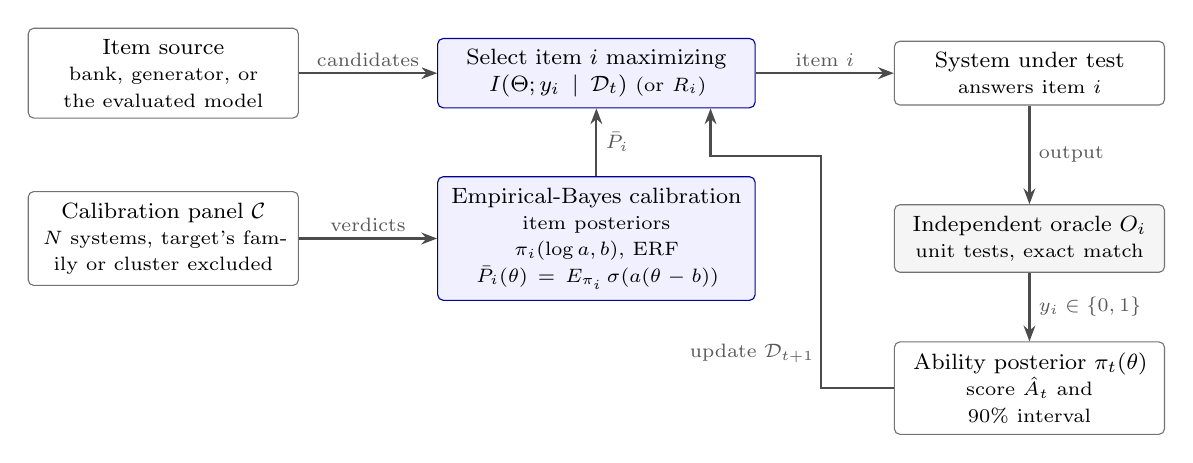
\begin{tikzpicture}[
  font=\footnotesize,
  box/.style={draw=black!55, rounded corners=2pt, align=center, inner sep=4pt, fill=white, text width=3.15cm},
  key/.style={draw=blue!60!black, rounded corners=2pt, align=center, inner sep=4pt, fill=blue!6, text width=3.75cm},
  arr/.style={-{Stealth[length=2mm]}, black!70, thick},
  lab/.style={font=\scriptsize, text=black!65, fill=white, inner sep=1pt}
]
\node[box] (bank) at (0,0) {Item source\\{\scriptsize bank, generator, or the evaluated model}};
\node[key] (sel) at (5.5,0) {Select item $i$ maximizing\\ $I(\Theta;y_i\mid\mathcal D_t)$ {\scriptsize (or $R_i$)}};
\node[box] (sys) at (11.0,0) {System under test\\{\scriptsize answers item $i$}};
\node[box] (panel) at (0,-2.1) {Calibration panel $\mathcal C$\\{\scriptsize $N$ systems, target's family or cluster excluded}};
\node[key] (cal) at (5.5,-2.1) {Empirical-Bayes calibration\\{\scriptsize item posteriors $\pi_i(\log a,b)$, ERF}\\{\scriptsize $\bar P_i(\theta)=\mathbb E_{\pi_i}\,\sigma(a(\theta-b))$}};
\node[box, fill=black!4] (oracle) at (11.0,-2.1) {Independent oracle $O_i$\\{\scriptsize unit tests, exact match}};
\node[box] (post) at (11.0,-4.0) {Ability posterior $\pi_t(\theta)$\\{\scriptsize score $\hat A_t$ and 90\% interval}};
\draw[arr] (bank) -- node[lab, above=1pt]{candidates} (sel);
\draw[arr] (panel) -- node[lab, above=1pt]{verdicts} (cal);
\draw[arr] (cal) -- node[lab, right=2pt]{$\bar P_i$} (sel);
\draw[arr] (sel) -- node[lab, above=1pt]{item $i$} (sys);
\draw[arr] (sys) -- node[lab, right=2pt]{output} (oracle);
\draw[arr] (oracle) -- node[lab, right=2pt]{$y_i\in\{0,1\}$} (post);
\draw[arr] (post.west) -- (8.35,-4.0) -- node[lab, pos=0.15, left=1pt, fill=none]{update $\mathcal D_{t+1}$} (8.35,-1.05) -- (6.95,-1.05) -- (6.95,0 |- sel.south);
\end{tikzpicture}
\caption{EOST-M, the calibration-marginal adaptive test studied in this paper. Item parameters are not plugged in: each item enters the test through its expected response function (ERF) under its empirical-Bayes posterior given a small calibration panel, items are selected one at a time by expected information gain about competence (or by the score-targeted criterion $R_i$ when the estimand is the benchmark score), and verdicts come from an independent oracle. The framework allows items from any source, including the evaluated model, but all evidence in this paper uses fixed banks.}
\label{fig:framework}
\end{figure}

\begin{algorithm}[t]
\caption{EOST-M: calibration-marginal adaptive test with one-step (myopic) expected-information-gain selection}
\label{alg:eost}
\small
\begin{algorithmic}[1]
\Require bank $\mathcal I$ with oracles $O_i$; panel verdicts $Y_{\mathcal C}\in\{0,1\}^{N\times I}$; budget $T$; ability grid $\{\theta_k\}_{k=1}^{K}$
\State $(\hat\theta_{\mathcal C},\cdot)\gets$ joint MAP of the 2PL on $Y_{\mathcal C}$ \Comment{calibrator abilities}
\State $\eta\gets\arg\max_\eta\sum_i\log\sum_g p_\eta(\psi_g)\,p(Y_{\mathcal C,i}\mid\hat\theta_{\mathcal C},\psi_g)$ \Comment{empirical-Bayes item hyperprior (EM)}
\State $W_{ig}\propto p_\eta(\psi_g)\,p(Y_{\mathcal C,i}\mid\hat\theta_{\mathcal C},\psi_g)$ \Comment{item posteriors on the $(\log a,b)$ grid}
\State $\bar P_{ik}\gets\sum_gW_{ig}\,\sigma\big(a_g(\theta_k-b_g)\big)$, \;$H_{ik}\gets h(\bar P_{ik})$ \Comment{expected response functions}
\State $\log\pi_k\gets\log\phi(\theta_k)$;\; $\mathcal U\gets\mathcal I$ (candidate pool)
\For{$t=1,\dots,T$}
  \State $\pi\gets\mathrm{softmax}(\log\pi)$;\; $\bar p_i\gets\sum_k\bar P_{ik}\pi_k$ for $i\in\mathcal U$
  \State $i_t\gets\arg\max_{i\in\mathcal U}\;h(\bar p_i)-\sum_kH_{ik}\pi_k$ \Comment{EIG; or $R_i$ of Eq.~\eqref{eq:evr}}
  \State $y\gets O_{i_t}(\text{system's answer to } i_t)$ \Comment{independent oracle}
  \State $\log\pi_k\gets\log\pi_k+y\log\bar P_{i_tk}+(1-y)\log(1-\bar P_{i_tk})$;\; $\mathcal U\gets\mathcal U\setminus\{i_t\}$
\EndFor
\State $\pi\gets\mathrm{softmax}(\log\pi)$;\; $\bar p_i\gets\sum_k\bar P_{ik}\pi_k$ for all $i$
\State \Return posterior $\pi$, score estimate $\hat A_T=\frac1I\big(\sum_{\text{asked}}y+\sum_{i\notin\text{asked}}\bar p_i\big)$ and its interval
\end{algorithmic}
\end{algorithm}

\section{Theory: what calibration uncertainty does to an adaptive test}
\label{sec:theory}

Throughout, $\pi_t$ denotes the target's ability posterior after $t$ administered
items, $\mu_t$ and $\sigma_t^2$ its mean and variance, $h(p)=-p\log p-(1-p)\log(1-p)$
the binary entropy (nats), and $P_i$ the response function used for item $i$
(plug-in $P_i(\theta)=\sigma(\hat a_i(\theta-\hat b_i))$ or the expected response
function $\bar P_i$ of Eq.~\eqref{eq:erf}). Each result is followed by
its proof.
All optimality statements below are \emph{myopic}: they concern the best next item
given the current posterior, not the best sequential policy over a whole test.

\paragraph{The calibration-marginal model is an exact Bayesian model given the calibrators.}
\begin{lemma}[Exactness given the panel's abilities]\label{lem:exact}
Let the calibrators' abilities $\theta_C$ and the item hyperparameters $\eta$ be fixed.
Then the item parameters $\psi_1,\dots,\psi_I$ are independent a posteriori given the
panel's responses, and for any set $S$ of items answered by a new target with ability
$\theta$,
\begin{equation}\label{eq:factor}
p(y_S\mid\theta,\mathcal D_{\mathrm{panel}},\theta_C,\eta)=\prod_{i\in S}\bar P_i(\theta)^{y_i}\{1-\bar P_i(\theta)\}^{1-y_i},
\qquad \bar P_i(\theta)=\mathbb E\big[P_{\psi_i}(\theta)\mid\mathcal D_{\mathrm{panel}},\theta_C,\eta\big].
\end{equation}
Integrating $\theta_C$ and $\eta$ as well (a fully Bayesian treatment) replaces the
product by
\[
\mathbb E_{\theta_C,\eta\mid\mathcal D}\Big[\prod_{i\in S}\bar P_i^{(\theta_C,\eta)}(\theta)^{y_i}\{1-\bar P_i^{(\theta_C,\eta)}(\theta)\}^{1-y_i}\Big],
\]
which no longer factorizes, because shared abilities and hyperparameters make the items
dependent.
\end{lemma}

\begin{proof}
Given $\theta_C$ and $\eta$, the joint posterior of the item parameters is proportional
to $\prod_i p(\psi_i\mid\eta)\prod_{n}p(y_{ni}\mid\theta_n,\psi_i)$, a product of factors that
each involve one item only; the items are therefore independent a posteriori. The
target's responses are conditionally independent given $(\theta,\psi)$ and each involves
one item, so
$p(y_S\mid\theta,\cdot)=\int\prod_{i\in S}p(y_i\mid\theta,\psi_i)\prod_i p(\psi_i\mid\cdot)\,d\psi
=\prod_{i\in S}\int p(y_i\mid\theta,\psi_i)p(\psi_i\mid\cdot)\,d\psi_i$, and the inner integral
is $\bar P_i(\theta)^{y_i}\{1-\bar P_i(\theta)\}^{1-y_i}$. Integrating over
$(\theta_C,\eta)$ afterwards averages products, not factors, which does not factorize
unless the posterior of $(\theta_C,\eta)$ is a point mass.
\end{proof}

The ability posterior, the predictive distribution and the information criteria of
EOST-M are therefore exact Bayesian quantities \emph{conditional on} point estimates of
the calibrators' abilities and of the hyperprior; nothing is approximated about the item
parameters except the grid. This locates EOST-M precisely with respect to fully Bayesian
adaptive testing \citep{vanderlinden2020fast,fink2025accounting}: those methods also
integrate $\theta_C$ and $\eta$, by Markov chain Monte Carlo. When their sampler draws
stored item parameters independently for each administered item at every iteration, as
the algorithm of \citet{vanderlinden2020fast} does, the ability posterior it targets uses
the per-item averages $\mathbb E_{\theta_C,\eta}[\bar P_i^{(\theta_C,\eta)}]$, i.e.\
Eq.~\eqref{eq:factor} with item marginals that also average over $(\theta_C,\eta)$; we call
this the \emph{posterior-draw marginal} Bayesian CAT, and the version that keeps the product
inside the expectation the \emph{joint fully Bayesian} CAT. The
difference between the two is thus an empirical question about how much the uncertainty
in $(\theta_C,\eta)$ matters; study~2 answers it (Section~\ref{sec:study2}).

\begin{proposition}[Entropy--information decomposition]\label{prop:decomp}
For every item $i$,
\begin{equation}
U_{\mathrm{EIG}}(i)= I(\theta;y_i\mid\mathcal D_t)
= \underbrace{h\big(\bar p_i\big)}_{U_{\mathrm{H}}(i)} \;-\; \mathbb E_{\pi_t}\big[h(P_i(\theta))\big],
\qquad \bar p_i=\mathbb E_{\pi_t}[P_i(\theta)],
\end{equation}
so that $0\le U_{\mathrm{EIG}}(i)\le U_{\mathrm H}(i)$, with equality on the right
if and only if the item is deterministic given $\theta$, $\pi_t$-almost surely.
\end{proposition}

\begin{proof}
$I(\theta;y_i\mid\mathcal D_t)=H(y_i\mid\mathcal D_t)-H(y_i\mid\theta,\mathcal D_t)$.
Given $\mathcal D_t$, $y_i$ is Bernoulli with mean $\bar p_i=\mathbb E_{\pi_t}P_i(\theta)$,
so $H(y_i\mid\mathcal D_t)=h(\bar p_i)$; given $\theta$ it is Bernoulli$(P_i(\theta))$,
so $H(y_i\mid\theta,\mathcal D_t)=\mathbb E_{\pi_t}h(P_i(\theta))\ge0$, with equality iff
$P_i(\theta)\in\{0,1\}$ $\pi_t$-a.s. Non-negativity of mutual information gives
the lower bound. For the plug-in model the item parameters are fixed; for the
marginal model the response of the target to item $i$ given $\theta$ is
Bernoulli$(\bar P_i(\theta))$ because $\psi_i=(\log a_i,b_i)$ appears only in
item $i$'s likelihood and its posterior given the panel does not depend on the
target's other responses, so the same argument applies with $P_i=\bar P_i$.
\end{proof}

Predictive entropy over-values items whose outcome is uncertain \emph{even for a known
competence}: the subtracted term is the item's irreducible noise. EIG is the myopically
optimal choice for information about $\theta$; it is not claimed to be optimal over a
whole test, for which greedy guarantees require additional structure
\citep{golovin2011adaptive}.

\begin{proposition}[Local equivalence with Fisher information]\label{prop:local}
Let $P_i$ be three times continuously differentiable with bounded derivatives
near $\mu_t$, with $P_i(\mu_t)\in(0,1)$, and let $\pi_t$ concentrate,
$\sigma_t\to0$ with $\mathbb E_{\pi_t}|\theta-\mu_t|^3=o(\sigma_t^2)$. Then
\begin{equation}
U_{\mathrm{EIG}}(i)=\tfrac12\,\sigma_t^2\,\mathcal I_i(\mu_t)+o(\sigma_t^2),
\qquad \mathcal I_i(\theta)=\frac{P_i'(\theta)^2}{P_i(\theta)\{1-P_i(\theta)\}},
\end{equation}
while $U_{\mathrm H}(i)=h\big(P_i(\mu_t)\big)+O(\sigma_t^2)$.
\end{proposition}

\begin{proof}
Assume $P_i\in C^3$ with bounded derivatives near $\mu=\mu_t$ and $P_i(\mu)\in(0,1)$.
Write $\delta=\theta-\mu$, $P=P_i(\mu)$, $P'=P_i'(\mu)$, $P''=P_i''(\mu)$. Taylor's
theorem gives $P_i(\theta)=P+P'\delta+\frac12P''\delta^2+O(|\delta|^3)$, hence
$\bar p_i=P+\frac12P''\sigma^2+o(\sigma^2)$ because $\mathbb E\delta=0$,
$\mathbb E\delta^2=\sigma^2$ and $\mathbb E|\delta|^3=o(\sigma^2)$. Since $h$ is smooth on
$(0,1)$, $h(\bar p_i)=h(P)+\frac12h'(P)P''\sigma^2+o(\sigma^2)$ and
$\mathbb E\,h(P_i(\theta))=h(P)+\frac12h'(P)P''\sigma^2+\frac12h''(P)P'^2\sigma^2+o(\sigma^2)$.
(The expansions hold on $|\delta|\le\varepsilon$ for a fixed small $\varepsilon$; since $h$
and $P_i$ are bounded, the contribution of $|\delta|>\varepsilon$ is at most a constant
times $\Pr(|\delta|>\varepsilon)\le\mathbb E|\delta|^3/\varepsilon^3=o(\sigma^2)$.)
Subtracting and using $h''(p)=-1/\{p(1-p)\}$,
$U_{\mathrm{EIG}}(i)=\frac12\sigma^2P'^2/\{P(1-P)\}+o(\sigma^2)=\frac12\sigma^2\mathcal I_i(\mu)+o(\sigma^2)$.
The statement for $U_{\mathrm H}$ is the first expansion.
\end{proof}

\begin{corollary}[Entropy is blind to discrimination]\label{cor:blind}
Under the 2PL model,
\[
\mathcal I_i(\mu)=a_i^2P_i(\mu)\{1-P_i(\mu)\}.
\]
Two items
with the same success probability $P_i(\mu_t)=p$ are tied by predictive entropy
while their information ratio is $(a_1/a_2)^2$, so the two criteria rank them
differently whenever $a_1\neq a_2$. When all items share one discrimination, both
$h(P_i(\mu_t))$ and $\mathcal I_i(\mu_t)$ are strictly decreasing in
$|P_i(\mu_t)-\tfrac12|$, hence entropy sampling, maximum Fisher information and EIG
induce the same ranking to leading order: under a common discrimination, entropy
sampling is optimal by accident.
\end{corollary}

\begin{proof}
For the 2PL, $P_i'=a_iP_i(1-P_i)$, so $\mathcal I_i=a_i^2P_i(1-P_i)$. With a common
$a$, $\mathcal I_i$ and $h(P_i)$ are both strictly decreasing functions of
$|P_i-\frac12|$, hence order-equivalent.
\end{proof}

The corollary gives a sufficient condition for agreement (a common discrimination) and
a constructive source of disagreement (ties in $p$ with unequal $a$); it does not claim
that equal discriminations are necessary for two rankings to coincide on a particular
bank. Proposition~\ref{prop:local} also implies that EIG, posterior-weighted Fisher
information and maximum Fisher information agree to first order; differences between
them are early-test phenomena \citep{chen2000comparison}. The decisive difference comes
from calibration uncertainty.

\begin{proposition}[Information cap under calibration uncertainty]\label{prop:cap}
Let $G$ be a continuous distribution function (logistic for the 2PL, $\Phi$ for the
normal ogive), let the item response function be $P_\psi(\theta)=G\big(a(\theta-b)\big)$,
and let the difficulty given the panel be $b\mid a\sim\mathcal N(\bar b,s^2)$. Then the
Fisher information about $\theta$ carried by a response under the expected response
function satisfies, for every $\theta$ and every $a$,
\begin{equation}\label{eq:cap}
\bar{\mathcal I}(\theta)=\frac{\bar P'(\theta)^2}{\bar P(\theta)\{1-\bar P(\theta)\}}\le\frac{2}{\pi s^2},
\end{equation}
and the bound is attained in the limit $a\to\infty$. For the normal ogive the expected
response function is exactly $\Phi\big(a^{\mathrm{eff}}(\theta-\bar b)\big)$ with
$a^{\mathrm{eff}}=a/\sqrt{1+a^2s^2}<1/s$.
\end{proposition}

\begin{proof}
Fix $a>0$ and let $L$ have distribution function $G$, independent of
$b\sim\mathcal N(\bar b,s^2)$ (conditionally on $a$). Since
$G(a(\theta-b))=\Pr(L/a+b\le\theta\mid b)$, the expected response function is
$\bar P(\theta)=\Pr(L/a+b\le\theta)$, so a response can be represented as
$y=\mathbf 1\{L/a+b\le\theta\}$. Consider the augmented observation $(y,L)$. The
distribution of $L$ does not depend on $\theta$, so its Fisher information is
$\mathcal I_{(y,L)}(\theta)=\mathbb E_L\big[\mathcal I_{y\mid L}(\theta)\big]$. Given $L=\ell$,
$y$ is Bernoulli with success probability
$\Pr(b\le\theta-\ell/a)=\Phi(u)$, $u=(\theta-\ell/a-\bar b)/s$, whose information is
$s^{-2}\phi(u)^2/\{\Phi(u)(1-\Phi(u))\}\le s^{-2}\cdot\frac2\pi$, the maximum being
attained at $u=0$ where $\phi(0)^2=(2\pi)^{-1}$ and $\Phi(0)(1-\Phi(0))=\frac14$. Hence
$\mathcal I_{(y,L)}(\theta)\le2/(\pi s^2)$. (For a difficulty posterior with any distribution
function $F$ and density $f$, the success probability given $L=\ell$ is $F(\theta-\ell/a)$, with
information $f^2/\{F(1-F)\}$ at that point, which gives the general bound stated after this
proof.) The response $y$ is a statistic of $(y,L)$, and
the Fisher information of a statistic never exceeds that of the data it is computed from:
the score of $y$ is the conditional expectation of the score of $(y,L)$ given $y$, whose
variance is at most the variance of the latter \citep{zamir1998proof}. Therefore
$\bar{\mathcal I}(\theta)=\mathcal I_y(\theta)\le\mathcal I_{(y,L)}(\theta)\le2/(\pi s^2)$.
If $a$ is itself uncertain, the same argument conditions on $(a,L)$. As $a\to\infty$,
$L/a\to0$ and $\bar P(\theta)\to\Phi((\theta-\bar b)/s)$, whose information at
$\theta=\bar b$ is $2/(\pi s^2)$, so the bound is sharp. For the normal ogive,
$L\sim\mathcal N(0,1)$ and $L/a+b\sim\mathcal N(\bar b,a^{-2}+s^2)$, which gives
$\bar P(\theta)=\Phi\big(a^{\mathrm{eff}}(\theta-\bar b)\big)$ with
$a^{\mathrm{eff}}=a/\sqrt{1+a^2s^2}$ and maximal information $\frac2\pi(a^{\mathrm{eff}})^2<2/(\pi s^2)$.
\end{proof}

The bound holds exactly for the logistic 2PL used in this paper; no probit approximation
is involved. In words, the proof represents a response as $y=\mathbf 1\{L/a+b\le\theta\}$ with $L$
distributed as $G$ independently of $b$: given $L$, the response is a probit item with
discrimination $1/s$, whose information never exceeds $2/(\pi s^2)$, and discarding $L$
cannot increase Fisher information \citep{zamir1998proof}. A unit test checks the bound
numerically for the logistic link over a grid of $(a,s,\theta)$. The Gaussian form of the
difficulty posterior enters only through the conditional item given $L$: the same argument gives
$\bar{\mathcal I}(\theta)\le\sup_u f(u)^2/\{F(u)(1-F(u))\}$ for any difficulty posterior with
distribution function $F$ and density $f$ (for a logistic posterior with standard deviation
$s$ this is $\pi^2/(12s^2)\approx0.82/s^2$, against $2/(\pi s^2)\approx0.64/s^2$ for a Gaussian
one), whereas a posterior concentrated on a few points gives no useful bound. Our grid
posteriors are discrete approximations of smooth posteriors, so for them the Gaussian cap
indicates the order of magnitude rather than a guarantee.

\begin{corollary}[Averaging information is not integrating uncertainty]\label{cor:jensen}
For any item-parameter posterior, the information of the expected response
function never exceeds the posterior-expected Fisher information,
$\bar{\mathcal I}_i(\theta)\le\mathbb E_{\pi_i}\big[\mathcal I_{i,\psi}(\theta)\big]$.
\end{corollary}

\begin{proof}
For a binary response, $\mathcal I=P'^2/\{P(1-P)\}=P'^2/P+P'^2/(1-P)$. The
map $(x,y)\mapsto x^2/y$ is jointly convex on $\mathbb R\times(0,\infty)$, so
$\mathcal I$ is a jointly convex function of $(P,P')$. The expected response
function and its derivative are the posterior averages
$(\bar P_i,\bar P_i')=\mathbb E_{\pi_i}[(P_{i,\psi},P_{i,\psi}')]$, and Jensen's inequality
gives $\bar{\mathcal I}_i(\theta)\le\mathbb E_{\pi_i}[\mathcal I_{i,\psi}(\theta)]$.
\end{proof}

Criteria that average Fisher information over parameter uncertainty---the Bayesian
maximum-information criterion of fully Bayesian adaptive testing
\citep{vanderlinden2020fast,fink2025accounting} and Laplace-approximated variants
\citep{mandujano2026laplace}---can therefore be optimistic about poorly calibrated items
and do not inherit the cap of Proposition~\ref{prop:cap}. (Empirically this optimism did
not change which items were worth asking; Sections~\ref{sec:strong} and~\ref{sec:study2}.)
Under the plug-in model the information of an item is $\hat a_i^2/4$ at its
difficulty, unbounded in the point estimate $\hat a_i$. Items whose responses
are perfectly separated in a small panel (solved by every strong calibrator and
by no weak one, or by none) are exactly those with inflated $\hat a_i$ and large
$s_i$; plug-in selection therefore concentrates on them, the classical
\emph{capitalization on calibration error} \citep{vanderlinden2000capitalization,patton2013influence}.
The expected response function removes the incentive automatically: its information is
capped---by $2/(\pi s_i^2)$ for a Gaussian difficulty posterior, by the general bound above
otherwise---whatever $\hat a_i$ is. A shrinkage prior on $a_i$ limits the
inflation of $\hat a_i$, but not the uncertainty $s_i$ about where the item sits.

\paragraph{Myopic score-targeted design.}
Practitioners often care about the full-bank accuracy $A=\frac1I\sum_iy_i$
rather than about $\theta$. Let $U$ be the set of unobserved items and
$S_U=\sum_{k\in U}y_k$. The score-targeted criterion (EVR) asks the item that
minimizes the expected posterior variance of $S_U$ after one more response.

\begin{proposition}[One-step score-targeted design]\label{prop:evr}
For $i\in U$ let
\[
v_i=\bar p_i(1-\bar p_i),\qquad M_{-i}(\theta)=\sum_{k\in U\setminus\{i\}}P_k(\theta),\qquad
c_i=\mathrm{Cov}_{\pi_t}\big(P_i(\theta),M_{-i}(\theta)\big).
\]
The expected one-step variance reduction obtained by asking $i$ is exactly
\begin{equation}\label{eq:evr}
R_i=\mathrm{Var}(S_U\mid\mathcal D_t)-\mathbb E_{y_i}\big[\mathrm{Var}(S_{U\setminus\{i\}}\mid\mathcal D_t,y_i)\big]
=\frac{(v_i+c_i)^2}{v_i}.
\end{equation}
Under the conditions of Proposition~\ref{prop:local}, and if
$P_i'(\mu_t)M_{-i}'(\mu_t)\neq0$, then
\[
c_i=\sigma_t^2P_i'(\mu_t)M_{-i}'(\mu_t)\{1+o(1)\},\qquad
R_i=v_i+2c_i+\sigma_t^4M_{-i}'(\mu_t)^2\,\mathcal I_i(\mu_t)\{1+o(1)\}.
\]
\end{proposition}

\begin{proof}
Write $S_U=y_i+S_{-i}$. By the law of total variance,
$\mathbb E_{y_i}[\mathrm{Var}(S_{-i}\mid y_i)]=\mathrm{Var}(S_{-i})-\mathrm{Var}(\mathbb E[S_{-i}\mid y_i])$, so
$R_i=\mathrm{Var}(y_i)+2\,\mathrm{Cov}(y_i,S_{-i})+\mathrm{Var}(\mathbb E[S_{-i}\mid y_i])$ (all moments
conditional on $\mathcal D_t$). Here $\mathrm{Var}(y_i)=v_i$. Responses are conditionally
independent given $\theta$, so $\mathrm{Cov}(y_i,S_{-i})=\mathrm{Cov}_{\pi_t}(P_i(\theta),M_{-i}(\theta))=c_i$.
Because $y_i$ is binary, $\mathbb E[S_{-i}\mid y_i]$ is affine in $y_i$ with slope
$c_i/v_i$, so $\mathrm{Var}(\mathbb E[S_{-i}\mid y_i])=c_i^2/v_i$ and $R_i=(v_i+c_i)^2/v_i$.
Under the assumptions of Proposition~\ref{prop:local}, write
$P_i(\theta)=P+P'\delta+r_1(\delta)$ and $M_{-i}(\theta)=M+M'\delta+r_2(\delta)$ with
$|r_k(\delta)|\le C\delta^2$ (derivatives at $\mu$, as in the proof of Proposition~\ref{prop:local}). Since $\mathbb E\delta=0$,
$c_i=P'M'\sigma^2+P'\,\mathbb E[\delta r_2]+M'\,\mathbb E[\delta r_1]+\mathrm{Cov}(r_1,r_2)$; the
last three terms are $O(\mathbb E|\delta|^3+\mathbb E\delta^4)=o(\sigma^2)$ because the ability
grid is bounded, so that $\mathbb E\delta^4\le C'\,\mathbb E|\delta|^3$. Hence
$c_i=\sigma^2P'M'\{1+o(1)\}$ when $P'M'\neq0$, and with $v_i=P(1-P)\{1+O(\sigma^2)\}$,
$c_i^2/v_i=\sigma^4M'^2P'^2/\{P(1-P)\}\{1+o(1)\}=\sigma^4M'^2\mathcal I_i(\mu)\{1+o(1)\}$.
\end{proof}

The first term of $R_i$ is a monotone transform of predictive entropy (own outcome
uncertainty); the last is Fisher information weighted by the squared sensitivity of the
remaining bank to $\theta$. One-step score-targeted selection therefore behaves like
uncertainty sampling once competence is pinned down ($\sigma_t^2M'\to0$) and like
information sampling while it is not; because $M'$ grows with the number of unobserved
items, the information regime lasts longer on larger banks (Section~\ref{sec:curves}
finds this tendency). ``Information-optimal'' is thus relative to an estimand and to a
one-step horizon: EIG maximizes the next response's information about competence, and
$R_i$ the next response's reduction of score variance.

\section{Experimental design}
\label{sec:design}

\subsection{Data}
\begin{table}[tbp]
\centering\scriptsize
\caption{Real response matrices. Verdict: one deterministic evaluation per system and item (single) or a recorded pass rate over several samples binarized at one half (aggregate; TruthfulQA: continuous MC2 score binarized). $J$ systems, $F$ heuristic families, $I$ items; accuracy range across systems; items solved by no system. Role: confirmatory in studies 1 and 2, or development bank used only to design the protocols (Sections~\ref{sec:dev} and~\ref{sec:design2}). SE: software engineering.}
\label{tab:data}
\setlength{\tabcolsep}{2.6pt}
\begin{tabular}{@{}lllllrrrcr@{}}
\toprule
Bank & Role & Domain & Oracle & Verdict & $J$ & $F$ & $I$ & Accuracy & Unsolved \\
\midrule
GSM8K & 1, 2 & math & numeric match & single & 395 & 227 & 1319 & 0.00--0.77 & 13 \\
ARC-C & 1, 2 & multiple choice & log-lik.\ choice & single & 395 & 227 & 1172 & 0.26--0.73 & 51 \\
HellaSwag & 1, 2 & multiple choice & log-lik.\ choice & single & 395 & 227 & 2000 & 0.31--0.90 & 43 \\
WinoGrande & 1, 2 & multiple choice & log-lik.\ choice & single & 395 & 227 & 1267 & 0.59--0.87 & 1 \\
MMLU & 1, 2 & multiple choice & log-lik.\ choice & single & 395 & 227 & 2000 & 0.26--0.80 & 0 \\
SWE-bench V. & 1, 2 & agentic SE & repository tests & single & 175 & 123 & 500 & 0.00--0.79 & 26 \\
LiveCodeBench & 1, 2 & code generation & hidden tests & aggregate & 28 & 15 & 1055 & 0.23--0.87 & 46 \\
CRUXEval-O & 1, 2 & code reasoning & execution & aggregate & 31 & 12 & 800 & 0.22--0.78 & 98 \\
SWE-bench Lite & dev. & agentic SE & repository tests & single & 84 & 49 & 300 & 0.00--0.60 & 35 \\
CRUXEval-I & dev. & code reasoning & execution & aggregate & 31 & 12 & 800 & 0.14--0.78 & 59 \\
TruthfulQA & dev. & multiple choice & log-lik.\ choice & aggregate & 395 & 227 & 817 & 0.30--0.73 & 47 \\
\bottomrule
\end{tabular}
\end{table}

We use public item-level verdicts of real systems (Table~\ref{tab:data}). Open LLM
Leaderboard \citep{beeching2023openllm} verdicts for 395 models on GSM8K
\citep{cobbe2021gsm8k}, ARC-Challenge \citep{clark2018arc}, HellaSwag
\citep{zellers2019hellaswag}, WinoGrande \citep{sakaguchi2020winogrande}, MMLU
\citep{hendrycks2021mmlu} and TruthfulQA \citep{lin2022truthfulqa} are taken from the
release of \citet{polo2024tinybenchmarks}; HellaSwag and MMLU are uniformly subsampled to
2,000 items with a fixed seed, and TruthfulQA's continuous MC2 score is binarized at 0.5.
SWE-bench Verified and Lite \citep{jimenez2024swebench} verdicts (instance resolved by the
official harness) come from the public submissions repository (175 and 84 systems).
LiveCodeBench \citep{jain2025livecodebench} pass rates for 28 models on 1,055 problems and
CRUXEval \citep{gu2024cruxeval} pass rates of temperature-0.2 samples for 31 models are
binarized at one half; these two banks therefore carry recorded aggregate verdicts
(Section~\ref{sec:framework}), the other six deterministic ones. Every source is pinned to
a git commit and every processed matrix carries a SHA-256 hash.

\paragraph{Synthetic banks.} Three simulated banks with known abilities complement the
real data (300 systems, 600 items each, $\theta\sim\mathcal N(0,1)$,
$\log a\sim\mathcal N(0,0.5^2)$, $b\sim\mathcal N(0,1.5^2)$): a well-specified 2PL bank; a
bank in which 60\% of the items have a guessing floor of 0.25; and a bank in which half of
the items depend on a second ability dimension correlated 0.6 with the first. The fitted
model is always the unidimensional 2PL. Synthetic results never enter a confirmatory
decision.

\paragraph{Families and strict clusters.} Systems that share an underlying model are
not independent. \emph{Heuristic families} are defined by organization namespace (Open
LLM Leaderboard), by model line including reasoning-effort and version variants
(LiveCodeBench, CRUXEval), and, for SWE-bench, by the set of underlying LLMs declared in a
submission's metadata (two agentic systems are related if they share any LLM). Heuristic
families miss renamed copies, merges and fine-tunes across organizations, so study~2 uses
\emph{strict clusters}: connected components of the graph that joins two systems if they
share a heuristic family or if the correlation of their standardized 2PL residuals is at
least 0.5---they share at least half of their idiosyncratic error pattern beyond what
ability explains. Residuals are pooled over banks that share systems (the six Open LLM
Leaderboard banks; CRUXEval-O and -I). Agreement measures such as Cohen's $\kappa$ were
not usable for this purpose: on HellaSwag, $\kappa\ge0.8$ chains 353 of 395 systems into
one component because all strong models agree on most items. The strict clusters number
\ClusOLLB\ on the Open LLM Leaderboard (largest \ClusOLLBMax\ systems), \ClusSWE\ on
SWE-bench Verified, \ClusLCB\ on LiveCodeBench and \ClusCRUX\ on CRUXEval.

\subsection{Study 1: frozen plan, leave-family-out replay}\label{sec:dev}
For each bank, up to 60 targets were drawn stratified by accuracy decile (all systems
for LiveCodeBench and CRUXEval). For each target and replicate $r=1,\dots,5$, a holdout of
20\% of the items was drawn and shared by all policies and panel sizes; for each panel
size $N\in\{4,8,16,32,64\}$ a panel was drawn outside the target's heuristic family. The
twelve policies of Section~\ref{sec:framework} (five criteria under both models, PWFI
under the marginal model only, plus Naive) were replayed on the target's recorded
verdicts with a budget of $T=100$ items. All random streams derive from one master seed
by hashing (bank, purpose, target, replicate, $N$, policy).

The protocol was designed on development banks only (SWE-bench Lite, CRUXEval-I,
TruthfulQA, synthetic 2PL; Section~\ref{sec:devhist}), where one problem appeared: with
fixed weakly-informative priors, items solved by no calibrator were shrunk towards an
arbitrary difficulty, so empirical-Bayes hyperpriors were adopted for every policy. The
plan (banks, protocol, endpoints, four hypotheses, tests, multiplicity control, decision
rule), the analysis code and the data manifests were then hashed and committed before any
confirmatory run, and the run wrapper refuses to start if a frozen file changes. No public
registry or external time stamp was used, so we call this a \emph{frozen analysis plan}
rather than a preregistration \citep{nosek2018preregistration}; the git history shows the
freeze commit before every confirmatory artifact.

\paragraph{Hypotheses} (primary panel size $N=8$):
\textbf{H1} EIG:mg has lower integrated holdout log loss than Entropy:mg;
\textbf{H2} EIG:mg has lower integrated holdout log loss than MFI:pi;
\textbf{H3} EIG:mg has lower integrated score error than Naive subsampling;
\textbf{H4} EIG:mg's 90\% score intervals are better calibrated than MFI:pi's
($|\mathrm{coverage}-0.9|$). Each contrast is a two-sided Wilcoxon signed-rank test
\citep{wilcoxon1945individual} on paired per-target values (replicates averaged within
target), with Holm correction \citep{holm1979simple} over the whole family
(8 banks $\times$ panel sizes $\times$ 4 hypotheses); a hypothesis is \emph{supported} if,
at $N=8$, the adjusted test favours EOST-M in at least five of the eight banks and the
baseline in none. Because targets of one family are not independent, every study-1
contrast is also re-analysed post hoc with heuristic families and with strict clusters as
units (cluster means, the same tests and decision rule).

\subsection{Study 2: independent targets and strong competitors}\label{sec:design2}
Study~2 was designed after an external review of study~1 and frozen before execution
(plan, hypotheses, cluster file and code hashed and committed; the plan and its hash were
also sent to the first author, outside the execution environment, before the first run).
It differs from
study~1 in four ways. \emph{Targets} are one randomly chosen representative per strict
cluster (systems that were not study-1 targets preferred), at most 40 per bank, stratified
by accuracy, so targets are independent units; \emph{panels} ($N\in\{4,8,16\}$, three
replicates, new seeds) exclude the target's whole strict cluster. \emph{Competitors} are
the strongest we could identify:
\begin{itemize}\itemsep0pt
\item \textsc{MFI:1pr}, a regularized Rasch-type plug-in CAT (one common discrimination
with $\log a\sim\mathcal N(0,0.05^2)$, empirical-Bayes prior on $b$), and
\textsc{EIG:1prmg}, the same model integrated (both found post hoc in study~1);
\item \textsc{FB:bmi} and \textsc{FB:eig}, a \emph{posterior-draw marginal Bayesian CAT} (PDM
Bayesian CAT; called the fully Bayesian CAT in the frozen plan): a Gibbs sampler for the
hierarchical 2PL of the panel (abilities, item parameters on the grid, hyperparameters,
with a translation move for the overall location), eight retained draws, and the
target's posterior computed with each item's response function averaged over the draws
separately (the target of \citealp{vanderlinden2020fast}; Lemma~\ref{lem:exact} shows that
this integrates the calibrators' abilities and the hyperprior item by item, not jointly);
selection by Bayesian maximum information
(posterior-weighted expected Fisher information, the strategy recommended by
\citealp{fink2025accounting}) or by EIG ($N\in\{4,8\}$);
\item \textsc{Random:mg}, random items scored with the EOST-M model, which isolates the
value of adaptivity from that of the calibration;
\item \textsc{ATLAS}, an ATLAS-style CAT \citep{li2026atlas}: 3PL with the lower asymptote
fixed at the chance rate of the item format (ARC-C, HellaSwag, MMLU $0.25$, WinoGrande
$0.5$, others 0), first item closest in difficulty to 0, then a uniform draw among the five
most informative items at the expected a posteriori (EAP) ability \citep{kingsbury1989procedures};
\item \textsc{tinyBenchmarks} \citep{polo2024tinybenchmarks}: anchor items by K-Means on
the panel's item embeddings and the gp-IRT estimator, at budgets of 25, 50 and 100 items;
\textsc{MINCE} \citep{das2026mince}: Monte Carlo sizing on the panel and the plain mean of
one frozen random subset, at the same budgets and at its own size $n^\star$;
\item \textsc{MFI:pi} and \textsc{Naive} as in study~1, two empirical-Bayes variants of
EOST-M (cross-fitted hyperprior; Student-$t$ hyperprior family) and an exploratory mixed
policy (every fourth item uniform at random).
\end{itemize}
\emph{Intervals} of EOST-M and of the Rasch-type test are also reported after the
leave-one-calibrator-out recalibration of Section~\ref{sec:framework}. \emph{Hypotheses}
(all at $N=8$, Holm over 11 superiority hypotheses $\times$ 8 banks; supported with
$\ge5$ banks for EOST-M and none against): replications of H2--H4 with independent targets
(R2--R4); EOST-M versus the Rasch-type plug-in (C1) and marginal (C2) tests on log loss;
versus Random:mg on score error (C4); recalibrated versus raw EOST-M intervals (C5b) and
versus Naive's Wilson intervals (C6) on the interval score; versus ATLAS-style CAT on score
error (C7); versus tinyBenchmarks (C8) and MINCE (C9) on the absolute score error after 50
items. In addition, the PDM Bayesian CAT and EOST-M are declared practically equivalent
(C3) if the 90\% bootstrap interval of their relative log-loss difference lies within
$\pm1\%$ on at least six banks, and the recalibrated EOST-M interval is declared calibrated
(C5a) if its mean coverage lies in $[0.85,0.95]$ on at least six banks. A \emph{temporal
component} on SWE-bench Verified uses the latest quarter of submissions by date as targets
and only earlier submissions as calibrators ($N=8$); the synthetic banks are a secondary
component. During the run, before any result was inspected, an independent review of the
code found two problems---tinyBenchmarks can use fewer anchors than its budget, and the
burn-in of the Bayesian sampler was too short on some banks---whose post hoc
corrections were specified in the research log before the results were looked at; the
frozen run was completed unchanged and every frozen decision is reported as computed
(Section~\ref{sec:deviations}, deviation xiii).

\paragraph{Implementation of the competitors.} The \emph{Bayesian CATs} run a Gibbs sampler on the
panel's hierarchical 2PL: (1) every item's grid point is drawn from its exact conditional
grid posterior; (2) every calibrator's ability is drawn by griddy Gibbs on 65 points
spanning $\pm0.8$ around its current value; (2b) all abilities and difficulties and the
difficulty mean are shifted by a common multiple of the difficulty grid step (at most 16
steps either way) drawn from its conditional, which only involves the ability prior (the
likelihood and the difficulty hyperprior are invariant); shifts that would move any
sampled difficulty off the grid are excluded, so the move is exact only within these
bounds and rarely acts when many difficulties sit near the edge of the grid; (3) the
hyperparameters are drawn from their conjugate conditionals (flat means, Jeffreys standard
deviations). The chain starts at EOST-M's estimates; in the frozen plan, 8 draws are kept
every 4 sweeps after a burn-in of 10 sweeps, and each contributes its exact conditional item
posterior (Rao--Blackwellization). As noted above, this burn-in proved too short on some banks; the
post hoc correction (60 sweeps) is described in Section~\ref{sec:s2fb}. In 300-sweep chains on the
development banks (\texttt{scripts/fb\_mixing.py}), the translation move removed the slow
mixing of the overall location: the lag-3 autocorrelation of the mean calibrator ability
fell from \MixLocWithoutMin--\MixLocWithoutMax\ without the move to at most \MixLocWithMax\
with it. That location is genuinely uncertain---its posterior standard deviation was
\MixLocSdFour, \MixLocSdEight\ and \MixLocSdSixteen\ for $N=4$, 8 and 16, close to
$1/\sqrt N$ as implied by the $\mathcal N(0,1)$ ability prior---but it shifts abilities and
difficulties together. Scale hyperparameters mix more slowly (lag-3 autocorrelation of
$\sigma_a$ between \MixScaleMin\ and \MixScaleMax), so the eight retained draws represent
their uncertainty only roughly. Follow-up RF2 (Section~\ref{sec:rf2}) measured this with
four long chains, and exploratory follow-ups added the missing moves.

The \emph{ATLAS-style} test fits a 3PL with fixed lower asymptote by grid MAP given the
panel's abilities and the empirical-Bayes prior. \emph{tinyBenchmarks} uses K-Means (best of
five k-means++ restarts) on $(a_i,a_ib_i)$ of the panel's plug-in 2PL fit, the item nearest
to each centroid as anchor, cluster fractions as weights, the bounded maximum-likelihood
ability for p-IRT, and $\lambda=\hat b^2/(\hat v/(4n)+\hat b^2)$ with $\hat b$ the
leave-one-calibrator-out error of the IRT prediction and $\hat v$ the mean Bernoulli
variance of the calibrators. \emph{MINCE} draws 2,000 random subsets per candidate size
(steps of 25) and stops when the 95th percentile of the worst-case drift over calibrators
improves by less than one point.

\subsection{From the pilot program to the frozen plans}\label{sec:devhist}\label{sec:pilot}

\paragraph{Pilot program (historical).} Before study~1, the framework (EOST in our project) was developed through a staged pilot
program on math word problems with \texttt{Qwen3-8B} as target, greedy decoding
and exact numeric oracles, including self-generated items with an independent oracle
(the self-testing aspect of the framework). Every stage had an explicit pass/fail gate
fixed in advance. We report the stages \emph{as recorded in the frozen project log},
including failed gates and the subsequent corrections, because they motivated
the design of Sections~\ref{sec:framework}--\ref{sec:design}. Stages S0--S4 were
executed before the project's Docker-only rule; the S4B run of one model was executed in
the project's earlier container runtime, which differs from the runtime of this paper
(Section~\ref{sec:repro}). Their raw artifacts are archived with SHA-256 hashes but they
were \emph{not} re-executed for this paper, and none of the paper's claims rests on them.
Table~\ref{tab:pilot} summarizes them.

\begin{table}[htbp]
\centering\footnotesize
\caption{Pilot program (historical values from the frozen project log; not re-executed here).
AUIC: area under the information curve; IG: expected-information-gain policy (EOST).}
\label{tab:pilot}
\setlength{\tabcolsep}{4pt}
\begin{tabular}{@{}p{0.9cm}p{4.2cm}p{9.4cm}@{}}
\toprule
Stage & Setting & Recorded outcome and gate \\
\midrule
S0 & Synthetic latent-trait simulator, 30 seeds; IG vs.\ entropy, random, difficulty-matched &
IG $>$ entropy on entropy reduction (6.77 vs.\ 6.51; Holm $p=2.8\times10^{-9}$) and AUIC (5.29 vs.\ 5.12; rank-biserial 1.0). \textbf{Pass}. \\
S1-R2 & GSM-Symbolic, 45 items; 4 calibration conditions (two Qwen3 checkpoints $\times$ thinking on/off) &
Conditions were not independent systems. \textbf{Gate fail}. \\
S1-R3 & Same bank, regularized 2PL & IG AUIC 0.950 vs.\ entropy 0.923 (29/30 seeds); identical final holdout. Exploratory. \\
S2 & LLM-generated items, procedural oracle (75 items, 5 families) &
After fixing a numeric-tolerance bug: IG AUIC 1.224 vs.\ 1.139 (27/30 seeds, $p=1.2\times10^{-4}$); gains early in the test, endpoint saturated, log-loss tail risk. Publication gate \textbf{fail}. \\
S3 & Circularity: self-, external- and procedurally-generated items (45 matched triplets) &
Self minus external accuracy 0.089 (95\% CI $[0,0.2]$, McNemar $p=0.22$): no \emph{detectable} circularity gap at this power (not equivalence). \\
S4 & GSM8K, GSM-Hard, SVAMP, ASDiv (240 items); 4 calibration conditions &
Macro AUIC IG 0.967 vs.\ entropy 0.858 (30/30 seeds). Original gate \textbf{fail} (predictive non-inferiority). An audit found the original Brier holdout was policy-dependent; with a common fixed holdout, integrated Brier 0.0936 vs.\ 0.0969 (24/30 seeds, $p=3.1\times10^{-5}$), final Brier tie (16/30). GSM-Hard went the other way (Brier 0.195 vs.\ 0.183). 2PL weakly identified: 7 distinct $b$, 50.8\% of $a$ at the upper bound. \\
S4B & Expanding the calibration panel to independent systems &
Six calibrators passed a post-hoc parser audit (parse failures within the project's internal 5\% threshold); a seventh, community checkpoint produced 235/240 truncated generations---a generation-protocol failure, not a capability measurement---and is classified as invalid for calibration. Incomplete; not analysed. \\
\bottomrule
\end{tabular}
\end{table}

Three lessons from the pilot shaped EOST v2. First, the information advantage
of IG over predictive entropy was consistent across synthetic, self-generated
and multi-benchmark settings, but it was concentrated early in the test, as
Proposition~\ref{prop:local} predicts. Second, predictive evaluation must use a
holdout shared by all policies; the policy-dependent holdout of the original S4
analysis produced a spurious non-inferiority failure, which we keep reported as
such. Third, and most important, a calibration panel of four conditions drawn
from two checkpoints cannot identify a 2PL: half of the discriminations
saturated at the optimizer bound, the textbook setting for capitalization on
chance (Proposition~\ref{prop:cap}). The confirmatory study therefore targets
exactly this small-panel regime, with independent systems, leave-family-out
panels and calibration-marginal selection.

\paragraph{Development runs.} The development runs on the development banks that shaped both
protocols are summarized in Table~\ref{tab:dev}; the switch to empirical-Bayes hyperpriors
described in Section~\ref{sec:dev} was decided there, before the plan of study~1 was frozen.

\begin{table}[tbp]
\centering\scriptsize
\caption{Development phase (exploratory; 30 targets, 3 replicates). The switch from fixed to empirical-Bayes (EB) item hyperpriors was decided here, before freezing the confirmatory plan.}
\label{tab:dev}
\begin{tabular}{@{}llrrrrrrr@{}}
\toprule
 & & & \multicolumn{2}{c}{holdout log loss} & \multicolumn{2}{c}{score IAE} & \multicolumn{2}{c}{coverage} \\
\cmidrule(lr){4-5}\cmidrule(lr){6-7}\cmidrule(lr){8-9}
Bank & prior & $N$ & EIG:mg & MFI:pi & EIG:mg & MFI:pi & EIG:mg & MFI:pi \\
\midrule
Synth. 2PL & fixed & 4 & 0.5762 & 0.6410 & 0.0433 & 0.0543 & 0.78 & 0.55 \\
SWE-bench Lite & fixed & 4 & 0.4133 & 0.4110 & 0.0430 & 0.0406 & 0.74 & 0.69 \\
CRUXEval-I & fixed & 4 & 0.4833 & 0.5054 & 0.0342 & 0.0441 & 0.88 & 0.63 \\
TruthfulQA & fixed & 4 & 0.4215 & 0.4179 & 0.0335 & 0.0395 & 0.87 & 0.66 \\
Synth. 2PL & fixed & 8 & 0.5371 & 0.5696 & 0.0382 & 0.0427 & 0.77 & 0.59 \\
SWE-bench Lite & fixed & 8 & 0.3743 & 0.3773 & 0.0349 & 0.0292 & 0.74 & 0.75 \\
CRUXEval-I & fixed & 8 & 0.4460 & 0.4659 & 0.0315 & 0.0400 & 0.80 & 0.55 \\
TruthfulQA & fixed & 8 & 0.3726 & 0.3755 & 0.0264 & 0.0305 & 0.83 & 0.64 \\
Synth. 2PL & fixed & 64 & 0.4914 & 0.4931 & 0.0290 & 0.0275 & 0.77 & 0.80 \\
SWE-bench Lite & fixed & 64 & 0.3254 & 0.3267 & 0.0264 & 0.0250 & 0.80 & 0.81 \\
TruthfulQA & fixed & 64 & 0.3204 & 0.3214 & 0.0223 & 0.0237 & 0.70 & 0.64 \\
Synth. 2PL & EB & 4 & 0.5711 & 0.5884 & 0.0424 & 0.0475 & 0.87 & 0.78 \\
SWE-bench Lite & EB & 4 & 0.4036 & 0.4207 & 0.0393 & 0.0371 & 0.77 & 0.69 \\
CRUXEval-I & EB & 4 & 0.4833 & 0.5113 & 0.0365 & 0.0452 & 0.83 & 0.64 \\
TruthfulQA & EB & 4 & 0.4110 & 0.4323 & 0.0367 & 0.0392 & 0.77 & 0.64 \\
Synth. 2PL & EB & 8 & 0.5332 & 0.5403 & 0.0359 & 0.0407 & 0.92 & 0.82 \\
SWE-bench Lite & EB & 8 & 0.3649 & 0.3730 & 0.0296 & 0.0293 & 0.83 & 0.79 \\
CRUXEval-I & EB & 8 & 0.4450 & 0.4702 & 0.0326 & 0.0416 & 0.79 & 0.53 \\
TruthfulQA & EB & 8 & 0.3679 & 0.3851 & 0.0284 & 0.0308 & 0.78 & 0.65 \\
Synth. 2PL & EB & 64 & 0.4902 & 0.4915 & 0.0261 & 0.0273 & 0.89 & 0.87 \\
SWE-bench Lite & EB & 64 & 0.3228 & 0.3243 & 0.0237 & 0.0240 & 0.86 & 0.84 \\
TruthfulQA & EB & 64 & 0.3202 & 0.3223 & 0.0236 & 0.0248 & 0.67 & 0.63 \\
\bottomrule
\end{tabular}
\end{table}


\paragraph{Choosing the recalibration rule.} Three leave-one-calibrator-out rules were
implemented: multiplying the model half-width by the 90\% quantile of the pseudo-targets'
absolute standardized errors divided by $z_{0.95}$ (Rq) or by their root mean square
(Rr), and replacing it by the 90\% quantile of their absolute errors (Ra). On the
development banks only, and by a selection rule written in the research log before that
run, the rule whose mean coverage at $N\in\{4,8\}$ was closest to 0.90 was chosen: Ra
(\DevRaCov, against \DevRqCov\ for Rq and \DevRrCov\ for Rr; Table~\ref{tab:devrule}). The same
run showed that no rule helps with four calibrators, which is why the recalibration
hypotheses concern $N=8$.

\IfFileExists{tables/devrule.tex}{\begin{table}[tbp]
\centering\footnotesize
\caption{Choice of the interval recalibration on the development banks (before study 2; 20 targets or fewer, two replicates). Mean coverage of EOST-M's 90\% score interval without recalibration and with the three leave-one-calibrator-out rules: quantile of standardized errors (Rq), their root mean square (Rr), quantile of absolute errors (Ra). The rule written in advance selects the rule with mean coverage closest to 0.90: Ra.}
\label{tab:devrule}
\begin{tabular}{@{}lrcccc@{}}
\toprule
Bank & $N$ & raw & Rq & Rr & Ra \\
\midrule
CRUXEval-I & 4 & 0.85 & 0.81 & 0.82 & 0.84 \\
CRUXEval-I & 8 & 0.84 & 0.88 & 0.89 & 0.92 \\
TruthfulQA & 4 & 0.77 & 0.75 & 0.77 & 0.77 \\
TruthfulQA & 8 & 0.70 & 0.75 & 0.75 & 0.82 \\
SWE-bench Lite & 4 & 0.80 & 0.74 & 0.74 & 0.77 \\
SWE-bench Lite & 8 & 0.76 & 0.82 & 0.82 & 0.87 \\
Synth. 2PL & 4 & 0.85 & 0.77 & 0.80 & 0.79 \\
Synth. 2PL & 8 & 0.86 & 0.85 & 0.85 & 0.85 \\
\midrule
mean & & 0.80 & 0.80 & 0.80 & 0.83 \\
\bottomrule
\end{tabular}
\end{table}
}{}

\subsection{Deviations from the frozen plans}\label{sec:deviations}
\DeviationText

\subsection{Computation, reproducibility and environment}\label{sec:repro}
All computations of this paper are executed by \texttt{./run} inside one pinned CPU-only
container image; scientific containers have no network access, and data were fetched
beforehand with sparse git checkouts of pinned commits. Study~1 (\ConfirmRuns\ adaptive
tests of 100 items) required about \ConfirmHours~h on a two-core machine and study~2 about
\StudyTwoHours~h, plus \StudyTwoFixHours~h for its post hoc corrections.
\begin{itemize}\itemsep1pt\sloppy
\item \emph{Runtime image} \texttt{eost-runtime:cpu}, image ID \texttt{sha256:\ImageIdShort\dots}
(full ID in \texttt{configs/ENVIRONMENT.json}), built on 2026-10-29 from \texttt{ubuntu:24.04}
pinned by digest \texttt{sha256:\BaseDigestShort\dots}; Python 3.12.3, NumPy 2.5.4, SciPy
1.18.1, pandas 3.1.0; complete package list in \texttt{configs/ENVIRONMENT.json} and
\texttt{requirements.lock}. Study~1, its post hoc analyses, study~2 and the post hoc
corrections of study~2 all ran in this image; the post hoc recomputation of study~1 one week
after the frozen runs reproduced the stored rows bit for bit, and the correction runs of
study~2 reproduce the frozen Bayesian-CAT rows exactly when given the frozen burn-in.
\item \emph{Paper image}: TeX Live, image ID \texttt{sha256:\PaperImageIdShort\dots}.
\item \emph{Pilot image} (historical, Section~\ref{sec:pilot}): an earlier runtime of the
project that shares the tag \texttt{eost-runtime:cpu} but is a different image
(\texttt{python:3.12-slim-bookworm}, Python 3.12.15, PyTorch 2.7.0+cpu, image ID
\texttt{sha256:\PilotImageIdShort\dots}, on a different workstation); no result of this paper
was computed in it.
\item \emph{Sources} pinned to git commits: SWE-bench experiments \texttt{40f164d},
tinyBenchmarks \texttt{e9a8b10}, LiveCodeBench site \texttt{f186ab5}, CRUXEval
\texttt{190faf1}, and, for the live protocol only, GSM8K \texttt{3101c7d}. Processed
matrices, both frozen plans and every artifact are SHA-256 hashed.
\item \emph{Tests and checks}: unit tests cover the analytic gradients, parameter recovery,
the empirical-Bayes estimator, the information cap for the logistic link
(Proposition~\ref{prop:cap}), the small-variance limit of EIG, the Jensen inequality of
Corollary~\ref{cor:jensen}, the EVR closed form and its numerical guard, the equivalence of
the study-2 replay and live engines with the frozen replay, the Gibbs sampler, its post hoc
copy and the reduction baselines. Every number in the text is a macro generated from the
artifacts, and every qualitative statement about results in
Sections~\ref{sec:study1}--\ref{sec:conclusion} is encoded as a predicate that
\texttt{scripts/check\_claims.py} re-evaluates on the artifacts
(\texttt{CLAIMS\_GATE=PASS}; \texttt{artifacts/CLAIMS.json}).
\end{itemize}

\section{Study 1: calibration-marginal versus plug-in adaptive testing}
\label{sec:study1}
\label{sec:results}

\subsection{Decisions under the frozen plan, and with dependent targets}
Table~\ref{tab:confirm} reports the four frozen contrasts at $N=8$ and
Table~\ref{tab:allN} all panel sizes. \ResultsHypotheses

\begin{table}[tbp]
\centering\footnotesize
\caption{Study 1 at the primary panel size $N=8$: relative improvement (\%) of EOST-M over the baseline of each hypothesis (log loss for H1--H2, score error for H3, $|\mathrm{coverage}-0.9|$ for H4); * Holm-significant in favour of EOST-M (none in favour of a baseline). Last row: benchmarks significant for EOST-M / for the baseline, and the frozen decision. Full statistics in Table~\ref{tab:confirmfull}.}
\label{tab:confirm}
\setlength{\tabcolsep}{5pt}
\begin{tabular}{@{}lrcccc@{}}
\toprule
 & & H1 & H2 & H3 & H4 \\
Benchmark & targets & vs Entropy:mg & vs MFI:pi & vs Naive & vs MFI:pi \\
\midrule
GSM8K & 60 & $+2.7$* & $+2.4$ & $+16.8$ & $+11.6$ \\
ARC-C & 60 & $+0.4$ & $+4.7$* & $+61.0$* & $+41.6$* \\
HellaSwag & 60 & $+5.5$* & $+9.6$* & $+68.4$* & $+46.8$* \\
WinoGrande & 60 & $+3.1$* & $+4.9$* & $+53.4$* & $+57.3$* \\
MMLU & 60 & $+2.9$* & $+5.0$* & $+55.3$* & $+59.0$* \\
SWE-bench V. & 60 & $+0.7$ & $+6.1$* & $+46.9$* & $+31.7$* \\
LiveCodeBench & 28 & $+1.0$ & $+6.4$* & $+51.3$* & $+48.1$* \\
CRUXEval-O & 31 & $+0.5$ & $+5.4$* & $+57.7$* & $+33.4$* \\
\midrule
decision & & 4/0 not supported & 7/0 supported & 7/0 supported & 7/0 supported \\
\bottomrule
\end{tabular}
\end{table}

\begin{table}[tbp]
\centering\footnotesize
\caption{Confirmatory tests at every panel size: benchmarks with a Holm-significant difference favouring EOST-M / favouring the baseline / tested, and (in parentheses) the median relative improvement across benchmarks.}
\label{tab:allN}
\begin{tabular}{@{}lccccc@{}}
\toprule
 & $N=4$ & $N=8$ & $N=16$ & $N=32$ & $N=64$ \\
\midrule
H1 & 7/0/8 ($+2.5$\%) & 4/0/8 ($+1.9$\%) & 7/0/8 ($+1.5$\%) & 5/0/6 ($+2.1$\%) & 5/0/6 ($+1.8$\%) \\
H2 & 8/0/8 ($+7.1$\%) & 7/0/8 ($+5.2$\%) & 3/0/8 ($+3.6$\%) & 1/0/6 ($+1.9$\%) & 0/0/6 ($+1.1$\%) \\
H3 & 7/0/8 ($+45.9$\%) & 7/0/8 ($+54.4$\%) & 8/0/8 ($+60.9$\%) & 6/0/6 ($+62.5$\%) & 6/0/6 ($+62.1$\%) \\
H4 & 7/0/8 ($+56.4$\%) & 7/0/8 ($+44.2$\%) & 4/0/8 ($+29.4$\%) & 3/0/6 ($+21.5$\%) & 1/0/6 ($+10.3$\%) \\
\bottomrule
\end{tabular}
\end{table}


Targets of one family are not independent, and on the Open LLM Leaderboard they are
numerous: hundreds of systems are fine-tunes or merges of a few base models.
Table~\ref{tab:clusters} repeats every contrast with families as units. With heuristic
families the frozen decisions are unchanged. With strict clusters---which also merge
near-duplicates found from the verdicts and leave between \CluStrictUnitsMin\ and
\CluStrictUnitsMax\ units per benchmark---H3 and H4 remain supported, but H2 is
significant on \CluHTwoStrFav\ of 8 benchmarks only, below the frozen threshold of five,
although its median effect is unchanged (\CluHTwoStrMed\%, 95\% cluster-bootstrap interval
\CluHTwoCILo--\CluHTwoCIHi\%). The effect of marginalization on prediction is therefore
not in doubt, but the per-benchmark significance claimed with targets as units overstates
the evidence; study~2 was designed with one target per cluster to settle the question.

\IfFileExists{tables/clusters.tex}{\begin{table}[tbp]
\centering\footnotesize
\caption{Study 1 with dependent targets taken into account (post hoc). Benchmarks with a Holm-significant difference favouring EOST-M / favouring the baseline at $N=8$, with the frozen decision in parentheses, when the unit of analysis is the target (frozen plan), the heuristic family or the strict cluster (targets averaged within unit; same 144-test Holm family). Last column: median relative improvement over benchmarks with strict clusters as units, and its 95\% cluster-bootstrap interval.}
\label{tab:clusters}
\setlength{\tabcolsep}{3.5pt}
\begin{tabular}{@{}llcccc@{}}
\toprule
 & Contrast & target & heuristic family & strict cluster & median \% [95\% CI] \\
\midrule
H1 & EIG:mg vs Entropy:mg (log loss) & 4/0 (no) & 4/0 (no) & 4/0 (no) & 1.8 [1.3, 2.5] \\
H2 & EIG:mg vs MFI:pi (log loss) & 7/0 (yes) & 5/0 (yes) & 4/0 (no) & 5.4 [4.3, 6.4] \\
H3 & EIG:mg vs Naive (score IAE) & 7/0 (yes) & 7/0 (yes) & 7/0 (yes) & 55.4 [50.8, 57.6] \\
H4 & EIG:mg vs MFI:pi ($|\mathrm{cov}-0.9|$) & 7/0 (yes) & 5/0 (yes) & 5/0 (yes) & 44.6 [37.0, 50.5] \\
\bottomrule
\end{tabular}
\end{table}
}{}
\begin{table}[tbp]
\centering\footnotesize
\caption{Study 1 in full at the primary panel size $N=8$. Per-target means over 5 replicates; $n$ targets; improvement is relative to the baseline (positive favours EOST-M); W/L wins/losses over targets; $r_{rb}$ matched-pairs rank-biserial; $p$ two-sided Wilcoxon, Holm-adjusted over the whole family; $\uparrow$/$\downarrow$ significant in favour of EOST-M/baseline.}
\label{tab:confirmfull}
\setlength{\tabcolsep}{4pt}
\begin{tabular}{@{}lrrrrrrl@{}}
\toprule
Benchmark & $n$ & Baseline & EOST-M & Improv. & W/L & $r_{rb}$ & $p_{\rm Holm}$ \\
\midrule
\multicolumn{8}{@{}l}{\textit{H1: EIG:mg vs Entropy:mg (log loss)}}\\
\quad GSM8K & 60 & 0.3885 & 0.3779 & $+2.7$\% & 52/8 & $+0.88$ & $<10^{-4}$ $\uparrow$\\
\quad ARC-C & 60 & 0.3478 & 0.3464 & $+0.4$\% & 39/21 & $+0.37$ & 0.369 \\
\quad HellaSwag & 60 & 0.1880 & 0.1777 & $+5.5$\% & 55/5 & $+0.90$ & $<10^{-4}$ $\uparrow$\\
\quad WinoGrande & 60 & 0.3792 & 0.3674 & $+3.1$\% & 52/8 & $+0.78$ & $<10^{-4}$ $\uparrow$\\
\quad MMLU & 60 & 0.4817 & 0.4677 & $+2.9$\% & 53/7 & $+0.89$ & $<10^{-4}$ $\uparrow$\\
\quad SWE-bench V. & 60 & 0.3838 & 0.3811 & $+0.7$\% & 41/19 & $+0.35$ & 0.560 \\
\quad LiveCodeBench & 28 & 0.2813 & 0.2784 & $+1.0$\% & 16/12 & $+0.32$ & 1.000 \\
\quad CRUXEval-O & 31 & 0.3838 & 0.3817 & $+0.5$\% & 22/9 & $+0.31$ & 1.000 \\
\multicolumn{8}{@{}r}{\footnotesize decision rule: 4/8 favour EOST-M, 0 favour baseline $\Rightarrow$ \textbf{not supported}}\\[2pt]
\multicolumn{8}{@{}l}{\textit{H2: EIG:mg vs MFI:pi (log loss)}}\\
\quad GSM8K & 60 & 0.3874 & 0.3779 & $+2.4$\% & 33/27 & $+0.28$ & 1.000 \\
\quad ARC-C & 60 & 0.3634 & 0.3464 & $+4.7$\% & 45/15 & $+0.70$ & 0.0002 $\uparrow$\\
\quad HellaSwag & 60 & 0.1967 & 0.1777 & $+9.6$\% & 41/19 & $+0.64$ & 0.0010 $\uparrow$\\
\quad WinoGrande & 60 & 0.3865 & 0.3674 & $+4.9$\% & 38/22 & $+0.52$ & 0.020 $\uparrow$\\
\quad MMLU & 60 & 0.4922 & 0.4677 & $+5.0$\% & 44/16 & $+0.63$ & 0.0012 $\uparrow$\\
\quad SWE-bench V. & 60 & 0.4060 & 0.3811 & $+6.1$\% & 48/12 & $+0.78$ & $<10^{-4}$ $\uparrow$\\
\quad LiveCodeBench & 28 & 0.2973 & 0.2784 & $+6.4$\% & 19/9 & $+0.70$ & 0.032 $\uparrow$\\
\quad CRUXEval-O & 31 & 0.4036 & 0.3817 & $+5.4$\% & 26/5 & $+0.81$ & 0.0010 $\uparrow$\\
\multicolumn{8}{@{}r}{\footnotesize decision rule: 7/8 favour EOST-M, 0 favour baseline $\Rightarrow$ \textbf{supported}}\\[2pt]
\multicolumn{8}{@{}l}{\textit{H3: EIG:mg vs Naive (score IAE)}}\\
\quad GSM8K & 60 & 0.0526 & 0.0438 & $+16.8$\% & 41/19 & $+0.46$ & 0.084 \\
\quad ARC-C & 60 & 0.0732 & 0.0285 & $+61.0$\% & 60/0 & $+1.00$ & $<10^{-4}$ $\uparrow$\\
\quad HellaSwag & 60 & 0.0572 & 0.0181 & $+68.4$\% & 58/2 & $+0.99$ & $<10^{-4}$ $\uparrow$\\
\quad WinoGrande & 60 & 0.0630 & 0.0293 & $+53.4$\% & 58/2 & $+1.00$ & $<10^{-4}$ $\uparrow$\\
\quad MMLU & 60 & 0.0727 & 0.0325 & $+55.3$\% & 58/2 & $+0.99$ & $<10^{-4}$ $\uparrow$\\
\quad SWE-bench V. & 60 & 0.0666 & 0.0353 & $+46.9$\% & 55/5 & $+0.94$ & $<10^{-4}$ $\uparrow$\\
\quad LiveCodeBench & 28 & 0.0591 & 0.0288 & $+51.3$\% & 28/0 & $+1.00$ & $<10^{-4}$ $\uparrow$\\
\quad CRUXEval-O & 31 & 0.0734 & 0.0311 & $+57.7$\% & 31/0 & $+1.00$ & $<10^{-4}$ $\uparrow$\\
\multicolumn{8}{@{}r}{\footnotesize decision rule: 7/8 favour EOST-M, 0 favour baseline $\Rightarrow$ \textbf{supported}}\\[2pt]
\multicolumn{8}{@{}l}{\textit{H4: EIG:mg vs MFI:pi ($|\mathrm{cov}-0.9|$)}}\\
\quad GSM8K & 60 & 0.2451 & 0.2166 & $+11.6$\% & 38/20 & $+0.22$ & 1.000 \\
\quad ARC-C & 60 & 0.2935 & 0.1715 & $+41.6$\% & 49/10 & $+0.85$ & $<10^{-4}$ $\uparrow$\\
\quad HellaSwag & 60 & 0.3178 & 0.1690 & $+46.8$\% & 48/12 & $+0.76$ & $<10^{-4}$ $\uparrow$\\
\quad WinoGrande & 60 & 0.3990 & 0.1704 & $+57.3$\% & 54/6 & $+0.96$ & $<10^{-4}$ $\uparrow$\\
\quad MMLU & 60 & 0.3880 & 0.1593 & $+59.0$\% & 55/5 & $+0.92$ & $<10^{-4}$ $\uparrow$\\
\quad SWE-bench V. & 60 & 0.2502 & 0.1710 & $+31.7$\% & 41/19 & $+0.52$ & 0.020 $\uparrow$\\
\quad LiveCodeBench & 28 & 0.3091 & 0.1604 & $+48.1$\% & 21/7 & $+0.77$ & 0.0072 $\uparrow$\\
\quad CRUXEval-O & 31 & 0.2680 & 0.1786 & $+33.4$\% & 22/9 & $+0.67$ & 0.048 $\uparrow$\\
\multicolumn{8}{@{}r}{\footnotesize decision rule: 7/8 favour EOST-M, 0 favour baseline $\Rightarrow$ \textbf{supported}}\\[2pt]
\bottomrule
\end{tabular}
\end{table}


\subsection{Where the gain comes from}
\ResultsFactorial\ The gain of EOST-M over plug-in Fisher CAT also decreases
monotonically with the panel size on every benchmark---largest with four calibrators,
nearly gone with 64 (Figure~\ref{fig:heatmap})---as Proposition~\ref{prop:cap}
predicts, since the uncertainty of item difficulties shrinks as calibrators are added.
\ResultsDiagnostics

\begin{table}[tbp]
\centering\footnotesize
\caption{Decomposing the gain over plug-in Fisher CAT (MFI:pi): selection criterion (entropy vs.\ EIG) $\times$ measurement model (plug-in vs.\ calibration-marginal). Median across confirmatory benchmarks of the relative improvement over MFI:pi, in \%; $B$ = number of benchmarks.}
\label{tab:factorial}
\setlength{\tabcolsep}{3.5pt}
\begin{tabular}{@{}rrrrrrrrrr@{}}
\toprule
 & & \multicolumn{4}{c}{holdout log loss} & \multicolumn{4}{c}{score IAE} \\
\cmidrule(lr){3-6}\cmidrule(lr){7-10}
$N$ & $B$ & Ent:pi & EIG:pi & Ent:mg & EIG:mg & Ent:pi & EIG:pi & Ent:mg & EIG:mg \\
\midrule
4 & 8 & $-0.8$ & $-0.1$ & $+5.0$ & $+7.1$ & $-12.3$ & $-0.8$ & $-15.2$ & $+11.7$ \\
8 & 8 & $-1.8$ & $0.0$ & $+4.4$ & $+5.2$ & $-17.5$ & $+0.7$ & $-9.2$ & $+7.5$ \\
16 & 8 & $-1.4$ & $0.0$ & $+2.0$ & $+3.6$ & $-18.7$ & $-0.7$ & $-10.9$ & $+5.9$ \\
32 & 6 & $-1.8$ & $0.0$ & $-0.5$ & $+1.9$ & $-23.4$ & $+0.2$ & $-22.8$ & $+7.4$ \\
64 & 6 & $-2.0$ & $+0.1$ & $-1.3$ & $+1.1$ & $-17.5$ & $+0.6$ & $-16.7$ & $+6.6$ \\
\bottomrule
\end{tabular}
\end{table}


\begin{figure}[tbp]
\centering
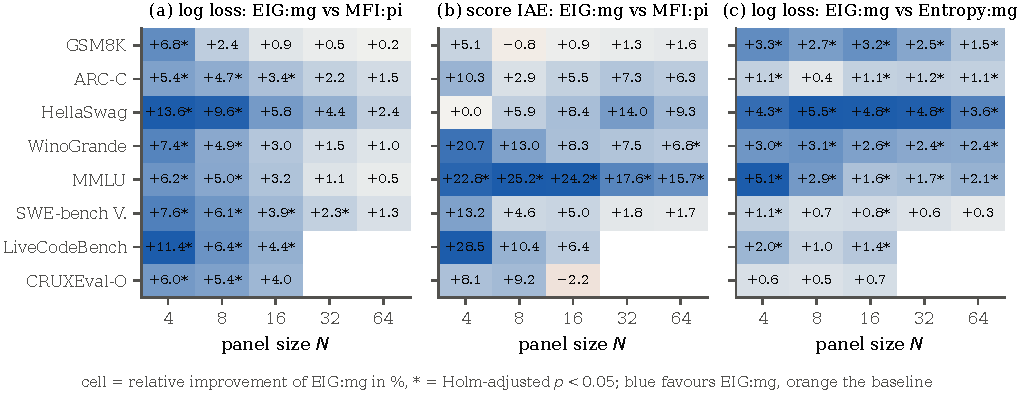
\includegraphics[width=\linewidth]{figures/heatmap_improvement.pdf}
\caption{Relative improvement (\%) of EIG:mg over the baseline for every benchmark and calibration-panel size; * marks Holm-adjusted $p<0.05$ (panels a and c: confirmatory family; panel b: secondary family). Blue favours EIG:mg.}
\label{fig:heatmap}
\end{figure}

\begin{figure}[tbp]
\centering
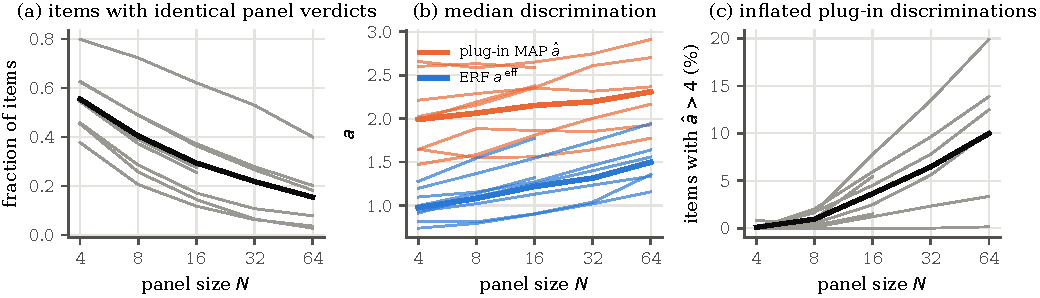
\includegraphics[width=\linewidth]{figures/calibration_diagnostics.pdf}
\caption{Calibration diagnostics on the study-1 benchmarks (thin lines: individual benchmarks; thick: mean). (a) Fraction of items that every calibrator answered identically, whose difficulty is identified only through the prior. (b) Median plug-in discrimination versus the effective discrimination of the expected response function. (c) Fraction of items whose plug-in discrimination exceeds 4 under the empirical-Bayes prior.}
\label{fig:diag}
\end{figure}

\begin{figure}[tbp]
\centering
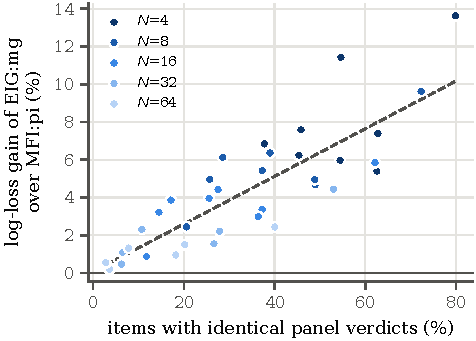
\includegraphics[width=0.55\linewidth]{figures/mechanism.pdf}
\caption{Exploratory: the log-loss gain of EIG:mg over plug-in Fisher CAT grows with the fraction of items that the calibration panel cannot locate (identical verdicts across calibrators). One point per benchmark and panel size; dashed: least-squares line.}
\label{fig:mechanism}
\end{figure}

\subsection{Learning curves}\label{sec:curves}
\ResultsCurves\ \ResultsEfficiency\ Table~\ref{tab:full} gives the held-out log loss, the
score error and the coverage of six of the policies on every bank, real or synthetic, and
every panel size, and Figure~\ref{fig:curves-brier} the holdout Brier score as items are
administered.

\begin{figure}[tbp]
\centering
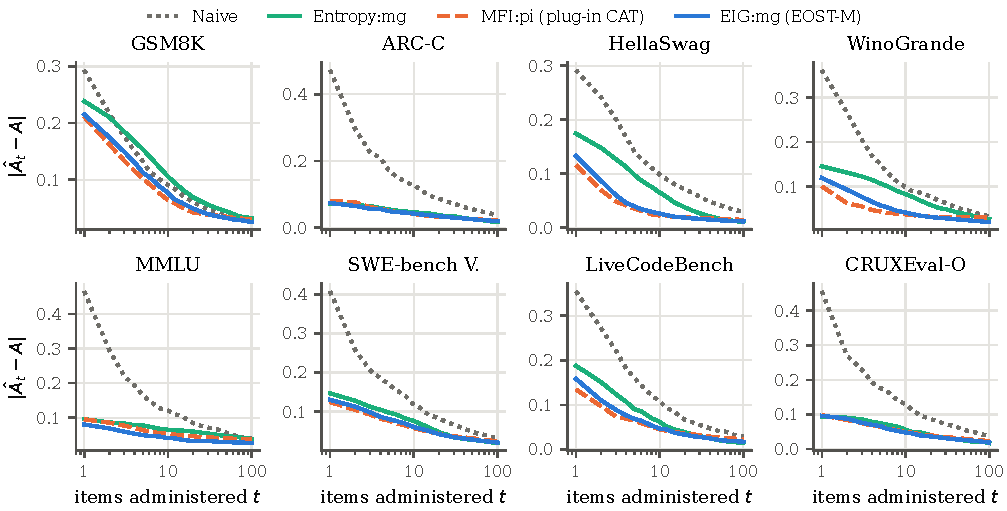
\includegraphics[width=\linewidth]{figures/curves_err_N8.pdf}
\caption{Absolute error of the full-bank score estimate as items are administered ($N=8$; mean over targets of per-target means over 5 replicates; logarithmic $t$ axis).}
\label{fig:curves-err}
\end{figure}

\begin{figure}[tbp]
\centering
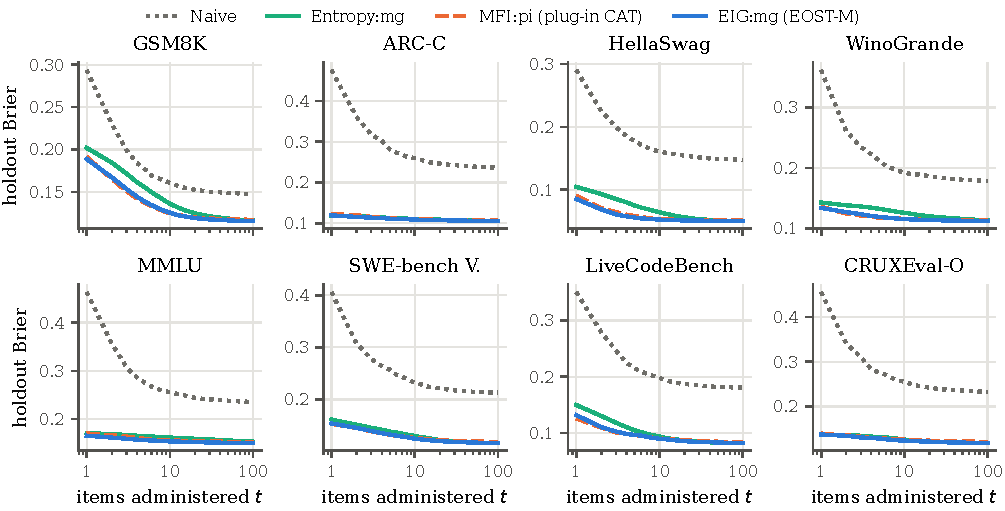
\includegraphics[width=\linewidth]{figures/curves_brier_N8.pdf}
\caption{Holdout Brier score as items are administered ($N=8$).}
\label{fig:curves-brier}
\end{figure}

\begin{table}[tbp]
\centering\footnotesize
\caption{All twelve policies at $N=8$, averaged over the eight confirmatory benchmarks (mean of per-benchmark means; in parentheses the mean rank across benchmarks, 1 = best). IAE: integrated absolute error of the full-bank score; $|\mathrm{cov}-0.9|$: miscalibration of the 90\% interval; $t_{0.03}$: sustained items-to-tolerance at $\varepsilon=0.03$ (101 = never).}
\label{tab:policies}
\setlength{\tabcolsep}{4pt}
\begin{tabular}{@{}lllll@{}}
\toprule
Policy & holdout log loss & score IAE & $|\mathrm{cov}-0.9|$ & $t_{0.03}$ \\
\midrule
Naive & -- & 0.0647 (11.5) & 0.0644 (1.1) & 86.3 (11.6) \\
Random:pi & 0.3720 (10.4) & 0.0424 (9.8) & 0.0972 (2.8) & 71.2 (10.0) \\
Random:mg & 0.3564 (6.1) & 0.0432 (10.0) & 0.0897 (2.2) & 71.5 (10.4) \\
Entropy:pi & 0.3724 (10.0) & 0.0398 (8.9) & 0.1598 (6.6) & 61.5 (8.8) \\
Entropy:mg & 0.3543 (5.6) & 0.0394 (8.4) & 0.1190 (4.9) & 64.0 (8.9) \\
MFI:pi (plug-in CAT) & 0.3666 (8.1) & 0.0341 (6.2) & 0.3088 (10.8) & 53.4 (5.1) \\
MFI:mg & 0.3470 (2.5) & 0.0301 (2.5) & 0.1677 (6.6) & 50.3 (4.0) \\
PWFI:mg & 0.3469 (2.1) & 0.0301 (2.1) & 0.1686 (7.1) & 49.9 (3.1) \\
EIG:pi & 0.3665 (7.8) & 0.0339 (6.0) & 0.3142 (11.4) & 53.6 (4.8) \\
EIG:mg \textbf{(EOST-M)} & 0.3473 (3.0) & 0.0309 (3.8) & 0.1746 (7.6) & 50.5 (3.8) \\
EVR:pi & 0.3665 (8.0) & 0.0340 (6.0) & 0.3051 (10.5) & 53.0 (4.2) \\
EVR:mg & 0.3471 (2.4) & 0.0303 (2.9) & 0.1664 (6.4) & 50.0 (3.4) \\
\bottomrule
\end{tabular}
\end{table}

\begin{table}[tbp]
\centering\footnotesize
\caption{Items needed to match the full-bank score error of 100 uniformly sampled items (Naive): first checkpoint $t$ at which the mean $|\hat A_t-A|$ over targets falls below the Naive error at $t=100$, at the primary panel size $N=8$ and at the largest panel available for the benchmark.}
\label{tab:efficiency}
\begin{tabular}{@{}lrrrrrr@{}}
\toprule
Benchmark & $N$ & Naive error @100 & Entropy:mg & MFI:pi & EIG:mg & EVR:mg \\
\midrule
GSM8K & 8 & 0.0296 & $>$100 & $>$100 & 70 & 80 \\
 & 64 & 0.0258 & $>$100 & 90 & 80 & 80 \\
\addlinespace[2pt]
ARC-C & 8 & 0.0364 & 25 & 15 & 20 & 12 \\
 & 64 & 0.0408 & 12 & 5 & 3 & 3 \\
\addlinespace[2pt]
HellaSwag & 8 & 0.0295 & 30 & 8 & 8 & 10 \\
 & 64 & 0.0306 & 10 & 3 & 3 & 4 \\
\addlinespace[2pt]
WinoGrande & 8 & 0.0326 & 80 & 20 & 20 & 15 \\
 & 64 & 0.0311 & 30 & 8 & 6 & 5 \\
\addlinespace[2pt]
MMLU & 8 & 0.0395 & 100 & 60 & 15 & 12 \\
 & 64 & 0.0396 & 25 & 6 & 5 & 6 \\
\addlinespace[2pt]
SWE-bench V. & 8 & 0.0334 & 40 & 50 & 40 & 40 \\
 & 64 & 0.0314 & 30 & 40 & 40 & 30 \\
\addlinespace[2pt]
LiveCodeBench & 8 & 0.0305 & 30 & 40 & 25 & 30 \\
 & 16 & 0.0298 & 25 & 20 & 15 & 20 \\
\addlinespace[2pt]
CRUXEval-O & 8 & 0.0359 & 25 & 30 & 25 & 20 \\
 & 16 & 0.0379 & 25 & 10 & 10 & 10 \\
\addlinespace[2pt]
\bottomrule
\end{tabular}
\end{table}


\ResultsLate

\begin{figure}[tbp]
\centering
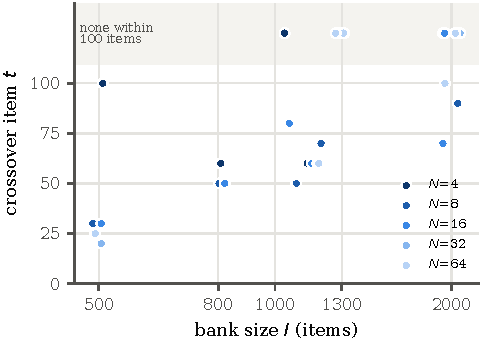
\includegraphics[width=0.55\linewidth]{figures/crossover.pdf}
\caption{Exploratory test of the regime change of Proposition~\ref{prop:evr}: the item after which entropy selection under the marginal model has a lower score error than EIG:mg at every later checkpoint, against the size of the bank. One point per benchmark and panel size (jittered horizontally); shaded band: no crossover within the 100-item budget.}
\label{fig:crossover}
\end{figure}

\begin{table}[p]
\centering\scriptsize
\caption{Full results: holdout log loss / score IAE / coverage of the 90\% interval (per-target means, then averaged over targets; leading zeros omitted).}
\label{tab:full}
\setlength{\tabcolsep}{2.5pt}
\begin{tabular}{@{}lrllllll@{}}
\toprule
Bank & $N$ & Naive & Entropy:mg & MFI:pi (plug-in CAT) & EIG:pi & EIG:mg & EVR:mg \\
\midrule
GSM8K & 4 & --/.051/.92 & .422/.069/.62 & .438/.054/.60 & .438/.055/.58 & .408/.052/.67 & .411/.055/.65 \\
GSM8K & 8 & --/.053/.89 & .388/.058/.67 & .387/.043/.67 & .387/.042/.68 & .378/.044/.70 & .379/.044/.69 \\
GSM8K & 16 & --/.054/.90 & .367/.053/.70 & .358/.038/.70 & .358/.038/.70 & .355/.037/.73 & .356/.039/.72 \\
GSM8K & 32 & --/.053/.91 & .348/.045/.73 & .341/.035/.70 & .341/.035/.70 & .340/.034/.73 & .341/.035/.73 \\
GSM8K & 64 & --/.053/.89 & .334/.041/.75 & .330/.035/.68 & .330/.035/.68 & .329/.035/.70 & .329/.035/.70 \\
\addlinespace[1pt]
ARC-C & 4 & --/.072/.90 & .383/.038/.87 & .400/.037/.56 & .401/.037/.58 & .378/.033/.78 & .377/.033/.77 \\
ARC-C & 8 & --/.073/.90 & .348/.029/.89 & .363/.029/.61 & .364/.030/.61 & .346/.029/.74 & .346/.027/.76 \\
ARC-C & 16 & --/.075/.89 & .325/.027/.87 & .332/.026/.58 & .332/.025/.59 & .321/.024/.70 & .321/.023/.71 \\
ARC-C & 32 & --/.076/.88 & .310/.026/.86 & .314/.024/.57 & .314/.024/.57 & .307/.022/.65 & .307/.023/.65 \\
ARC-C & 64 & --/.074/.88 & .303/.026/.82 & .304/.024/.55 & .303/.024/.55 & .299/.023/.60 & .299/.023/.60 \\
\addlinespace[1pt]
HellaSwag & 4 & --/.057/.90 & .213/.033/.76 & .236/.023/.60 & .237/.023/.58 & .204/.023/.78 & .205/.024/.80 \\
HellaSwag & 8 & --/.057/.90 & .188/.029/.80 & .197/.019/.59 & .195/.018/.58 & .178/.018/.76 & .178/.019/.77 \\
HellaSwag & 16 & --/.056/.91 & .167/.022/.84 & .168/.016/.60 & .168/.016/.61 & .158/.015/.73 & .159/.015/.74 \\
HellaSwag & 32 & --/.060/.88 & .156/.019/.83 & .156/.014/.64 & .157/.015/.63 & .149/.012/.72 & .149/.013/.72 \\
HellaSwag & 64 & --/.058/.91 & .148/.017/.82 & .146/.014/.64 & .145/.013/.64 & .143/.012/.68 & .143/.013/.68 \\
\addlinespace[1pt]
WinoGrande & 4 & --/.062/.91 & .408/.055/.76 & .427/.043/.47 & .427/.045/.45 & .396/.034/.79 & .397/.036/.79 \\
WinoGrande & 8 & --/.063/.89 & .379/.047/.81 & .387/.034/.50 & .386/.033/.50 & .367/.029/.75 & .366/.029/.76 \\
WinoGrande & 16 & --/.061/.91 & .356/.041/.82 & .357/.029/.55 & .358/.029/.54 & .347/.026/.68 & .347/.026/.68 \\
WinoGrande & 32 & --/.063/.90 & .342/.036/.79 & .339/.026/.54 & .339/.026/.54 & .334/.024/.62 & .334/.023/.63 \\
WinoGrande & 64 & --/.062/.90 & .332/.034/.76 & .327/.027/.49 & .327/.027/.49 & .324/.025/.54 & .324/.026/.53 \\
\addlinespace[1pt]
MMLU & 4 & --/.072/.89 & .530/.079/.70 & .536/.052/.59 & .542/.055/.58 & .503/.040/.80 & .503/.039/.81 \\
MMLU & 8 & --/.073/.91 & .482/.051/.87 & .492/.043/.51 & .493/.045/.48 & .468/.032/.77 & .468/.032/.77 \\
MMLU & 16 & --/.073/.90 & .445/.036/.91 & .452/.038/.47 & .451/.037/.47 & .438/.029/.69 & .437/.029/.70 \\
MMLU & 32 & --/.071/.91 & .420/.037/.86 & .418/.032/.47 & .418/.032/.48 & .413/.026/.64 & .413/.026/.64 \\
MMLU & 64 & --/.072/.89 & .412/.036/.84 & .405/.030/.47 & .406/.031/.48 & .403/.026/.60 & .403/.025/.60 \\
\addlinespace[1pt]
SWE-bench V. & 4 & --/.067/.90 & .416/.046/.79 & .445/.044/.62 & .445/.043/.66 & .411/.038/.79 & .410/.038/.80 \\
SWE-bench V. & 8 & --/.067/.89 & .384/.038/.83 & .406/.037/.66 & .408/.038/.65 & .381/.035/.76 & .380/.034/.79 \\
SWE-bench V. & 16 & --/.063/.92 & .356/.033/.84 & .367/.033/.68 & .368/.035/.67 & .353/.032/.75 & .353/.031/.75 \\
SWE-bench V. & 32 & --/.066/.90 & .339/.031/.83 & .345/.033/.65 & .345/.032/.66 & .337/.032/.69 & .337/.031/.70 \\
SWE-bench V. & 64 & --/.065/.91 & .329/.030/.83 & .332/.032/.67 & .332/.031/.68 & .328/.031/.70 & .326/.030/.72 \\
\addlinespace[1pt]
LiveCodeBench & 4 & --/.059/.94 & .324/.038/.81 & .359/.043/.53 & .356/.042/.53 & .318/.031/.80 & .321/.034/.78 \\
LiveCodeBench & 8 & --/.059/.94 & .281/.031/.85 & .297/.032/.60 & .298/.033/.59 & .278/.029/.76 & .278/.028/.76 \\
LiveCodeBench & 16 & --/.064/.91 & .262/.026/.87 & .270/.025/.68 & .271/.025/.67 & .258/.023/.77 & .260/.024/.76 \\
\addlinespace[1pt]
CRUXEval-O & 4 & --/.068/.92 & .419/.038/.89 & .443/.038/.69 & .438/.036/.70 & .416/.035/.83 & .415/.034/.84 \\
CRUXEval-O & 8 & --/.073/.89 & .384/.032/.89 & .404/.034/.64 & .401/.032/.66 & .382/.031/.77 & .380/.030/.79 \\
CRUXEval-O & 16 & --/.070/.89 & .361/.030/.87 & .374/.026/.69 & .375/.028/.66 & .359/.027/.75 & .359/.027/.75 \\
\addlinespace[1pt]
Synth. 2PL & 4 & --/.072/.89 & .566/.051/.89 & .577/.048/.77 & .576/.048/.77 & .561/.042/.86 & .563/.045/.86 \\
Synth. 2PL & 8 & --/.068/.92 & .538/.047/.90 & .539/.039/.84 & .539/.039/.84 & .533/.037/.89 & .534/.037/.89 \\
Synth. 2PL & 16 & --/.070/.90 & .516/.040/.92 & .514/.034/.85 & .514/.034/.85 & .511/.034/.89 & .511/.033/.89 \\
Synth. 2PL & 32 & --/.069/.91 & .502/.041/.90 & .496/.029/.88 & .496/.029/.88 & .495/.028/.89 & .495/.028/.89 \\
Synth. 2PL & 64 & --/.067/.91 & .494/.039/.92 & .487/.027/.88 & .487/.027/.88 & .487/.027/.89 & .487/.026/.89 \\
\addlinespace[1pt]
Synth. guessing & 4 & --/.070/.90 & .603/.054/.88 & .612/.050/.77 & .613/.051/.77 & .599/.044/.88 & .599/.045/.86 \\
Synth. guessing & 8 & --/.073/.88 & .579/.052/.89 & .580/.042/.81 & .580/.042/.81 & .573/.039/.88 & .574/.039/.88 \\
Synth. guessing & 16 & --/.069/.90 & .561/.046/.90 & .559/.035/.86 & .559/.035/.86 & .556/.033/.91 & .556/.033/.90 \\
Synth. guessing & 32 & --/.072/.89 & .549/.044/.92 & .545/.031/.88 & .545/.031/.88 & .543/.030/.90 & .543/.030/.91 \\
Synth. guessing & 64 & --/.068/.91 & .542/.044/.91 & .534/.028/.89 & .534/.028/.89 & .533/.026/.91 & .533/.026/.91 \\
\addlinespace[1pt]
Synth. 2-D & 4 & --/.069/.90 & .582/.053/.89 & .596/.054/.74 & .596/.053/.74 & .581/.049/.81 & .582/.051/.79 \\
Synth. 2-D & 8 & --/.069/.90 & .556/.048/.89 & .562/.048/.76 & .562/.048/.76 & .555/.045/.81 & .555/.045/.81 \\
Synth. 2-D & 16 & --/.072/.89 & .539/.047/.88 & .539/.043/.79 & .538/.042/.79 & .535/.040/.84 & .536/.041/.84 \\
Synth. 2-D & 32 & --/.068/.92 & .526/.042/.91 & .525/.038/.83 & .526/.038/.83 & .524/.038/.85 & .524/.038/.85 \\
Synth. 2-D & 64 & --/.069/.90 & .521/.046/.87 & .516/.037/.82 & .516/.037/.83 & .514/.036/.83 & .515/.036/.83 \\
\addlinespace[1pt]
\bottomrule
\end{tabular}
\end{table}


\subsection{Ranking systems}\label{sec:ranking}
\ResultsRanking

\IfFileExists{tables/ranking.tex}{\begin{table}[tbp]
\centering\scriptsize
\caption{Exploratory (not in the frozen plan): Kendall's $\tau$ between the full-bank score estimated after $t$ items and the true full-bank accuracy, across targets, at $N=8$ (one adaptive test per target; mean over 5 replicates).}
\label{tab:ranking}
\setlength{\tabcolsep}{2.0pt}
\begin{tabular}{@{}lcccccccccccc@{}}
\toprule
 & \multicolumn{4}{c}{$t=10$} & \multicolumn{4}{c}{$t=25$} & \multicolumn{4}{c}{$t=50$} \\
\cmidrule(lr){2-5}\cmidrule(lr){6-9}\cmidrule(lr){10-13}
Benchmark & Naive & MFI:pi & EIG:mg & EVR:mg & Naive & MFI:pi & EIG:mg & EVR:mg & Naive & MFI:pi & EIG:mg & EVR:mg \\
\midrule
GSM8K & 0.71 & 0.78 & 0.76 & 0.78 & 0.82 & 0.84 & 0.85 & 0.85 & 0.86 & 0.87 & 0.88 & 0.87 \\
ARC-C & 0.28 & 0.61 & 0.60 & 0.61 & 0.45 & 0.69 & 0.69 & 0.72 & 0.55 & 0.75 & 0.74 & 0.76 \\
HellaSwag & 0.25 & 0.64 & 0.65 & 0.61 & 0.37 & 0.75 & 0.75 & 0.76 & 0.47 & 0.79 & 0.80 & 0.80 \\
WinoGrande & 0.27 & 0.48 & 0.51 & 0.54 & 0.33 & 0.60 & 0.61 & 0.64 & 0.42 & 0.64 & 0.67 & 0.67 \\
MMLU & 0.42 & 0.67 & 0.70 & 0.72 & 0.56 & 0.74 & 0.77 & 0.79 & 0.62 & 0.77 & 0.80 & 0.81 \\
SWE-bench V. & 0.62 & 0.75 & 0.73 & 0.76 & 0.72 & 0.84 & 0.83 & 0.84 & 0.80 & 0.88 & 0.88 & 0.89 \\
LiveCodeBench & 0.57 & 0.72 & 0.76 & 0.70 & 0.73 & 0.79 & 0.82 & 0.80 & 0.76 & 0.86 & 0.87 & 0.86 \\
CRUXEval-O & 0.43 & 0.63 & 0.64 & 0.65 & 0.53 & 0.74 & 0.77 & 0.75 & 0.61 & 0.79 & 0.81 & 0.81 \\
\bottomrule
\end{tabular}
\end{table}
}{}

\subsection{Uncertainty}
\ResultsCoverage

\begin{figure}[tbp]
\centering
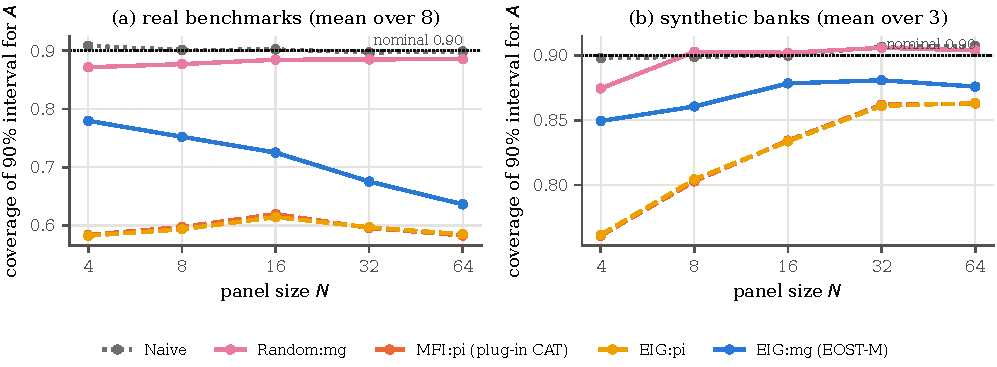
\includegraphics[width=\linewidth]{figures/coverage.pdf}
\caption{Coverage of the 90\% interval for the full-bank score, averaged over steps, targets and benchmarks, as a function of the panel size. Dotted line: nominal level.}
\label{fig:coverage}
\end{figure}

\subsection{Synthetic banks}\label{sec:synthetic}
\ResultsSynthetic

\begin{figure}[tbp]
\centering
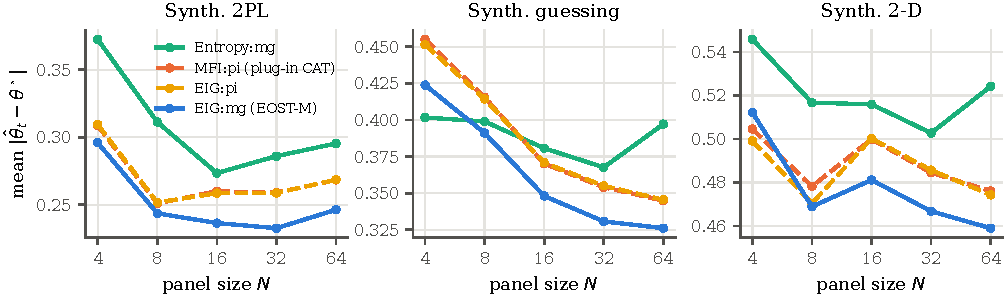
\includegraphics[width=\linewidth]{figures/synthetic_theta.pdf}
\caption{Error of the ability estimate with respect to the true generating ability on the three synthetic banks (well-specified 2PL; 60\% of items with a 0.25 guessing floor; two correlated ability dimensions), averaged over the 100-item test.}
\label{fig:synth}
\end{figure}

\subsection{Sensitivity analyses}\label{sec:sensitivity}
\ResultsSensitivity

\begin{table}[tbp]
\centering\footnotesize
\caption{Sensitivity analyses (30 targets, 3 replicates; main analysis for reference). Median relative improvement of EIG:mg across confirmatory benchmarks, in \%, [benchmarks improved / tested], and mean coverage of EOST-M's 90\% score interval. $^{\dagger}$Specified in the frozen plan, but its joint MAP is degenerate (the common discrimination diverges; Section~\ref{sec:sensitivity}), so its contrasts are not interpreted. $^{\ddagger}$Post hoc: common discrimination with prior $\log a\sim\mathcal N(0,0.05^2)$.}
\label{tab:sens}
\setlength{\tabcolsep}{3.5pt}
\begin{tabular}{@{}lrlllll@{}}
\toprule
Variant & $N$ & H1 log loss & H2 log loss & H3 IAE & H4 cov.\ gap & cov. \\
\midrule
main (EB prior, 2PL) & 8 & $+1.9$ [8/8] & $+5.2$ [8/8] & $+54.4$ [8/8] & $+44.2$ [8/8] & 0.75 \\
main (EB prior, 2PL) & 64 & $+1.8$ [6/6] & $+1.1$ [6/6] & $+62.1$ [6/6] & $+10.3$ [6/6] & 0.64 \\
fixed item prior & 8 & $+2.3$ [8/8] & $+2.8$ [5/8] & $+46.4$ [8/8] & $+35.8$ [5/8] & 0.70 \\
fixed item prior & 64 & $+2.2$ [6/6] & $+0.7$ [4/6] & $+63.2$ [6/6] & $+9.1$ [5/6] & 0.63 \\
near-duplicates removed & 8 & $+2.0$ [5/5] & $+6.1$ [5/5] & $+49.1$ [5/5] & $+46.2$ [4/5] & 0.73 \\
near-duplicates removed & 64 & $+2.2$ [5/5] & $+1.0$ [5/5] & $+66.4$ [5/5] & $+6.9$ [3/5] & 0.64 \\
\midrule
one-parameter$^{\dagger}$ & 8 & $-0.5$ [4/8] & $+38.9$ [8/8] & $-95.6$ [1/8] & $-3.8$ [3/8] & 0.15 \\
one-parameter$^{\dagger}$ & 64 & $-0.4$ [3/6] & $+45.0$ [4/6] & $-140.1$ [1/6] & $+0.9$ [4/6] & 0.20 \\
\midrule
one-parameter, regularized$^{\ddagger}$ & 8 & $+0.4$ [7/8] & $+0.7$ [7/8] & $+51.8$ [8/8] & $+14.3$ [8/8] & 0.84 \\
one-parameter, regularized$^{\ddagger}$ & 64 & $-0.2$ [2/6] & $0.0$ [3/6] & $+44.8$ [6/6] & $-3.3$ [3/6] & 0.81 \\
\bottomrule
\end{tabular}
\end{table}


\subsection{Post hoc probes that motivated study 2}\label{sec:strong}
After all frozen runs, three post hoc analyses with decision rules recorded before running
probed the main result: strong baselines, a regularization path of the discrimination prior
and a decomposition of interval coverage. \ResultsStrong

Because the regularized Rasch-type test is a strong competitor found after the fact,
study~2 tests it, together with a Bayesian CAT that also integrates the calibrators'
abilities, under a new frozen plan.

\IfFileExists{tables/posthoc.tex}{\begin{table}[tbp]
\centering\footnotesize
\caption{Post hoc comparison with strong baselines (not in the frozen plan; same targets, replicates, holdouts and calibration panels as the confirmatory study; decision rules recorded before the runs). Median relative improvement of EOST-M (EIG:mg) over each baseline across the eight benchmarks, in \%, with [benchmarks with a Holm-significant difference favouring EOST-M / favouring the baseline], Holm over this post hoc family, so that the counts for MFI:pi differ from Table~\ref{tab:confirm}; last column: mean coverage of the baseline's 90\% score interval at $N=8$.}
\label{tab:posthoc}
\setlength{\tabcolsep}{2.3pt}
\begin{tabular}{@{}lcccccc@{}}
\toprule
 & \multicolumn{3}{c}{holdout log loss} & score IAE & $|\mathrm{cov}-0.9|$ & cov. \\
\cmidrule(lr){2-4}\cmidrule(lr){5-5}\cmidrule(lr){6-6}\cmidrule(lr){7-7}
Policy & $N=4$ & $N=8$ & $N=16$ & $N=8$ & $N=8$ & $N=8$ \\
\midrule
EOST-M (EIG:mg), reference & -- & -- & -- & -- & -- & 0.75 \\
\midrule
plug-in 2PL (MFI:pi) & $+7.1$ [8/0] & $+5.2$ [5/0] & $+3.6$ [2/0] & $+7.5$ [1/0] & $+44.2$ [5/0] & 0.60 \\
plug-in posterior-mean 2PL, MFI & $+20.4$ [8/0] & $+15.5$ [7/0] & $+10.0$ [7/0] & $+7.3$ [2/0] & $+52.5$ [6/0] & 0.54 \\
plug-in posterior-mean 2PL, EIG & $+21.2$ [8/0] & $+14.7$ [7/0] & $+9.8$ [7/0] & $+7.7$ [2/0] & $+53.7$ [6/0] & 0.53 \\
plug-in regularized 1PL, MFI & $+2.9$ [4/0] & $+2.1$ [4/0] & $+3.3$ [5/0] & $+2.9$ [2/0] & $-25.9$ [0/0] & 0.81 \\
marginal regularized 1PL, EIG & $+1.0$ [3/0] & $+1.8$ [5/0] & $+2.8$ [4/0] & $+6.7$ [2/0] & $-54.0$ [0/1] & 0.83 \\
expected Fisher information (EFI:mg) & $0.0$ [0/0] & $0.0$ [0/0] & $0.0$ [0/0] & $+0.9$ [0/0] & $-3.0$ [0/0] & 0.76 \\
\bottomrule
\end{tabular}
\end{table}
}{}

\IfFileExists{figures/shrinkage_path.pdf}{%
\begin{figure}[tbp]
\centering
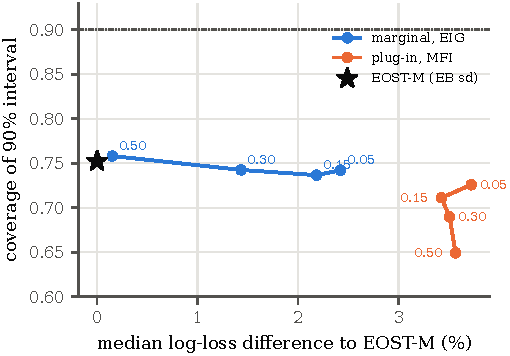
\includegraphics[width=0.55\linewidth]{figures/shrinkage_path.pdf}
\caption{Exploratory regularization path ($N=8$; planned before running): EOST-M's calibration with the prior standard deviation of $\log a$ fixed to the value next to each point instead of its empirical-Bayes estimate, for the marginal model with EIG and the plug-in model with MFI. Horizontal axis: median over benchmarks of the relative held-out log-loss difference to EOST-M; vertical axis: mean coverage of the 90\% score interval (dotted: nominal).}
\label{fig:shrink}
\end{figure}}{}

\IfFileExists{tables/coverage_decomp.tex}{\begin{table}[tbp]
\centering\footnotesize
\caption{Where the coverage of the 90\% score interval comes from (exploratory analysis of the post hoc runs, planned before computing; $N=8$). Coverage and score IAE (in percentage points) of EOST-M (EIG:mg) and of the regularized Rasch-type plug-in test (MFI:1pr), median over targets of the ratio of their mean interval widths (Rasch-type over EOST-M; Holm-significant on 8 of 8 benchmarks), and ratio of mean interval width to score IAE for plug-in 2PL (MFI:pi), EOST-M, the Rasch-type test and the marginal regularized one-parameter model (EIG:1prmg, column 1PL:mg). A calibrated 90\% interval for unbiased Gaussian errors has ratio $2\cdot1.645/\sqrt{2/\pi}=4.12$.}
\label{tab:covdecomp}
\setlength{\tabcolsep}{3pt}
\begin{tabular}{@{}lccccccccc@{}}
\toprule
 & \multicolumn{2}{c}{coverage} & width & \multicolumn{2}{c}{score IAE} & \multicolumn{4}{c}{width / IAE} \\
\cmidrule(lr){2-3}\cmidrule(lr){4-4}\cmidrule(lr){5-6}\cmidrule(l){7-10}
Benchmark & EOST-M & Rasch & ratio & EOST-M & Rasch & MFI:pi & EOST-M & Rasch & 1PL:mg \\
\midrule
GSM8K & 0.70 & 0.78 & 1.12 & 4.4 & 4.1 & 2.62 & 2.89 & 3.34 & 3.33 \\
ARC-C & 0.74 & 0.87 & 1.44 & 2.9 & 3.0 & 2.20 & 2.97 & 3.97 & 3.83 \\
HellaSwag & 0.76 & 0.79 & 1.14 & 1.8 & 1.7 & 2.00 & 2.88 & 3.21 & 3.46 \\
WinoGrande & 0.75 & 0.75 & 1.52 & 2.9 & 4.2 & 1.84 & 2.97 & 3.06 & 2.99 \\
MMLU & 0.77 & 0.81 & 1.76 & 3.2 & 5.3 & 1.90 & 3.22 & 3.40 & 3.68 \\
SWE-bench V. & 0.76 & 0.81 & 1.20 & 3.5 & 3.5 & 2.39 & 2.98 & 3.51 & 3.70 \\
LiveCodeBench & 0.76 & 0.81 & 1.08 & 2.9 & 2.7 & 2.26 & 3.11 & 3.53 & 3.83 \\
CRUXEval-O & 0.77 & 0.86 & 1.39 & 3.1 & 3.4 & 2.29 & 3.17 & 3.85 & 3.89 \\
\bottomrule
\end{tabular}
\end{table}
}{}

\section{Study 2: independent targets and strong competitors}
\label{sec:study2}

Study~2 evaluated \STwoTargetsTotal\ targets (between \STwoTargetsMin\ and
\STwoTargetsMax\ per benchmark, one per strict cluster) under the frozen plan of
Section~\ref{sec:design2}. Table~\ref{tab:study2} lists every decision,
Table~\ref{tab:study2banks} the main contrasts per benchmark, and
Table~\ref{tab:study2policies} the policy means. \StudyTwoSummary

\IfFileExists{tables/study2.tex}{\begin{table}[tbp]
\centering\footnotesize
\caption{Study 2: decisions under the frozen plan (primary panel size $N=8$; one target per strict family cluster). Holm sig.: benchmarks with a Holm-significant difference favouring EOST-M / favouring the competitor (Holm over the 88 superiority tests); positive: benchmarks on which EOST-M is better; median: median over benchmarks of the relative improvement of EOST-M (\%; for C3 the relative difference of the posterior-draw marginal (PDM) Bayesian CAT, for C5a the range of coverage). Supported: at least five benchmarks for EOST-M and none against (C3: equivalence on at least six; C5a: inside on at least six). $^\ast$C5a, C5b and C6 concern EOST-M's recalibrated interval.}
\label{tab:study2}
\setlength{\tabcolsep}{3pt}
\begin{tabular}{@{}lllcccl@{}}
\toprule
 & EOST-M versus & Endpoint & Holm sig. & positive & median & Supported \\
\midrule
R2 & plug-in 2PL (MFI:pi) & log loss & 5/0 & 8/8 & $+5.9$ & yes \\
R3 & Naive & score IAE & 6/0 & 8/8 & $+53.9$ & yes \\
R4 & plug-in 2PL (MFI:pi) & $|\mathrm{cov}-0.9|$ & 5/0 & 8/8 & $+41.6$ & yes \\
C1 & Rasch-type plug-in & log loss & 5/0 & 7/8 & $+2.4$ & yes \\
C2 & Rasch-type marginal & log loss & 4/0 & 8/8 & $+1.8$ & no \\
C4 & Random:mg & score IAE & 4/0 & 8/8 & $+21.1$ & no \\
C5b & raw EOST-M interval$^\ast$ & interval score & 0/2 & 4/8 & $+1.0$ & no \\
C6 & Naive (Wilson)$^\ast$ & interval score & 6/0 & 7/8 & $+35.0$ & yes \\
C7 & ATLAS-style 3PL CAT & score IAE & 4/0 & 8/8 & $+26.0$ & no \\
C8 & tinyBenchmarks & error @50 & 4/0 & 8/8 & $+29.6$ & no \\
C9 & MINCE & error @50 & 5/0 & 8/8 & $+44.8$ & yes \\
\midrule
C3 & PDM Bayesian CAT (equivalence) & log loss & \multicolumn{2}{c}{4/8 within $\pm$1\%} & $+0.32$ & no \\
C5a & (coverage in $[0.85,0.95]$)$^\ast$ & coverage & \multicolumn{2}{c}{5/8 banks inside} & 0.81--0.91 & no \\
\bottomrule
\end{tabular}
\end{table}
}{}
\IfFileExists{tables/study2_policies.tex}{\begin{table}[tbp]
\centering\footnotesize
\caption{Study 2: policy means at $N=8$ averaged over the eight benchmarks: integrated held-out log loss, integrated absolute score error, mean coverage and width of the 90\% score interval, and integrated interval score ($\alpha=0.1$; lower is better). Recalibrated intervals share the estimates of the raw policy.}
\label{tab:study2policies}
\setlength{\tabcolsep}{4pt}
\begin{tabular}{@{}lccccc@{}}
\toprule
Policy & log loss & score IAE & coverage & width & interval score \\
\midrule
EOST-M (EIG:mg) & 0.3582 & 0.0324 & 0.74 & 0.095 & 0.201 \\
EOST-M, recalibrated & (same) & 0.0324 & 0.86 & 0.134 & 0.206 \\
Rasch-type plug-in (MFI:1pr) & 0.3680 & 0.0344 & 0.81 & 0.121 & 0.220 \\
Rasch-type, recalibrated & (same) & 0.0344 & 0.91 & 0.271 & 0.321 \\
Rasch-type marginal (EIG:1prmg) & 0.3660 & 0.0366 & 0.82 & 0.128 & 0.214 \\
PDM Bayesian CAT, BMI (frozen burn-in) & 0.3599 & 0.0339 & 0.76 & 0.101 & 0.221 \\
PDM Bayesian CAT, EIG (frozen burn-in) & 0.3589 & 0.0326 & 0.77 & 0.101 & 0.210 \\
plug-in 2PL (MFI:pi) & 0.3825 & 0.0352 & 0.59 & 0.076 & 0.304 \\
ATLAS-style 3PL CAT & 0.3825 & 0.0448 & 0.48 & 0.085 & 0.417 \\
Random:mg & 0.3651 & 0.0422 & 0.88 & 0.162 & 0.211 \\
Naive (Wilson) & -- & 0.0640 & 0.90 & 0.235 & 0.290 \\
EOST-M, cross-fitted EB & 0.3583 & 0.0319 & 0.74 & 0.094 & 0.197 \\
EOST-M, Student-$t$ EB & 0.3601 & 0.0319 & 0.70 & 0.088 & 0.212 \\
mixed (every 4th random) & 0.3583 & 0.0326 & 0.77 & 0.102 & 0.189 \\
\bottomrule
\end{tabular}
\end{table}
}{}

\subsection{Replication with independent targets}
With one target per cluster, EOST-M's held-out log loss was lower than plug-in Fisher
CAT's on \STwoRTwoPos\ of 8 benchmarks (median \STwoRTwoMed\%), Holm-significantly on
\STwoRTwoFav\ and in favour of the baseline on \STwoRTwoBase: replication R2 is
\STwoRTwoVerdict. Its score error was \STwoRThreeMed\% below that of naive subsampling
(R3, \STwoRThreeVerdict; \STwoRThreeFav\ benchmarks significant), and its intervals were
less miscalibrated than plug-in Fisher CAT's by a median of \STwoRFourMed\% (R4,
\STwoRFourVerdict). \StudyTwoReplicationText

\IfFileExists{tables/study2_banks.tex}{\begin{table}[tbp]
\centering\footnotesize
\caption{Study 2 per benchmark ($N=8$): number of targets (independent clusters) and relative improvement (\%) of EOST-M over each competitor; * Holm-significant. $^\dagger$Recorded aggregate verdicts.}
\label{tab:study2banks}
\setlength{\tabcolsep}{4pt}
\begin{tabular}{@{}lrrrrrr@{}}
\toprule
 & & \multicolumn{3}{c}{held-out log loss} & \multicolumn{2}{c}{score IAE} \\
\cmidrule(lr){3-5}\cmidrule(l){6-7}
Benchmark & targets & MFI:pi & Rasch plug-in & Rasch marg. & Random:mg & ATLAS \\
\midrule
GSM8K & 40 & $+5.3$* & $+1.7$ & $+0.3$ & $+22.0$* & $+3.4$ \\
ARC-C & 40 & $+4.5$ & $+2.0$* & $+1.7$* & $+12.8$ & $+51.2$* \\
HellaSwag & 40 & $+12.2$* & $+6.4$* & $+1.3$ & $+43.1$* & $+38.0$* \\
WinoGrande & 40 & $+5.3$* & $+2.8$* & $+3.2$* & $+30.0$* & $+48.7$* \\
MMLU & 40 & $+7.2$* & $+4.7$* & $+5.0$* & $+5.0$ & $+24.1$ \\
SWE-bench V. & 40 & $+6.9$* & $+1.8$ & $+2.1$* & $+20.2$ & $+16.3$* \\
LiveCodeBench$^\dagger$ & 15 & $+6.4$ & $+3.4$* & $+1.9$ & $+46.7$* & $+27.9$ \\
CRUXEval-O$^\dagger$ & 12 & $+5.4$ & $-0.4$ & $+0.2$ & $+2.0$ & $+1.4$ \\
\bottomrule
\end{tabular}
\end{table}
}{}

\subsection{Integration, constraint, and Bayesian CATs}\label{sec:s2fb}
Against the regularized Rasch-type plug-in test, EOST-M's held-out log loss was lower on
\STwoCOnePos\ of 8 benchmarks (median \STwoCOneMed\%; \STwoCOneFav\ Holm-significant for
EOST-M, \STwoCOneBase\ for the competitor): C1 is \STwoCOneVerdict. Against the same
one-parameter model integrated over its item posterior, the median improvement was
\STwoCTwoMed\% (\STwoCTwoFav/\STwoCTwoBase; C2 \STwoCTwoVerdict). \StudyTwoRaschText
\par
The posterior-draw marginal (PDM) Bayesian CAT, which also integrates the calibrators'
abilities and the hyperprior through posterior draws, differed from EOST-M by a median of \STwoCThreeMed\% in held-out log loss and
was practically equivalent within $\pm1\%$ on \STwoCThreeEq\ of 8 benchmarks (C3
\STwoCThreeVerdict; Table~\ref{tab:equiv}). \StudyTwoFBText

\StudyTwoFBDetails

\IfFileExists{tables/fbfix.tex}{\begin{table}[tbp]
\centering\footnotesize
\caption{Study 2, Bayesian CATs against EOST-M at $N=8$ (post hoc correction of the burn-in and exploratory joint model; same targets, panels, holdouts and chains). Equivalence: 90\% bootstrap interval of the relative difference in held-out log loss within $\pm1\%$ (rule of C3: at least six benchmarks); median relative difference of log loss (positive: Bayesian CAT worse); benchmarks with a Holm-significant difference favouring EOST-M / the Bayesian CAT; the same for the score error (median relative improvement of EOST-M); mean coverage of the 90\% score interval (EOST-M: 0.74).}
\label{tab:fbfix}
\setlength{\tabcolsep}{3pt}
\begin{tabular}{@{}lcccccc@{}}
\toprule
 & \multicolumn{3}{c}{held-out log loss} & \multicolumn{2}{c}{score IAE} & \\
\cmidrule(lr){2-4}\cmidrule(lr){5-6}
Variant & equiv. & median \% & sig. & median \% & sig. & coverage \\
\midrule
PDM Bayesian, BMI (frozen, burn-in 10) & 4/8 & $+0.32$ & 0/0 & $+5.1$ & 0/0 & 0.76 \\
PDM Bayesian, EIG (frozen, burn-in 10) & 5/8 & $+0.18$ & 0/0 & $-0.8$ & 0/0 & 0.77 \\
PDM Bayesian, BMI (burn-in 60) & 3/8 & $+0.39$ & 0/0 & $+5.0$ & 0/0 & 0.76 \\
PDM Bayesian, EIG (burn-in 60) & 3/8 & $+0.50$ & 0/0 & $+4.2$ & 0/0 & 0.76 \\
joint fully Bayesian, BMI (exploratory) & 5/8 & $+0.33$ & 0/0 & $+2.8$ & 0/0 & 0.74 \\
joint fully Bayesian, EIG (exploratory) & 5/8 & $+0.05$ & 0/0 & $-1.5$ & 0/0 & 0.75 \\
\bottomrule
\end{tabular}
\end{table}
}{}
\IfFileExists{tables/equivalence.tex}{\begin{table}[tbp]
\centering\footnotesize
\caption{Study 2, hypothesis C3: relative difference (\%) of held-out log loss of the posterior-draw marginal (PDM) Bayesian CAT (Bayesian maximum information) with respect to EOST-M at $N=8$, its 90\% bootstrap interval over targets, and equivalence within $\pm1\%$.}
\label{tab:equiv}
\begin{tabular}{@{}lrcc@{}}
\toprule
Benchmark & difference & 90\% interval & equivalent \\
\midrule
GSM8K & +1.31 & [-0.71, +3.27] & no \\
ARC-C & +0.29 & [-0.12, +0.73] & yes \\
HellaSwag & +0.09 & [-0.32, +0.49] & yes \\
WinoGrande & -0.06 & [-0.28, +0.16] & yes \\
MMLU & +0.26 & [-0.20, +0.69] & yes \\
SWE-bench V. & +0.56 & [-0.02, +1.10] & no \\
LiveCodeBench & +0.99 & [-0.30, +2.27] & no \\
CRUXEval-O & +0.35 & [-0.81, +1.61] & no \\
\bottomrule
\end{tabular}
\end{table}
}{}
\IfFileExists{tables/fbfix_N4.tex}{\begin{table}[tbp]
\centering\footnotesize
\caption{Study 2, Bayesian CATs against EOST-M at $N=4$ (post hoc correction of the burn-in and exploratory joint model; same targets, panels, holdouts and chains). Equivalence: 90\% bootstrap interval of the relative difference in held-out log loss within $\pm1\%$ (rule of C3: at least six benchmarks); median relative difference of log loss (positive: Bayesian CAT worse); benchmarks with a Holm-significant difference favouring EOST-M / the Bayesian CAT; the same for the score error (median relative improvement of EOST-M); mean coverage of the 90\% score interval (EOST-M: 0.78).}
\label{tab:fbfixfour}
\setlength{\tabcolsep}{3pt}
\begin{tabular}{@{}lcccccc@{}}
\toprule
 & \multicolumn{3}{c}{held-out log loss} & \multicolumn{2}{c}{score IAE} & \\
\cmidrule(lr){2-4}\cmidrule(lr){5-6}
Variant & equiv. & median \% & sig. & median \% & sig. & coverage \\
\midrule
PDM Bayesian, BMI (frozen, burn-in 10) & 4/8 & $+0.33$ & 0/0 & $+2.6$ & 0/0 & 0.82 \\
PDM Bayesian, EIG (frozen, burn-in 10) & 4/8 & $+0.45$ & 0/0 & $+6.5$ & 0/0 & 0.79 \\
PDM Bayesian, BMI (burn-in 60) & 4/8 & $+0.21$ & 0/0 & $+1.6$ & 0/0 & 0.81 \\
PDM Bayesian, EIG (burn-in 60) & 2/8 & $+0.45$ & 1/0 & $+5.8$ & 1/0 & 0.79 \\
joint fully Bayesian, BMI (exploratory) & 4/8 & $-0.03$ & 0/0 & $+1.0$ & 0/0 & 0.79 \\
joint fully Bayesian, EIG (exploratory) & 4/8 & $+0.17$ & 0/0 & $-0.8$ & 0/0 & 0.79 \\
\bottomrule
\end{tabular}
\end{table}
}{}

\subsection{Adaptivity and benchmark-reduction methods}\label{sec:s2red}
All methods below use the same eight calibrators per target. ATLAS and tinyBenchmarks were
designed for panels of hundreds to thousands of systems, so these comparisons concern the
small-panel regime, not the methods in their native settings; MINCE targets few calibration
models. Under the same calibrated model, adaptive selection reduced the score error of random
items by a median of \STwoCFourMed\% (C4 \STwoCFourVerdict; \STwoCFourFav\ benchmarks
significant). Against the ATLAS-style 3PL CAT the median improvement in score error was
\STwoCSevenMed\% (C7 \STwoCSevenVerdict). After 50 items, EOST-M's score error was
\STwoCEightMed\% below tinyBenchmarks' gp-IRT (C8 \STwoCEightVerdict) and \STwoCNineMed\%
below MINCE's subset mean (C9 \STwoCNineVerdict); Table~\ref{tab:reduction} gives the
errors at 25, 50 and 100 items. \StudyTwoReductionText

\IfFileExists{tables/reduction.tex}{\begin{table}[tbp]
\centering\footnotesize
\caption{Study 2: absolute error of the full-bank score (percentage points) after 25, 50 and 100 items at $N=8$, averaged over targets and benchmarks. tinyBenchmarks and MINCE select their items without adapting to the target.}
\label{tab:reduction}
\begin{tabular}{@{}lccc@{}}
\toprule
Method & 25 items & 50 items & 100 items \\
\midrule
EOST-M (EIG:mg) & 3.39 & 2.81 & 2.13 \\
ATLAS-style 3PL CAT & 4.46 & 4.20 & 3.79 \\
Random:mg & 4.78 & 3.34 & 2.42 \\
tinyBenchmarks gp-IRT & 4.96 & 4.39 & 4.49 \\
tinyBenchmarks p-IRT & 4.69 & 3.92 & 3.31 \\
tinyBenchmarks anchors & 6.23 & 5.62 & 5.37 \\
MINCE subset mean & 6.71 & 4.69 & 3.19 \\
Naive (Wilson) & 7.05 & 4.88 & 3.26 \\
\bottomrule
\end{tabular}
\end{table}
}{}
\IfFileExists{tables/tiny_audit.tex}{\begin{table}[tbp]
\centering\footnotesize
\caption{Study 2, post hoc audit of tinyBenchmarks at $N=8$: percentage of cells (target $\times$ replicate) in which fewer anchor items than the budget were available: K-Means returns at most one anchor per distinct item embedding, and with eight calibrators the embeddings take only as many distinct values as there are distinct response patterns among the items, often fewer than 100; last column: median number of anchors actually used at a budget of 100.}
\label{tab:tinyaudit}
\begin{tabular}{@{}lcccc@{}}
\toprule
 & \multicolumn{3}{c}{cells with fewer anchors than budget (\%)} & anchors used \\
\cmidrule(lr){2-4}
Benchmark & 25 & 50 & 100 & at budget 100 \\
\midrule
GSM8K & 1 & 7 & 76 & 82 \\
ARC-C & 0 & 0 & 0 & 100 \\
HellaSwag & 0 & 0 & 29 & 100 \\
WinoGrande & 0 & 0 & 1 & 100 \\
MMLU & 0 & 0 & 0 & 100 \\
SWE-bench V. & 0 & 2 & 100 & 71 \\
LiveCodeBench & 0 & 0 & 98 & 67 \\
CRUXEval-O & 0 & 0 & 8 & 100 \\
\bottomrule
\end{tabular}
\end{table}
}{}

\subsection{Calibrated uncertainty}\label{sec:s2cov}
\StudyTwoCoverageText

\IfFileExists{figures/study2_coverage.pdf}{%
\begin{figure}[tbp]
\centering
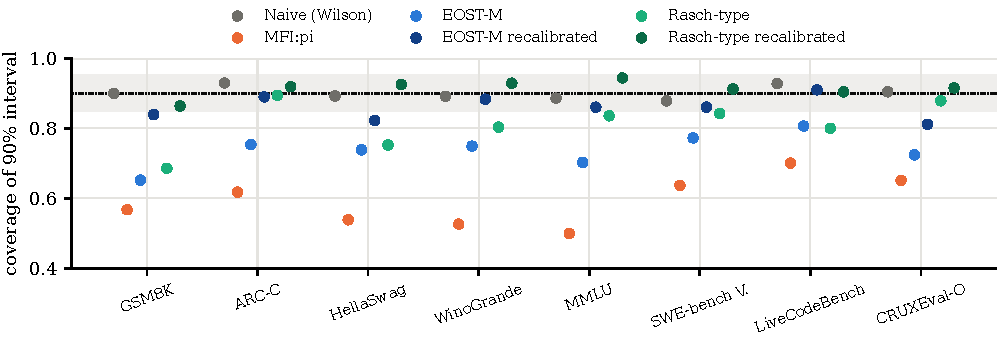
\includegraphics[width=\linewidth]{figures/study2_coverage.pdf}
\caption{Study 2: coverage of the 90\% score interval per benchmark at $N=8$ (mean over steps, replicates and targets). Shaded band: the $[0.85,0.95]$ criterion of hypothesis C5a; dotted: nominal.}
\label{fig:study2cov}
\end{figure}}{}

\subsection{Temporal validation and robustness}\label{sec:s2rob}
\StudyTwoRobustText

\subsection{Robustness of the empirical-Bayes hyperprior}\label{sec:eb}
The empirical-Bayes hyperprior is load-bearing: with a fixed weakly-informative prior,
the study-1 gain of EOST-M over plug-in Fisher CAT halves (Section~\ref{sec:sensitivity}).
Because it is estimated from the same panel, it could act as an opportunistic tuning
parameter. Stability and predictive checks (post hoc) and three alternatives run in study~2
under its frozen plan address this.

\paragraph{Stability.} Hyperparameters are re-estimated on bootstrap resamples of the items
(abilities held fixed), on two random halves of the items, and at $N=8$ on bootstrap
resamples of the calibrators (Table~\ref{tab:ebstab}). Resampling items moves them by at most
\EBItemsSdMaxEight\ (standard deviation, $N=8$): they pool hundreds of items and are well
determined given the panel. What varies is the panel: resampling calibrators moves the
spread of the log-discriminations by \EBCalSdSigmaA\ and that of the difficulties by
\EBCalSdSigmaB, comparable to the variation between panels (\EBBetweenSigmaA\ for
$\sigma_a$). The hyperprior therefore reflects which systems are in the panel, not noise
in the items.

\IfFileExists{tables/eb_stability.tex}{\begin{table}[tbp]
\centering\footnotesize
\caption{Stability of the empirical-Bayes hyperparameters (post hoc; three panels per benchmark and panel size). Medians over benchmarks of: the standard deviation across panels (between), the bootstrap standard deviation over items with abilities fixed (items), the absolute difference between fits on two random halves of the items (halves), and at $N=8$ the bootstrap standard deviation over calibrators (calibrators).}
\label{tab:ebstab}
\setlength{\tabcolsep}{3pt}
\begin{tabular}{@{}lccccccccc c@{}}
\toprule
 & \multicolumn{3}{c}{$N=4$} & \multicolumn{3}{c}{$N=8$} & \multicolumn{3}{c}{$N=16$} & $N=8$ \\
\cmidrule(lr){2-4}\cmidrule(lr){5-7}\cmidrule(lr){8-10}\cmidrule(l){11-11}
 & between & items & halves & between & items & halves & between & items & halves & calibrators \\
\midrule
$\mu_b$ & 0.17 & 0.09 & 0.16 & 0.07 & 0.07 & 0.11 & 0.08 & 0.07 & 0.07 & 0.10 \\
$\sigma_b$ & 0.11 & 0.09 & 0.10 & 0.16 & 0.07 & 0.10 & 0.18 & 0.07 & 0.05 & 0.15 \\
$\mu_a$ & 0.06 & 0.05 & 0.06 & 0.08 & 0.04 & 0.07 & 0.07 & 0.04 & 0.04 & 0.14 \\
$\sigma_a$ & 0.05 & 0.03 & 0.05 & 0.05 & 0.03 & 0.03 & 0.04 & 0.03 & 0.04 & 0.06 \\
\bottomrule
\end{tabular}
\end{table}
}{}

\paragraph{Prior predictive checks.} For each of the \PPCPanels\ panels (three per benchmark
and panel size), 200 response matrices were simulated from the fitted hyperprior given the
calibrators' abilities and compared with the observed matrix on three statistics; under a
correct model about 5\% of the two-sided predictive $p$-values would fall below 0.05. The
share of items that every calibrator or no calibrator answers correctly matters most for
Proposition~\ref{prop:cap}, because such items are located by the prior alone. It is
reproduced on average (median observed \PPCExtremeObs, simulated \PPCExtremeSim) but not
panel by panel: $p<0.05$ for \PPCExtremeLow\% of the panels (observed share higher than
simulated in \PPCExtremeAbove\%, lower in \PPCExtremeBelow\%), most of them on
HellaSwag and MMLU. The spread of the items' proportions correct is reproduced (observed
\PPCSdPObs, simulated \PPCSdPSim; $p<0.05$ for \PPCSdPLow\%). The mean item--rest
correlation is mostly lower than simulated (observed \PPCRestObs, simulated \PPCRestSim;
$p<0.05$ for \PPCRestLow\% of the panels, \PPCRestBelow\% below and \PPCRestAbove\% above),
again mainly on the multiple-choice banks of the Open LLM Leaderboard: real systems agree
with each other less, item by item, than a unidimensional 2PL with independent items
implies. The hyperprior therefore captures the distribution of item locations on which
EOST-M relies, while the response model is misspecified in its dependence structure, one
reason why model-based score intervals are too narrow (Section~\ref{sec:s2cov}).

\paragraph{Leave-item-block-out, other families, hierarchical Bayes.} Study~2 ran EOST-M
with a cross-fitted hyperprior (estimated, for every item, on the other half of the items,
so that no item informs its own prior) and with Student-$t$ hyperprior families ($\nu=4$) for
both item parameters; the Bayesian CATs integrate the hyperparameters instead of plugging
them in, which is the hierarchical Bayesian benchmark. Relative to EOST-M, the cross-fitted
variant left held-out log loss unchanged (median relative difference \SecXfVsEostMedAbs\%) and
the Student-$t$ variant made it slightly worse on every benchmark (median
\SecTpVsEostMedAbs\%), with no benchmark significant, and the Bayesian CATs were not
significantly different on any benchmark (Section~\ref{sec:s2fb}). The gain of
EOST-M therefore does not come from fitting the prior to the very items it is applied to,
nor from the Gaussian family or the plug-in hyperparameters.

\section{Robustness follow-ups after review}
\label{sec:s2follow}

\RobustIntro

\subsection{Clusters that never see the target's responses (RF1)}\label{sec:rf1}
\RobustClusterText

\IfFileExists{tables/robust_clusters.tex}{\begin{table}[tbp]
\centering\footnotesize
\caption{Robustness of study 2 to the clustering (follow-up RF1, planned before running). Frozen targets, holdouts and panel seeds; only the systems excluded from each target's panel change. For each exclusion rule: targets used, and for R2 (EOST-M vs plug-in Fisher CAT, log loss), C1 (vs the Rasch-type plug-in test, log loss) and C4 (vs Random:mg, score IAE): median relative improvement of EOST-M over benchmarks (\%), benchmarks with a positive difference, and benchmarks Holm-significant for / against EOST-M (frozen 88-test family with the rule's $p$-values substituted).}
\label{tab:robclust}
\setlength{\tabcolsep}{2.5pt}
\begin{tabular}{@{}lrrrrrrrrr@{}}
\toprule
 & & \multicolumn{3}{c}{R2} & \multicolumn{3}{c}{C1} & \multicolumn{2}{c}{C4} \\
\cmidrule(lr){3-5}\cmidrule(lr){6-8}\cmidrule(l){9-10}
Panel exclusion rule & targets & median & pos. & sig. & median & pos. & sig. & median & sig. \\
\midrule
frozen (joint residuals, $r\ge0.5$) & 267 & $+5.9$ & 8/8 & 5/0 & $+2.4$ & 7/8 & 5/0 & $+21.1$ & 4/0 \\
\midrule
metadata only (no responses) & 267 & $+5.9$ & 8/8 & 4/0 & $+2.4$ & 7/8 & 5/0 & $+20.5$ & 3/0 \\
leave-bank-out residuals & 267 & $+5.9$ & 8/8 & 5/0 & $+2.4$ & 7/8 & 5/0 & $+19.6$ & 3/0 \\
joint residuals, $r\ge0.4$ & 267 & $+5.9$ & 8/8 & 6/0 & $+2.4$ & 7/8 & 5/0 & $+19.5$ & 3/0 \\
joint residuals, $r\ge0.6$ & 267 & $+5.9$ & 8/8 & 4/0 & $+2.4$ & 7/8 & 5/0 & $+20.1$ & 3/0 \\
joint residuals, $r\ge0.7$ & 267 & $+5.9$ & 8/8 & 4/0 & $+2.4$ & 7/8 & 5/0 & $+18.3$ & 3/0 \\
\bottomrule
\end{tabular}
\end{table}
}{}
\IfFileExists{tables/robust_clusters_banks.tex}{\begin{table}[tbp]
\centering\scriptsize
\caption{Follow-up RF1 per benchmark: relative improvement (\%) of EOST-M in held-out log loss over plug-in Fisher CAT (R2) and over the Rasch-type plug-in test (C1) under each panel-exclusion rule; * Holm-significant (frozen 88-test family with the rule's $p$-values substituted). HS: HellaSwag; WG: WinoGrande; LCB: LiveCodeBench.}
\label{tab:robclustbanks}
\setlength{\tabcolsep}{2.5pt}
\begin{tabular}{@{}llrrrrrrrr@{}}
\toprule
Rule & & GSM8K & ARC & HS & WG & MMLU & SWE-V & LCB & CRUX-O \\
\midrule
metadata only & R2 & $+4.8$* & $+4.5$ & $+12.4$* & $+5.3$ & $+7.1$* & $+6.9$* & $+6.4$ & $+5.4$ \\
metadata only & C1 & $+1.9$ & $+1.9$* & $+6.7$* & $+2.9$* & $+4.9$* & $+1.8$ & $+3.4$* & $-0.4$ \\
leave-bank-out & R2 & $+4.0$ & $+4.6$* & $+12.2$* & $+5.2$* & $+6.7$* & $+6.9$* & $+6.4$ & $+5.4$ \\
leave-bank-out & C1 & $+1.8$ & $+1.9$* & $+6.4$* & $+2.9$* & $+5.1$* & $+1.8$ & $+3.4$* & $-0.4$ \\
joint, $r\ge0.4$ & R2 & $+5.1$* & $+4.5$* & $+12.5$* & $+5.1$* & $+7.6$* & $+6.9$* & $+6.4$ & $+5.4$ \\
joint, $r\ge0.4$ & C1 & $+1.8$ & $+1.9$* & $+6.7$* & $+2.8$* & $+3.9$* & $+1.8$ & $+3.4$* & $-0.4$ \\
joint, $r\ge0.6$ & R2 & $+4.8$ & $+4.6$* & $+12.2$* & $+5.2$ & $+7.1$* & $+6.9$* & $+6.4$ & $+5.4$ \\
joint, $r\ge0.6$ & C1 & $+1.9$ & $+1.9$* & $+6.4$* & $+3.0$* & $+5.0$* & $+1.8$ & $+3.4$* & $-0.4$ \\
joint, $r\ge0.7$ & R2 & $+4.8$* & $+4.5$ & $+12.2$* & $+5.3$ & $+7.0$* & $+6.9$* & $+6.4$ & $+5.4$ \\
joint, $r\ge0.7$ & C1 & $+1.7$ & $+1.9$* & $+6.6$* & $+2.9$* & $+5.1$* & $+1.8$ & $+3.4$* & $-0.4$ \\
\bottomrule
\end{tabular}
\end{table}
}{}
\IfFileExists{tables/robust_cluster_counts.tex}{\begin{table}[tbp]
\centering\footnotesize
\caption{Clusters under each panel-exclusion rule of follow-up RF1: number of clusters / size of the largest cluster. The five Open LLM Leaderboard banks share their systems and their joint clusters; leave-bank-out clusters differ per leaderboard bank (GSM8K shown).}
\label{tab:robclustcount}
\begin{tabular}{@{}lcccc@{}}
\toprule
Rule & Open LLM LB (GSM8K) & SWE-bench V. & LCB & CRUX-O \\
\midrule
frozen, $r\ge0.5$ & 176/39 & 92/64 & 15/4 & 12/9 \\
metadata only & 227/13 & 94/64 & 15/4 & 12/9 \\
leave-bank-out & 147/72 & 94/64 & 15/4 & 12/9 \\
joint, $r\ge0.4$ & 134/113 & 92/64 & 15/4 & 12/9 \\
joint, $r\ge0.6$ & 196/34 & 92/64 & 15/4 & 12/9 \\
joint, $r\ge0.7$ & 209/27 & 92/64 & 15/4 & 12/9 \\
\bottomrule
\end{tabular}
\end{table}
}{}

\subsection{MCMC quality of the Bayesian CATs (RF2--RF2d)}\label{sec:rf2}
\RobustMCMCDesign

\RobustMCMCFrozen

\IfFileExists{tables/robust_mcmc.tex}{\begin{table}[tbp]
\centering\scriptsize
\caption{MCMC convergence of the Bayesian CATs' sampler (follow-up RF2: the frozen sampler with long chains; 6 targets per benchmark, replicate 0, $N=8$; four chains, one from EOST-M's estimates and three from dispersed starts; burn-in 250, then 300 sweeps per chain with every third retained, 400 retained draws). Per benchmark and parameter: number of the six panels with rank-normalized split $\hat R<1.01$ / $\hat R<1.05$ / bulk ESS $\ge100$. Location: mean calibrator ability; scale: standard deviation of the calibrators' abilities (explanatory, not in the plan of RF2); $\mu_a,\sigma_a$: mean and standard deviation of the log discriminations, $\mu_b,\sigma_b$: of the difficulties. Last two columns: median and largest relative spread (\%) of the held-out log loss of the PDM Bayesian CAT (BMI) across the four chains. Summary rows over all panels: percentages; median (maximum) $\hat R$; median (minimum) bulk ESS; median Monte Carlo standard error as a percentage of the posterior standard deviation.}
\label{tab:rf2}
\setlength{\tabcolsep}{2pt}
\begin{tabular}{@{}lrrrrrrrr@{}}
\toprule
 & \multicolumn{6}{c}{panels with $\hat R<1.01$ / $\hat R<1.05$ / ESS $\ge100$} & \multicolumn{2}{c}{chain spread (\%)} \\
\cmidrule(lr){2-7}\cmidrule(l){8-9}
Benchmark & location & $\mu_b$ & $\sigma_b$ & $\mu_a$ & $\sigma_a$ & scale & median & max \\
\midrule
GSM8K & 6/6/6 & 0/3/2 & 0/0/0 & 0/0/0 & 0/0/0 & 0/0/0 & 8.9 & 43.3 \\
ARC-C & 1/6/6 & 6/6/6 & 0/0/0 & 0/0/0 & 0/0/0 & 0/0/0 & 1.0 & 1.7 \\
HellaSwag & 0/3/3 & 2/6/5 & 0/0/0 & 0/0/0 & 0/0/0 & 0/0/0 & 1.7 & 4.2 \\
WinoGrande & 0/5/4 & 4/5/5 & 0/0/0 & 0/1/0 & 0/0/0 & 0/0/0 & 0.9 & 1.3 \\
MMLU & 5/6/6 & 5/6/6 & 0/0/0 & 0/0/0 & 0/3/2 & 0/0/0 & 0.4 & 3.2 \\
SWE-bench V. & 6/6/6 & 6/6/6 & 0/0/0 & 0/0/0 & 0/0/0 & 0/0/0 & 1.1 & 2.6 \\
LiveCodeBench & 2/6/5 & 1/5/5 & 0/0/0 & 0/0/0 & 0/0/0 & 0/0/0 & 1.7 & 5.6 \\
CRUXEval-O & 3/6/6 & 6/6/6 & 0/0/0 & 0/0/0 & 0/1/0 & 0/0/0 & 0.8 & 5.5 \\
\addlinespace
all panels (\%) & 48/92/88 & 62/90/85 & 0/0/0 & 0/2/0 & 0/8/4 & 0/0/0 & 1.0 & 43.3 \\
$\hat R$, median (max) & 1.01 (1.10) & 1.01 (1.21) & 1.47 (2.46) & 1.50 (2.77) & 1.27 (3.04) & 1.40 (2.44) & & \\
bulk ESS, median (min) & 778 (35) & 612 (13) & 8 (5) & 8 (5) & 11 (5) & 9 (5) & & \\
MCSE / sd (\%) & 4 & 4 & 37 & 38 & 30 & 35 & & \\
\bottomrule
\end{tabular}
\end{table}

\begin{table}[tbp]
\centering\scriptsize
\caption{MCMC convergence of the exploratory samplers (follow-ups RF2b and RF2d; same panels, starting points and columns as Table~\ref{tab:rf2}; 400 retained draws). Upper block (RF2b): a Metropolis--Hastings move along the scale ridge added to every sweep of the frozen sampler. Lower block (RF2d): the model of Lemma~\ref{lem:exact} (item prior normalized over the grid) sampled with the hyperparameters, the scale and the location moved by Metropolis--Hastings steps with the item parameters summed out.}
\label{tab:rf2x}
\setlength{\tabcolsep}{2pt}
\begin{tabular}{@{}lrrrrrrrr@{}}
\toprule
 & \multicolumn{6}{c}{panels with $\hat R<1.01$ / $\hat R<1.05$ / ESS $\ge100$} & \multicolumn{2}{c}{chain spread (\%)} \\
\cmidrule(lr){2-7}\cmidrule(l){8-9}
Benchmark & location & $\mu_b$ & $\sigma_b$ & $\mu_a$ & $\sigma_a$ & scale & median & max \\
\midrule
\multicolumn{9}{@{}l}{\emph{RF2b: with the scale move, 4 chains, burn-in 200, 200 further sweeps per chain}} \\
GSM8K & 6/6/6 & 5/6/6 & 0/5/4 & 1/5/5 & 0/0/0 & 1/5/4 & 1.2 & 6.0 \\
ARC-C & 6/6/6 & 6/6/6 & 0/5/5 & 0/4/5 & 0/1/0 & 0/5/3 & 1.1 & 3.1 \\
HellaSwag & 1/2/2 & 2/6/5 & 0/1/1 & 0/0/1 & 0/0/0 & 0/1/1 & 2.0 & 5.6 \\
WinoGrande & 4/6/6 & 6/6/6 & 0/3/3 & 0/6/5 & 0/0/0 & 0/3/2 & 0.6 & 1.6 \\
MMLU & 6/6/6 & 5/6/6 & 0/5/5 & 0/5/6 & 0/4/0 & 1/5/5 & 0.5 & 1.3 \\
SWE-bench V. & 6/6/6 & 5/6/6 & 0/6/6 & 1/6/6 & 0/0/0 & 0/6/6 & 0.7 & 4.7 \\
LiveCodeBench & 5/6/6 & 5/6/6 & 0/4/4 & 0/6/6 & 0/0/0 & 0/5/5 & 1.9 & 3.0 \\
CRUXEval-O & 5/6/6 & 6/6/6 & 1/6/6 & 1/6/6 & 0/0/0 & 2/6/6 & 0.7 & 2.3 \\
\addlinespace
all panels (\%) & 81/92/92 & 83/100/98 & 2/73/71 & 6/79/83 & 0/10/0 & 8/75/67 & 1.0 & 6.0 \\
$\hat R$, median (max) & 1.00 (1.09) & 1.00 (1.04) & 1.04 (1.25) & 1.03 (1.32) & 1.31 (2.03) & 1.03 (1.26) & & \\
bulk ESS, median (min) & 552 (35) & 544 (97) & 153 (13) & 171 (10) & 11 (5) & 132 (12) & & \\
MCSE / sd (\%) & 4 & 4 & 8 & 8 & 32 & 9 & & \\
\midrule
\multicolumn{9}{@{}l}{\emph{RF2d: exact sampler of Lemma~\ref{lem:exact}'s model, 4 chains, burn-in 150, 200 further sweeps per chain}} \\
GSM8K & 6/6/6 & 3/6/6 & 0/2/3 & 0/3/3 & 1/6/5 & 0/4/3 & 1.3 & 26.0 \\
ARC-C & 1/5/5 & 0/4/5 & 0/6/5 & 0/2/1 & 0/1/1 & 0/6/5 & 0.3 & 0.8 \\
HellaSwag & 1/4/2 & 0/2/0 & 0/1/0 & 0/2/2 & 0/2/0 & 0/1/0 & 0.5 & 3.6 \\
WinoGrande & 0/4/3 & 0/0/0 & 0/0/0 & 0/0/0 & 0/5/5 & 0/2/1 & 0.7 & 1.5 \\
MMLU & 0/5/4 & 0/4/3 & 0/4/1 & 0/4/1 & 2/6/6 & 0/4/1 & 0.7 & 1.0 \\
SWE-bench V. & 6/6/6 & 5/6/6 & 0/2/0 & 0/1/0 & 1/6/5 & 0/1/0 & 1.2 & 3.1 \\
LiveCodeBench & 5/6/5 & 2/4/4 & 0/3/3 & 0/3/3 & 0/4/3 & 0/4/3 & 1.1 & 5.8 \\
CRUXEval-O & 2/6/6 & 1/6/4 & 0/5/4 & 0/5/3 & 0/5/5 & 0/6/4 & 0.6 & 5.7 \\
\addlinespace
all panels (\%) & 44/88/77 & 23/67/58 & 0/48/33 & 0/42/27 & 8/73/62 & 0/58/35 & 0.7 & 26.0 \\
$\hat R$, median (max) & 1.02 (1.09) & 1.03 (1.19) & 1.05 (1.25) & 1.06 (1.16) & 1.03 (1.20) & 1.04 (1.21) & & \\
bulk ESS, median (min) & 162 (42) & 129 (16) & 77 (13) & 72 (20) & 127 (15) & 85 (15) & & \\
MCSE / sd (\%) & 8 & 9 & 12 & 12 & 9 & 11 & & \\
\bottomrule
\end{tabular}
\end{table}
}{}
\IfFileExists{tables/robust_mcmc_arms.tex}{\begin{table}[tbp]
\centering\scriptsize
\caption{Bayesian CATs with frozen, corrected and long chains against EOST-M on the same 48 cells (follow-up RF2; 6 targets per benchmark, replicate 0, $N=8$). Median over cells of the relative difference in held-out log loss to EOST-M (\%; positive: worse than EOST-M); benchmarks whose median favours the arm / EOST-M; benchmarks with a median within $\pm1\%$; for the long chains, median signed and median absolute relative difference (\%) to the same arm with burn-in 60; mean coverage of the 90\% intervals. Exploratory follow-ups RF2b (sampler with the scale move) and RF2d (exact sampler of the model of Lemma~\ref{lem:exact}) are compared with the same arm with burn-in 60. PDM: posterior-draw marginal; joint: joint fully Bayesian (mixture over 40 of the retained draws); BMI: Bayesian maximum information; EIG: expected information gain.}
\label{tab:rf2arms}
\setlength{\tabcolsep}{4pt}
\begin{tabular}{@{}lrrrrrr@{}}
\toprule
 & \multicolumn{3}{c}{log loss vs EOST-M} & \multicolumn{2}{c}{vs burn-in 60 (\%)} & \\
\cmidrule(lr){2-4}\cmidrule(lr){5-6}
Arm & median (\%) & banks & $\pm1\%$ & signed & abs. & coverage \\
\midrule
EOST-M (empirical Bayes, no chain) & -- & -- & -- & -- & -- & 0.78 \\
\addlinespace
\multicolumn{7}{@{}l}{\emph{frozen arm of study 2: 1 chain, burn-in 10, 8 draws}} \\
\quad PDM, BMI & $+0.08$ & 4/4 & 6 & -- & -- & 0.82 \\
\quad PDM, EIG & $+0.06$ & 2/6 & 8 & -- & -- & 0.85 \\
\addlinespace
\multicolumn{7}{@{}l}{\emph{post hoc correction: 1 chain, burn-in 60, 8 draws}} \\
\quad PDM, BMI & $+0.37$ & 3/5 & 4 & -- & -- & 0.81 \\
\quad PDM, EIG & $+0.10$ & 3/5 & 6 & -- & -- & 0.84 \\
\quad joint, EIG & $+0.10$ & 4/4 & 5 & -- & -- & 0.81 \\
\quad joint, BMI & $+0.11$ & 5/3 & 7 & -- & -- & 0.80 \\
\addlinespace
\multicolumn{7}{@{}l}{\emph{RF2, long chains: 4 chains, burn-in 250, 400 draws (joint: 40)}} \\
\quad PDM, BMI & $+0.17$ & 3/5 & 8 & $+0.13$ & 1.02 & 0.86 \\
\quad PDM, EIG & $+0.04$ & 4/4 & 7 & $+0.11$ & 0.77 & 0.86 \\
\quad joint, EIG & $+0.20$ & 4/4 & 8 & $+0.05$ & 0.61 & 0.86 \\
\quad joint, BMI & $-0.45$ & 6/2 & 7 & $-0.25$ & 0.75 & 0.86 \\
\addlinespace
\multicolumn{7}{@{}l}{\emph{RF2b, scale move: 4 chains, burn-in 200, 400 draws (joint: 40)}} \\
\quad PDM, BMI & $+0.10$ & 4/4 & 5 & $-0.19$ & 0.77 & 0.85 \\
\quad PDM, EIG & $+0.01$ & 4/4 & 6 & $-0.05$ & 0.61 & 0.86 \\
\quad joint, EIG & $+0.07$ & 1/7 & 5 & $+0.15$ & 0.81 & 0.76 \\
\quad joint, BMI & $+0.29$ & 4/4 & 7 & $-0.02$ & 0.76 & 0.82 \\
\addlinespace
\multicolumn{7}{@{}l}{\emph{RF2d, exact sampler: 4 chains, burn-in 150, 400 draws (joint: 40)}} \\
\quad PDM, BMI & $-0.31$ & 5/3 & 7 & $-0.69$ & 1.62 & 0.78 \\
\quad PDM, EIG & $+0.15$ & 3/5 & 6 & $-0.29$ & 1.62 & 0.76 \\
\quad joint, EIG & $+0.20$ & 2/6 & 6 & $-0.16$ & 1.27 & 0.77 \\
\quad joint, BMI & $-0.13$ & 4/4 & 7 & $-0.14$ & 1.13 & 0.79 \\
\bottomrule
\end{tabular}
\end{table}
}{}

\IfFileExists{figures/rf2_traces.pdf}{%
\begin{figure}[tbp]
\centering
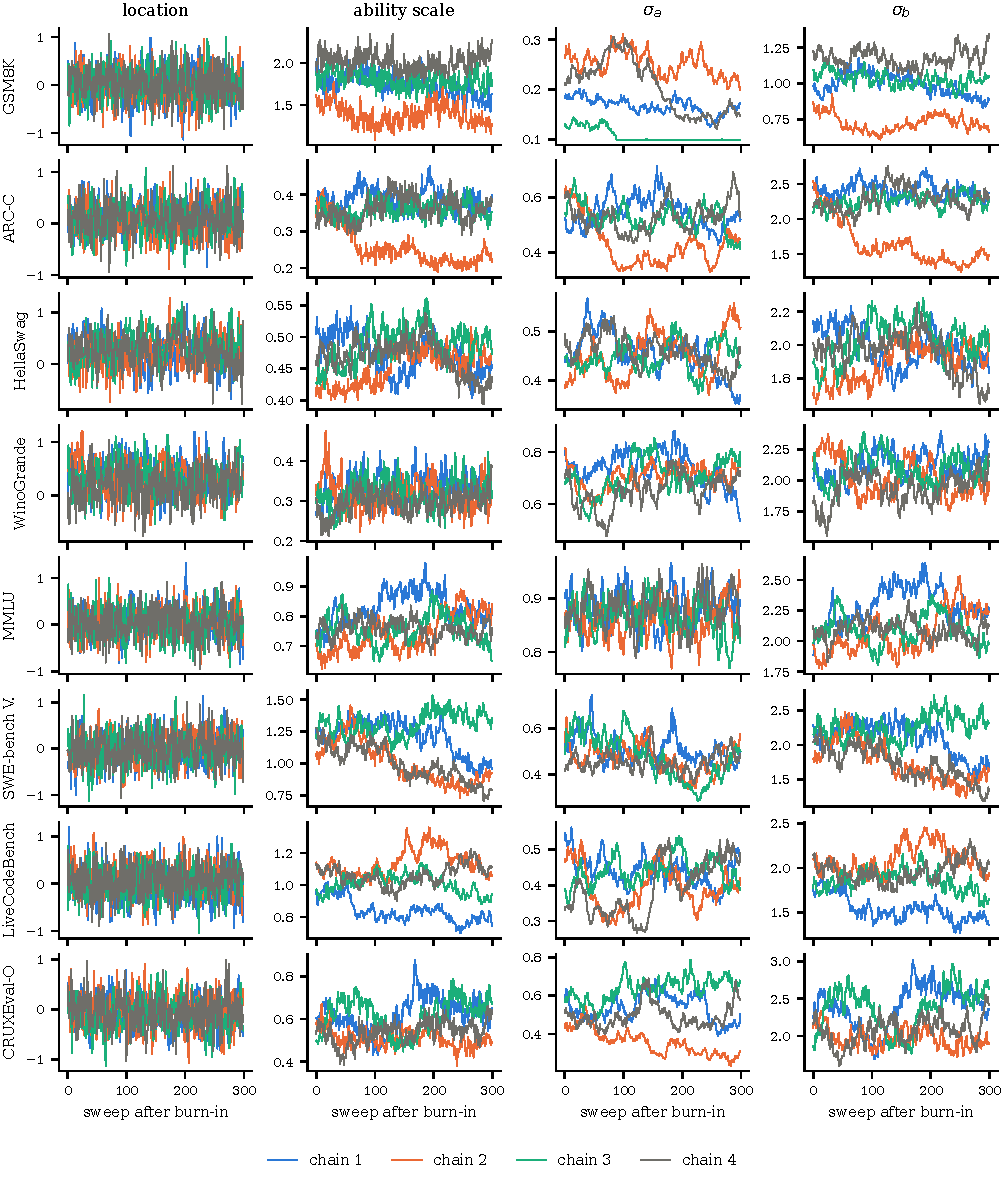
\includegraphics[width=\linewidth]{figures/rf2_traces.pdf}
\caption{Follow-up RF2: traces of the overall location (mean calibrator ability), the ability scale (standard deviation of the calibrators' abilities), $\sigma_a$ and $\sigma_b$ for the first selected panel of each benchmark; four chains (chain 1 starts at EOST-M's estimates), 300 sweeps after a burn-in of 250.}
\label{fig:rf2traces}
\end{figure}}{}

\IfFileExists{figures/rf2d_traces.pdf}{%
\begin{figure}[tbp]
\centering
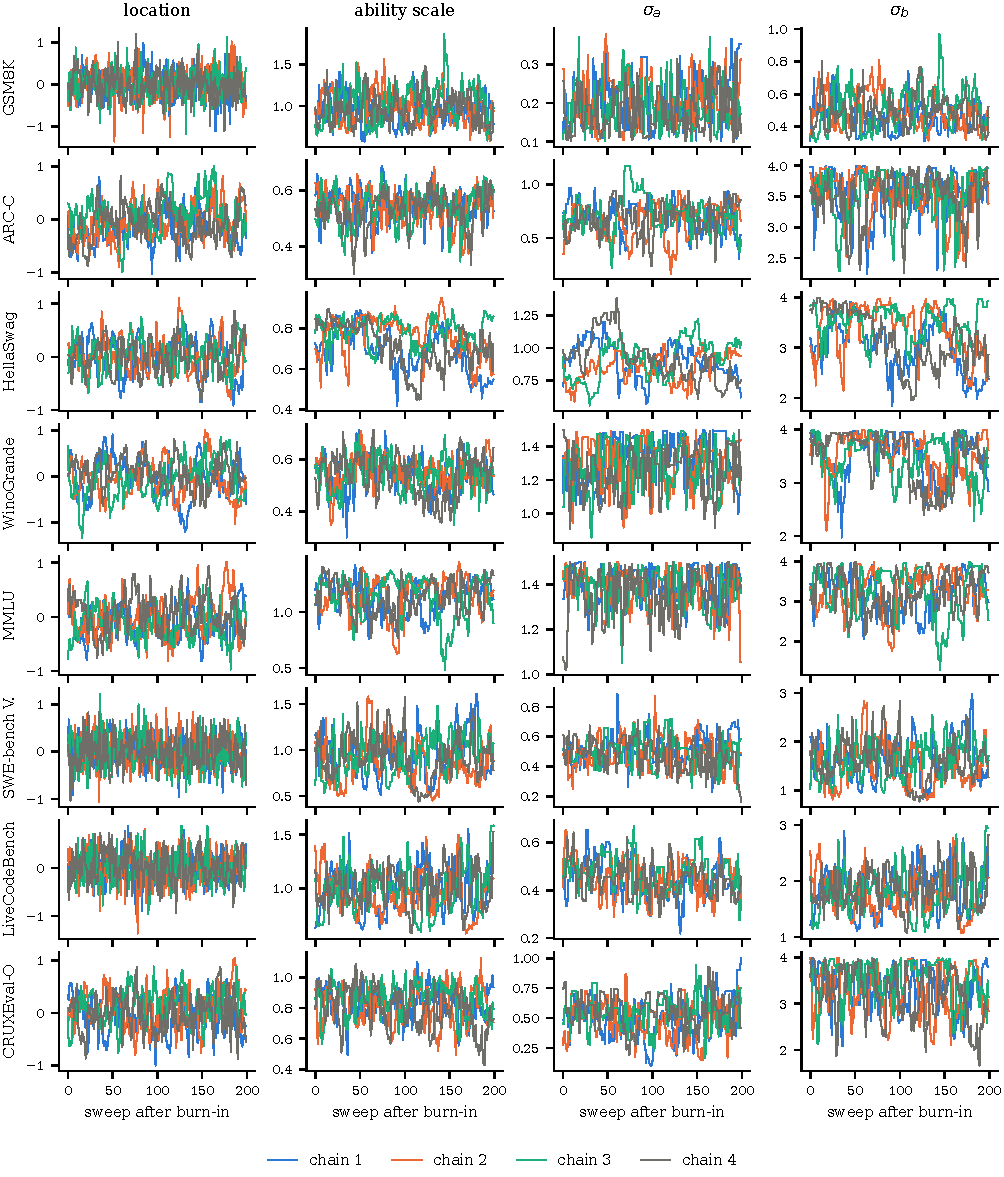
\includegraphics[width=\linewidth]{figures/rf2d_traces.pdf}
\caption{Exploratory follow-up RF2d (exact sampler of the model of Lemma~\ref{lem:exact}, with the hyperparameters, the scale and the location moved with the item parameters summed out): traces of the same quantities and panels as in Figure~\ref{fig:rf2traces}; four chains, 200 sweeps after a burn-in of 150.}
\label{fig:rf2dtraces}
\end{figure}}{}

\RobustMCMCScale

\RobustMCMCExact

\RobustMCMCConclusion

\FloatBarrier
\subsection{Effects across benchmarks (RF3, RF3b)}\label{sec:rf3}
\IfFileExists{tables/meta.tex}{\begin{table}[tbp]
\centering\footnotesize
\caption{Cross-benchmark effect of each study-2 superiority hypothesis (follow-up RF3, secondary; no frozen decision changes): random-effects pooled relative improvement of EOST-M (\%) over the eight benchmarks treated as independent, Hartung--Knapp--Sidik--Jonkman 95\% interval, 95\% prediction interval for a new benchmark, $I^2$ (\%), benchmarks with a positive effect and exact two-sided sign-test $p$; ``sources'': 95\% interval when the five Open LLM Leaderboard benchmarks, which share their 395 systems, count as one source (RF3b; four sources, 3 degrees of freedom); frozen decision. $^\ast$Recalibrated EOST-M interval.}
\label{tab:meta}
\setlength{\tabcolsep}{2.5pt}
\begin{tabular}{@{}lrccccccl@{}}
\toprule
EOST-M versus & pooled & 95\% CI & 95\% PI & $I^2$ & pos. & sign $p$ & sources & frozen \\
\midrule
R2 plug-in 2PL, log loss & $+6.0$ & [4.7, 7.2] & [4.3, 7.6] & 7 & 8/8 & 0.008 & [5.7, 7.6] & yes \\
R3 Naive, score IAE & $+50.5$ & [37.0, 64.0] & [24.2, 76.8] & 87 & 8/8 & 0.008 & [43.5, 57.5] & yes \\
R4 plug-in 2PL, $|\mathrm{cov}-0.9|$ & $+41.9$ & [35.3, 48.6] & [33.6, 50.3] & 6 & 8/8 & 0.008 & [34.0, 45.5] & yes \\
C1 Rasch-type plug-in, log loss & $+2.6$ & [1.2, 4.1] & [$-$0.2, 5.5] & 71 & 7/8 & 0.070 & [$-$0.4, 5.0] & yes \\
C2 Rasch-type marginal, log loss & $+2.0$ & [0.8, 3.2] & [$-$0.6, 4.7] & 75 & 8/8 & 0.008 & [1.4, 2.8] & no \\
C4 Random:mg, score IAE & $+23.4$ & [9.8, 37.1] & [$-$16.5, 63.3] & 88 & 8/8 & 0.008 & [$-$5.0, 52.6] & no \\
C5b raw interval$^\ast$, interval score & $-5.8$ & [$-$19.9, 8.3] & [$-$42.7, 31.0] & 82 & 4/8 & 1.000 & [$-$16.1, 10.0] & no \\
C6 Naive (Wilson)$^\ast$, interval score & $+29.8$ & [9.9, 49.7] & [$-$17.9, 77.5] & 91 & 7/8 & 0.070 & [18.7, 51.1] & yes \\
C7 ATLAS-style, score IAE & $+27.1$ & [11.2, 43.0] & [$-$20.0, 74.2] & 93 & 8/8 & 0.008 & [$-$1.1, 42.4] & no \\
C8 tinyBenchmarks, error @50 & $+34.5$ & [20.0, 49.0] & [$-$3.9, 72.9] & 80 & 8/8 & 0.008 & [$-$1.8, 76.7] & no \\
C9 MINCE, error @50 & $+41.9$ & [26.0, 57.8] & [1.2, 82.6] & 85 & 8/8 & 0.008 & [34.1, 49.3] & yes \\
\bottomrule
\end{tabular}
\end{table}
}{}

\RobustMetaText

\section{What adaptive evaluation costs}
\label{sec:cost}

Adaptive testing saves items only after somebody has answered the whole bank: the
calibration panel. Counting one administered item as the unit of cost, evaluating $M$ new
systems costs $MI$ with the full bank of $I$ items, and $NI+MT$ with a fresh panel of $N$
calibrators and adaptive tests of $T$ items, so adaptive testing pays off once
$M>NI/(I-T)$. With eight calibrators and $T=100$ this break-even lies between
\CostBreakFullMin\ and \CostBreakFullMax\ new systems on every benchmark
(Table~\ref{tab:cost}), and for
100 new systems the total cost is about \CostRatioHundred\% of full evaluation.

The fairer comparison is with uniform subsampling, which needs no panel at all. At
matched precision, EOST-M needed a median of \CostItemsNaive\ items to reach the score
error that 100 uniformly sampled items reach with the sample mean, so it saves about
\CostSaveNaive\ items per system but must first pay $NI$; the break-even is then a median of
\CostBreakNaiveMed\ new systems (from \CostBreakNaiveMin\ to \CostBreakNaiveMax\ across
benchmarks). Against Random:mg, which pays for the same panel, adaptivity alone saves
items from the first system on \CostRandomSaveBanks\ of 8 benchmarks: EOST-M matched 100
random items scored by the same model after a median of \CostItemsRandom\ items. Two situations change the arithmetic. When the
calibrators' full results already exist---public leaderboards, previous internal
evaluations---the panel is free and adaptive testing is cheaper from the first system.
When items are expensive to administer and a benchmark is used for many systems, as for
agentic benchmarks, the per-system saving dominates quickly. The computation itself is
negligible: calibrating a panel and running a 100-item test takes seconds on one CPU core
(Section~\ref{sec:design}).

\begin{table}[tbp]
\centering\footnotesize
\caption{Cost of adaptive evaluation with a fresh calibration panel of $N=8$ systems that must first answer all $I$ items (study 1). Break-even: number of new systems from which EOST-M with 100 items costs less than full evaluation; items for which EOST-M matches the score error of 100 uniformly sampled items scored by the sample mean (Naive) or by the same calibrated model (Random:mg), and the resulting break-even against Naive. When the calibrators' full results already exist (public leaderboards), the calibration cost vanishes and EOST-M is cheaper from the first system.}
\label{tab:cost}
\begin{tabular}{@{}lrrrrr@{}}
\toprule
 & & break-even vs & items to match & break-even vs & items to match \\
Benchmark & $I$ & full evaluation & Naive@100 & Naive & Random:mg@100 \\
\midrule
GSM8K & 1319 & 8.7 & 70 & 352 & 80 \\
ARC-C & 1172 & 8.7 & 20 & 117 & 90 \\
HellaSwag & 2000 & 8.4 & 8 & 174 & 25 \\
WinoGrande & 1267 & 8.7 & 20 & 127 & 60 \\
MMLU & 2000 & 8.4 & 15 & 188 & 100 \\
SWE-bench V. & 500 & 10.0 & 40 & 67 & 70 \\
LiveCodeBench & 1055 & 8.8 & 25 & 113 & 60 \\
CRUXEval-O & 800 & 9.1 & 25 & 85 & 60 \\
\bottomrule
\end{tabular}
\end{table}


\section{Discussion}
\label{sec:discussion}

\paragraph{Three messages.} \DiscussionSummary

\paragraph{Small-panel calibration uncertainty is the problem.} With four or eight
calibrators, a large fraction of items is answered identically by every calibrator, so
that their difficulty is located only by the prior (Figure~\ref{fig:diag}).
Plug-in testing treats these poorly located parameters as known: Fisher selection
credits such items with information they do not carry, the plug-in posterior becomes
overconfident, and the predicted outcomes of the unobserved items inherit the parameter
errors, which is the bias floor of Figure~\ref{fig:curves-err}. The expected response
function caps the information of an item whose difficulty is uncertain---at $2/(\pi s_i^2)$
for a Gaussian difficulty posterior with standard deviation $s_i$
(Proposition~\ref{prop:cap})---and predicts its outcome with the uncertainty it actually has; the empirical-Bayes
hyperprior keeps the predicted success probabilities of unlocated items sensible. Both
effects fade as the panel grows (Figure~\ref{fig:heatmap} and
Figure~\ref{fig:mechanism}). For the very large panels used by recent work
\citep{li2026atlas}, plug-in Fisher information is an adequate approximation; for new,
private or expensive benchmarks, self-generated item pools, or the four-to-eight-system
panels that a single laboratory can afford to run, it is not.

\paragraph{Integrating and constraining are two remedies.} \DiscussionRemedies

\paragraph{Why not always use a fully Bayesian adaptive test?} \DiscussionWhyNotFB

\paragraph{The criterion matters less than first hypothesized.} The pilot program and
study~1 agree on the direction of the original thesis---EIG learns more about
competence than predictive entropy---but also bound its size: once both criteria are
computed under the same calibration-marginal model, the gain on held-out prediction is
small, and EIG, maximum and posterior-weighted Fisher information and the score-targeted
criterion are practically interchangeable (Table~\ref{tab:policies}; a descriptive
comparison---the failure of H1 is not a test of equivalence).
Corollary~\ref{cor:blind} explains why: entropy and information disagree only through the
spread of discriminations among items with similar success probability, and the
expected response function shrinks discriminations towards what the panel can resolve.
The post hoc one-parameter variant confirms the mechanism: with a common discrimination
the EIG--entropy difference vanishes (Section~\ref{sec:sensitivity}). For the bank score
rather than competence, Proposition~\ref{prop:evr} shows that uncertainty sampling becomes
the right one-step criterion once competence is pinned down relative to the size of the
unobserved bank; the score-error curves show both regimes (Section~\ref{sec:curves}).
This is a negative result about the original hypothesis, and a useful one: what an
adaptive test for LLMs must get right is the treatment of calibration uncertainty, not
the choice among information criteria.

\paragraph{Honest uncertainty.} \DiscussionUncertainty

\paragraph{Adaptive testing or benchmark reduction?} \DiscussionReduction

\paragraph{A protocol for live evaluation.}\label{sec:live} Every result of this paper replays recorded verdicts. A live deployment differs in two
ways: the evaluated model has never been seen, and its answers are produced and graded at
the moment the test asks for them, with their sampling variability. We release the
protocol and code for such an experiment (\texttt{scripts/live\_eost.py}); it could not be
run in our execution environment, which has no access to model weights. The protocol has three
phases. (1) \emph{Freeze}: a calibration panel of $N$ leaderboard systems is
drawn with a fixed seed, excluding the target's family by a name pattern; the panel is
calibrated as in Section~\ref{sec:framework}; the leave-one-calibrator-out recalibration
factors are computed; the panel, seed, rule and a hash of the bank are written to
\texttt{frozen.json} before the first query. (2) \emph{Adaptive phase}: the model, served
through any OpenAI-compatible endpoint with temperature 0, answers the item chosen by EIG;
an independent deterministic oracle grades the answer (GSM8K: exact match of the final
number after the five-shot chain-of-thought prompt; CRUXEval-O: execution of
\texttt{assert f(input) == prediction} in an isolated subprocess); the estimate and both
intervals are recorded at every step, with checkpoints at 20, 40 and 60 items. (3)
\emph{Truth phase}: the remaining items are administered (answers already obtained are
reused) and the full-bank score is computed only after the adaptive phase is complete.
Every query, answer and verdict is appended to a log, so an interrupted run resumes.

The live engine performs exactly the computations of the replay
engine; a unit test feeds it recorded verdicts and checks that the selected items,
estimates and intervals coincide with the replay. A mock end-to-end run, in which a
recorded CRUXEval-O system answers through the live code path, reproduces the replay.
The OpenAI-compatible client is tested against a local server. Two differences from the
replay studies must be kept in mind when interpreting a live run: the target's prompt and
decoding may differ from those that produced the calibrators' verdicts (the Open LLM
Leaderboard used its own five-shot harness; CRUXEval-O verdicts aggregate samples at
temperature 0.2), and such a protocol shift is itself part of what a live run measures.

\paragraph{Limitations.} (i) All evidence replays recorded verdicts. Replay is exact for
the recorded data, but it does not include the sampling variability of stochastic
decoding, and the live protocol above could not be run in our
execution environment; the temporal validation on later SWE-bench submissions
approximates, but does not replace, a prospective deployment. (ii) Two confirmatory
benchmarks (LiveCodeBench, CRUXEval-O) carry recorded aggregate verdicts, binarized pass
rates over several samples; graded responses would need a different measurement model.
(iii) The measurement model is a unidimensional 2PL; prior predictive checks show that
real systems agree with each other less, item by item, than the model implies, mainly on
multiple-choice banks (Section~\ref{sec:eb}). (iv) Strict clusters are themselves a
heuristic: a residual correlation of 0.5 can miss distant relatives (distillation,
shared training data) and merge unrelated systems; one target per cluster removes the
dependence between targets, but calibrators drawn from other clusters may still share
ancestry with a target. The study-2 conclusions on R2 and C1 did not depend on how the
clusters were built---from metadata alone, from residuals on other benchmarks, or with
thresholds from 0.4 to 0.7 (Section~\ref{sec:s2follow}). (v) The leave-one-calibrator-out recalibration is a
cross-validated correction without a finite-sample guarantee; with eight calibrators it
rests on very few pseudo-targets. (vi) The frozen Bayesian CATs used a grid-based Gibbs
sampler with eight retained draws, whose scale hyperparameters did not converge even in long
chains; exploratory samplers with collapsed moves came close to convergence and left the
comparison with EOST-M unchanged, but a fully converged comparator---for instance by
Hamiltonian Monte Carlo on a continuous parametrization---remains to be run
(Section~\ref{sec:s2follow}). (vii) Both analysis plans were frozen by
hashing and committing them, and the second was also sent to the first author before
execution, but no public registry or external time stamp was reachable; a reader has to
trust the git history. (viii) Items were treated as equally costly and item exposure was
not controlled; an adaptive benchmark that serves the same few informative items to every
model would accelerate their contamination \citep{wainer2000cat}. (ix) Panels are
calibrated by joint maximum a posteriori estimation, which made the planned
one-parameter sensitivity analysis of study~1 degenerate (Section~\ref{sec:sensitivity});
marginal maximum likelihood over the calibrators' abilities avoids this class of
problems. (x) The self-testing side of the framework rests only on a historical pilot
(Section~\ref{sec:pilot}); a prospective study in which models generate items, an
independent oracle verifies them and a fresh panel calibrates them is the natural next
step. (xi) The cross-benchmark meta-analysis is secondary and treats the benchmarks as
independent, although five of them share the same systems; counted as one source, they leave
fewer pooled effects clear of zero (Section~\ref{sec:s2follow}).

\paragraph{Recommendations.} \RecommendationsText

\section{Conclusion}
\label{sec:conclusion}
\ConclusionText


% Acknowledgments and disclosure of funding (before the references)
\acks{This research did not receive any specific grant from funding agencies in the
public, commercial, or not-for-profit sectors. The authors declare no competing interests.
\emph{Data availability:} all response matrices are derived from public sources pinned to
git commits (Section~\ref{sec:repro}); matrices derived from MIT-licensed sources are
distributed with the code, and the others are rebuilt from the pinned sources by the
provided scripts and verified against published SHA-256 hashes. \emph{Code availability:}
the complete Docker-only pipeline, the frozen analysis plans, all artifacts and the
manuscript sources are released under the MIT licence at
\url{https://github.com/mesellemahmed/eost}.}


\vskip 0.2in
\bibliography{refs}

\end{document}
